\documentclass[11pt, twoside, onecolumn, a4paper, spanish]{book}

\usepackage{estilo_pfc}
\usepackage{graphics}
\usepackage{latexsym}
\usepackage{setspace}
\usepackage{rotate}
\usepackage{epsfig}
\usepackage{color}
\usepackage{wrapfig}
%\usepackage[bookmarks=true,bookmarksopen=truembookmarksnumber=true]{hyperref}

% Carga y configura el paquete listings para C
\definecolor{sourcecode}{rgb}{.8705,.8588,.8392}

\usepackage{listings}
\usepackage{lstlang2}
\lstset{
	language={C},
	extendedchars=true,
	tabsize=3,
	backgroundcolor=\color{sourcecode},
	frame=single, 
	framerule=0pt,
	basicstyle=\scriptsize,
	morekeywords={gint,gchar,gdouble,gfloat,gboolean,gpointer,FALSE,TRUE},
	commentstyle=\it,
	numbers=left,
	numberstyle=\tiny\sc,
	stepnumber=5,
	numbersep=0.5cm,
	escapechar=\@,
}


\begin{document}

\begin{titlepage}

\vspace*{-1.75cm}

\begin{center}

\scalebox{0.25}{
\includegraphics{udc_logo.eps}}

\vspace*{1.5cm}
\Large{\textbf{FACULTAD DE INFORM�TICA} \\}
\vspace*{0.5cm}
\Large{\textbf{Departamento de Computaci�n} \\}

\vspace{2cm}
\Large{\textbf{PROYECTO FIN DE CARRERA} \\}
\Large{\textbf{DE} \\}
\Large{\textbf{INGENIER�A T�CNICA EN \\ INFORM�TICA DE GESTI�N} \\}

\vspace{2.2cm}
{\Huge\textbf{Servicio de talk verbal para entornos Linux} \\}

\vspace{2.5cm}

\end{center}

\begin{flushleft}
\hspace*{6cm}\Large{\textbf{Autor}: \autor} \\
\hspace*{6cm}\Large{\textbf{Tutor}: \tutor} \\
\vspace{0.5cm}
\hspace*{6cm}\large{A Coru�a, Julio de 2003} \\
\end{flushleft}

\end{titlepage}




\thispagestyle{empty}

\vspace*{3cm}


D. Antonio Y��ez Izquierdo \\
\vspace*{1cm}

CERTIFICA 

\vspace*{2cm}

\begin{quotation}

 Que la memoria titulada \textbf{``Servicio de {\it talk} verbal para entornos
 Linux''} fue realizada por Jos� Riguera L�pez con D.N.I. 33.351.739-Z bajo
 su direcci�n. Esta documentaci�n constituye la documentaci�n que, con mi
 autorizaci�n, presenta el mencionado alumno para optar al grado de 
 Ingeniero t�cnico en Inform�tico de Gesti�n.

\end{quotation}

\vspace*{4cm}

\begin{flushright}
A Coru�a, Julio de 2003

\vspace*{3cm}

Firmado: Antonio Y��ez Izquierdo.
\end{flushright}

\newpage\thispagestyle{empty}

\section*{Especificaci�n}
\vspace*{2cm}

\begin{tabular}{p{4cm}p{7cm}}
\emph{T�tulo del proyecto}: &
\textbf{Servicio de {\it talk} verbal para entornos \emph{Linux}}

\end{tabular}

\vspace*{1cm}

\begin{tabular}{p{4cm}p{7cm}}
\emph{Clase}: & Proyecto cl�sico de ingenier�a.
\end{tabular}

\vspace*{1cm}

\begin{tabular}{p{4cm}p{7cm}}
\emph{Nombre del alumno}: & Jos� Riguera L�pez.
\end{tabular}

\vspace*{1cm}

\begin{tabular}{p{4cm}p{7cm}}
\emph{Nombre director}: & Antonio Y��ez Izquierdo.
\end{tabular}

\vspace*{1cm}

\begin{tabular}{p{4cm}p{7cm}}
\emph{Nombre del tutor}: & Antonio Y�ez Izquierdo.
\end{tabular}

\vspace*{1cm}

\begin{tabular}{p{4cm}p{7cm}}
\emph{Miembros del tribunal}: & $\ $\\
$\ $\\
$\ $\\
$\ $\\
$\ $
\end{tabular}

\vspace*{1cm}

\begin{tabular}{p{4cm}p{7cm}}
\emph{Miembros suplentes}: &$\ $\\
$\ $\\
$\ $\\
\end{tabular}

\vspace*{1cm}

\begin{tabular}{p{4cm}p{7cm}}
\emph{Fecha de lectura}: & $\ $\\
\end{tabular}

\vspace*{1cm}

\begin{tabular}{p{4cm}p{7cm}}
\emph{Calificaci�n}:
\end{tabular}

\newpage\thispagestyle{empty}

\vspace*{16cm}

\begin{flushleft}
\begin{scriptsize}
\begin{verbatim}
Copyright (c) 2003, Jos� Riguera. 
Permission is granted to copy, distribute and/or modify this 
document under the terms of the GNU Free Documentation License, 
Version 1.2 or any later version published by the Free Software
Foundation; with the Invariant Sections being: DEDICATORIA, 
AGRADECIMIENTOS and BIBLIOGRAF�A, with the Front-Cover Texts 
being PORTADA UDC, and with no Back-Cover Texts.

A copy of the license is included in the section of 
CD-ROM, `/docs/licencias/'.
\end{verbatim}
\end{scriptsize}
\end{flushleft}

\newpage\thispagestyle{empty}


\thispagestyle{empty}

\vspace*{7cm}

\begin{tabbing}
\hspace*{1cm}\= A todos aquellos que se esfuerzan para que la informaci�n no conozca barreras; \\
\> a todos los que apuestan por el poder del conocimiento y de la palabra, \\
\> y a Vd, estimado lector, que ya con el s�lo inter�s de leer estas l�neas \\
\> provoca que el autor se sienta orgulloso de esta obra. \\
\end{tabbing}


\thispagestyle{empty}

\vspace*{2cm}

\section*{Agradecimientos}

\vspace{1cm}

\begin{quote}
A Antonio Y��ez Izquierdo por aceptar y creer en este proyecto. \\
\end{quote}

\begin{quote}
A H�ctor Rivas por recomendarme no comer tantas pizzas, \\
a Mar�a Angueira por el nombre del programa, \\
a Rub�n L�pez por sus consejos. \\
y a todos aquellos que me conocen, por aguantarme estos �ltimos meses. 
 \end{quote}




\thispagestyle{empty}

\textbf{Resumen} \\

El objetivo del presente proyecto es la creaci�n de una aplicaci�n de VoIP que permita a varios usuarios comunicarse entre s� usando ordenadores normales (PC's). El programa se ejecuta en plataformas Linux y, mediante una conexi�n bidireccional RTP/RTCP, permite mantener una conversaci�n entre dos o m�s personas a modo de tel�fono. \\

La aplicaci�n tiene una arquitectura abierta y modular, que permite extender sus funcionalidades con tres tipos de plugins: E/S de audio, effectos sobre audio y codecs de compresi�n de voz. El programa es multisesi�n, es decir, puede mantener varias conversaciones activas simult�neamente, con o sin redes multicast. Tambi�n est� totalmente preparado para soportar la IPv6, la pr�xima generaci�n de IP. \\

Ha sido desarrollado con Glib-2.0 lo que garantiza que el sistema es portable entre plataformas Unix e incluso -con peque�as modificaciones- a plataformas MS Windows. La GUI se ha desarrollado en GTK+2.0 y es totalmente intuitiva, permite mostrar una imagen del usuario con el que est� dialogando y dispone de una agenda en XML en la que gestionar los contactos: a�adir, borrar, ignorar llamadas, etc.

\vspace{1.5cm}

\textbf{Palabras clave} \\
\\
\texttt{VoIP, RTP/RTCP, IPv6, Glib/GTK+, multicast, multisesi�n, plugins, Linux}



\newpage\thispagestyle{empty}
$\ $
\newpage\thispagestyle{empty}


\pagenumbering{roman}
\pagestyle{empty}
\dominitoc
\setcounter{page}{1}
\tableofcontents
\nuevoParrafo
                              
\pagenumbering{arabic}
\pagestyle{myheadings}
\setcounter{page}{1}

\capitulo{Introducci�n}
\label{chp:introduccion}
\minitoc
\newpage


\section{Pr�logo}

Tradicionalmente los servicios de telefon�a y de datos han estado soportados por sistemas de redes distintos, basadas en tecnolog�as muy diferentes. Para el transporte de voz se usaban -y usan- principamente las redes telef�nicas cl�sicas que emplean \emph{se�ales anal�gicas} junto con t�cnicas de \emph{conmutaci�n de circuitos}. Por otra parte las redes de datos telem�ticos son redes digitales y emplean una filosof�a basada en la \emph{conmutaci�n de paquetes}, como ocurre, por ejemplo, con el protocolo de Internet (\emph{IP}). \\

El desarrollo y maduraci�n de las t�cnicas de transmisi�n de voz sobre redes de paquetes ha dado lugar a una fuerte tendencia hacia la integraci�n del tr�fico de voz en las redes de datos. En la actualidad es frecuente escuchar t�rminos como ``convergencia de redes'' � ``convergencia de voz y datos'' para denominar a esta tendencia. Las ventajas que ofrece la convergencia de redes han sido en un principio de �ndole econ�mica. Tecnolog�as como \emph{VoIP} hacen un uso mucho m�s eficiente del ancho de banda de la red, y permiten ahorrar en los costes de gesti�n y mantenimiento de redes, ya que solamente se utiliza una �nica red para ambos servicios. \\

Sin embargo, no s�lo las razones econ�micas son las que justifican el inter�s en hacer converger las redes de voz y datos. La principal raz�n son las aplicaciones. La integraci�n de redes facilita la creaci�n de nuevas aplicaciones que comprenden voz y datos, como la mensajer�a unificada, que permitir� englobar bajo un �nico interfaz de usuario, accesible desde cualquier parte de la red, a todos los servicios a trav�s de los cuales recibir mensajes (correo electr�nico, fax, tel�fonos, contestadores, etc.). O, por citar otros ejemplos, la integraci�n de los centros de llamadas en los servidores web corporativos, que permitir�n una atenci�n r�pida y especializada a los clientes; las aplicaciones de videoconferencia, la teleense�anza, etc. Por otro lado, la utilizaci�n del protocolo \emph{IP} facilita la creaci�n de aplicaciones, ya que permite conectar la mayor�a de los dispositivos; basta con desarrollar la aplicaci�n una �nica vez y luego usarla en muchos tipos de redes diferentes. Aplicaciones que, aunque no t�cnicamente imposibles, ser�an de muy dif�cil realizaci�n sobre redes separadas. \\

Actualmente, gracias al avance tecnol�gico, ya es posible implantar, f�cil y pr�cticamente sin costos, un sistema de \emph{VoIP} en una red corporativa. Adem�s, las empresas de telecomunicaciones (Cisco, Ericsson, etc) ofrecen pasarelas capaces de enlazar redes datos \emph{IP} con las redes de telefon�a tradicional basadas en centrales telef�nicas de conmutaci�n (\emph{PBX}), permitiendo una implantaci�n completa e integral. \\

\begin{figure}[hbt]
\centering
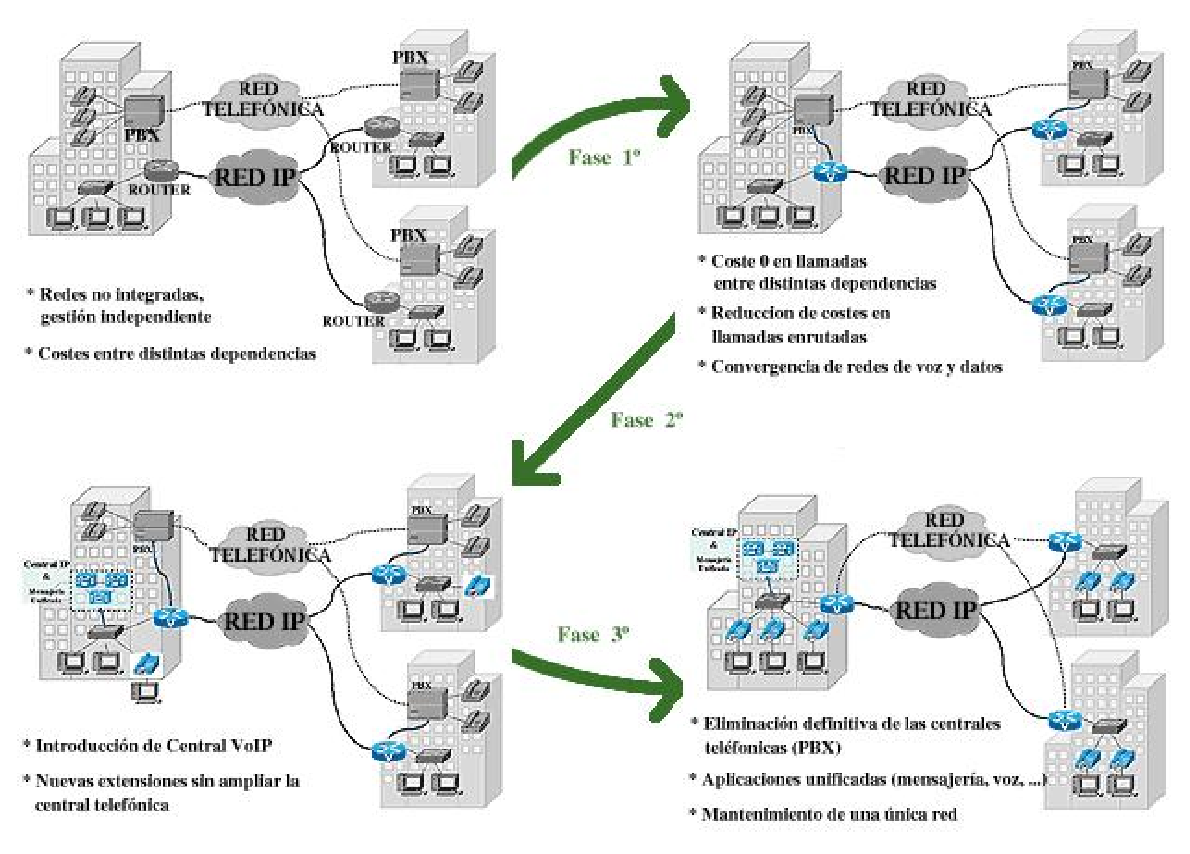
\includegraphics[width=\textwidth] {integracion_voip.eps}
\caption{Fases del proceso de integraci�n de las redes de voz y datos, con sus caracter�sticas y ventajas m�s destacables}
\label{fig:integracion_vopi}
\end{figure}


\section{Organizaci�n y contenido de esta memoria}

Esta memoria se ha estructurado del siguiente modo:\\

Tras una breve introducci�n en la que se detalla la importancia de la integraci�n de las redes de voz y datos, se procede a realizar un an�lisis de viabilidad (Cap�tulo \ref{chp:plan_proyecto}), en donde se describe el proyecto -objetivos, motivaciones, recursos, riesgos, etc.- y las principales decisiones preliminares adoptadas. En ese mismo cap�tulo se analizan los antecedentes y las caracter�sticas, dise�o, etc. de otras tecnolog�as u otras herramientas similares que van a rivalizar con este proyecto, es decir, se muestra el estado del arte. \\

A continuaci�n se introduce al lector en las tecnolog�as elegidas para el desarrollo del proyecto (cap�tulo \ref{chp:analisis_tecnologico}). Cabe resaltar que, debido a la multitud de tecnolog�as tratadas, no se profundizar� demasiado en cada una, pero, se tratar� lo m�nimo para que el lector comprenda los conceptos empleados en el proyecto, el trabajo de ampliar los conocimientos se deja al interesado. \\

En el siguiente cap�tulo se muestra las especificaciones y requerimientos. En base a esas especificaciones se realiza un dise�o (cap�tulo \ref{chp:diseno}), se detalla la organizaci�n y esctructura del sistema, en donde se muestran los subsistemas clave del proyecto y sus inter-relaciones. \\

Una vez inciado el desarrollo t�cnico, se exponen los detalles de la codificaci�n (cap�tulo \ref{chp:implementacion}). Se muestran todas las decisiones de implementaci�n tomadas. Se explican qu� algoritmos se aplicaron para resolver ciertos aspectos del dise�o, etc. En el siguiente cap�tulo se muestran algunas de las pruebas realizadas durante el desarrollo del proyecto junto con detalles del rendimiento del programa. \\

Tras la implementaci�n, se detallan los objetivos logrados, las ampliaciones realizadas al proyecto original, las posibles mejoras para versiones futuras, etc. Tambi�n se exponen las conclusiones alcanzadas una vez finalizado este trabajo. Todo esto en el �ltimo cap�tulo \ref{chp:conclusiones}. \\




\capitulo{Plan de proyecto}
\label{chp:plan_proyecto}
\minitoc
\newpage

Antes de la realizaci�n de un proyecto es necesario realizar una serie de an�lisis, m�s o menos profundos, dependiendo del tipo de sistema a desarrollar, para determinar su viabilidad y para intentar predecir los problemas que se encontrar�n. Por ejemplo, si los problemas de desarrollo superan a las espectativas, no compensar�a desarrollarlo. En este cap�tulo, se estudia el plan de proyecto para la propuesta m�nima realizada, es decir, sin tener en cuenta las ampliaciones.

\section{An�lisis de viabilidad}

Al emprender el desarrollo de un proyecto los recursos y el tiempo no son realistas para su materializaci�n, sin tener p�rdidas econ�micas ni frustraci�n profesional. La viabilidad y el an�lisis de riesgos est�n relacionados de muchas maneras, si el riesgo del proyecto es alto, la viabilidad de producir software de calidad se reduce. En el presente cap�tulo se tratar�n de definir estas �reas de inter�s:

\begin{description}
	\item [Descripcion] propuesta del proyecto.
	\item [Objeto]: motivos, necesidades y �mbito de la realizaci�n del proyecto.
	\item [Objetivos]: declaraci�n del objetivo final del proyecto.
	\item [Requerimientos y recursos necesarios] para el objetivo final.
	\item [Sistema de Control], seguimiento de los hitos obligados del proyecto.
	\item [Elementos de riesgo] que pueden hacer inviable el proyecto.
	\item [Beneficios] esperados tras la realizaci�n del proyecto.
	\item [Conclusiones]: posibilidades del proyecto.
\end{description}

\subsection{Descripci�n}

El proyecto consiste en el desarrollo de una aplicaci�n que use tecnolog�a de \emph{VoIP} para proveer un servicio de talk, parecido al que existe en entornos \emph{Unix}, pero con la particularidad de ser un servicio verbal, es decir, la aplicaci�n deber� permitir mantener una conversaci�n entre dos personas.
Para comenzar la conversaci�n, el usuario indicar� la direcci�n del otro interlocutor, y si �ste existe y acepta, se establecer� una conexi�n entre ambos usuarios que les permitir� mantener un di�logo ``full-duplex'' (bidireccional), de la misma forma que ocurre en la l�nea telef�nica tradicional. La direcci�n que especificar� cada usuario tendr� el formato de \emph{URL}, es decir, {\it \textbf{usuario}@\textbf{host}[:\textbf{puerto}]}; por ejemplo {\it \textbf{riguera}@\textbf{incertidumbre.dyndns.org}[:\textbf{10000}]}. \\

Ambos usuarios podr�n variar el volumen de los altavoces y la sensibilidad de sus micr�fonos. Una consideraci�n importante ser� el ancho de banda consumido por el proceso de comunicaci�n y el protocolo elegido para realizar la conexi�n. El ancho de banda y el protocolo elegido son dos caracter�sticas que depender�n del algoritmo de compresi�n de audio seleccionado. \\

El software ser� desarrollado lo m�s modular posible, es decir, que use ``plugins'' que implementen diferentes algoritmos de compresi�n para la transmisi�n del audio, es decir, un desarrollo con una arquitectura abierta. \\

Toda la documentaci�n y software del proyecto, una vez rematado �ste, quedar�n liberados bajo las licencias \emph{GFDL}\footnote{GNU Free Document License} y \emph{GPL}\footnote{GNU General Public License}, respectivamente.

\subsection{Objeto}

Este proyecto surgi� debido a la necesidad establecer una comunicaci�n f�cil y directa entre un grupo de desarrolladores de software. Un programador, en ocasiones, necesita hablar con el resto del grupo o con el jefe del proyecto para aclarar conceptos y, a veces, por problemas de espacio, est� en un local o despacho alejado. Aunque normalmente existe la posiblidad de usar el tel�fono, el mantenimiento y/o la instalaci�n de una central telef�nica -o del propio telef�no- puede resultar demasiado costoso. Tambi�n existen aplicaciones de mensajer�a instant�nea, pero es dif�cil escribir y discutir una idea por este sistema. La aplicaci�n anteriormente propuesta, podr�a ser capaz de solucionar gran parte de estas incomodidades. A continuaci�n se detallan sus ventajas e inconvenientes.

\paragraph{Ventajas:}
\begin{itemize}
	\item No es necesaria la disponibilidad de una red de voz ni de terminales telef�nicos.
	\item Mejor rendimiento de las infraestructuras. Permite un aprovechamiento de �ptimo de las redes de datos ya instaladas en la empresa.
	\item Poca p�rdida de tiempo, no es necesario conocer ni marcar ning�n n�mero tel�fonico; la conexi�n es inmediata.
	\item Actividad poco absorbente, el usuario puede hablar y hacer otra cosa al mismo tiempo, como por ejemplo escribir.
\end{itemize}

\paragraph{Inconvenientes,}las desventajas son muy pocas y f�cilmente salvables:

\begin{itemize}
	\item Es necesaria una red IP.
	\item El PC debe tener instalada y configurada una tarjeta de sonido, junto con altavoces y micr�fono.
\end{itemize}

\subsection{Objetivos}

En resumen, los \textbf{objetivos} m�nimos propuestos para la finalizaci�n de todo el proyecto son, ordenados por prioridad:

\begin{enumerate}
	\item Construir un programa capaz de comprimir y enviar el audio capturado por el micr�fono de un PC a otro y simult�neamente reproducir el audio recibido del PC remoto. El ordenador remoto efectuar� la misma operaci�n.
	\item El software deber� tener una interfaz gr�fica de usuario sencilla e intuitiva que permita realizar f�cilmente las conexiones.
	\item Los usuarios podr�n ajustar par�metros de audio tales como volumen y ganancia.
	\item Opcionalmente se considerar� la implementaci�n de un subsistema que use ``plugins'' y/u otras mejoras en el software.
	\item Realizaci�n de esta memoria.
\end{enumerate}

Las principales \textbf{restricciones} que tendr� el proyecto son:
\begin{itemize}
	\item El sistema se desarrollar� y documentar� empleando la metodolog�a de an�lisis y dise�o estructurado.
 	\item El programa se ejecutar� en m�quinas de capacidad media (PII o superior) y con un sistema operativo con soporte multitarea \emph{GNU/LINUX}, y en un entorno gr�fico \emph{Xwindows} (GNOME, KDE, etc)
	\item Tiempo limitado.
\end{itemize}

\subsection{Requerimientos y recursos}

\paragraph{Requerimientos,}para alcancar el objetivo final es necesario:

\begin{itemize}
	\item Un m�nimo de dos PC's con el sistema operativo \emph{Linux}. Se usan para recopilar informaci�n, analizar, dise�ar, programar y probar el software. Tambi�n es necesario que los PC's tengan sendas tarjetas de sonido configuradas y que est�n conectados por red \emph{IP}.
	\item Dos pares de altavoces o auriculares y un par de micr�fonos. Son necesarios para captar y reproducir el audio.
	\item Acceso a documentaci�n t�cnica sobre \emph{Linux}, muestreo de audio, compresi�n de audio, \emph{RFC's}, etc.
\end{itemize}

El tiempo m�ximo de elaboraci�n asciende al per�odo de un curso acad�mico, aproximadamente 9 meses, con dedicaci�n exlcusiva los �ltimos 6 meses y una �nica persona, que deber� planificar y realizar todas las fases del proyecto.

\paragraph{Recursos:}

Para la implementaci�n del programa ser� necesario evaluar el empleo de diferentes tecnolog�as de voz sobre \emph{IP} (\emph{VoIP}) tales como \emph{H323}, \emph{SIP}, etc. Los principales recursos provienen de Internet: {\it papers}, art�culos, foros, listas de correo electr�nico, manuales de programaci�n, ... Tambi�n resultan imprescindibles las bibliotecas de la \emph{UDC}\footnote{Universidade da Coru�a}, en especial, la biblioteca de la Facultad de Inform�tica. \\

En cuanto a los recursos software, cabe destacar los siguientes:

\begin{itemize}
	\item Distribuci�n \emph{Debian GNU/Linux} en su versi�n ``testing'' (Junio de 2003), conocida como ``\emph{Sarge}''.
	\item Herramintas gen�ricas de programaci�n, normalemente inclu�das en las distribuciones de Linux. Algunas de las m�s usuales son:
	\begin{description}
	   \item [Compiladores GNU]: {\it \textbf{gcc}}, {\it \textbf{gpc}}, {\it \textbf{g++}}, etc. En funci�n del lenguaje de programaci�n elegido.
       \item [Herramientas de depurado]: {\it \textbf{gdb}}, es el depurador cl�sico de entornos \emph{Unix}; �til para corregir todos los fallos de accesos no permitidos a memoria y excepciones de punto flotante. {\it \textbf{Electric-fence}} es una biblioteca que substituye la funci�n \emph{malloc} de la librer�a est�ndar, encargada de realizar las reservas de memoria, por una versi�n propia que incluye bandas de memoria no v�lidas entre cada par de bloques de memoria reservada, lo que permite detectar m�s f�cilmente desbordamientos de \emph{buffer}. {\it \textbf{Memprof}}, herramienta capaz de detectar fugas de memoria, es decir, bloques de memoria reservados din�micamente y ya no puede ser accedido, lo que hace imposible su liberaci�n.
       \item [Herramientas de control de tr�fico de red]: {\it \textbf{tcpdump}} y {\it \textbf{ethereal}}, permiten capturar parte del tr�fico que pasa por una interfaz de red aplicando filtros que eliminen los paquetes no deseados para realizar un an�lisis posterior. Permiten corregir fallos en la implementaci�n de los protocolos.
	\end{description}
	\item P�ginas del manual, documentan las funciones, librer�as y llamadas del sistema.
\end{itemize}

En general todos los recursos software empleados se caracterizar�n por ser ``open source'', es decir estar bajo la licencia {\it GPL}. Normalmente todos estos recursos ya vienen integrados en las distribuciones de \emph{Linux}; posteriormente se indicar� m�s detalladamente las herramientas empleadas.

\subsection{Sistema de Control}

El sistema de control de este proyecto est� basado en un calendario de actuaci�n, es decir, simplemente se controla el tiempo invertido en cada una de las fases o hitos. El tiempo m�ximo de realizaci�n es de 9 meses, con fecha limite de finalizaci�n el 4 de Julio de 2003. La fecha de la propuesta de este proyecto fue a finales de Mayo de 2002, si bien, no fue iniciado hasta Septiembre de 2002. Los hitos que comprende son:

\begin{enumerate}
	\item \textbf{Documentaci�n y viabilidad}: consiste en acaparar informaci�n de proyectos similiares, se buscan posibles tecnolog�as para el desarrollo del proyecto, etc. La fase acaba con un an�lisis de viabilidad y, si �ste es positivo, se elabora un \emph{Plan de proyecto}. En el caso de este proyecto, al ser de \emph{tipo B} -es decir, propuesto por el alumno- esta fase se elabor� antes de la propuesta, ya que el alumno no va a proponer un proyecto inviable, por esa raz�n el tiempo invertido en esta fase no entra dentro del tiempo m�ximo de realizaci�n, pero, se estima en 4-5 semanas.
	\item \textbf{An�lisis}: tras la \emph{Documentaci�n}, se procede al an�lisis de toda la informaci�n, se eval�a el uso de distintas tecnolog�as, se eligen las m�s adecuadas y se trazan las l�neas maestras del proyecto. Tiempo estimado:  4-5 semanas.
	\item \textbf{Dise�o, implementaci�n y pruebas}: durante el \emph{Dise�o} se establece la arquitectura del software, es decir, la definici�n de los subsistemas y subobjetivos. En conjunto, todos los subsitemas deben cumplir los requerimientos. El tiempo m�ximo de realizaci�n es de 1 mes. La \emph{Implementaci�n} del software, se basa en el \emph{Dise�o}: se implementa cada subsistema, se comprueba que cumple con los requisitos y se elaboran pruebas espec�ficas. Esta fase est� estrechamente relacionada con la anterior, de forma que el dise�o original puede sufrir modificaciones. 		   
	\item \textbf{Memoria}, es el documento final que analiza todas las fases del desarrollo del proyecto. Tiempo disponible para esta fase, 4 semanas.
\end{enumerate}

Este proyecto sigue un ciclo lineal, excepto en las fases de dise�o, implementaci�n y pruebas, el que el ciclo es evolutivo. Dicho de otro modo, las fases lineales son \emph{Documentaci�n} y \emph{An�lisis}, esto significa que ninguna de estas fases puede comenzar hasta que no haya terminado la anterior. Al final de cada una de estas dos fases se elabora un plan que define la actuaci�n en fases sucesivas. El ciclo evolutivo engloba el \emph{Dise�o, implementaci�n y pruebas}, ya que la etapa de dise�o puede sufrir modificaciones en funci�n de etapas sucesivas, y tambi�n, debido a las posibles ampliaciones del proyecto.

\subsection{Elementos de riesgo}

El principal riesgo del proyecto es el no cumplimiento de los hitos anteriores en el tiempo indicado y considerando que los plazos de entrega son fijos. Otros posibles riesgos proceden de la utilizaci�n de librer�as externas, que pueden presentar fallos de programaci�n (``bugs'') . Por estas circunstancias, los plazos de las distintas fases por las que atraviesa el proyecto, pueden acumular un retraso m�ximo total de 1 mes.

\subsection{Beneficios}

El objetivo de este proyecto no es conseguir beneficios econ�micos, simplemente se busca finalizar un ingenier�a t�cnica, por otro lado, este proyecto quedar� liberado bajo la \emph{GPL}, por lo que no tiene sentido plantearse beneficios econ�micos. \\

Sin embargo, las espectativas del este proyecto son altas. Existen cientos de previsiones que auguran crecimientos exponenciales al n�mero de minutos hablados a trav�s de VoIP, una explosi�n similar a la del uso del correo electr�nico a mediados de la d�cada de los noventa. La siguiente gr�fica (figura \ref{fig:espectativas_voip}) resume un estudio de Philips realizado en el a�o 2000, en la que se representa el porcentaje del total de tiempo de conversaci�n que se realizar� usando VoIP.

\begin{figure}[htb]
\centering
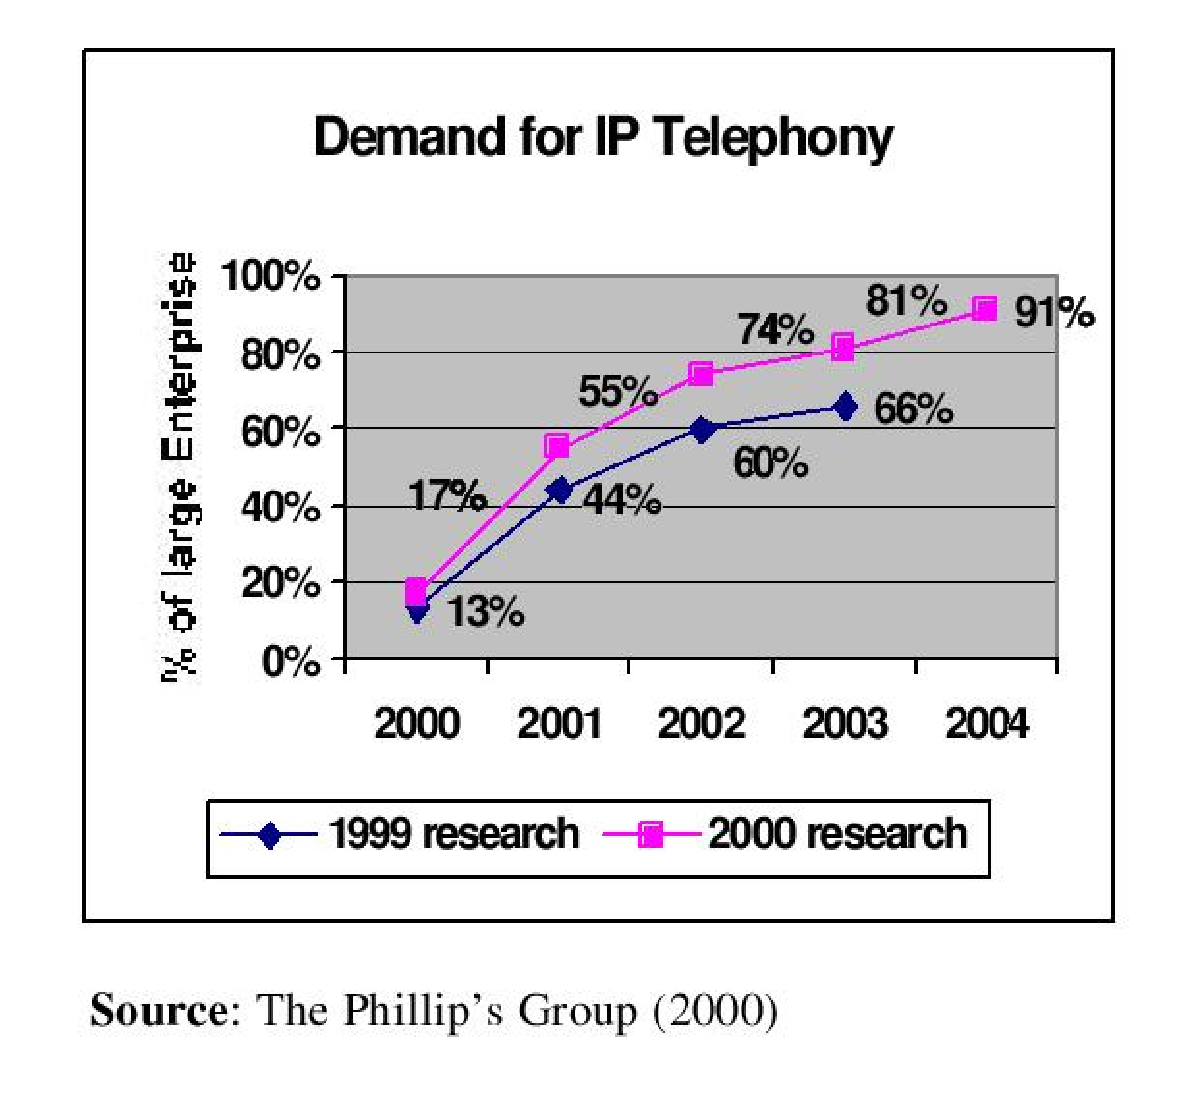
\includegraphics[width=12cm, height=10cm] {espectativas_voip.eps}
\caption{Espectativas de para el crecimiento de VoIP.}
\label{fig:espectativas_voip}
\end{figure}

Sin embargo, queda todav�a por clarificar en este mercado el papel de las grandes operadoras de telefon�a ``tradicional'': la transmisi�n de voz sobre redes \emph{IP} supone una seria amenaza para su modelo de negocio, y no hay que olvidar que generalmente son ellas las que proporcionan la conectividad a Internet. Parece por lo tanto poco factible que no usen su posici�n de fuerza para impedir el uso de estos servicios.

\subsection{Conclusiones}

La viabilidad y el an�lisis de riesgo est�n relacionados de muchas maneras. Si el riesgo del proyecto es alto la viabilidad de producir software de calidad se reduce. Las conclusiones extra�das se agrupan en tres partes diferenciadas:

\begin{description}
	\item[Viabilidad econ�mica.] En el caso de este proyecto no es necesario un estudio de viabilidad econ�mica ya que los beneficios ni la justificaci�n econ�mica no existe. Se trata de un proyecto hecho con software libre y para ser ``open source''.
	\item[Viabilidad t�cnica.] La viabilidad tecnol�gica es frecuentemente el �rea m�s dif�cil de valorar en esta etapa del proceso. Es esencial que el proceso de an�lisis y definici�n se realice en paralelo con una valoraci�n de la viabilidad t�cnica. De todas formas, en este caso la viabilidad t�cnica es positiva, puesto que el riesgo t�cnico es bajo, como lo demuestra la existencia de proyectos similares, que m�s adelante ser�n comentados en la seccion de \emph{Antecedentes}.
	\item[Viabilidad legal.] No se esperan problemas legales, aunque la existencia de patentes de software en algunos pa�ses, junto con las restricciones a la implementaci�n de determinados algoritmos de cifrado en otros, puede limitar el uso del software. Los problemas relacionados con sistemas cifrados pueden evitarse haciendo varias versiones del software y/o con compilaci�n condicional.
\end{description}

\section{Antecedentes}

En esta secci�n se explicar�n las principales soluciones que se han dado al problema de la telefon�a sobre \emph{IP} en general. Luego se comparar� el proyecto con otros de prop�sito similar que existen en este momento.

\subsection{Estado del arte}

Debido a la filosof�a de Linux, y en general de todo el software libre, tardaron en aparecer aplicaciones que usaran t�cnicas \emph{VoIP} para transmitir audio. La filosof�a ``open source'' choca frontalmente con las patentes de software y los est�ndares cerrados. Hasta antes del 2000, s�lo exist�a un proyecto de \emph{VoIP} que funcionaba en Linux con unas caracter�sticas aceptables, se trataba de \textbf{Speak Freely}. Esta situaci�n estaba provocada porque s�lo hab�a un est�ndar disponible, el \emph{H.323} de la \emph{ITU}, y para acceder a la descripci�n del \emph{H.323} es necesario abonar una cantidad de dinero a la \emph{ITU-T}. Otros inconvenientes de \emph{H.323} son: complejidad -est� formado por otros protocolos-; es pr�cticamente cerrado y algunos c�decs de compresi�n de voz que usa son propietarios. A finales del 2000, el grupo \emph{MMUSIC} del \emph{IETF}, estandariz� un nuevo protocolo, el \emph{SIP} (Session Initiation Protocol). Este protocolo, a diferencia del anterior es mucho m�s ligero; su est�ndar es abierto -est� disponible en Internet- y todav�a se encuentra en estado de desarrollo y revisi�n. \emph{SIP} Es un protocolo muy simple y f�cil de implementar y a diferencia de \emph{H.323}, que define todo el proceso de comunicaci�n de audio, \emph{SIP}, s�lo define como se debe iniciar la sesi�n; la transmisi�n de audio es independiente de \emph{SIP}. \\

A partir de la publicaci�n de \emph{SIP} (primavera 2001) empezaron a surgir muchos proyectos de \emph{VoIp} para Linux, FreeBsd, etc. que apostaron decididamente por \emph{SIP} frente a \emph{H.323}, esa es la raz�n por la que (casi) todos los proyectos ``open source'' emplean SIP junto con RTP. \\

RTP es el otro protocolo en liza. Es un protocolo que se emplea para transportar el audio comprimido a trav�s de una red (\emph{IP}), pero, para conocer las caracter�stas -formato de compresi�n, puertos de recepci�n y env�o, etc.- de esa transmisi�n es nesario \emph{SIP} � \emph{H.323}. Por esta raz�n, antes del a�o 2000, era muy complicado usar \textbf{Speak Freely}, ya que no usaba ninguno de estos dos protocolos. Para iniciar una conversaci�n con \textbf{Speak Freely}, ambos usuarios deb�an conocer y configurar los par�metros de RTP y del audio comprimido. \\

En el cap�tulo \ref{chp:analisis_tecnologico} se detallar� una introducci�n \emph{H.323}, \emph{SIP} y \emph{RTP} y se analizar�n todas sus caracter�sticas.

\subsection{Proyectos similares}

Los m�s importantes se detallan a continuaci�n. Las caracter�sticas de cada uno de ellos est�n analizadas a fecha de Junio de 2003.

\paragraph{Linphone,}creaci�n de Simon Morlat, tiene licencia \emph{GPL} y permite realizar de manera f�cil y eficiente llamadas de voz sobre \emph{IP} desde el entorno de \emph{GNOME} a trav�s de Internet o redes locales entre estaciones GNU/Linux y hacia otros soft-phones compatibles con SIP.
Estas son las caracter�sticas de \textbf{linphone}:
	\begin{itemize}
		\item Desarrollado para linux -aunque no se descarta el funcionamiento en otras plataformas \emph{Unix}- y usando el entorno \emph{Gnome}, pero puede ejecutarse en \emph{KDE}, adem�s, a partir de la version 0.9.0, est� disponible una versi�n para consola llamada {\it \textbf{linphonec}}.
		\item Interfaz gr�fica f�cil de usar, como un tel�fono celular, con s�lo dos botones, ya que incorpora una agenda en la que guardar los contactos.
		\item Incluye una gran variedad de codecs compresores de audio: ADPCM. GSM, Speex, etc. Estos codecs est�n integrados en el c�digo del programa.
		\item Utiliza el protocolo \emph{SIP}. \emph{SIP} es un Protocolo de Inicio de Sesion (Session Initiation Protocol) que est� estandarizado por la \emph{IETF}\footnote{Internet Engineering Task Force, define los est�ndares de Internet (http://www.ietf.org)}.
		\item Es software libre, liberado bajo los t�rminos de la \emph{GPL}.
	\end{itemize}

	El software est� integramente programado en C, con t�cnicas de OO (Orientaci�n a Objetos). Tiene una librer�a independiente llamada \emph{oRTP} (Open RTP) que implementa el protocolo RTP, desarrollada usando POO y paralelamente al programa \textbf{linphone}. Sin embargo todav�a no soporta cifrado de RTP ni el protocolo RTCP. La p�gina web del proyecto es {\it http:www.linphone.org}. \\

\paragraph{Speak Freely.}Tal vez sea uno de los primeros programas creados para este menester -iniciado en 1991 por John Walker, fundador de \emph{Autodesk}- es, por ello, uno de los m�s populares. Existen versiones para sistemas \emph{Unix} -tanto \emph{System V} como \emph{BSD}- y Windows. Las caracter�sticas m�s destacables de \textbf{Speak Freely} son:
	\begin{itemize}
		\item Multiplataforma, existen versiones tanto para sistemas \emph{Unix} como \emph{Windows}.
		\item Interoperabilidad con ICQ, un servicio de mensajer�a instant�nea.
		\item Modo de conferencia, que permite charlar con varias personas a la vez, sin necesidad de estar en redes \emph{multicasting}.
		\item Permite grabar mensajes de voz que informen a la persona llamante de que no est� disponible.
		\item Soporta cifrado de las sesiones. Implementa varios algoritmos de cifrado: DES, IDEA, PGP, Blowfish, etc.
		\item Aparte de \emph{RTP}, implementa el protocolo \emph{VAT} (Visual Audio Tool), un protocolo muy simple de streaming de audio en tiempo real creado en \emph{Lawrence Berkeley Laboratory} (http//:www.lbl.org). Este protocolo no est� estandarizado por ninguna organizaci�n.

		\item Soporta estos codecs compresores de audio: DVI4, GSM, L16, LPC, PCMA y PCMU. Est�n integrados dentro del programa.
		\item Es software libre, liberado bajo los t�rminos de la \emph{GPL}.
	\end{itemize}

Las principales caracter�sticas de este programa son ser multiplataforma -la versi�n 6.0 puede ser ejecutada en plataformas de 16 bits como \emph{OS/2 Warp} y tiene total interoperabilidad con las restantes, anteriores y posteriores-  y la posibilidad de tener varias sesiones con distintos usuarios (modo de conferencia). La versi�n actual (7.0) est� programada en \emph{C}, si bien, los desarrolladores planear reescribir el c�digo en \emph{C++} para la version 8.0 y futuras. Tambi�n existen versiones sin algoritmos criptogr�ficos, por restricciones legales en algunos pa�ses. M�s informaci�n en {\it http://www.speakfreely.org}. \\
	
\paragraph{RAT - Robust Audio Tool.}Como su propio nombre indica es, probablemente el programa m�s robusto para conferencia de audio.  Las caracter�sticas m�s importantes son:
\begin{itemize}
		\item Multiplataforma, FreeBSD, HP-UX, IRIX, Linux, NetBSD, Solaris, SunOS y Windows 95/NT.
		\item Incorpora t�cnicas de control de detecci�n de voz, detecci�n de ruido, etc.
		\item Multiconferencia, que permite charlar con un grupo de personas, pero necesita redes \emph{multicasting}.
		\item Completamente compatible con el est�ndar RTP/RTCP, puede incluso enviar audio redundante para contrarestar p�rdidas de paquetes.
		\item Soporta cifrado de sesiones RTP/RTCP con DES.
		\item Soporta estos codecs compresores de audio: GSM, ADPCM (G.726), G.711 y LPC. Est�n integrados dentro del programa.
		\item Es software libre, liberado bajo los t�rminos de la \emph{GPL}.
\end{itemize}

Este programa se diferencia de los anteriores en que soporta el protocolo RTP/RTCP �ntegramente. Tambi�n tiene varios sistemas de reparaci�n de audio, lo que permite que aunque se pierdan paquetes de audio el usuario no note esas p�rdidas. Las estrategias de reparaci�n de audio son:
\begin{description}
		\item[Envio redundante de audio.] Cada vez que se envia un paquete, se aprobecha para enviar los $n$ anteriores, conjuntamente. De esta forma, si se pierde alg�n paquete, s�lo es necesario esperar al siguiente, el cual contendr� el audio para el instante actual y para $n$ instantes anteriores. El problema se produce cuando se pierden $n$ paquetes o m�s, no existen posibilidades de reparaci�n. El inconveniente de este sistema es que multiplica por $n$ el ancho de banda requerido y, en el peor de los casos, se puede producir un retardo de varios segundos en el audio recibido.
		\item[Entrelazado de audio] Una vez formado un paquete, se divide en $n$ trozos, forma un nuevo paquete compuesto por $n$ trozos ordenados secuencialmente de los paquetes originales, y se envia el paquete compuesto. Para recomponer un paquete, es necesario esperar la llegada de $n$. La ventaja de este sistema es que no aumenta el ancho de banda consumido, pero la conversaci�n sufre un retardo constante de varios segundos, debido a la necesidad de esperar a $n$ paquetes. Si se pierde un paquete el usuario no notar� nada, ya que afectar� m�nimamente a los $n$ paquetes sucesivos.
\end{description}
Esta aplicaci�n tambi�n puede hacer streaming de audio. M�s informaci�n en {\it http://www-mice.cs.ucl.ac.uk/multimedia/software/rat}.




\capitulo{An�lisis tecnol�gico}
\label{chp:analisis_tecnologico}
%\newpage
%\thispagestyle{empty}
\minitoc
\newpage

Este cap�tulo sirve de peque�a introducci�n t�cnica de las distintas tecnolog�as empleadas en el desarrollo de este proyecto.

\section{Tratamiento del sonido}

Esta secci�n pretende introducir al lector una serie de conocimientos b�sicos acerca de la naturaleza del sonido. En un principio se presentan una  serie de conceptos f�sicos claves para enterder su naturaleza, propagaci�n, percepci�n por el o�do humano. M�s adelante se aborda el procesado digital del sonido y su tratamiento desde el punto de vista del procesamiento de se�ales, esto es, como el sonido es captado por un dispositivo digital como un muestreador DSP para ser tratado y procesado. La terminolg�a empleada en esta secci�n es clave para enterder cap�tulos posteriores.

\subsection{Ac�stica}

Se entiende por ac�stica la parte de la f�sica que trata del sonido y de todo lo que a �l se refiere.

\subsubsection{Sonido}

Desde el punto de vista f�sico el sonido es una vibraci�n mec�nica en un gas, l�quido o medio s�lido. La propiedad el�stica del medio permite al sonido propagarse en forma de onda desde la fuente, algo parecido a las ondas que se generan en un charco al arrojar una piedra. Cada vez que un objeto vibra, una peque�a porci�n de energ�a se pierde en forma de sonido, o expresado de otro modo, la vibraci�n provoca un transvase de energ�a al medio -normalmente el aire- que da lugar al sonido. \\

El sonido se propaga en el aire en forma de variaci�n de presi�n. Un altavoz, por ejemplo, transmite las variaciones de presi�n al aire y s�lo esta variaci�n se mueve, no el aire; en la comparaci�n del charco mencionada antes, las ondas se desplazan por el agua, mientras que �sta permanece en el mismo lugar, pero oscilando verticalmente. En el aire las ondas de sonido se propagan a 340 metros por segundo en condiciones normales. En la figura ~\ref{fig:vibracion_fluido} se muestra la propagaci�n de la onda en un medio que podr�a ser el aire.

\begin{figure}[hbt]
\centering
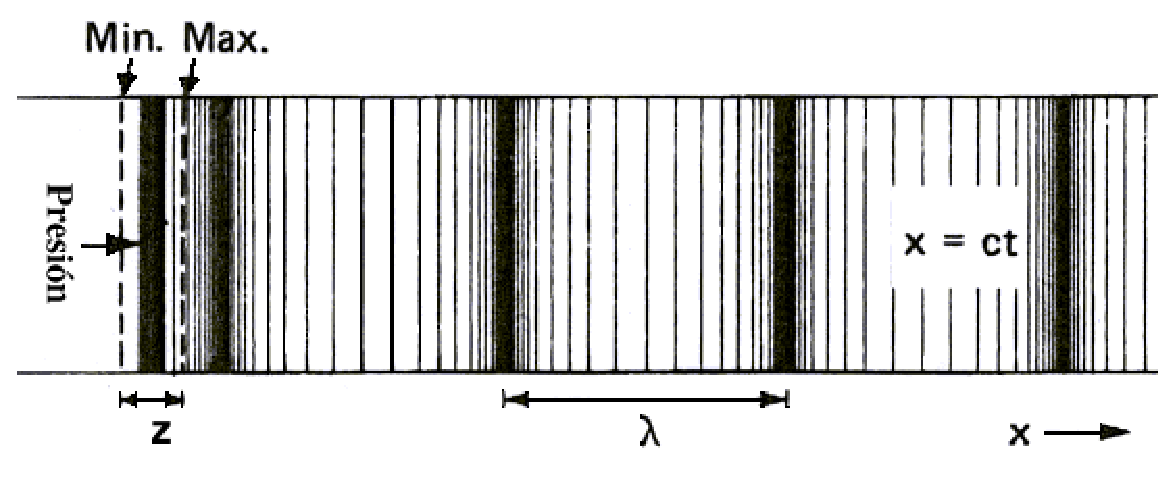
\includegraphics[width=10cm, height=5cm] {vibracion_fluido.eps}
\caption{Transmisi�n de la vibraci�n en un fluido}
\label{fig:vibracion_fluido}
\end{figure}

El par�metro $Z$ es la amplitud de onda, es le valor m�ximo que puede alcanzar. El par�metro $T_{0}$ es el per�odo, se expresa en segundos; $T_{0}$ es igual al inverso de la frecuencia $F$. La frecuencia se expresa en \emph{Hercios} ($Hz$). \\

A continuaci�n se va a definir un modelo matem�tico que describe la naturaleza del sonido. Cualquier sonido gen�rico se puede formar a partir de una suma de movimientos arm�nicos simples, por ello se van a definir las caracter�sticas del movimiento arm�nico. Si se representa la figura ~\ref{fig:vibracion_fluido} como una onda se obtiene la figura ~\ref{fig:forma_onda}
\begin{figure}[hbt]
\centering
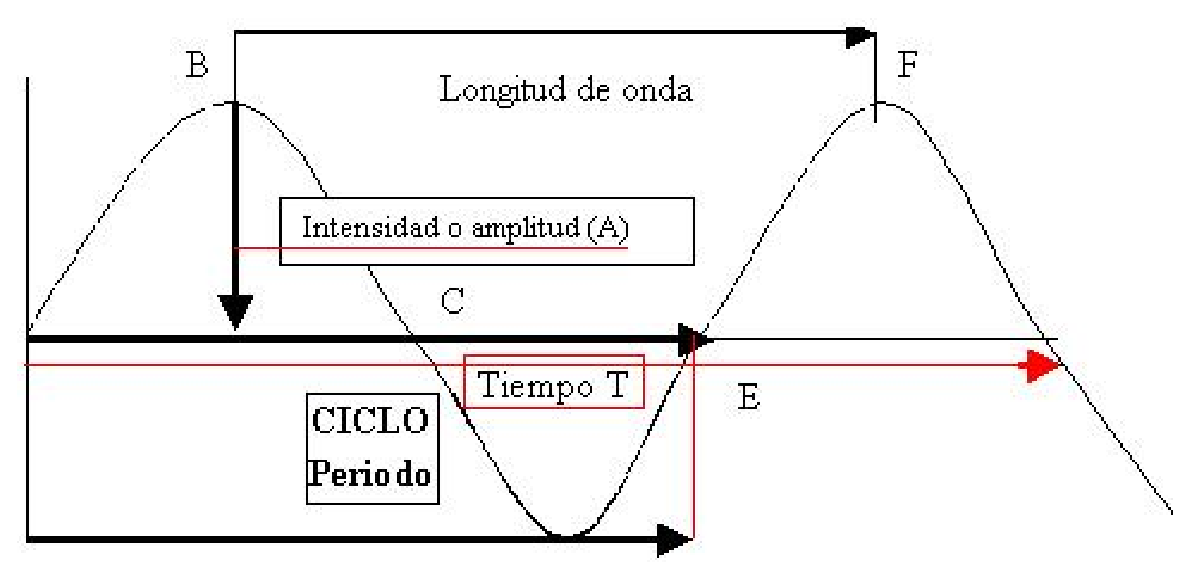
\includegraphics[width=10cm, height=5cm]{forma_onda.eps}
\caption{Movimiento arm�nico simple}
\label{fig:forma_onda}
\end{figure}

Como toda onda se puede considerar como superposici�n de ondas sinusoidales de frecuencia, amplitud y fase correspondientes (\emph{Teorema de Fourier}), un sonido complejo se puede descomponer como una suma de arm�nicos simples de distinta frecuencia. \\

Las ondas sonoras capaces de ser detectadas por el o�do humano van desde 20 Hz (umbral inferior) a 20000 Hz (umbral superior). Por debajo de 20 Hz est�n los infrasonidos (mareas, ondas s�smicas) y por encima de 20000 Hz, los ultrasonidos (como el sonar, de baja energ�a, y las vibraciones de las redes cristalinas (cuarzo), de alta energ�a. \\

El ruido es un sonido audible no armonioso. Procede de ondas no peri�dicas. Una nota musical es un sonido agradable; procede de ondas peri�dicas. El sonido o nota fundamental es la v�braci�n cuya frecuencia $F_{0}$, es la m�s baja que se puede obtener en la flauta aguda (caramillo). Un arm�nico es una nota cuya frecuencia es un m�ltiplo entero de $F_{0}$. \\

Las notas o sonidos musicales se caracterizan por la intensidad, el tono y el timbre. La intensidad de un sonido depende de la mayor o menor amplitud de la onda, ya que la energ�a de la misma es funci�n del cuadrado de la amplitud. La audici�n est� unida a la intensidad de la onda sonora. Para cada frecuencia hay una intensidad m�nima (umbral de audici�n) por debajo de la cual no se oye; y una intensidad m�xima que produce sensaci�n de dolor (umbral doloroso). El nivel de intensidad sonoro, se mide en decibelios ($dB$) que se explicaran m�s adelante. El tono de un sonido depende de su frecuencia. Los tonos agudos tienen mayor frecuencia que los graves. De la relaci�n: $f = v/l$ se deduce que a mayor longitud de onda, menor frecuencia, y viceversa. El timbre depende de los arm�nicos que acompa�an a los sonidos; como �stos var�an con los instrumentos, por el timbre se distingue una nota dada por diferentes instrumentos. \\

\subsubsection{Amplitud}

La medida de la amplitud de una onda es importante porque informa de la fuerza, o cantidad de energ�a, de una onda, que se traduce en la intensidad de lo que o�mos, su unidad de medida es el decibelio. Un decibelio, abreviado como dB, es una unidad de medida de la fuerza de la se�al y es �til en la comparaci�n de la intensidad de dos sonidos. La sensibilidad del o�do humano es extraordinaria, con un rango din�mico o variaci�n en intensidad muy amplio. La mayor�a de los o�dos humanos pueden capturar el sonido del murmullo de una hoja y, despu�s de haberse sometido a ruidos explosivos como los de un avi�n, siguen funcionando. Lo que es sorprendente es que la fuerza de la explosi�n en un avi�n es al menos 10 millones de veces mayor que el murmullo que una hoja produce con el viento. \\

Seg�n la {\it ley de Weber-Fechner}, el efecto sobre el o�do de un cambio de intensidad depende de la intensidad que precede al cambio, por ello el o�do necesita un porcentaje elevado de variaciones en la fuerza de un sonido para detectar un cambio en la intensidad percibida. Una forma simple de comprender esto es comenzar con una nota de determinada intensidad, por ejemplo 10 unidades, incrementarla luego a 100 y despu�s a 1000 unidades. Estos dos cambios los interpretar�a el o�do como id�nticos en potencia, puesto que la proporci�n de $100/10$ es igual a $1000/100$. Otro modo de expresar esto es escribir los valores de las intensidades en potencias de diez: $10^{1}$, $10^{2}$, $10^{3}$ y se aprecia que los cambios iguales en potencia vienen dados por cambios iguales al logaritmo de la intensidad. El o�do tiene una respuesta logar�tmica y en mediciones de ac�stica se emplea una unidad llamada {\it belio}, abreviado {\it B} . Si la intensidad inicial $I_{0}$ se incrementa hasta un nuevo valor $I_{1}$ se tiene:

\[
belios = log_{10} \left( \frac{ I_{1}} {I_{0} } \right)
\]
\\

En la pr�ctica, el belio es demasiado grande y por ello se emplea el {\it decibelio} ({\it dB}). La relaci�n en decibelios ser� entonces:

\begin{equation}
dB = 10 \cdot log_{10} \left( \frac{ I_{1}} {I_{0} } \right)  \label{eq:ecuacion1_decibelios}
\end{equation}

donde $I_{0}$, es la intensidad inferior de audici�n que se toma como punto de referencia y en el aire vale: $I =10^{-12} W_{m} ^{-2}$. As� un sonido cuya intensidad sea 1000 veces superior a $I_{0}$ tiene de nivel de:  $10 log (10^{3} 10^{-22}/10^{-12}) = 30  dB$. \\

Los logaritmos representan un recurso muy �til de c�lculo, y a esto se debe que el decibelio se use universalmente en ingenier�a electr�nica para comparar dos potencias el�ctricas. As�, por ejemplo, si la potencia de entrada de un amplificador es $W_{0}$ y la de salida $W_{1}$, la amplificaci�n en decibelios ser�:

\[
A = 10 \cdot log_{10} \left( \frac{W_{1}}{W_{0}} \right)
\]

En ac�stica se suele tratar con mayor frecuencia con presiones que con intensidades, y con dos presiones, la relaci�n en decibelios es: 

\begin{equation}
dB = 20 \cdot log_{10} \left( \frac{P_{1}}{P_{0}} \right)  \label{eq:ecuacion_decibelios}
\end{equation}

donde $P_{0}$ es la presi�n inicial y $P_{1}$ la presi�n con la que se quiere relacionar. Esta relaci�n se obtiene a partir de la f�rmula ~\ref{eq:ecuacion1_decibelios} y considerando que $intensidad = f (presion^{2})$ :
\begin{eqnarray}
dB & = & 10 \cdot log_{10} \left( \frac{ P_{1}^{2} } { P_{0}^{2} } \right)  \nonumber \\
& = & 20 \cdot log_{10} \left( \frac{ P_{1} } { P_{0} } \right)
\end{eqnarray}

\begin{figure}[htb]
\centering
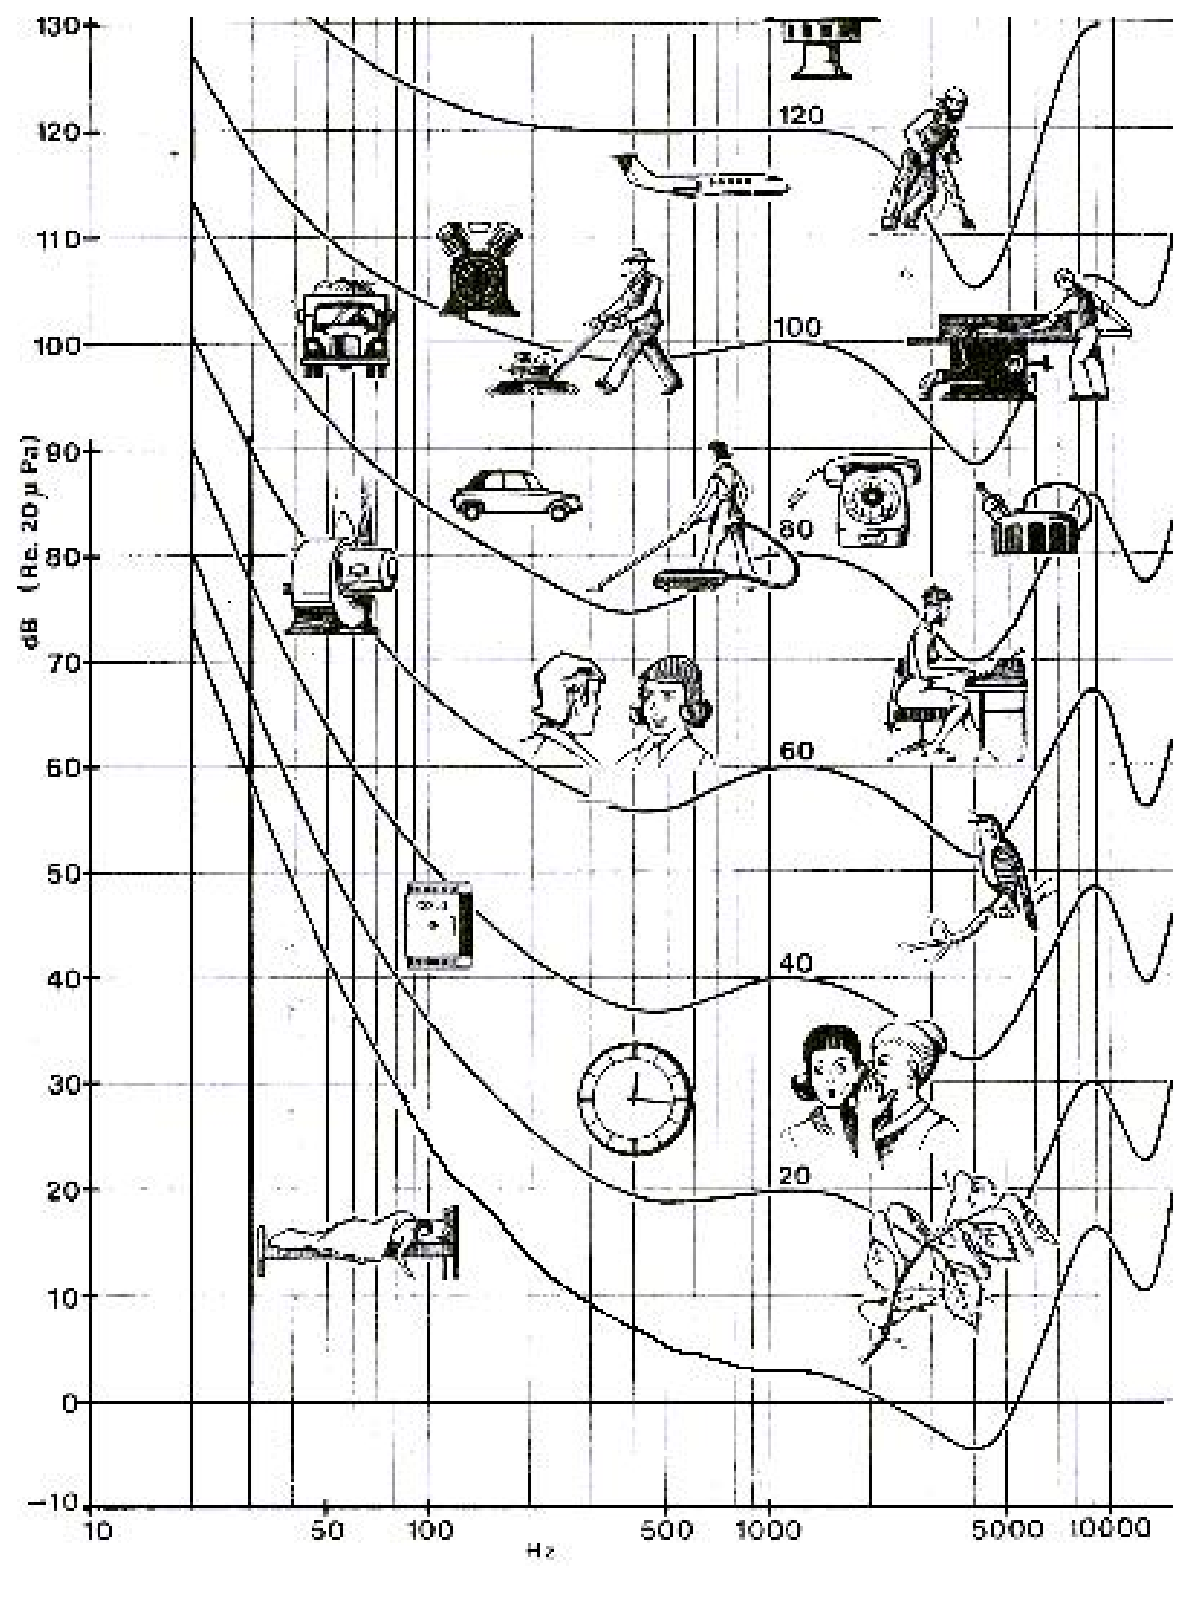
\includegraphics[width=9cm, height=11cm] {db_sources.eps}
\caption{dB de varias fuentes de sonido}
\label{fig:dB_sources}
\end{figure}

En el aspecto pr�ctico de la amplitud, un incremento de s�lo 3 dB duplica la intensidad de un sonido. Por ejemplo, un sonido con 86 dB tiene, el doble de fuerza que un sonido con 83 dB y cuatro veces m�s que un sonido con 80 dB. Desde la perspectiva de nuestra percepci�n de la intensidad, un incremento de 3 dB, que da lugar a que se duplique la fuerza, provoca que el sonido se perciba s�lo ligeramente m�s alto. Es necesario un aumento en 10 dB para que nuestros o�dos perciban un sonido con el doble de intensidad.  La figura ~\ref{fig:dB_sources} muestra el nivel en $dB$ de varias fuentes de sonido usuales.

\subsubsection{Rango din�mico}

El rango din�mico es el variaci�n de frecuencias que puede alcanzar o recorre una se�al de audio. Es una caracter�stica que influye notablemente en la calidad de los sonidos grabados. El rango din�mico de un sonido reproducido nunca es comparable al real. La raz�n principal es que un sistema -anal�gico o digital- no puede duplicar el rango din�mico completo de, por ejemplo, una orquesta o de un concierto de rock. Una orquesta puede alcanzar los 110 $dB$ en su climax y en el punto m�s suave bajar hasta los 30 $dB$, dando lugar a un rango din�mico de 80 $dB$. Este rango es superior al rango din�mico de un sistema est�reo t�pico y, de hecho, superior a la capacidad de grabaci�n de medios tales como un disco de vinilo y una cinta de audio. El programa, por ejemplo, tiene un rango dinamico (interno) de 96 $dB$, ya que trabaja con audio en formato 16 bits y partiendo de la ecuaci�n de c�lculo de $dB$  ~\ref{eq:ecuacion_decibelios}, se  obtiene :
\[
Rango \: dinamico\: =  20 \cdot log_{10} \left( R_{\Delta} \right) = 20 log_{10} ( 2^{16} ) = 96\, dB
\]
En la siguiente lista se muestra rango din�mico varios sistemas de almacenamiento de audio:
\begin{itemize}
\item Disco de vinilo: 65 $dB$
\item Cinta magnetof�nica: 55 $dB$
\item Cd-Audio (16 bits): 96 $dB$
\item Muestreo 8 bits: 48 $dB$
\end{itemize} 

\subsubsection{Ancho de banda}

Existe una medida est�ndar para definir el ancho de banda: el rango de frecuencias sobre el que la amplitud de la se�al no difiere del promedio en m�s de 3 dB, es decir la diferencia de las frecuencias en la que se produce una ca�da de 3 dB, ya es el punto donde su amplitud cay� a la mitad, y �ste es el m�nimo cambio en la fuerza de la se�al que puede ser percibido como un cambio real en la intensidad por la mayor�a de los o�dos. \\

A menudo el ancho de banda se simboliza mediante un �nico n�mero cuando la frecuencia baja est� bastante pr�xima a cero. Por ejemplo, el ancho de banda de una voz femenina se sit�a en torno a los 9 kHz, aunque realmente puede estar en el rango que va desde los 200 Hz hasta los 9 kHz. \\

Es importante tener en cuenta que el ancho de banda de un sistema de sonido depende del enlace m�s d�bil del canal, que normalmente no es la tarjeta de sonido. La calidad del sonido producido por el PC refleja el esfuerzo de muchos componentes, y la salida no ser� mejor que la interpretaci�n del miembro menos capacitado de un grupo. En el caso del sistema de sonido del ordenador, una se�al debe pasar por muchas fases de transformaci�n de audio y por diferentes dispositivos. Por ejemplo, el sonido grabado mediante un micr�fono y que luego es reproducido. La tarjeta de sonido transforma el sonido recogido del micr�fono en una se�al el�ctrica que, posteriormente, se transforma en audio digital y se almacena en disco. El audio digital del disco es transformado de nuevo en una se�al el�ctrica y reproducido a trav�s de los cascos o de los altavoces. El ancho de banda efectivo del sistema de sonido est� limitado por el dispositivo con el ancho de banda m�s estrecho de todos los dispositivos que procesan el sonido. El enlace m�s d�bil en grabaci�n suele ser el micr�fono, que tiene probablemente un ancho de banda aproximadamente de 12 kHz. 

\subsection{Psicoac�stica}

El o�do humano percibe un rango de frecuencias entre 20 Hz. y 20 Khz. En primer lugar, la sensibilidad es mayor en la zona alrededor de los 2-4 Khz., de forma que el sonido resulta m�s dif�cilmente audible cuanto m�s cercano a los extremos de la escala. En segundo lugar est� el enmascaramiento, cuyas propiedades utilizan exhaustivamente los algoritmos m�s interesantes: cuando la componente a cierta frecuencia de una se�al tiene una energ�a elevada, el o�do no puede percibir componentes de menor energ�a en frecuencias cercanas, tanto inferiores como superiores. A una cierta distancia de la frecuencia enmascaradora, el efecto se reduce tanto que resulta despreciable; el rango de frecuencias en las que se produce el fen�meno se denomina banda cr�tica. Las componentes que pertenecen a la misma banda cr�tica se influyen mutuamente y no afectan, ni se ven afectadas, por las que aparecen fuera de ella. La amplitud de la banda cr�tica depende de la frecuencia y viene dada por unos determinados datos que demuestran que es mayor con la frecuencia. Hay que se�alar que estos datos se obtienen por experimentos psicoac�sticos, que se realizan con expertos entrenados en percepci�n sonora, dando origen con sus impresiones a los modelos psicoac�sticos. \\

Lo descrito es el llamado enmascaramiento simult�neo o en frecuencia. Existe, asimismo, el denominado enmascaramiento asimult�neo o en el tiempo, as� como otros fen�menos de la audici�n que no resultan relevantes en este punto. La idea es que ciertas componentes en frecuencia de la se�al admiten un mayor ruido del que generalmente considerar�amos tolerable y, por tanto, requieren menos bits para ser codificadas si se dota al codificador de los algoritmos adecuados para resolver m�scaras. \\

Otra consideraci�n importante en las comunicaciones de audio es la calidad de la transmisi�n.
Si la calidad es muy buena y se usan t�cnicas de transmisi�n discontin�a o DT (Discontinous Transmission) apoyadas por VAD (Voice Activity Detection o detecci�n de voz) provoca que los interlocutores tengan a veces la sensaci�n de que se ha perdido la comunicaci�n y aparecan expresiones del tipo ``sigues ah�'', ``me escuchas'', etc. Esto se soluciona generando lo que se conoce como \emph{ruido de comfort} mediante el sistema CNG (Comfort Noise Generation). El ruido de comfort se genera en el propio terminal, es un enga�o del sistema, y consiste en generar un ligero ruido gausiano de fondo, pero sin entorpecer la comunicaci�n.

\subsection{Modulaci�n de audio}

La tecnolog�a digital es m�s avanzada y ofrece mayores posibilidades, menor sensibilidad al ruido en la transmisi�n y capacidad de incluir c�digos de protecci�n frente a errores, as� como cifrado. Con los mecanismos de decodificaci�n adecuados, adem�s, se pueden tratar simult�neamente se�ales de diferentes tipos transmitidas por un mismo canal. La desventaja principal de la se�al digital es que requiere un ancho de banda mucho mayor que el de la se�al anal�gica, de ah� que se realice un estudio en lo referente a la compresi�n de datos. \\

El proceso de digitalizaci�n se compone de dos fases: muestreo y cuantizaci�n. En el muestreo se divide el eje del tiempo en segmentos discretos: la frecuencia de muestreo ser� la inversa del tiempo que medie entre una medida y la siguiente. En estos momentos se realiza la cuantizaci�n, que, en su forma m�s sencilla, consiste simplemente en medir el valor de la se�al en amplitud y guardarlo. El teorema de Nyquist garantiza que la frecuencia necesaria para muestrear una se�al que tiene sus componentes m�s altas a una frecuencia dada $f$ es como m�nimo $2f$. Por tanto, siendo el rango superior de la audici�n humana en torno a los 20 Khz, la frecuencia que garantiza un muestreo adecuado para cualquier sonido audible ser� de unos 40 Khz. Concretamente, para obtener sonido de alta calidad se utilizan frecuencias de 44'1 Khz (CD Audio). Otros valores t�picos son subm�ltiplos de la primera, 22 y 11 Khz. Seg�n la naturaleza de la aplicaci�n, por supuesto, las frecuencias adecuadas pueden ser muy inferiores, de tal manera que el proceso de la voz acostumbra a realizarse a una frecuencia de entre 6 y 20 Khz. En lo referente a la cuantizaci�n, es evidente que cuantos m�s bits se utilicen para la divisi�n del eje de la amplitud, m�s ``fina'' ser� la partici�n y por tanto menor el error al atribuir una amplitud concreta al sonido en cada instante. Por ejemplo, 8 bits ofrecen 256 niveles de cuantizaci�n y 16, 65536. El margen din�mico de la audici�n humana es de unos 100 dB. La divisi�n del eje se puede realizar a intervalos iguales o seg�n una determinada funci�n de densidad, buscando m�s resoluci�n en ciertos tramos si la se�al que se trata tiene m�s componentes en cierta zona de intensidad. \\

 \begin{figure}[hbt]
\centering
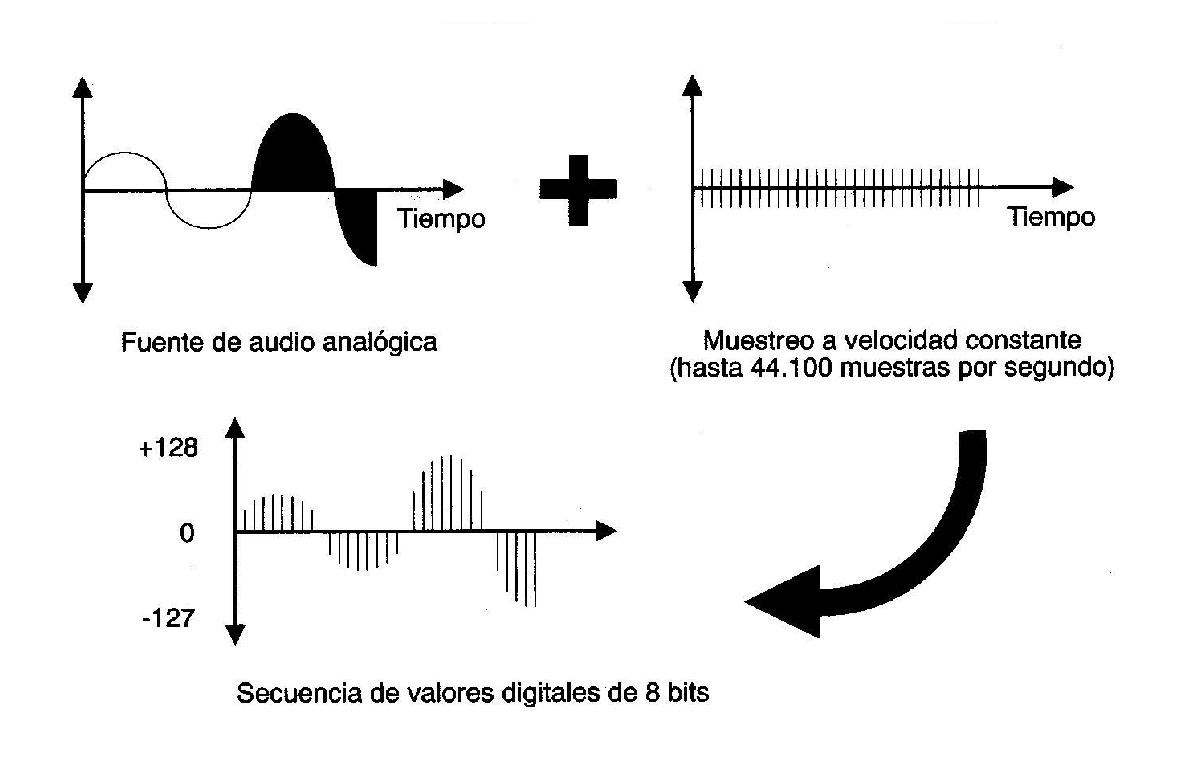
\includegraphics[width=\textwidth, height=9cm] {muestreo.eps}
\caption{Conversi�n Anal�gico-Digital del sonido (ADC)}
\label{fig:modulacion_audio}
\end{figure}

La modulaci�n por impulsos codificados (PCM) es el m�todo m�s com�n de codificar una voz anal�gica en un flujo digital. El proceso de PCM es el siguiente:
\begin{enumerate}
	\item Las formas de onda anal�gicas se pasan por un filtro de frecuencia de voz
para filtrar cualquier cosa que sea mayor de 4000Hz. Siguiendo  el teorema de Nyquist, se necesita muestrear a 8000 muestras por segundo para alcanzar una transmisi�n de voz de buena calidad.
	\item La se�al anal�gica filtrada es luego muestreada a una velocidad de 8000 veces
por segundo. 
	\item Cuando se ha muestreado la forma de onda, �sta se convierte en una onda digital discreta. Esta muestra est� representada por un c�digo que indica la amplitud de la forma de onda en el instante en que se tom� la muestra. La forma de telefon�a de PCM utiliza 8 bits para el c�digo y un m�todo de compresi�n logar�tmico que asigna m�s bits para se�ales de amplitud m�s baja. \\

Si se multiplican las palabras de 8 bits a 8000Hz, se obtienen 64000 bits por segundo (bps). La base para la infraestructura del tel�fono es 64000 bps (64 kbps).
\end{enumerate}

Normalmente, se utilizan dos variaciones b�sicas de PCM de 64 kbps; la ley u, que es la est�ndar usada en EEUU, y la ley a, que es la est�ndar utilizada en Europa. Los dos m�todos son similares en cuanto ambos utilizan la compresi�n logar�tmica para pasar de 12 a 13 bits de calidad PCM lineal en palabras que tienen s�lo 8 btis, pero se diferencian en detalles de compresi�n relativamente peque�os. El m�todo de la ley u tiene una peque�a ventaja sobre el m�todo de la ley a en t�rminos de rendimiento de la relaci�n se�al-ruido de bajo nivel.

\subsection{Compresi�n de audio}

Para comprimir una se�al de audio, se asigna a un rango de niveles un �nico valor de reconstrucci�n. Esto hace m�s f�cil discernir entre niveles de amplitud, reduciendo el efecto del ruido que se pueda a�adir en una transmisi�n o en un proceso de lectura. El precio que hay que pagar es una distorsi�n de la se�al, ya que esta no recupera su amplitud original en todos los puntos, sino un valor pr�ximo. Esta distorsi�n puede verse como ruido a�adido, en una proporci�n que se puede controlar variando el n�mero de niveles de cuantificaci�n: cuantos m�s niveles, menos ruido. \\

Si en una zona del espectro se introduce ruido sin que se oiga, se realiza una cuantificaci�n menos fina (escalones de cuantificaci�n m�s grandes, que se traduce en menos bits), mientras que en las zonas donde el ruido se hace audible, se asigna m�s bits. Es en este punto donde se diferencian unos codificadores de otros. El c�lculo de la cantidad de ruido que se puede admitir es un dato basado en lo que se llama el "Modelo psicoac�stico". Este modelo es completamente experimental, y se realiza promediando la respuesta de muchas personas frente a determinados est�mulos. Un buen modelo permitir� estimar con precisi�n la cantidad de ruido admisible y la banda donde puede introducirse con p�rdidas m�nimas, mientras que las estimaciones de un mal modelo no permitir�n comprimir tanto o con tanta calidad. No obstante, la elecci�n de un modelo u otro puede venir determinada por diferentes factores, como por ejemplo, el coste computacional.

El procedimiento b�sico es el siguiente:

\begin{enumerate}
	\item Crear ventanas con la se�al: tomar muestras durante unos 10 ms (alrededor de 512 muestras). A este intervalo temporal se le denomina ventana de an�lisis.
    \item An�lisis espectral de la ventana: se divide la se�al en subbandas, generalmente unas 32, que suelen distribuirse de manera uniforme en frecuencia. Hay que calcular un umbral de enmascaramiento para cada una de estas bandas.
    \item Generalmente se usa una \emph{TF} (Transformada de Fourier) o mejor una \emph{FFT} (Transformada r�pida de Fourier), pero pueden utilizarse otras transformaciones, como por ejemplo la \emph{DCT} (Transformada Discreta del Coseno). Al aplicar esta transformaci�n, el espectro se divide en bandas de anchura creciente con la frecuencia, lo que simula el comportamiento del o�do, que tiene m�s resoluci�n espectral en baja frecuencia.
    \item C�lculo de los umbrales de enmascaramiento: esta parte puede hacerse de dos formas. La m�s simple, y la que se usa para factores de compresi�n peque�os, es utilizar la energ�a de las subbandas para estimar los umbrales, que es computacionalmente poco costoso. Para elevar los factores de compresi�n, se necesita afinar m�s en la estimaci�n, lo que se hace calculando una FFT de muchos puntos (m�s de 512) o calcular FFT (o MDCT) de cada una de las subbandas. La decisi�n de usar uno u otro m�todo es un compromiso entre prestaciones y coste computacional. 
    \item Cuantificaci�n: seg�n los umbrales de enmascaramiento y la velocidad binaria de salida se realiza la cuantificaci�n de los coeficientes de cada banda con un n�mero determinado de bits.
\end{enumerate} 

Y este es el proceso b�sico. Evidentemente una implementaci�n real debe tener en cuenta muchos otros factores. Tambi�n suele ser frecuente aplicar un algoritmo de compresi�n est�ndar a la salida o alg�n esquema de compactaci�n eficiente de bits para reducir a�n m�s la tasa binaria. 

\subsection{Otras consideraciones}

A continuaci�n se tratan otras consideraciones a tener en cuenta con el tratamiento del audio digital.

\subsubsection{Detecci�n de voz. VAD}

Existen muchas y muy complejas t�cnicas para detectar la voz. Aqu� se va a mostrar la t�cnica mas b�sica de todas. Consiste, b�sicamente, en calcular la media ponderada de la se�al cuando no hay voz, para m�s tarde comparar ese valor promedio con los obtenidos en las muestras actuales. Si superan ese valor se considerar� que la se�al es v�lida -hay voz- en caso contrario se ignorar� la muestra. Hay dos formas para que se pueden usar para este menester:
 
\begin{description}
	\item [C�lculo de la magnitud.] La magnitud se define como la suma del valor absoluto de las muestras que se encuentran en una ventana; se divide por el n�mero de muestras para normalizar los resultados:
	\begin{equation}
	M(i) = \frac{1}{T_{v}} \sum_{k=0}^{T_{v}-1} \mid m(k) \mid
	\end{equation}
siendo $M(i)$ la magnitud de la ventana $i$, $T_{v}$ el tama�o de la ventana y $m(k)$ la muestra de sonido capturada. 
	\item [C�lculo de la energ�a.] Se define como la suma de las muestras al cuadrado; se divide por el n�mero de muestras para normalizar los resultados.
	\begin{equation}
	M(i) = \frac{1}{T_{v}} \sum_{k=0}^{T_{v}-1}  m^{2}(k)
	\end{equation}
siendo $E(i)$ la energ�a de la ventana $i$.
\end{description} 

\subsubsection{Modificaci�n del volumen en el audio digital}
 
Para modificar el volumen, se multiplican todas las muestras por un determinado factor.
si el factor es mayor que uno, se incrementa el volumen, si es menor que uno, se decrementa 
y si es uno el volumen no var�a. \\

Hay que tener en cuenta que, si al multiplicar una muestra por un factor mayor que uno se produce desbordamiento se truncar�n los d�gitos superiores, pero, esa soluci�n no es adecuada; lo correcto es dejar la muestra con el mayor valor  posible. Esto lo se debe implementar mediante codigo espec�fico. Para el caso particular de pretender aumentar el volumen al m�ximo, sin que se produzca saturaci�n, se debe buscar la muestra de mayor valor absoluto y calcular el factor con el que multiplicar para convertir esta  muestra en el mayor valor que permita el rango. Posteriormente hay que multiplicar todas las muestras por ese factor.
                                                                       
\subsubsection{Mezcla de sonidos digitales}

Basta con sumar las muestras de forma ordenada. S�lo hay que tener en cuenta que no se
produzca truncamiento (\emph{clipping}). Para ello, antes de realizar al suma, se multiplica cada sonido por un factor menor que la unidad. Con esta regla se evita la posibilidad de que se produzca un truncamiento, pero en general, el volumen del sonido final es muy bajo, se debe reajustar para que ronde el 90\% del rango permitido. \\

El factor �ptimo -menor que uno- con el que se deben multiplicar todas las muestras a 
mezclar es el inverso del n�mero de fuentes a mezclar, es decir $f = \frac{1}{N_{f}}$,
donde $N_{f}$ es el n�mero de fuentes.

\section{Protocolo de Internet. IP}

Hoy por hoy, el Protocolo de Internet -\emph{IP}, (Internet Protocol) es el protocolo m�s usado en las redes de comunicaciones telem�ticas, por esta raz�n se ha elegido para el desarrollo del proyecto \software . A continuaci�n se expone una breve introduci�n en el funcionamineto de \emph{IP}, resaltando aquellas car�cter�sticas que pueden afectar al rendimiento de �sta aplicaci�n.

\subsection{Introducci�n}

En general una red de comunicaciones se compone de diferentes medios. Es necesario que se garantice la comunicaci�n entre s� de todos los equipos conectados a la red. El nivel de red oculta los detalles del medio, ofreciendo al usuario la imagen de una �nica red, aunque dicha red est� formada por varias redes distintas en medios f�sicos diferentes. As� este nivel se encarga principalmente de la comunicaci�n extremo a extremo y el encaminamiento. IP es un protocolo que se desenvuelve en el nivel de red, nivel 3 de \emph{OSI} (Open Systems Interconection), su funci�n es hacer lo mejor que pueda la entrega de un datagrama al host destino. Las funciones de \emph{IP} son:

\begin{itemize}
	\item Provee una red virtual �nica independiente de los medios f�sicos y protocolos de enlace.
	\item Cada equipo que se conecta debe tener al menos una direcci�n que lo identifica dentro de la red, por lo que provee de un direccionamiento l�gico uniforme independiente de las redes f�sicas.
	\item A�sla a la capa de transporte de la tecnolog�a, topolog�a, etc. de la red.
	\item Se encarga del establecimiento de rutas.
	\item Control de congesti�n dentro de la red.
	\item Adaptaci�n al tama�o de trama del nivel de enlace (\emph{MTU}).
\end{itemize}

 \begin{figure}[hbt]
\centering
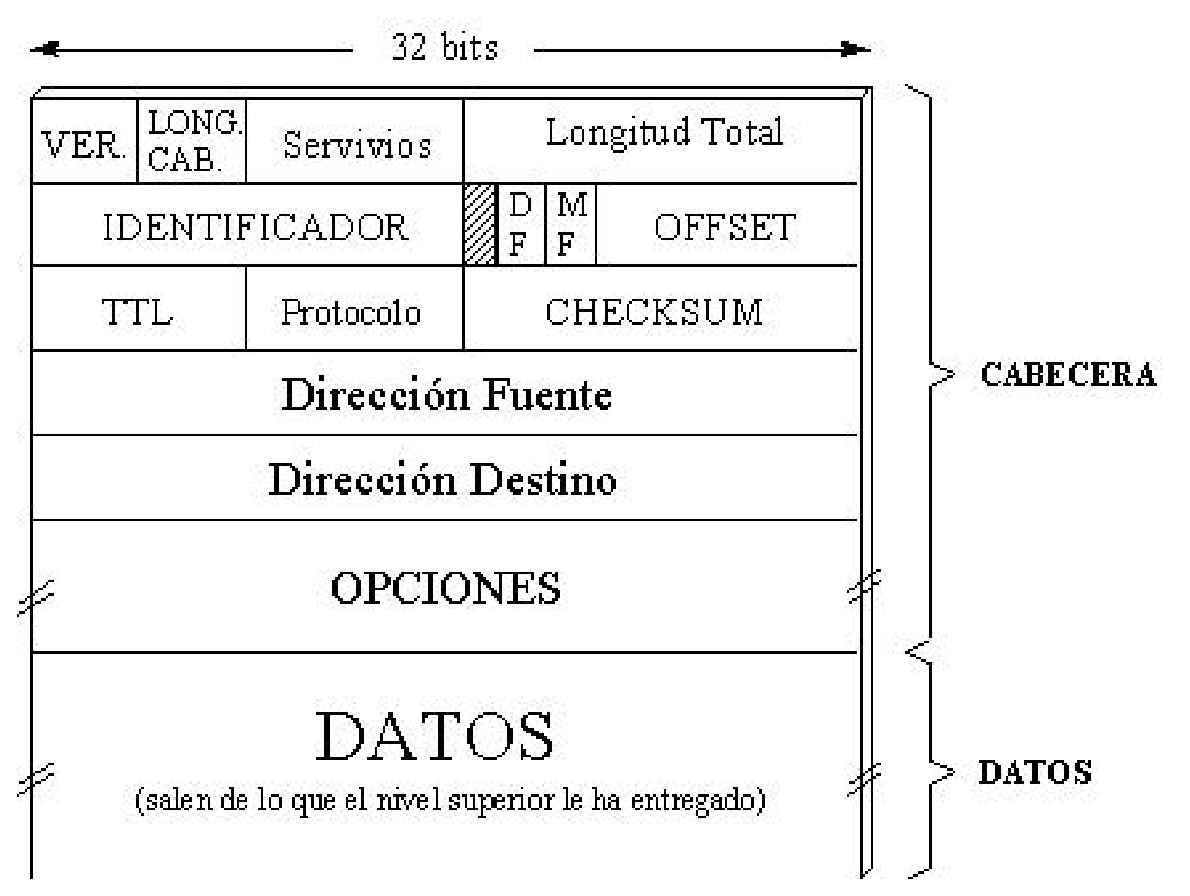
\includegraphics[width=8cm, height=6cm] {cabecera_ip.eps}
\caption{Cabecera de un paquete IP}
\label{fig:ip_header}
\end{figure}

\emph{IP} es un protocolo que proporciona servicios no orientados a conexi�n y no es fiable. Es un protocolo bien intencionado, es decir, un paquete se pierde solamente cuando se dan circustancias excepcionales como un corte en la red. \emph{IP} es el principal protocolo de la capa de red. Este protocolo define la unidad b�sica de transferencia de datos entre el origen y el destino, atravesando toda la red. Adem�s, el software IP es el encargado de elegir la ruta m�s adecuada por la que los datos ser�n enviados. En resumen, se trata de un sistema de entrega de datagramas que tiene las siguientes caracter�sticas:

\begin{itemize}
	\item Es no orientado a conexi�n, cada uno de los paquetes puede seguir rutas distintas entre el origen y el destino, puediendo llegar duplicados o desordenados.
	\item Es no fiable, los paquetes pueden da�arse por errores en los bytes durante la transmisi�n por el medio, perderse o llegar retrasados por un culpa encaminador congestionado, etc.
	\item Cada datagrama es tratado en la red de manera independiente de los dem�s.
	\item El tama�o m�ximo del datagrama es de 65635 bytes, pero se adapta al nivel de enlace.
\end{itemize}

\emph{IP} es un protocolo adaptativo, es decir, en todo momento se realiza una comprobaci�n de la mejor ruta a seguir para el siguiente salto comprobando la tabla de encaminamiento del nodo actual, las entradas de la tabla de encaminamiento pueden cambiar en cualquier momento dependiendo de las condiciones de la red. Por ejemplo si un enlace deja de funcionar se enviaran los datagramas por una ruta diferente, si es que existe. Un cambio en la topolog�a de la red puede hacer que los datagramas se reencaminen autom�ticamente. El encaminamiento adaptativo es la base de la flexibilidad y la robustez de IP. Tambi�n utiliza, t�cnicas de fragmentaci�n y reensamblado junto con temporizadores que permiten encaminar los datagramas a trav�s de encaminadores congestionados o pasar de redes con grandes prestaciones a redes peque�as y de baja calidad de tr�fico. Esto hace posible que un datagrama de IP viaje pasando por una gran variedad de tecnolog�as de comunicaci�n que van desde las redes de telefon�a b�sica hasta los enlaces dedicados por sat�lite o fibra �ptica y viceversa. \\

El funcionamiento de IP se basa en un identificador de 32 bits (direcci�n IP) de un sistema (interfaz). La direcci�n ip est� vinculada a un punto de acceso al servicio, es decir, una direcci�n identifica de forma �nica a un punto de acceso remoto con el cual comunicar. Esto es lo que posibilita el encaminamiento, la direcci�n es �nica en el contexto en que est� siendo utilizada -la red-, ya que identifica perfectamente al destino. Para explicar el tema de manera superficial, IP no necesita conocer la ruta completa que lo llevara a la red destino, s�lo necesita descubrir cu�l es el siguiente salto (gateway o puerta de enlace) y enviar all� el datagrama. \\

Todas las funciones que aseguran la fiabilidad del env�o y entrega de datos se ha concentrado en la superiores a \emph{IP} como se detallar� posteriormente. Cada datagrama de IP tiene un tiempo de vida (TTL) que expira seg�n se configure el temporizador por TCP, �sto provoca la retransmisi�n del datagrama por parte de TCP.

\subsection{Rendimiento de \emph{IP}}

El rendimiento del protocolo \emph{IP} depende de las siguientes caracter�sticas:

\begin{enumerate}
	\item \textbf{Ancho de banda de la transmisi�n.} Depende de la Certificaci�n de la Red y de sus par�metros.
	\item \textbf{Memoria de los buffer.} Depende del software, encaminadores, y otros equipos de LAN que procesan los datagramas IP.
	\item \textbf{Capacidad de procesamiento de la CPU.} Caracter�sticas de los servidores.
\end{enumerate}

El rendimiento tambi�n se puede ver afectado por el par�metro Unidad M�xima de Transferencia, MTU (Maximum Transfer Unit). El MTU determina la longitud m�xima, en bytes, que podr� tener un datagrama para ser transmitida por una red f�sica. Obs�rvese que este par�metro est� determinado por la arquitectura de la red: para una red Ethernet el valor de MTU es de 1500 bytes. Dependiendo de la tecnolog�a de la red los valores MTU pueden ir desde 128 hasta unos cuantos miles de bytes. Si el paquete IP, supera el MTU de la red f�sica, este ser� fragmentado en varios paquetes, con la consiguiente perdida de tiempo y de ciclos de CPU. Estas consideraciones se deben tener en cuenta.

\begin{figure}[htb]
\centering
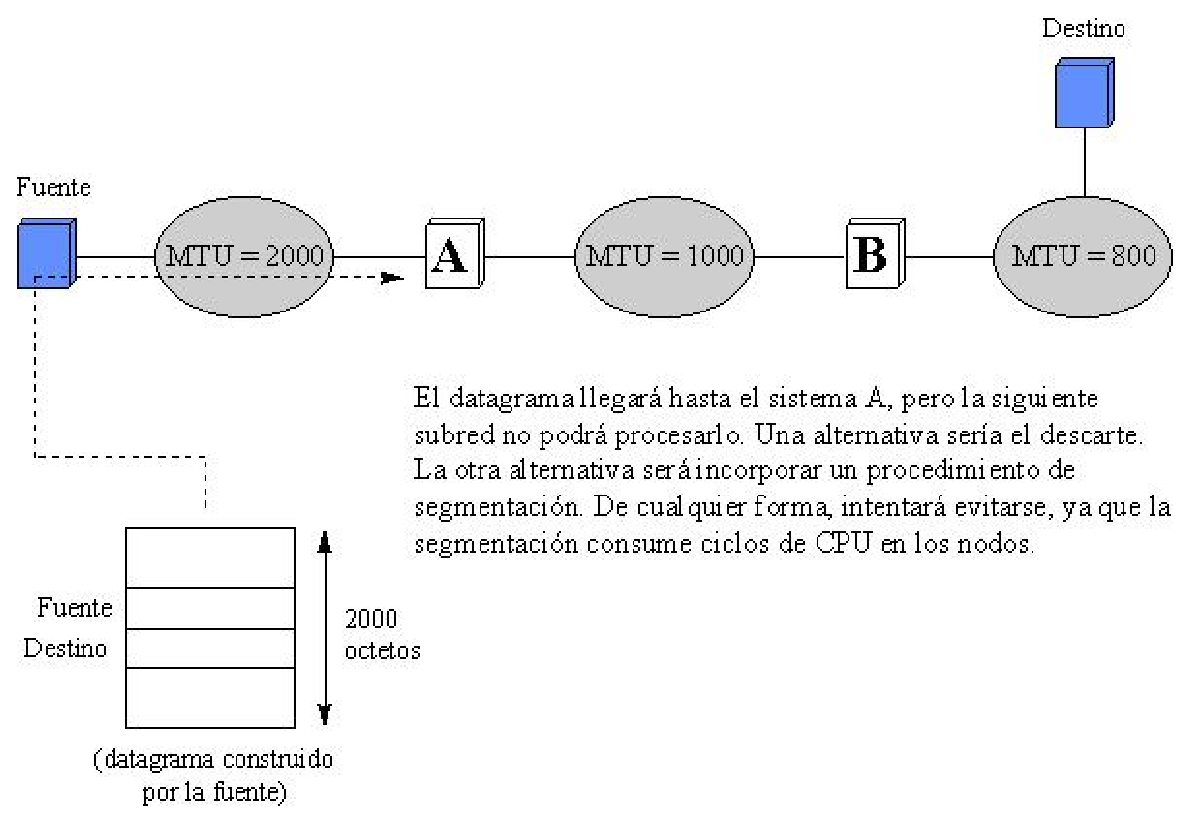
\includegraphics[width=\textwidth, height=8cm] {mtu.eps}
\caption{Rendimiento del protocolo IP}
\label{fig:mtu_ip}
\end{figure}

Estos son los puntos cr�ticos que afectan el rendimiento de una red \emph{IP}, no se conocen mecanismos de control. El dise�o de un protocolo es una lucha constante contra entre ganancias y p�rdidas de eficiencia.

\subsection{Protocolo de Control de Transferencia. TCP}

Proporciona un mecanismo fiable para la transferencia de flujos de informaci�n. Aunque est� �ntimamente relacionado con IP, TCP es un protocolo independiente de prop�sito general. Al ser un protocolo de alto nivel (4 en OSI) su funci�n es que grandes vol�menes de informaci�n lleguen a su destino correctamente, pudiendo recobrar la p�rdida espor�dica de paquetes. El protocolo TCP tiene las siguientes caracter�sticas:

\begin{itemize}
	\item Proporciona comunicaci�n bidireccional completa mediante circuitos virtuales. 
	\item Desde el punto de vista del usuario la informaci�n es transmitida por flujos de datos. 
	\item Confiabilidad en la transmisi�n de datos por medio de:
	\begin{itemize}
		\item Asignaci�n de n�meros de secuencia a la informaci�n segmentada. 
		\item Validaciones por suma (checksum). 
		\item Reconocimiento de paquetes recibidos. 
	\end{itemize}
\end{itemize}

\paragraph{Fiabilidad en la transferencia de TCP.}

Cada vez que un paquete es enviado se inicializa un contador de tiempo, al alcanzar el tiempo de expiraci�n, sin haber recibido el reconocimiento, el paquete se reenv�a. Al llegar el reconocimiento el tiempo de expiraci�n se cancela. \\

A cada paquete que es enviado se le asigna un n�mero de identificador, el equipo que lo recibe deber� enviar un reconocimiento de dicho paquete, lo que indicar� que fue recibido. Si despu�s de un tiempo dado el reconocimiento no ha sido recibido el paquete se volver� a enviar. Obs�rvese que puede darse el caso en el que el reconocimiento sea el que se pierda, en este caso se reenviar� un paquete repetido. \\

Utiliza el principio de ventana deslizable para esperar reconocimientos y reenviar informaci�n. Se define un tama�o de la ventana, que ser�an el n�mero de paquetes a enviar sin esperar reconocimiento de ellos. Conforme se recibe el reconocimiento de los primeros paquetes transmitidos la ventana avanza de posici�n enviando los paquetes siguientes. Los reconocimientos pueden recibirse en forma desordenada. \\

Si el protocolo s�lo contara con reconocimientos positivos, gran parte de la capacidad de la red estar�a desperdiciada, pues no se enviar�an m�s paquetes hasta recibir el reconocimiento del �ltimo paquete enviado. El concepto de ventana deslizante hace que exista una continua transmisi�n de informaci�n, mejorando el desempe�o de la red.

\subsection{Protocolo de Datagramas de Usuario. UDP}

Proporciona de mecanismos primordiales para que las aplicaciones se comuniquen entre si en m�quinas remotas. Provee un servicio no confiable orientado a no conexi�n, por lo que el programa tiene toda la responsabilidad del control de confiabilidad, mensajes duplicados o perdidos, retardos y paquetes fuera de orden. 

Este protocolo deja a la aplicaci�n la resposabilidad de una transmisi�n fiable. Con �l puede darse el caso de que los paquetes se pierdan o bien no sean reconstru�dos de forma adecuada. Permite un intercambio de datagramas m�s directo entre aplicaciones, por esta raz�n, es id�neo para software que busque optimizaci�n en el ancho de banda consumido, ya que, UDP no sobrecarga la red con confirmaciones y avisos de datagramas desordenados o perdidos. Puede y deber�a elegirse para aquellas que no demanden una gran cantidad de datagramas para operar �ptimamente, como es el caso de Voz sobre IP.

\subsection{Unicast {\it versus} Multicast}

Los servicios ``tradicionales'' de Internet est�n basados en lo que se conoce como IP Unicast, es decir, datagramas con un �nico origen y un �nico destino. En este caso, la comunicaci�n se denomina ``uno a uno''. Sin embargo, en situaciones en las que hay m�s de dos participantes en la comunicaci�n, la utilizaci�n de IP Unicast no es eficiente, puesto que hay que enviar la misma informaci�n a varios destinatarios simult�neamente, lo que puede sobrecargar a los emisores y la red. \\

\begin{figure}[hbt]
\centering
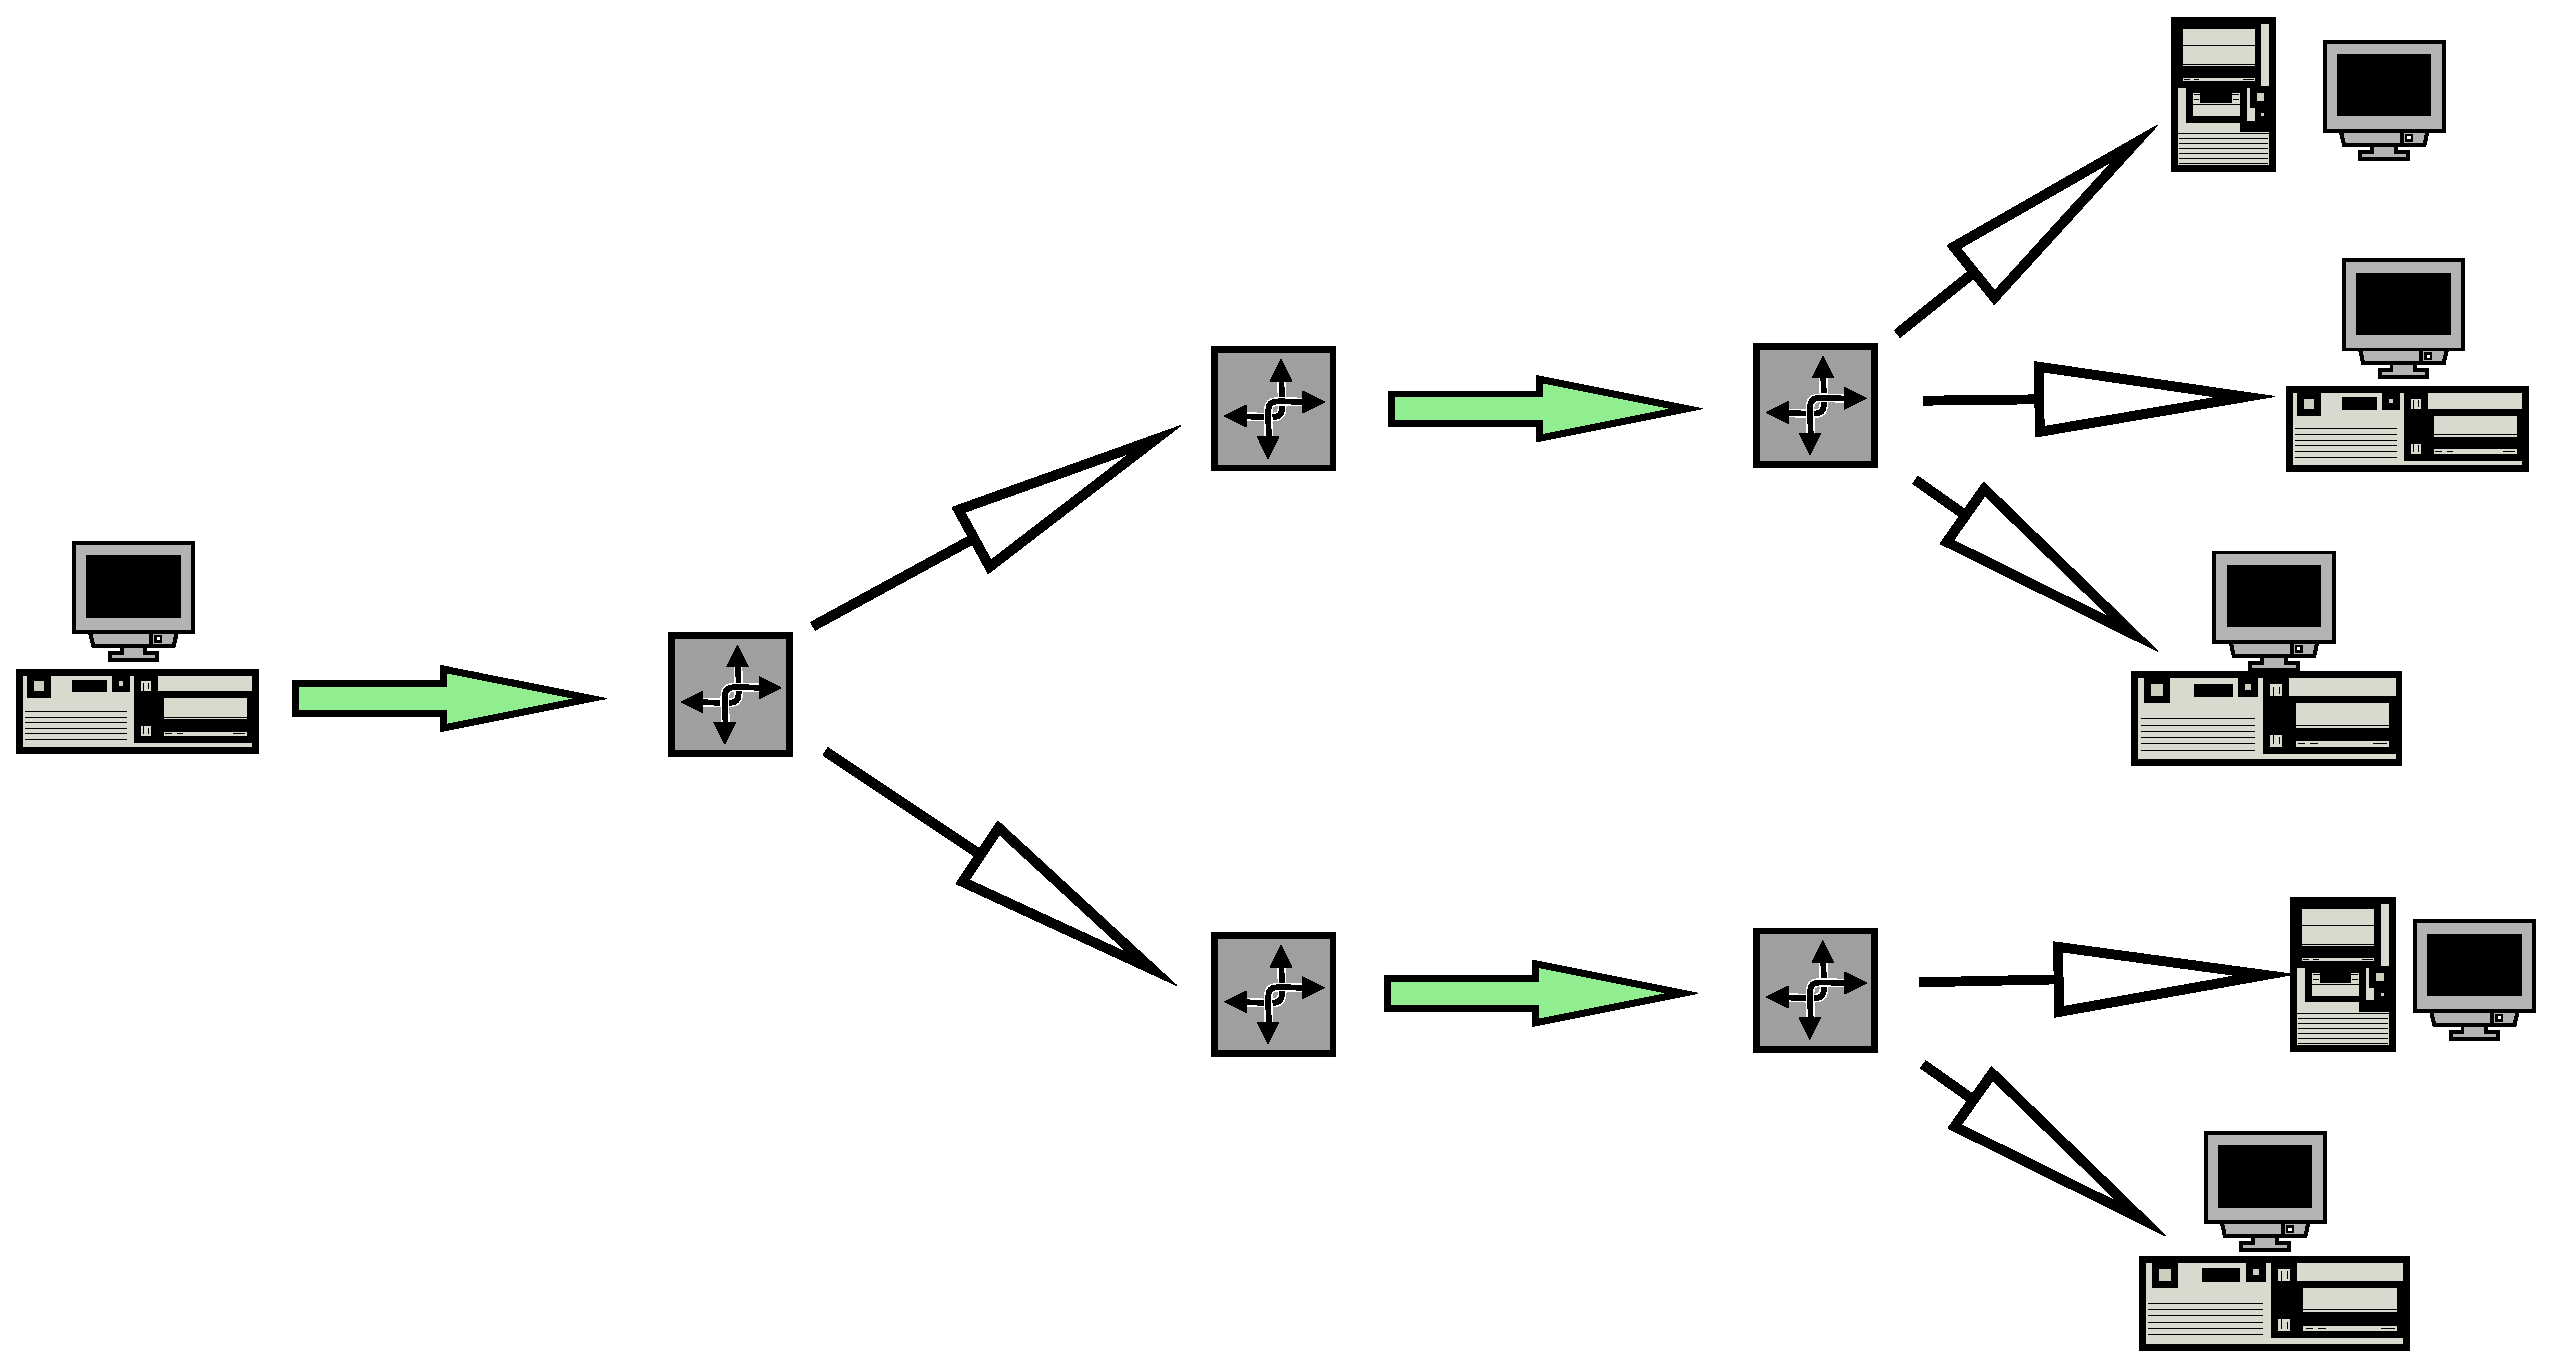
\includegraphics[width=10cm, height=5cm] {multicast.eps}
\caption{Funcionamiento de IP Multicast}
\label{fig:ip_multicast}
\end{figure}

Tradicionalmente, este problema ha sido resuelto mediante la utilizaci�n de ``reflectores'' (o Unidades de Control Multipunto , MCU, seg�n la terminolog�a \emph{H.323}), que son equipos a los que se conectan todos los participantes y que se encargan de la replicaci�n de todos los datagramas que env�a un participante al resto de ellos. Esta soluci�n plantea varios problemas, sobre todo referentes al consumo excesivo de ancho de banda en la red. Frente a esta soluci�n surge la alternativa IP Multicast, que consiste en que la red se encargue de hacer llegar los datagramas enviados por el emisor a un grupo de receptores. \\

La idea de grupo se implementa mediante un rango especial de direcciones IP y la suscripci�n o no a un determinado grupo es din�mica y la decide el receptor en funci�n de s� est� interesado o no en recibir los datagramas dirigidos a dicho grupo. Lo m�s importante es que la propia red se encarga de
replicar los paquetesparaque lleguen a todos los suscriptores del grupo. Adem�s, todo ello se realiza de modo que por cada enlace de la red solo circule un paquete (figura 1), duplic�n�dose �ste en aquellos momentos en los que se llegue a una bifurcaci�n en el camino hacia los destinatarios. \\

Cuando inicialmente se dise�o el esquema de direccionamiento en Internet se definieron varias clases de direccio�nes. La clase D se reserv� para las direcciones multidestino, esto es, el rango que va desde la direcci�n 224.0.0.0 a la 239.255.255.255. Dichas direcciones son conocidas como ``direcciones de grupo'' o multicast. De todo este rango, ciertas direcciones est�n reservadas para un uso espec�fico mientras que otras quedan libres para que las usen las aplicaciones que utilizan
los servicios IP Multicast.

\subsection{IPv6, la pr�xima generaci�n IP}

El protocolo IP en su versi�n 6 (IPv6, a partir de ahora), surge como un sucesor de la versi�n 4, que pronto se quedar� corta de espacio de direcciones, debido al crecimiento exponencial de Internet. \\

Al ver en el horizonte estos problemas, el IETF comenz� a trabajar en 1990 en una versi�n nueva de IP, que ser�a m�s eficiente y con un rango de direcciones virtualemente inagotable, siendo adem�s m�s flexible, eficiente y segura. Adem�s, de prestar una mayor atenci�n al tipo de servicio, para poder atender adecuadamente al tr�fico multimedia que se avecina. Los cambios de IPv6 respecto de IPv4 son, de forma resumida:
\begin{itemize}
	\item Expansi�n de las capacidades de direccionamiento. IPv6 incrementa el tama�o de las direcciones de 32 bits (IPv4) a 128 bits, para soportar m�s niveles en la jerarqu�a de direccionamiento, un n�mero mayor de nodos direccionables, y un sistema de autoconfiguraci�n de direcciones. 
	\item Simplificaci�n de la cabecera. Algunos campos de la cabecera del IPv4 son eliminados o pasan a ser opcionales, tanto para reducir el coste de procesamiento como el tama�o de la cabecera. 
	\item Mayor flexibilidad para extensiones y nuevas opciones. En IPv6 no existe un campo opciones, como tal. Eliminando as� las limitaciones de tama�o en la cabecera, e introduciendo una gran flexibilidad en el desarrollo de nuevas opciones. 
	\item Capacidades de control de flujo. Se a�aden capacidades que permiten marcar los paquetes que pertenezcan a un determinado tipo de tr�fico, para el cual el remitente demanda una calidad mayor a la especificada por defecto o servicios en tiempo real. 
	\item Capacidades de autenticaci�n y privacidad de datos. IPv6 provee extensiones para soportar autenticaci�n, e integridad y confidencialidad de datos.
\end{itemize}

\subsubsection{Direcciones IPv6}

Con un octeto se pueden representar los n�meros de 0 a 255. Por tanto las direcciones IPv4 se componen de cuatro octetos, o 32 bits, lo cual genera m�s de cuatro millones de direcciones. En IPv6 las direcciones se componen de 16 octetos, es decir 128 bits. Esto dar�a lugar a 2 128 direcciones, m�s o menos 340 sextillones. No obstante, esta cifra no se alcanza, ya que parte de los d�gitos identifican el tipo de direcci�n, con lo que se quedan en 3800 millones. En cualquier caso se garantiza que no se acabar�n en un plazo razonable. \\

Hay tres tipos de direcciones: \emph{unicast}, \emph{anycast} y \emph{multicast}. Las direcciones \emph{unicast} identifican un s�lo destino. Un paquete que se env�a a una direcci�n unicast llega s�lo al ordenador al que corresponda. En el caso de las direcciones \emph{anycast} se trata de un conjunto de ordenadores o dispositivos, que pueden pertenecer a nodos diferentes. Si se env�a un paquete a una de estas direcciones lo recibir� el ordenador m�s cercano de entre las rutas posibles. Las direcciones \emph{multicast} definen un conjunto de direcciones pertenecientes tambi�n a nodos diferentes, pero ahora los paquetes llegan a todas las m�quinas identificadas por esa direcci�n. \\

\subsubsection{Conversi�n formato IPv4 $\leftrightarrows$ IPv6}

�sta es una direcci�n de 32 bits: $192.9.32.12$ y �sta es una direcci�n de 128 bits: $BAF7:7432:FFFF:FFFF:7433:73F9:FFAA$. Puede observarse que las direcciones IPv4 se forman con cuatro n�meros decimales, que como ya se ha dicho van de 0 a 255. Para las direcciones IPv6 se usan n�meros hexadecimales. Para representar una direcci�n IPv4 con IPv6 se ponen a cero los cuartetos a partir del bit 33: $0000:0000:0000:0000:0000:C009:200C$ Esta notaci�n puede ser simplificada como $::192.9.32.12$ para equipos que no entienden IPv6 y como $::FFFF:192.9.32.12$ para equipos que s� entienden IPv4.

\subsection{RFC's de IP}

M�s informaci�n sobre el Protocolo Internet se encuentra en estos RFC's:

\begin{description}
	\item {RFC 791} Definici�n t�cnica del protocolo IP. 
	\item {RFC 1122} Especificaci�n de actualizaciones y correciones efectuadas.
	\item {RFC 1812} Requisitos y est�ndares que deben cumplir los fabricantes de encaminadores.
	\item {RFC 1108} Opciones de seguridad.
\end{description}

\section{RTP/RTCP}

RTP es un acr�nimo de Real Time Protocol y como su nombre indica, es un protocolo dise�ado para la transmisi�n de datos en tiempo real. Existen otros protocolos de tiempo real, pero �ste el m�s usado y est� estandarizado. En este proyecto se ha utilizado el protocolo \emph{RTP} para la transmisi�n de audio, ya que es un contenido con caracter�sticas intr�nsecas de tiempo real. En esta seccion, hay una peque�a introducci�n a este protocolo, as� como su aplicaci�n al audio.

\subsection{Introducci�n}

\emph{RTP} (\emph{Real Time Protocol}) provee servicios de transmisi�n de datos con caracter�sticas de tiempo real, como sonido y v�deo interactivos. Estos servicios incluyen identificaci�n del tipo de contenido (\emph{payload}), n�meros de secuencia, marcas de tiempo y monitorizaci�n de p�rdidas. \\

Normalmente, las aplicaciones suelen emplear \emph{RTP} sobre \emph{UDP} para poder utilizar sus capacidades de multiplexaci�n y servicios de comprobaci�n de errores; ambos protocolos contribuyen a la funcionalidad del protocolo de transporte.
Otras razones de peso para usar UDP en vez de TCP, es que RTP se ha dise�ado pensando en los servicios multicast, para lo cual la conexion TCP no es apropiada por problemas de escalabilidad. En segundo lugar, RTP se ha dise�ado para datos en tiempo real, la fiabilidad del transporte no es tan importanate como la recepci�n en el tiempo adecuado. TCP implementa la fiabilidad de transmisi�n usando retransmisi�n de paquetes, lo cual puede ser un incoveniente, ya que si se congestiona la red, la calidad ser�a muy inferior y congestionar�a aun mas la red intentando retransmitir paquetes perdidos.
 Sin embargo, \emph{RTP} se puede utilizar con cualquier otra red o protocolo de transporte subyacente. \emph{RTP} soporta transmisi�n de datos a m�ltiples destinos utilizando distribuci�n por multicast si lo proporciona la red subyacente. \\

Este protocolo no proporciona por si mismo ning�n mecanismo para asegurar que los datos llegan en el momento que deber�an o cualquier otra garant�a de calidad de servicio, deja esta tarea a las capas de aplicaci�n. No garantiza que los datos llegan ni tampoco que llegan en orden, tampoco asume que la red subyacente se encarga de que los paquetes lleguen en orden. Por estas razones RTP, se implementa generalmente dentro de la aplicaci�n, pues estos sistemas de recuperaci�n de paquetes perdidos o de control, deben ser implementados a nivel de aplicaci�n. \\

RTP incorpora marcas de tiempo espec�ficas para cada medio transportado (timestamp), que se utilizan para eliminar jitter (intraflujo) y para sincronizar entre flujos (interflujo). Varios paquetes pueden llevar la misma marca de tiempo si pertenecen a la misma unidad de datos a nivel de aplicaci�n, por ejemplo el mismo cuadro de v�deo. Incorpora n�meros de secuencia para que el receptor sea capaz de reconstruir la secuencia emitida, pero los n�meros de secuencia tambi�n se pueden utilizar para determinar la posici�n de un paquete sin necesidad de reproducirlos en orden. El \emph{payload} o identificador de carga, especifica el formato de datos, as� como el esquema de compresi�n y descompresi�n, con este identificador, la aplicaci�n receptora sabe como interpretar y reproducir los datos. Los distintos payload se definen en el RFC 1890. Otra funci�n de RTP es identificar la fuente de los datos, lo que le permite a la aplicaci�n receptora conocer de donde vienen los datos, por ejemplo en este proyecto permite identificar qui�n est� hablando. \\

\emph{RTP} representa un nuevo estilo de protocolos siguiendo los principios de enmarcado a nivel de aplicaci�n y procesamiento de capas propuesto por Clark y Tennenhouse \cite{Tennenhouse}. Esto es, \emph{RTP} est� pensado para ser maleable y as� proporcionar la informaci�n necesaria por una aplicaci�n particular y a menudo estar� integrado en el procesamiento de la aplicaci�n en lugar de estar implementado en una capa independiente. \emph{RTP} es un marco de protocolos que intencionadamente no est� completo. Al contrario que los protocolos convencionales, en los cuales las funciones adicionales pueden aparecer haciendo el protocolo m�s general o a�adiendo mecanismo de opciones que requerir�a un \emph{parser}, \emph{RTP} est� pensado para ser adaptado a trav�s de modificaciones y/o adiciones a las cabeceras como sea necesario. Existen otras aplicaciones a las que se puede aplicar \emph{RTP} como el almacenamiento de datos continuos, simulaci�n interactiva distribuida, control activo de divisas, y aplicaciones de control y medida. \\

\emph{RTP} consta de dos partes enlazadas muy de cerca:
\begin{description}
    \item [El protocolo de transporte de tiempo real (\emph{RTP})], para transportar los datos que tienen propiedades de tiempo real. Sus caracter�sticas se han comentado anteriormente.
    \item [El protocolo de control de \emph{RTP} (\emph{RTCP}).] Es el encargado de monitorizar la calidad del servicio y transportar la informaci�n sobre los participantes en una sesi�n. 
\end{description}

\paragraph{RTCP}

Real Time Control Protocol, es un protocolo dise�ado para trabajar conjuntamente con RTP. En una sesi�n RTP, los participantes se envian peri�dicamente distintos tipos de paquetes RTCP para tener informaci�n sobre la calidad de recepci�n y estad�sticas de paquetes RTP perdidos, informaci�n del numero de participantes (en multicast), informaci�n adicional de los participantes, entrar y abandonar sesiones, etc. A trav�s de RTCP se consigue:

\begin{description}
	\item[Monitorizaci�n de la calidad de servicio (QoS) y congesti�n de red.] Constituye la funci�n primaria de RTCP. Esta informaci�n es util a los emisores, a los receptores y a otras terceras partes interesadas (Gateways, etc.). El emisor puede ajustar su transmisi�n bas�ndose en esos informes, evaluando el rendimiento de la red para distribuciones multicast.
	\item[Identificaci�n de fuentes.] Las fuentes de datos se identifican en los paquetes RTP con identificadores de 32 bits generados aleatoriamente. Estos identificadores no aportan ningun tipo de informaci�n para el usuario final. Los paquetes RTCP SDES (Source Description, descripcion de fuente) contienen informaci�n textual: nombre del participante, telefono, direccion de correo electronico, localizaci�n, etc.
	\item[Sincroniacion Intermedia.] RTCP permite sincronizar fuentes de datos que procedan de distintas sesiones RTP, para ello emplea las marcas temporales de los paquetes RTP.
	\item[Escalado de la informaci�n de control.] Los paquetes RTCP se envian periodicamente entre los participantes, si el numero de participantes es grande, es necesario un compromiso entre la informaci�n actualizada y la sobrecarga de red. RTCP debe limitar el tr�fico de control en la red acorde a la sobrecarga.
\end{description}

El protocolo \emph{RTP}, no tiene porque ir acompa�ado de RTCP, ya que su unica mision es transportar los datos. De hecho, muchas aplicaciones de VoIP ni siquiera soportan RTCP, ya que no es vital para la comunicaci�n. Esta funcionalidad podr�a ser asumida parcial o totalmente por un protocolo de control de sesi�n separado.


\section{Negociaci�n de la sesi�n}

Hasta el momento, en apartados anteriores, se ha visto una serie de protocolos que se usan para transmitir los datos en tiempo real, pero para transmitir esos datos, antes es necesario negociar el inicio de la sesi�n que se quiere establecer. Esto es, definir o negociar una serie de par�metos, como pueden ser: los puertos de envio y recepcion de RTP, los codecs de audio empleados (payload), numero de participantes (redes multicast) etc. \\

Actualmente existen dos protocolos que se disputan este campo: H.323 y SIP. H.323 fue el primero en ser estandarizado por la ITU-T y usa una aproximaci�n m�s tradicional, basada en el protocolo Q.931 de la RDSI y en los est�ndares H.XXX anteriores. H.323 no se puede considerar un protocolo abierto (el estandar no est� liberado), pero ha sido la referencia de la industria hasta el momento. SIP, creado y estandarizado por IETF, -con apenas a�o y medio de existencia, y que todav�a se encuentra en estado de desarrollo y revisi�n; la primera versi�n del RFC 2543 apareci� en la primavera del 2001- se basa en un enfoque m�s ligero, del estilo de los protocolos de Internet, similar a HTTP (de hecho rehusa gran parte de los campos de cabecera, reglas de codificaci�n, c�digos de error y mecanismos de autenticaci�n).

\subsection{SIP {\it versus} H.323}

En esta parte se compara SIP y H.323. Ambos protocolos pueden usar y usan generalmente RTP para intercambiar los datos, por tanto la elecci�n de uno u otro no afecta a la calidad de servicio. Para realizar la comparaci�n entre H.323 y SIP se analizaran cuatro campos: complejidad, extensibilidad, escalabilidad y disponibilidad de servicios.

\begin{description}
	\item[Complejidad.] H.323 es el m�s complejo de los dos protocolos, su RFC suma alrededor de 700 p�ginas. En cambio, SIP, con las extensiones de control de llamadas y protocolos de descripci�n de sesi�n, tiene un RFC de 260 p�ginas. H.323 define cientos de elementos, mientras SIP tiene s�lo 37 cabeceras, cada una con un peque�o n�mero de valores y par�metros. H.323 usa una representaci�n binaria para sus mensajes, basados en ASN.1 y las reglas de codificaci�n de paquetes. SIP codifica sus mensajes como texto, similar a http y rtsp. Otra ventaja de SIP es que usa una solicitud simple que contiene toda la informaci�n necesaria, mientras muchos de los servicios H.323 requieren interacci�n entre los diferentes componentes del protocolo que son incluidos en el est�ndar.
	\item[Extensibilidad.] Es una prueba para medir un protocolo de se�alizaci�n de VoIP. Como con alg�n servicio usado excesivamente, las caracter�sticas de �ste proveen evoluci�n en el tiempo y como nuevas aplicaciones son desarrolladas. Esto hace compatibles las diferentes versiones. SIP se ha desarrollado teniendo en cuenta las lecciones de HTTP y SMTP (Simple Mail Transfer Protocol), ambas evolucionan con el tiempo y constituyen un rico conjunto de extensibilidad y compatibilidad de funciones.
H.323 tambi�n define mecanismos de extensibilidad, pero de forma m�s compleja.
	\item[Escalabilidad.] La escalabilidad es importante en el uso de Internet, ya que sus servicios tienden a crecer. En este caso, los protocolos deben ser comparados en diferentes niveles: 
	\begin{itemize}
		\item \emph{N�meros largos de dominios:} como H.323 fue creado originalmente pensado para usarse en una simple LAN, tiene algunos problemas con la escalabilidad, ni siquiera la versi�n m�s reciente define el concepto de zonas y procedimientos para usar la localizaci�n de usuarios. SIP, sin embargo, usa un m�todo de detecci�n de bucles verificando la historia del mensaje. 
		\item \emph{Tama�o de conferencias:} H.323 tiene soporte para multiconferencias con distribuci�n de datos (multicast), esto requiere un punto central de control, llamado Multipoint Controller (MC), para procesar y se�alizar, lo cual, tiende a convertirse en un embotellamiento para conferencias grandes. SIP no tiene necesidad de un MC central y la coordinaci�n de conferencia es completamente distribuida, mejorando la escalabilidad y complejidad, pero, ofrece un proveedor de servicios con menos control. 
	\end{itemize}
	\item[Servicios.] De un modo general SIP y H.323 proveen los mismos servicios, de igual manera nuevos servicios pueden ser incorporados. En conclusi�n, para servicios de control de llamadas, ambos SIP y H.323 proveen capacidades de servicios de intercambio. 
\end{description}

En extensibilidad SIP proporciona mayores recursos para nuevas implementaciones y compatibilidad con nuevas versiones. H.323 soporta menos mecanismos debido al uso de ASN.1 que restringe los campos sujetos a nuevas implementaciones. Existen numerosas propuestas para ampliar el protocolo SIP que todav�a no han sido publicadas como RFCs ni se han a�adido a SIP. Ejemplos son: el soporte para las primitivas MESSAGE, REFER � INFO, el modo de operaci�n requerido para atravesar NATs � las funcionalidades a�adidas de control de llamada. En escalabilidad SIP es totalmente distribuido con lo cual puede soportar conferencias de muchos participantes. En cambio H.323 presenta un esquema centralizado que reduce escalabilidad aunque tiene mayor control. 

\subsection{SDP}

El Protocolo de Descripci�n de Sesi�n (SDP) se usa para describir una sesi�n de multimedios dentro de una solicitud SIP, es decir, se usa para prop�sitos de inicio de sesi�n, invitaci�n a sesi�n, etc. El prop�sito de este protocolo es llevar informaci�n sobre el flujo de medios en sesiones multimedia que permiten a las personas recibir una descripci�n de la sesi�n para participar en ella. SDP es puramente un formato para la descripci�n de la sesi�n. No incorpora un protocolo de transporte, y esta pensado para usar diferentes protocolos de transporte apropiados: SIP, RTP, correo electr�nico (SMTP) que usa extensiones MIME, HTTP, etc. 
Este protocolo es un producto del Control de Sesi�n Multipartita de Multimedios (MMUSIC) grupo de trabajo de la IETF, RFC 2327. \\

En general, SDP debe llevar informaci�n suficiente para habilitar la uni�n de una sesi�n (con la posible excepci�n de claves de encriptaci�n) y anunciar los recursos a ser usados por no-participantes que pueden necesitarlos. Una descripci�n SDP incluye la siguiente informaci�n: 

\begin{itemize}
	\item Nombre de la sesi�n y prop�sito.  
	\item Tiempo en que la sesi�n est� activa.  
	\item Los medios que comprenden la sesi�n.   
	\item Informaci�n en c�mo recibir esos medios tal como direcciones, puertos y formatos.  
	\item La informaci�n adicional como el ancho de banda a ser usado en la conferencia y contactar informaci�n para la persona responsable de la sesi�n establecida. 
\end{itemize}

\begin{figure}[htb]
\centering
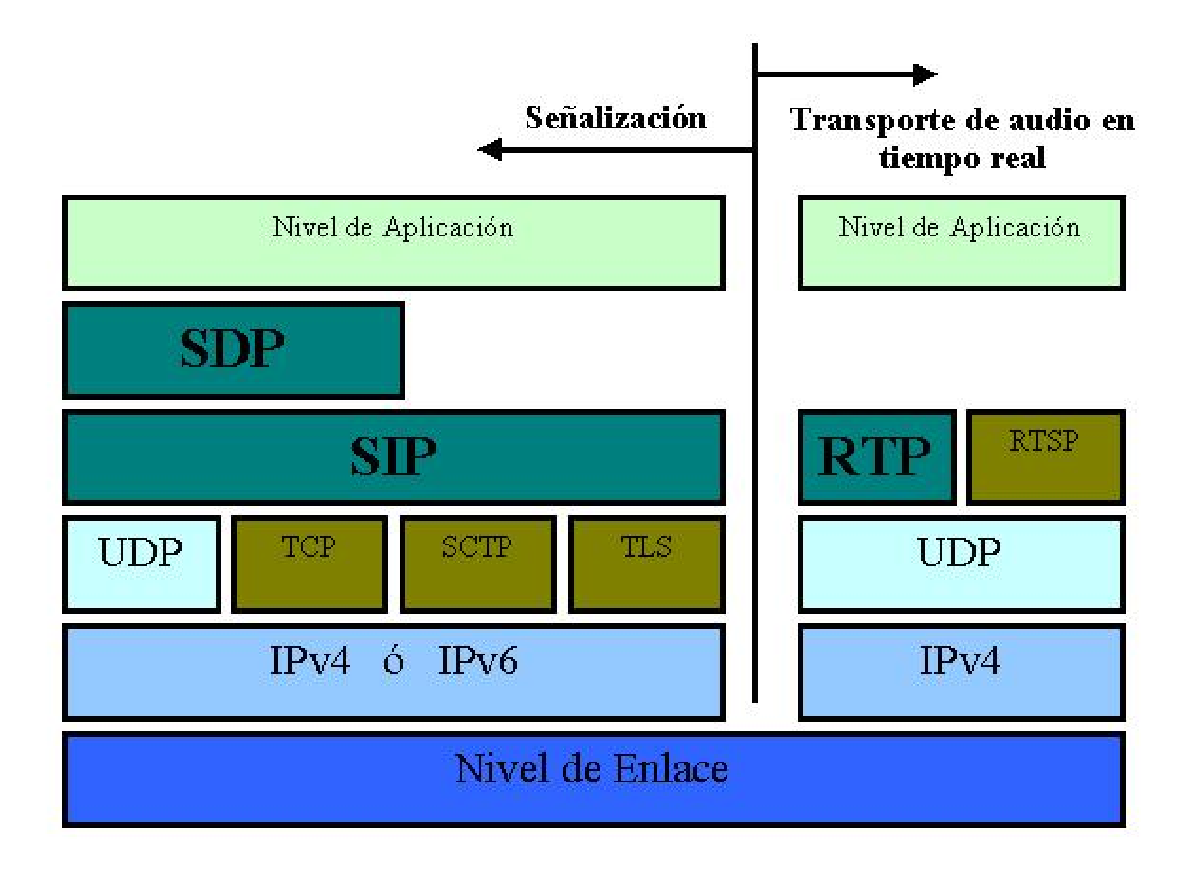
\includegraphics[width=8cm, height=5cm] {protocolos.eps}
\caption{Pila de protocolos}
\label{fig:protocolos}
\end{figure}

\section{XML}

XML, es el est�ndar de {\it Extensible Markup Language}. XML no es m�s que un conjunto de reglas para definir etiquetas sem�nticas que organizan un documento en diferentes partes, es decir, XML es un metalenguaje que define la sintaxis utilizada para definir otros lenguajes de etiquetas estructurados. \\

XML fue creado al amparo del {\it Word Wide Web Consortium} (W3C), organismo que vela por el desarrollo web partiendo de las amplias especificaciones de \emph{SGML}. Su desarrollo comenz� en 1996 y la primera versi�n sali� a la luz en febrero de 1998 bajo la definici�n de: ``Sistema para definir validar y compartir formatos de documentos en la web''. 

\paragraph{XML tiene como objetivos:}

\begin{itemize}
	\item XML debe ser directamente utilizable sobre Internet.
    \item XML debe soportar una amplia variedad de aplicaciones.
    \item XML debe ser compatible con \emph{SGML}.
    \item Debe ser f�cil la escritura de programas que procesen documentos XML.
    \item El n�mero de caracter�sticas opcionales en XML debe ser absolutamente m�nima, idealmente cero.
    \item Los documentos XML deben ser legibles por humanos y razonablemente claros.
    \item El dise�o de XML debe ser preparado r�pidamente.
    \item El dise�o de XML debe ser formal y conciso.
    \item Los documentos XML deben ser f�cilmente creables.
    \item La concisi�n en las marcas XML es de m�nima importancia.
\end{itemize}

\paragraph{Principales caracter�sticas}

\begin{itemize}
    \item Es una arquitectura abierta y extensible. No necesita versiones para que puedan funcionar en futuros aplicaciones. Los identificadores pueden crearse de manera simple y ser adaptados en el acto por medio de un validador de documentos (parser).
    \item Mayor consistencia, homogeneidad y amplitud de los identificadores descriptivos del documento con XML 
    \item Integraci�n de los datos de las fuentes m�s dispares. Se podr� hacer el intercambio de documentos entre las aplicaciones tanto en el propio PC como en una red.
 	\item Datos compuestos de m�ltiples aplicaciones. La extensibilidad y flexibilidad de este lenguaje permite agrupar una variedad amplia de aplicaciones, desde p�ginas web hasta bases de datos.
    \item Exportabilidad a otros formatos de publicaci�n (papel, web, etc.). El documento maestro de la edici�n electr�nica podr�a ser un documento XML que se integrar�a en el formato deseado de manera directa.
\end{itemize}

\paragraph{Estructura de XML}

XML consta de varias especificaciones (el propio XML sienta las bases sint�cticas y el alcance de su implementaci�n), pero las m�s importantes son dos:

\begin{description}
	\item [\emph{DTD} (Document Type Definition):] Definici�n del tipo de documento. Es, en general, un archivo/s que encierra una definici�n formal de un tipo de documento y, a la vez, especifica la estructura l�gica del  documento. Define tanto los elementos de un documento como sus atributos. El DTD del XML es opcional. En tareas sencillas no es necesario construir un DTD, entonces se tratar�a de un documento ``bien formado'' (well-formed) y si lleva DTD ser� un documento ``validado'' (valid).
	\item [\emph{XSL} (eXtensible Stylesheet Language):] Define o implementa el lenguaje de estilo de los documentos escritos para XML. Este est�ndar est� basado en el lenguaje de sem�ntica y especificaci�n de estilo de documento (\emph{DSSSL}, Document Style Semantics and Specification Language, ISO/IEC 10179).
\end{description}

\subsection{Est�ndares XML}

Los est�ndares Unicode e ISO/IEC 10646 para caracteres, RFC 1766 para identificaci�n de lenguajes, ISO 639 para c�digos de nombres de lenguajes, e ISO 3166 para c�digos de nombres de pa�ses, proporciona toda la informaci�n necesaria para entender la versi�n 1.0 de XML y construir programas que los procesen.

\section{Data Encryption Standard. DES}

DES es un esquema de cifrado sim�trico desarrollado en 1977 por el Departamento de Comercio y la Oficina Nacional de Est�ndares de EEUU en colaboraci�n con la empresa IBM, que se cre� con objeto de proporcionar al p�blico en general un algoritmo de cifrado normalizado para redes de ordenadores. Estaba basado en la aplicaci�n de todas las teor�as criptogr�ficas existentes hasta el momento, y fu� sometido a las leyes de USA. \\

Se basa en un sistema monoalfab�tico, con un algoritmo de cifrado consistente en la aplicaci�n sucesiva de varias permutaciones y sustituciones. Inicialmente los datos a cifrar se someten a una permutaci�n, con bloque de entrada de 64 bits (o m�ltiplo de 64), para posteriormente ser sometido a la acci�n de dos funciones principales, una funci�n de permutaci�n con entrada de 8 bits y otra de sustituci�n con entrada de 5 bits, en un proceso que consta de 16 etapas de cifrado. \\

En general, DES utiliza una clave sim�trica de 64 bits, de los cuales 56 son usados para el cifrado, mientras que los 8 restantes son de paridad, y se usan para la detecci�n de errores en el proceso. Como la clave efectiva es de 56 bits, son posible un total de 2 elevado a 56 = 72.057.594.037.927.936 claves posibles, es decir, unos 72.000 billones de claves, por lo que la ruptura del sistema por fuerza bruta o diccionario es s�mamente improbable, aunque no imposible si se dispone de suerte y una gr�n potencia de c�lculo. \\

Los principales inconvenientes que presenta DES son:
\begin{itemize}
    \item Se considera un secreto nacional de EEUU, por lo que est� protegido por leyes espec�ficas, y no se puede comercializar ni en hardware ni en sofware fuera de ese pa�s sin permiso espec�fico del Departamento de Estado.
    \item La clave es relativamente corta, tanto que no asegura una fortaleza adecuada. Hasta ahora hab�a resultado suficiente, y nunca hab�a sido roto el sistema. Pero con la potencia de c�lculo actual y venidera de los computadores y con el trabajo en equipo por Internet se cr�e que se puede violar el algoritmo, como ya ha ocurrido una vez, aunque eso s�, en un plazo de tiempo que no result� peligroso para la informaci�n cifrada.
    \item No permite longitud de clave variable, con lo que sus posibilidades de configuraci�n son muy limitadas, adem�s de permitirse con ello la creaci�n de limitaciones legales.
    \item La seguridad del sistema se ve reducida considerablemente si se conoce un n�mero suficiente textos elegidos, ya que existe un sistema matem�tico, llamado \emph{Criptoan�lisis Diferencial}, que puede en ese caso romper el sistema en 2 elevado a 47 iteraciones.
\end{itemize}

Entre sus ventajas cabe citar:

\begin{itemize}
    \item Es el sistema m�s extendido del mundo, el que m�s m�quinas usan, el m�s barato y el m�s probado.
    \item Es muy r�pido de calcular y f�cil de implementar.
    \item Desde su aparici�n nunca ha sido roto con un sistema pr�ctico.
\end{itemize}



\capitulo{An�lisis de requisitos}
\label{chp:analisisrequisitos}
%\newpage
%\thispagestyle{empty}
\minitoc
\newpage

Este es un proyecto fin de carrera y el proceso de desarrollo seguido es evolutivo, es decir,
a lo largo del tiempo, el software propuesto ha ido evolucionando a�adiendo y ampliando caracter�sticas, hasta llegar a la situaci�n actual. Por esta raz�n, en este cap�tulo se van a detallar todos los requisitos funcionales de la versi�n 0.10 de \software , sin detallar el proceso de evoluci�n realmente seguido. \\

El ciclo de dise�o es semejante a una espiral (Figura \ref{fig:diseno}). La elecci�n de este tipo de dise�o se debe a que: se adapta bien a la metodolog�a procedimental, s�lo hay un �nico desarrollador, hay unos objetivos m�nimos a cumplir y es relativamente f�cil ampliar car�cter�sticas, evaluando la viabilidad de cada una.

\begin{figure}[htb]
\centering
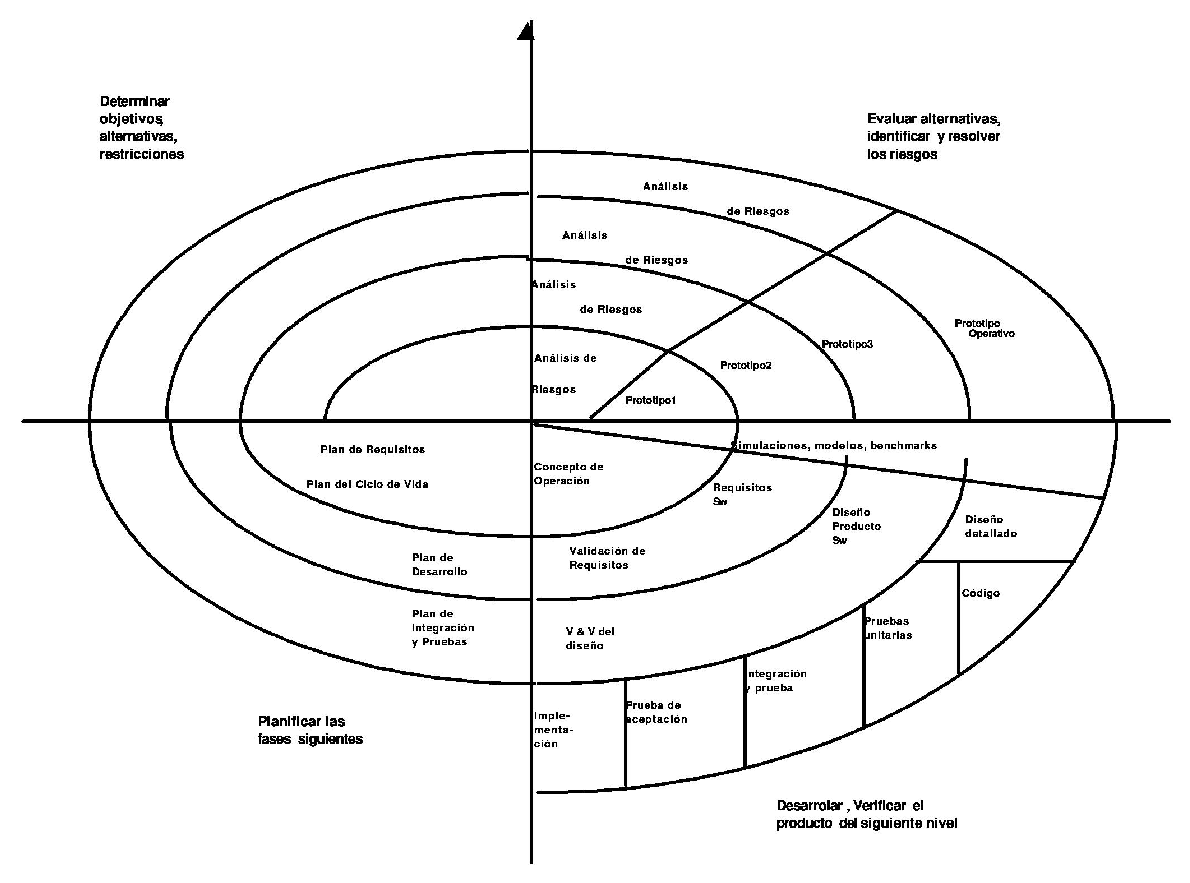
\includegraphics[width=\textwidth, height=12cm] {diseno.eps}
\caption{Proceso de dise�o del sotware.}
\label{fig:diseno}
\end{figure}

\section{Consideraciones previas}

El proyecto consta de dos programas complementarios, pero independientes. El programa principal se llama \software \  y es el software propuesto inicialmente en el proyecto. Es el encargado de transmitir el audio por canales RTP al programa remoto de otro usuario. El \textbf{Proxy SSIP} es la otra parte del proyecto -una ampliaci�n- y principalmente realiza la funci�n de la negociaci�n de inicio de sesi�n, pero, no es necesaria su instalaci�n, ya que fue desarrollado para casos espec�ficos comentados m�s adelante. Los requisitos de ambos programas se analizar�n por separado. La ilustraci�n \ref{fig:diagrama_proxy} muestra el uso del proxy. 

\begin{figure}[htb]
\centering
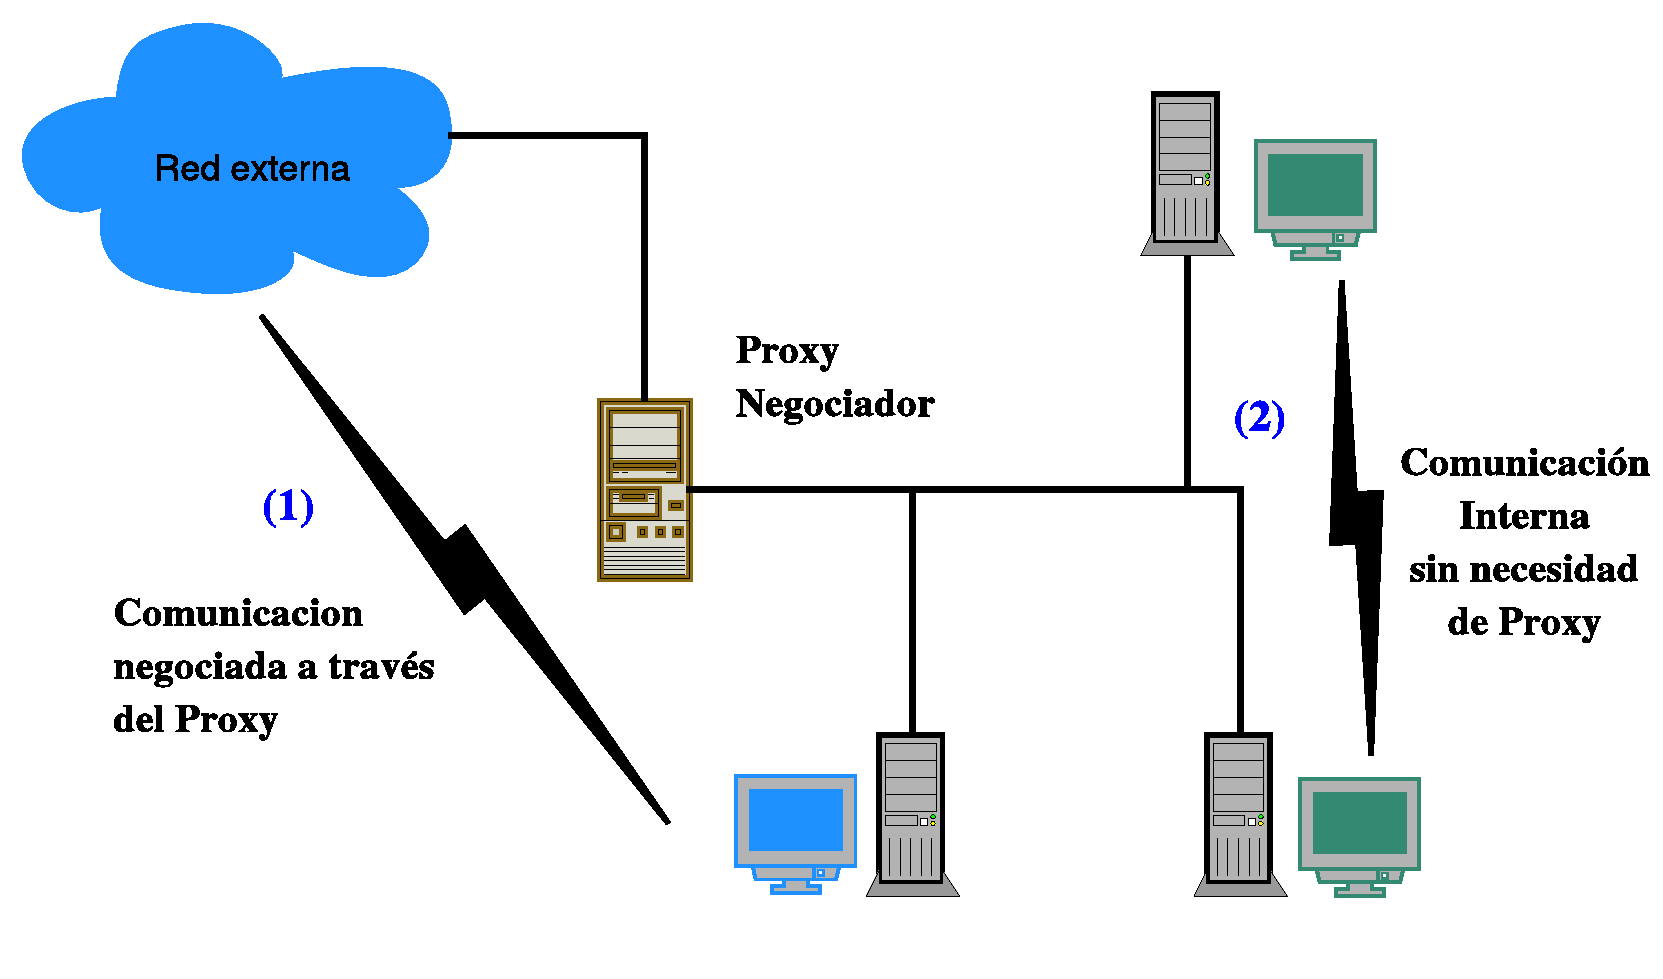
\includegraphics[width=\textwidth] {diagrama_proxy.eps}
\caption[Ejemplo de funcionamiento]{Ejemplo de uso del software.}
\label{fig:diagrama_proxy}
\end{figure}

En la situaci�n \textbf{(1)}, se ejemplifica el uso del proxy. El proxy instalado en la m�quina que hace de pasarela entre la red local y otra red (por ejemplo, Internet), ha gestionado la negociaci�n de sesi�n, mientras que en la situaci�n \textbf{(2)} el proxy no ha intervenido para nada. \\

Hay que se�alar que en el cap�tulo \ref{chp:plan_proyecto} ya se ha realizado un an�lisis de viabilidad, se han especificado los requisitos m�nimos propuestos para el proyecto y se ha explicado los motivos de la realizaci�n de este proyecto, entre otros. En este cap�tulo se va a detallar un completo an�lisis de requisitos de todo el sistema, pero partiendo del primer an�lisis ya realizado. Es obvio, que cualquier ampliaci�n a�adida al proyecto era viable, de otro modo no se llevar�a a cabo, por lo que, no se comentar�a en esta memoria.

\section{Visi�n general}

La complejidad filnal de todo el sistema es elevada, por lo que es necesario las especificaciones detalladas del mismo, lo que ofrecer� una gu�a para el dise�o. Los aspectos englobados son los siguientes:

\begin{itemize}
	\item Entorno de desarrollo.
	\item Entorno de operaci�n.
	\item Configuraci�n y operaci�n.
	\item Arquitectura funcional del sistema.
\end{itemize}

Los dos �ltimos aspectos son espec�ficos de cada programa (\software \  y \textbf{Proxy SSIP}), ser�n tratados dentro de sendas secciones posteriormente. Adem�s de estas especificaciones gen�ricas, se incluyen las especificaciones funcionales en las que se detallan los comportamientos y caracter�sticas de los diferentes m�dulos necesarios para la realizaci�n del proyecto.

\subsection{Entorno de desarrollo}

Para el desarrollo de este proyecto es necesario un entorno constituido por dos m�quinas PC conectadas a trav�s de una red de �rea local. Aunque para las etapas de an�lisis, dise�o y prueba, basta con una, s�lo es necesario el segundo PC para las pruebas de software. \\

Ambas m�quinas deber�n tener Linux instalado con un kernel 2.4 o superior, sistema gr�fico operativo (XFree86), una tarjeta de sonido compatible, soporte de dicha tarjeta en el kernel y unos altavoces -o auriculares- y un micr�fono para acceder a ella. Adem�s, deber� contar con el entorno de desarrollo apropiado para C, con su correspondiente compilador y depurador y una serie de librer�as que se detallar�n posteriormente. Por �ltimo, deber� disponer de toda la documentaci�n necesaria referente al manejo de hilos, acceso a drivers de audio mediante OSS, uso de las librer�as Glib y GTK+, los est�ndares de RTP/RTCP, etc. \\

A modo de resumen, el hardware, software y documentaci�n necesaria son:

\paragraph{Hardware:}
\begin{itemize}
	\item Dos PC's.
	\item Tarjeta de red y red \emph{IP} de �rea local.
	\item Tarjeta de sonido, altavoces y micr�fono.
	\item Acceso a Internet (para obtener documentaci�n).
\end{itemize}

\paragraph{Software:}
\begin{itemize}
	\item Sistema operativo GNU/Linux con kernel 2.4 o superior.
	\item Kernel configurado que soporte la tarjeta de sonido y la LAN.
	\item Compiladores y herramientas GNU para C: gcc, electric-fence, memprof y make.
	\item Librer�as Glib y GTK+ junto con sus cabeceras de C (``includes'').			
	\item Herramientas de mantenimiento: diff y patch.
	\item Analizador de red software: tcpdump y ethereal.
	\item Editor de c�digo fuente: FTE.
	\item Editor de interfaces gr�ficas de GTK+2.0: glade-2.
	\item Entorno de desarrollo integrado: KDevelop.
\end{itemize}

\paragraph{Documentaci�n:}
\begin{itemize}
	\item Est�ndares para SIP y RTP/RTCP. Informaci�n de H.323.
	\item Documentaci�n sobre el uso de GLib y GTK+
	\item Documentaci�n sobre el acceso a drivers OSS.
	\item P�ginas del manual de Linux.
\end{itemize}

\subsection{Entorno de operaci�n}

El entorno de operaci�n es el entorno en el que va a ser ejecutado el software, centr�ndose en lo necesario para desenvolver un funcionamiento normal. El software se puede encontrar en {\it http://asubio.sourceforge.net}, en forma de tarball comprimido. Una vez descargado, habr� que configurarlo, compilarlo e instalarlo, usando la herramienta {\it make}. Para que la compilaci�n finalice correctamente es necesario tener instaladas en el sistema estas librer�as: GLib y GTK+ (version $>=$ 2.0) y libxml-2. \\

Adem�s de todo esto, ser� imprescindible una tarjeta de sonido debidamente configurada y accesible. Para poder operar correctamente, es necesario una red IP, y si dentro de esa red hay un grupo de usuarios que pretenden mantener conversaciones con otros usuarios que no pertenecen a su red (�mbito), ser� necesario la instalaci�n del \textbf{Proxy SSIP} que se encargue de negociar las sesiones externas. 

\section{\software}

An�lisis del programa \software .

\subsection{Arquitectura funcional}

La arquitectura funcional del programa \software \  consta de las siguientes �reas funcionales:

\subsubsection{Interfaz Gr�fica Usuario. GUI}

Ser� la v�a de acceso de los usuarios al sistema. Se realizar� como una aplicaci�n de fondo, minimalista, por lo que debe ser peque�a y completa, debe dar la posibilidad de ejecutar diversas acciones. Cada una de estas acciones desembocar� en una sucesi�n de cajas de di�logo que ir�n preguntando al usuario por todos aquellos valores requeridos. \\

Deber� contener servicios de valor a�adido, como por ejemplo la posibilidad de usar una libreta de direcciones -agenda de contactos- para almacenar las direcciones de otros usuarios. Tambi�n ser�a interesante disponer de manejadores para el volumen del audio, etc.

\subsubsection{Acceso, tratamiento y transmisi�n de audio}

Es quiz�s la parte compleja de \software , porque representa el n�cleo que implementa todas las operaciones con el sonido y la negociaci�n de sesiones. Debe ser capaz de gestionar m�ltiples sesiones de forma simult�nea, mediante el uso de hilos de ejecuci�n paralelos. \\

Esta parte debe estar formada por varios subsistemas que permitan dividir el desarrollo y simplificarlo. Adem�s la aquitectura del software, ser� totalmente abierta, habr� tres tipos de ``plugins'' que permitir�n ampliar las funcionalidades:
\begin{description}
	\item [Plugins de compresi�n de sonido. \textbf{Codec\_Plugin}.] Tambi�n llamados ``codecs'' de audio � ``vocodecs''. Cada \emph{codec} implementar� un algoritmo de compresi�n-descompresi�n de audio, de esa forma, es muy f�cil incorporar nuevos compresores de audio sin modificar el programa.
	\item [Plugins de Entrada-Salida de audio. \textbf{InOut\_Plugin}.] Este tipo de plugin, ser� encargado de proveer las funiones de lectura y escritura de audio en el PC. Principalmente acceder�n a la tarjeta de sonido para capturar y reporducir el sonido. Tambi�n deben contener las funciones que controlen el volumen y ganancia de los altavoces y micr�fono.
	\item [Plugins de Effectos generales. \textbf{Effect\_Plugin}.] Permiten desarrollar plugins para aumentar las funcionalidades del sistema original, podr�n por ejemplo grabar conversaciones, modificar la voz del usuario, suprimir efectos de eco, etc.
\end{description}

Otras consideraciones a tener en cuenta son: 
\begin{itemize}
	\item Cada sesi�n RTP podr� tener plugins de codecs y de efectos diferentes a otras y adem�s configurados de distinto modo.
	\item La posibilidad de cifrar sesiones con alg�n algoritmo de cifrado. Se debe usar compilaci�n condicional para crear varias versiones del programa. As� se podr� exportar a pa�ses como USA, etc.
	\item Posicionaiento de los bytes. Linux ``corre'' en muchas arquitecturas diferentes. Existen arquitecturas con ordenamiento de bytes \emph{BIG\_ENDIAN}, los m�s significativos primero, como el PowerPC de Motorola (Apple) y otras con ordenamiento \emph{LITTLE\_ENDIAN}, los bytes menos significativos primero como ocurre en I386 de Intel. El programa deber� solucionar estos inconvenientes, para que la aplicaci�n sea tan portable como lo es Linux.
\end{itemize}

\subsubsection{Gesti�n de la Agenda de contactos}

El programa dispondr� de una agenda de contactos, para guardar a los usuarios. Ser� un fichero en formato XML, con el siguiente DTD:

\begin{center}
\begin{boxit}
\begin{verbatim}
<!DOCTYPE agenda [
<!ELEMENT contacto (nombre[1], usuario[1], 
			        host[1], puerto[1], 
		            descripcion[1], foto[1])
<!ELEMENT contacto (default*, ignore[1])>
<!ATTLIST contacto ignore (TRUE | FALSE) #REQUIRED>
<!ATTLIST contacto default (TRUE | FALSE) #IMPLIED>
<!ELEMENT nombre (#PCDATA)> 
<!ELEMENT usuario (#PCDATA)> 
<!ELEMENT host (#PCDATA)> 
<!ELEMENT puerto (#PCDATA)> 
<!ELEMENT descripcion (#PCDATA)> 
<!ELEMENT foto (#PCDATA)> 
]>
\end{verbatim}
\end{boxit}
\end{center}

El usuario podr� modificar todos estos campos desde una interfaz gr�fica, sin necesidad de editar manualmente el fichero XML. Tambi�n podr� a�adir nuevos usuarios, borrar uno existente, etc. Este fichero debe contener como m�nimo un contacto, el que representa a todos los usuarios que no est�n en la agenda. Ese contacto define el comportamiento -aceptar o rechazar autom�ticamente las llamadas y la foto- con los usuarios desconocidos (los que no est�n en la agenda) y nunca podr� ser borrado. \\

$<$ \textbf{contacto} $>$ representa un contacto de la agenda. Podr� tener dos atributos:
\begin{itemize}
	\item \textbf{default}: si aparece este atributo y tiene el valor de \emph{TRUE} significa que es el usuario por defecto. Siempre debe existir un usuario por defecto en el fichero para que se considere v�lido.
	\item \textbf{ignore}: si aparece este atributo y tiene el valor de \emph{TRUE} significa que todas las llamadas de ese usuario ser�n igonradas.
\end{itemize}

Y estar� compuesto obligatoriamente por los campos que se explican a continuaci�n:

\begin{itemize}
	\item \textbf{nombre}: nombre de pila del usuario.
	\item \textbf{usuario}: nombre del usuario en el host remoto.
	\item \textbf{host}: m�quina o direcci�n IP remota del usuario.
	\item \textbf{puerto}: n�mero de puerto SSIP en donde conectar con el usuario.
	\item \textbf{descripcion}: descripci�n del usuario.
	\item \textbf{foto}: imagen en formato {\it jpg}, {\it gif} o {\it png} del usuario.
\end{itemize}

\subsection{Requerimientos funcionales}

A continuaci�n se extienden los requisitos m�nimos propuestos inicialmente y que se han apuntado en el cap�tulo \ref{chp:plan_proyecto}.

\subsubsection{Configuraci�n}

Para poder configurar \software \  con las direcciones IP que debe usar, los puertos en los que debe escuchar, plugins y otros par�metros de registro que puede llegar a necesitar, es fundamental disponer de un sistema r�pido y flexible, que no exija repetir el mismo proceso cada vez que se ejecute el programa. \\

La soluci�n a este requerimiento viene dada por un sencillo fichero de configuraci�n, contenido un directorio reservado a tal efecto, y basado en una sintaxis simple y potente: pares etiqueta/valor. Mediante la definici�n de tantas etiquetas como sean necesarias se podr� configurar el programa con m�ltiples par�metros. \\

Cada plugin, tambi�n guardar� todos sus par�metros de configuraci�n en ese mismo fichero. Por ello se debe dise�ar en forma de TDA que permita acceder transparentemente al fichero.

\subsubsection{Operaciones}

A continuaci�n se definen las operaciones b�sicas del programa:

\begin{itemize}
	 \item \textbf{Realizar una llamada de audio:} el usuario podr� iniciar una sesi�n RTP. Al llamar a esta funci�n en la interfaz gr�fica, �sta realizar� los procedimientos oportunos que desencadenar�n un traspaso de eventos bidireccional, hasta crear una sesi�n RTP. El usuario tendr� acceso a la agenda de contactos para elegir a qui�n llamar.
	\item \textbf{Gestionar agenda de contactos:} A�adir. modificar y borrar datos de la agenda de contactos.
	\item \textbf{Recibir una llamada de audio:} Todo comienza con un paquete de negociaci�n SSIP, se iniciar� un proceso de intercambio de eventos con la GUI para notificarle la existencia de una llamada entrante en espera. La interfaz esperar� las �rdenes del usuario, y en funci�n de su respuesta, la sesi�n continuar� � ser� rechazada.
	\item \textbf{Finalizar una llamada de audio:} mediante este procedimiento terminar� una sesi�n RTP.
\end{itemize}

Hay varias premisas fundamentales que se deben cumplir:

\begin{itemize}
	\item Debe tener la posibilidad de manejar m�ltiples sesiones de forma simult�nea:	Parece claro que es necesario dise�ar un mecanismo para asignar como m�nimo un hilo de ejecuci�n a cada sesi�n. Los hilos son muy poco costosos desde el punto de vista computacional. Adem�s, en algunos casos ciertos procedimientos pueden realizarse con la ayuda de hilos de apoyo para evitar que se conviertan en llamadas lentas y bloqueantes: como se ver� m�s adelante, siempre interesar� un comportamiento as�ncrono.
	\item El control de todo el sistema ser� de forma as�ncrona: hay que evitar en todo momento el uso de funciones que puedan bloquear la GUI. Frente al sistema tradicional de llamadas bloqueantes, se deber� desarrollar otro, de llamadas as�ncronas o no bloqueantes: un hilo (en general, cualquier hilo) ``llamar�'' a un procedimiento usando un evento, y el control del programa retornar� autom�ticamente, porque la ejecuci�n de la rutina pedida la realizar� otro hilo en paralelo. Cuando �ste termine, devolver� otro evento como respuesta. Evidentemente, es m�s complicado usar procedimientos no bloqueantes, sobre todo porque se necesita mantener un estado muy definido, que permita saber que ha terminado la realizaci�n de un trabajo y que cuando llegue cierto evento saber qu� hacer con �l. 
	\item La transmisi�n de audio debe ir obligatoriamente por un canal RTP, usando tambi�n el protocolo RTCP, tal y como se especifica en el RFC 1889, es decir, debe cumplir el est�ndar, de esta forma ser� posible comunicarse con usuarios de otros programas.
	\item Minimizar el bloqueo de la tarjeta de sonido, la tarjeta de sonido s�lo estar� bloqueada cuando existan sesiones RTP en curso. Al aceptar o realizar una llamada, el programa deber� comprobar si puede acceder a la tarjeta de sonido.
	\item Existir�n tres tipos de plugins dependiendo de la funci�n que se desee aportar, el m�s inmediato es la capacidad de soportar diferentes formatos de audio. Por lo que el soporte para un determinado formato, sera �nicamente dependiente de la existencia de la correspondiente librer�a de carga din�mica. Como m�nimo se debe desarrollar un plugin de cada tipo, para demostrar su funcionamiento. 
	\item Se deber� considerar el desarrollo de alg�n sistema que permita el funcionamiento del software tanto en redes IPv4 como IPv6. Tambi�n se deber�a aprovechar la potencia de las redes multicast para transportar el audio m�s f�cilmente en un entorno multisesi�n.
\end{itemize}

\subsubsection{Interfaz Gr�fica Usuario. GUI}

La GUI debe ser intuitiva y c�moda. Cualquier tipo de inicidencia ser� mostrado por pantalla. Si una operaci�n es cr�tica, se deber� advertir al usuario. Se consideran operaciones cr�ticas:

\begin{itemize}
	\item Cerrar una sesi�n con un usuario.
	\item Salir del programa.
	\item Cambiar el plugin de entrada-salida de audio.
	\item Cualquier cambio en la configuraci�n que afecte a sesiones posteriores: cambio de puertos de negociaci�n, cambio de proxy, etc.
\end{itemize}

Casi todas las ventanas de la aplicaci�n deben ser no bloqueantes, excepto las siguientes:

\begin{description}
	\item [Agenda de contactos.] Debe permitir gestionar todos los usuarios. 
	\item [Di�logo de conexi�n.] Servir� para iniciar una sesi�n con otro usuario. Deber� permitir lanzar la ventana de gesti�n de agenda de contactos y elegir a la persona con que conectar, pero, tambi�n debe permitir introducir esos datos manualmente. Se podr� especificar el ``codec'' o ``codecs'' que usar para transmitir el audio. Eventualmente, para usuarios avanzados, se considerar� la posibilidad de introducir otros par�metros: puertos RTP, desabilitar SSIP, etc.
	\item [Ventana de configuraci�n.] Todo el sistema de configuraci�n debe ser �ntegramente gr�fico y debe permitir configurar los par�metros que afectan al rendimiento de la aplicaci�n, as� como la configuraci�n de los distintos plugins. 
	\item [Dispositivo de audio bloqueado.] Bloqueo de la tarjeta de sonido del PC. Si el programa no puede usar el dispositivo de audio, el usuario ser� notificado inmediatamente, para que finalize el programa que est� usando la tarjeta en ese momento.
\end{description}

Otra ventana muy importante es, la ventana de llamada entrante. El usuario deber� elegir si aceptar o no la llamada. Esta ventana debe mostrarse en primer plano y en el escritorio activo en donde se encuentre trabajando el usuario. La ventana no podr� bloquear el resto de la interfaz gr�fica, pero, s�lo podr� existir una ventana de este tipo, esto significa, que mientras que el usuario no acepta o rechaza la llamanda no podr�n aparecer otras llamadas.

\section{\textbf{Proxy SSIP}}

El proxy naci� de la necesidad de agrupar a varios usuarios de una red, en un �nico �mbito. Si todos los usuarios de la red tienen a \software \  funcionando no tendr�n ning�n problema para comunicarse entre ellos, ya que cada uno tiene distinta \emph{IP}.

\subsection{Objeto}

El problema surge cuando hay necesidad de interconectar dos redes a trav�s de una pasarela. Esa pasarela o ``gateway'' enmascara a toda la red interna -donde est�n los usuarios- con su direcci�n \emph{IP} p�blica, de esa forma todos esos usuarios tendr�n como \emph{IP} p�blica la del gateway, no la de su m�quina, vistos desde una red externa. El gateway emplea un sistema llamado \emph{NAT} (Network Address Transtation) para habilitar la comunicaci�n entre red interna y red externa. NAT funciona bien cuando en la red interna s�lo hay aplicaciones cliente de servicios, como por ejemplo: navegadores web (clientes de HTTP), clientes de FTP, etc. Esto es debido a que el sistema NAT selecciona un puerto libre -al azar- que act�a como canalizador de la comunicaci�n entre ambas redes, es importante recalcar que el puerto se elige al azar, no hay forma de predecir cual ser� asignado. S�lo funiona para aplicaciones cliente, porque estas aplicaciones son las que inician la comunicaci�n; NAT se da cuenta de que se ha iniciado un proceso de comunicacion entre una m�quina interna y otra externa, anota los puertos, y gracias a esos datos, es capaz de redireccionar los datagramas IP que luego se env�an desde la IP externa a la interna, sustituyendo la IP del gateway en las cabeceras de los datagramas IP recibidos, por la IP de la m�quina que inici� la comunicaci�n. Este proceso es totalmente transparente para el usuario. Sin embargo, si una m�quina de la red interna no inicia una conexion y NAT recibe un paquete IP externo, ese paquete ser� descartado puesto que NAT no sabe a que m�quina interna va dirigido realmente. Este �ltimo punto es que afecta a \software , cuando llama a un usuario que est� enmascarado por un gateway.

\subsection{Alternativas}

Para este problema hay tres posibles soluciones alternativas:
\begin{itemize}
	\item Informar a NAT que todas las conexiones al puerto SSIP del gateway se redirigan al puerto SSIP de una m�quina de la red interna. Esta s�lucion s�lo permitir�a a un �nico usuario usar \software , �quel que usa la m�quina a la que van redirigidos los paquetes.
	\item Asignar a todos los usuarios de la red interna un puerto SSIP no est�ndar. De esta forma cada usuario tendr� un puerto distinto. El procedimiento ser�a el mismo que el punto anterior, pero, en vez de usar el puerto SSIP ``est�ndar'' habr�a que usar otros no est�ndar, uno por cada usuario. Si hay muchos usuarios en la red interna esta soluci�n no es viable.
	\item Construir un proxy que controle transparentemente las negociaciones del exterior. �sta es la soluci�n adoptada. El proxy se ejecutar� en la m�quina que act�a de pasarela o en otra de la red interna, pero redigiendo todas las conexiones del puerto SSIP del gateway al proxy.
\end{itemize}

\subsection{Objetivos}

Dos ser�n las funciones del agente proxy:

\begin{itemize}
	\item Gestionar los usuarios a los que enmascarar�. El proxy crear� una base de datos donde guardar� los datos de los usuarios que lo est�n usando.
	\item Gestionar la negociaci�n de inicio de sesi�n entre los usuarios enmascarados. Para contactar con esos usuarios, el proxy ser� el encargado de gestionar el inicio de sesion RTP/RTCP.
\end{itemize}

\subsection{Requerimientos}

A diferencia de \software \  este proxy no tendr� interfaz gr�fica y estar� orientado a un ``demonio'' en el sistema, es decir, se ejecutar� en segundo plano, por lo que no necesitar� ning�n tipo de GUI -Interfaz Gr�fica de Usuario-. Su trabajo ser� gestionar las negociaciones de los usuarios que usen el proxy. Esos usuarios no tendr�n que configurar nada de este proxy, tan solo deber�n conocer su \emph{IP} el puerto en donde atiende las conexiones. El administrador del sistema ser� el encargado de configurarlo. \\

Una nota importante es que el proxy podr� tener dos \emph{IP}, una se encargar�a de gestionar los usuarios -accesible desde la red interna- y la otra de gestionar la negociaci�n de inicio de sesi�n -ip p�blica del gateway-. Los puertos de notificaci�n y gesti�n SSIP deben ser distintos, aunque est�n en distintas interfaces de red. El administrador podr� interrumpir el proceso de gesti�n de usuarios, para evitar que se den de alta o baja otros usuarios, lo cual indica que ambos procesos ser�n totalmente independientes.

Al igual que ocurre con \software, se deber� considerar el desarrollo de alg�n sistema que permita el funcionamiento del software tanto en redes IPv4 como IPv6.

Otros requerimientos que deber� cumplir el software son:

\subsubsection{Seguridad}

Debido a su situaci�n en la red (enlace entre dos redes), se deber� tener mucho cuidado en su dise�o e implementaci�n. Cualquier fallo podr� ser explotado por un usuario mal intencionado con distintos tipos de ataques: ataques de denegaci�n de servicio � DoS (Denial of Service); ataques de ``buffer overflow'' � desbordamiento de buffer, etc. Por esa raz�n deber� guardar todos los datos posibles de las conexiones e incidencias que se produzcan durante su ejecuci�n. De est� forma se podr� seguir la pista de errores o de los posibles atacantes.

\subsubsection{Gesti�n de usuarios}

La gesti�n de los usuarios consiste en controlar el n�mero de usuarios a los que enmascara. El proxy crear� una base de datos donde guardar� los datos de todos los usuarios que est�n online. La base de datos debe ser accesible por el administrador en cualquier momento y el formato debe ser legible (texto ascii), no puede ser formato binario. Esto es as�, para que el operador-administrador pueda borrar o modificar manualmente los par�metros de los usuarios. Ser� necesario definir o usar un protocolo de comunicaci�n simple que se encarge de gestionar la comunicaci�n de alta (online) o baja (offline) de usuarios.

\subsubsection{Gesti�n de negociaci�n de inicio de sesi�n}

Deber� controlar y asistir la negociaci�n de sesi�n para todos los usuarios a los que enmascara. Para ello,
ante una llamada correcta, deber� buscar el usuario al que se va dirigido en la base de datos, si no existe o no est� online, se finalizar� el proceso. En otro caso, es decir, si el usuario existe y los par�metros que existen en la base de datos son correctos (el programa del usuario est� en el puerto SSIP almacenado, etc.), debe enlazar a modo de proxy la conexi�n entre el cliente que llama con el cliente al que se dirige la llamada. Durante esta situaci�n, no se pueden bloquear otras llamadas entre otros usuarios. \\

Este subsistema debe ser compatible con la negociaci�n propuesta entre clientes \software . Para ello debe usar el protocolo SSIP, definido para ese menester, en el cap�tulo de dise�o.

\subsubsection{Configuraci�n}

Toda los par�metros m�nimos de configuraci�n del proxy deben ser:

\begin{description}
	\item [Direcci�n IP del subsitema de gesti�n de usuarios]: especifica la interfaz de red en la que recibir�n las notificaciones de alta o baja de usuarios (subsistema de negociaci�n).
	\item [N�mero de puerto del subsitema de gesti�n de usuarios]: especifica el puerto en que negociar� el subsistema de gesti�n de usuarios.
	\item [Direcci�n IP del subsitema de negociaci�n de inicio de sesi�n]: especifica la interfaz de red en la que negociar� el inicio de sesi�n para los usarios activos.
	\item [N�mero de puerto del subsitema de negociaci�n de inicio de sesi�n]: es el puerto en que negociar� la negociaci�n de inicio de sesi�n.
\end{description}

Para poder configurar el proxy con las direcciones IP que debe usar, los puertos en los que debe escuchar, los par�metros de registro que puede llegar a necesitar, etc., es fundamental disponer de un sistema r�pido y flexible, que no exija repetir el mismo proceso cada vez que se ``lanze'' el proxy. Se podr�n incorporar otros par�metros en el fichero de configuraci�n para otros requerimientos del programa, como puede ser alg�n tipo de limitaci�n en el n�mero de usuarios, etc.


\section{M�todo y tecnolog�as de trabajo}

Debido a la naturaleza de este proyecto, se opt� por usar C como lenguaje de programaci�n. Hay que tener en mente que en este proyecto importa mucho el tiempo de proceso. El audio es un flujo contin�o de datos que deben se atendido regularmente, si el proceso es muy lento, se producir�an cortes que imposibilitar�an la comunicaci�n. Este es un proyecto de tiempo real, la carga de trabajo del sistema tambi�n puede influir, si el sistema tiene muchos procesos, probablemente tambi�n se producir�n cortes. Se eligi� C como lenguaje de desarrollo por las siguientes razones:

\begin{itemize}
	\item Todas las llamadas al sistema est�n implementadas en C. No cabe duda de que en este campo C/C++ sale ganando, porque la mayor parte de las APIs de sistema est�n escritas en C. Tambi�n se puede hacer esto desde Java y C\#, pero entonces se perder�an sus ventajas en portabilidad (ese c�digo en C llamado desde Java s�lo ser�a v�lido para un sistema concreto) y en seguridad, ya que se tratar�a de c�digo ejecutado fuera de la m�quina virtual y del CLR, respectivamente.
	\item Portabilidad. Caracter�stica importante tanto en Java como en C\#, facilita la implantaci�n del sistema en diferentes m�quinas, haciendo posible la expansi�n del mismo. Sin embargo, ya se ha comentado ciertos aspectos sobre la portabilidad de las dos arquitecturas anteriores: es una caracter�stica muy deseable, pero tambi�n ut�pica si lo que se busca es acceso a drivers de bajo nivel, como los relacionados con el audio. Adem�s el c�digo en C puede ser recompilado (usando compilaci�n condicional) para varias arquitecturas.
	\item Entorno de programaci�n disponible. No cabe duda de que un programador en Linux, dispone de muchas herramientas de desarrollo, sobre todo en C. Desda la ``suite'' de \emph{GNU} gcc, hasta completos entornos gr�ficos como KDevelop.
	\item C es un lenguaje que permite una programaci�n estructurada y que presenta un elevado rendimiento a la hora de hacer aplicaciones cr�ticas en el tiempo, como es �ste caso.
\end{itemize}

A continuaci�n se detalla una relaci�n de las librer�as que se van a emplear en el proyecto, con sus caracter�sticas y junto a la justificaci�n de su elecci�n para este proyecto.

\subsection{Glib, Gtk+ y libxml2}

A continuaci�n se detalla una breve introducci�n con las caracter�sticas uso estas librer�as, que ayudan a razonar el por qu� de su elecci�n y uso en el proyecto.

\subsubsection{Introducci�n a Glib y Gtk+}

La librer�a Gtk fue desarrollada como parte de GIMP. GIMP es un programa de dibujo muy potente y su nombre es un acr�nimo de {\it Graphical Image ManiPulation}. GTK significa GIMP Toolkit y fue creado para crear los elementos gr�ficos (widgets) de GIMP, es decir, los botones, men�s, iconos, etc. Posteriormente GTK fue liberada como una librer�a independiente de GIMP. M�s tarde apareci� el proyecto GNOME, GNU Network Object Model Environment - entorno de trabajo en red orientado a objetos- , con la idea de crear un entorno libre y potente para desarrollar aplicaciones gr�ficas. GNOME us� GTK para su sistema gr�fico y comenz� a mejorarla y a desarrollar nuevas librer�as. De ese empe�o surgieron GLib y GTK+, posteriormente se desarrollaron librer�as como libxml2, libgda/gnome-db, gnome-print, etc.

\subsubsection{Caracter�sticas}

Todo el proyecto GNOME, y por extensi�n sus librer�as estan desarrolladas en el lenguaje C, implementando un sistema de Orientaci�n a Objetos (OO). Las principales caracter�sticas que aportan Glib, GTK+ y libxml2 son:

\paragraph{Glib}

Es una librer�a que contiene multitud de funcionalidades necesarias pr�cticamente en todos los programas, a la vez que incluye otras funcionalidades de m�s alto nivel, como es, por ejemplo, el sistema de objetos. Se podr�a definir Glib como una librer�a de ayuda para la programaci�n en C. Sus Caracter�sticas m�s destacables son:

\begin{itemize}
	\item Crea una capa de abstracci�n de las diferencias entre sistemas, lo que permite que los programas que la usen, sean portables entre distintos sistemas operativos. Actualmente soporta: MS Windows, OS/2, BeOS y sistemas Unix (Linux, FreeBSD, etc.).
	\item Tipos de datos portables, por ejemplo, garantiza que un entero de 4 bytes en plataformas de 32 bits, siga teniendo 4 bytes de tama�o en plataformas de 64 bits.
	\item Posee sus propias funciones de gesti�n de memoria.
	\item Tiene estructuras de datos (listas enlazadas, arrays, etc), que implemtan TDA (Tipos Abstractos de Datos).
	\item Bucle de ejecuci�n, con eventos (E/S, alarmas, temporizadores, etc).
	\item Sistema de objetos, facilita la creaci�n y manejo de objetos.
	\item Sistema de creaci�n y manejo de threads (hilos de ejecuci�n o procesos ligeros), con funciones de control (sem�foros, etc.)
	\item Totalmente conforme al est�ndar ANSI C y POSIX.
\end{itemize}

Gracias al empleo de Glib, se garantiza la portabilidad, entre multitud de sistemas. Adem�s, todas sus funciones son compatibles con POSIX. La aplicaci�n podr� ser portable hasta para entornos MS Windows. Por ejemplo, gracias al subsistema \emph{GModule} resulta f�cil desarrollar programas con carga din�mica de m�dulos o \emph{plugins}, ya que independizan totalmente el entorno de programaci�n y de ejecuci�n, es decir, a la hora de crear un m�dulo, si est� en una plataforma Windows usar�a DDL's, mientras en plataformas Unix, crear�a librer�as din�micas de enlace; igualemnte, para cargar un m�dulo en sistemas Windows buscar�a archivos con estensi�n {\it ddl}, mientras que en sistemas Unix, buscar�a archivos con extensi�n {\it so}. Con los Threads sucede algo parecido.


\paragraph{GTK+}

Ofrece todo lo necesario para el desarrollo de interfaces gr�ficas, desde los "widgets" m�s b�sicos (botones, cajas de texto, men�s, ventanas, etc) hasta otros mucho m�s complejos y elaborados que son de gran ayuda a la hora de programar aplicaciones gr�ficas. GTK+ est� a su vez separado en varias librer�as, algunas de ellas s�lo disponibles para la versi�n 2.0 y posteriores: 

\begin{description}
	\item[GDK], implementa el nivel m�s bajo de la arquitectura, es decir, las primitivas gr�ficas. Es una librer�a que forma una capa sobre la implementaci�n gr�fica real (X Window, MS Windows, Mac OS X), y es por tanto la �nica parte de GTK+ que tiene que ser reescrita para soportar otra plataforma/sistema operativo. Es por esta raz�n por que ya ha sido portada a varios entornos (X Window, MS Windows, QNX, BeOS, etc.).
	\item[gdk-pixbuf] es la librer�a que permite el tratamiento de im�genes gr�ficas. Esta librer�a permite el tratamiento (carga, visualizaci�n, grabaci�n) de im�genes gr�ficas en distintos formatos (png, gif, jpeg, etc). 
	\item[Pango] es la parte que se encarga de la renderizaci�n de texto, permite la representaci�n de caracteres en distintos alfabetos (occidental, cirilico, �rabe, chino, etc), permite a�adirle atributos al texto (cursiva, subrayado, color de fondo, etc), etc. Supone uno de los pasos m�s importantes dentro del proyecto GNOME para la universalizaci�n del software libre. 
	\item[ATK] es una librer�a de clases abstractas cuyo objetivo es servir de base para el desarrollo de aplicaciones accesibles para personas con deficiencias f�sicas. Es un desarrollo de la empresa Sun, pues forma parte de su estrategia de inclusi�n de GNOME en entornos Solaris.
\end{description}

\paragraph{Libxml2}

Esta librer�a interpreta datos en formato XML. Es una de las mejores librer�as para procesar XML. Est� implementada en C y, como se mencion� anteriormente, forma parte del proyecto GNOME. Puede procesar
DTD's, generar �rboles DOM, procesar flujos de datos en formato XML (SAX), etc. Por estas razones se utiliz� en el proyecto para procesar la agenda de contactos.

\subsection{Acesso a red}

Para la implementaci�n de las funciones de acceso a la red IP se opt� por la API de Sockets (Berkeley sockets), desarrollada por la Universidad de Berkeley, en deprimento de la TLI (Transport Layer Interface, desarrollada en los laboratorios AT\&T), ya que la primera es la m�s conocida y usada en el mundo Linux. Adem�s permite trabajar perfectamente con IPv6 e IPv4 y con redes multicast.

\subsection{Librer�a RTP/RTCP}

Para la conexi�n RTP, se emple� una librer�a procedente del proyecto VAT, pero modific�ndola sensiblemente. Se eligi� esta librer�a por todas estas razones: 

\begin{itemize}
	\item Soporta completamente y cumple el est�ndar RTP. Adem�s, tambi�n, cumple completamente con las especificaciones del protocolo RTCP.
	\item Est� programada en lenguaje C y tiene una implementaci�n muy eficiente.
	\item Es {\it open source} (c�digo libre) y esta bajo la licencia GPL.
\end{itemize}

Una vez elegida librer�a, fue necesario realizar una auditor�a de su c�digo, lo que provoc� una serie de cambios para adaptarla a este proyecto:

\begin{itemize}
	\item Incorporaci�n de Glib. Los tipos de datos originales se sustituyeron por los ofrecidos por Glib, tambi�n se hizo lo propio con determinadas funciones, sustituidas por sus correspondientes en Glib, as� se gan� en portabilidad entre sistemas. Se incorpor� el sistema de control de errores \emph{GError}.
	\item Redefinici�n del sistema de eventos y \emph{callbacks}. Originalmente todas los eventos (llegada de paquetes RTP, RTCP, etc.) eran gestionados por un mismo callback, lo que provocaba que la librer�a no se pod�a paralelizar. Al a�adir un segundo callback se separ� la parte de RTP de la parte de gesti�n RTCP, de forma que se logr� que la librer�a pueda ser usada en varios hilos de ejecuci�n simult�neamente.
	\item Correcci�n de {\it bugs} y eliminaci�n de c�digo superfluo. Al usar el sistema de control de errores de Glib, se pudo prescindir de varias funciones. Tambi�n se corrigieron errores y se completaron funciones inacabadas en las partes de iniciaci�n y finalizaci�n del cifrado de sesi�n con el algoritmo DES.
	\item Estructuraci�n adecuada del c�digo. Al principio, toda la librer�a estaba implementada en un �nico fichero. Este fichero se fragmet�, estructurando las funciones por su funcionalidad en varios ficheros.
\end{itemize}

Tras la realizaci�n de estos cambios, la librer�a ya estubo preparada para su incorporaci�n al proyecto.

\subsection{Sonido}

El acceso a la tarjeta de sonido en Linux, para capturar y reproducir el audio y para controlar el volumen y ganacia, se pueden realizar con dos API's. Sus carater�sticas se detallan a continuaci�n.

\subsubsection{Open Sound System. OSS}

El Sistema Abierto de Sonido es un conjunto de drivers, de dispositivo para tarjetas de sonido y otros elementos de audio, escrito para varios sistemas de tipo UNIX y UNIX-compatibles. Las versiones actuales de OSS se ejecutan en m�s de una docena de sistemas operativos distintos y soportan las tarjetas de sonido m�s populares y la mayor�a de chips de audio integrados en las placas base de los ordenadores actuales.

Las tarjetas de sonido tienen generalmente distintos dispositivos � puertos que reproducen � graban audio. Aunque existen grandes diferencias entre todo el hardware disponible, OSS unifica todos los puertos a un peque�o conjunto. Comentamos dos de ellos, el de audio digitalizado (DSP) y el mezclador (mixer), que son los que se aplican a este proyecto, dejando de lado otros como el sintetizador � la interfaz MIDI.

El dispositivo de audio digitalizado (tambi�n llamado DSP � dispositivo de conversi�n anal�gico-digital ADC/DAC) se usa para grabar y reproducir sonido digitalizado, en forma de muestras tomadas a intervalos regulares de tiempo. Como es sabido, la calidad del audio depender� del intervalo entre muestras y del n�mero de bits para representar cada muestra.

Sin embargo, uno de los aspectos m�s importantes a la hora de trabajar con OSS es el hecho de que no se puede abrir varias veces el dispositivo. Como se puede suponer, este hecho es de vital importancia para el proyecto, que deber� contar con mecanismos para grabar y reproducir al mismo tiempo, con el objetivo de dar idea de fluidez en la conversaci�n (una conversaci�n humana normal es full-duplex).

El dispositivo mezclador (mixer) se usa para controlar el volumen de varios puertos de entrada y salida. Adem�s, el mixer es el encargado de seleccionar las fuentes de sonido entre el micr�fono, la entrada de l�nea y la entrada del disco compacto (CD).

En resumen, OSS tiene como ventajas: la facilidad de su uso, el hecho de que los drivers vienen integrados en el propio c�digo del kernel y el gran n�mero de tarjetas soportadas.


\subsubsection{Advanced Linux Sound Architecture. ALSA}

La Arquitectura de Sonido Avanzada Linux es un proyecto desarrollado para el sistema operativo GNU/Linux bajo las licencias GPL y LGPL con los siguientes objetivos:

\begin{itemize}
	\item Crear un conjunto de drivers de dispositivo totalmente modularizados que soporten kerneld y kmod (sistema de m�dulos de Linux).
	\item Crear la API ALSA a nivel de Kernel, que deje obsoleta la API actual, basada en OSS.
	\item Mantener la compatibilidad con la mayor�a de los drivers OSS.
	\item Crear la librer�a ALSA en C y C++, que simplifique el proceso de creaci�n de aplicaciones que usen este sistema para acceder a los recursos de audio.
	\item Crear un programa en espacio de usuario para configurar el driver de forma interactiva llamado "ALSA Manager".
\end{itemize}

Como se puede comprobar, ALSA es la evoluci�n natural de OSS. En primer lugar porque dota de mejores servicios a los usuarios del driver, implementando de mejor forma que en OSS las caracter�sticas de full-duplex, y tambi�n porque, mientras que el acceso a OSS se realizaba con las funciones t�picas de acceso al sistema de ficheros (open, read, write y close) e 'ioctl' para controlar el dispositivo, ALSA cuenta con una API de alto nivel, accesible desde C � C++, usando funciones sencillas. \\


Tras evaluar las caracter�sticas, para el acesso al sonido, en este proyecto se emple� el sistema OSS, ya que, los principales problemas a los que se enfrenta ALSA son, por una parte, la escasa cantidad de tarjetas de sonido soportadas, y por otra el hecho de que los drivers no se distribuyen con el �rbol de c�digo del kernel. Es decir, es necesario parchear el kernel de Linux con el c�digo de los drivers ALSA, recompilarlo e instalarlo, operaciones no tribiales para muchos usuarios. \\


\subsection{Cifrado con DES}

Para cifrar una sesi�n se emplea DES. El est�ndar de RTP, junto con otros borradores (\emph{drafts}), lo contempla como uno de los algoritmos para cifrar RTP/RTCP. Otras caracter�sticas por las que ha sido elegido son: principalmente por su r�pida ejecuci�n; es uno de los algoritmos de cifrado m�s extendido y presenta una fiabilidad suficiente para esta aplicaci�n. \\

Para el algoritmo DES, se emple� una librer�a creada por {\it Saleem L. Bhatti} en Febrero de 1993, pero parcheadas  para Linux por cortes�a de {\it Mark Handley \& George Pavlou} en Agosto de 1996. \\

La compilaci�n con estas librer�as es condicional, ya que existen pa�ses cuya legislaci�n impide el uso del algoritmo DES.

\section{Proceso de negociaci�n de inicio de sesi�n}

Para la necogiaci�n de inicio de sesi�n hab�a dos alternativas: SIP y H.323. Sin embargo se decidi� crear un protocolo llamado SSIP (Simple Session Initiation Protocol), por las siguientes razones:

\begin{itemize}
	\item H.323 es un protocolo muy complejo y grande, adem�s es necesario comprar el est�ndar (no es libre), aunque existen implementaciones abiertas. Posee limitaciones de uso con NAT, es muy poco flexible y dif�cil de depurar, ya que tiene un formato binario. Tambi�n es muy r�gido con el uso de codecs de audio.
	\item SIP es un protocolo muy simple, pero todav�a no existen implementaciones que conjuntamente con SDP, permitar crear f�cilmente un sistema de negociaci�n de inicio de sesi�n, es decir un ``User Agent''. La contrucci�n de una librer�a que implemente un \emph{UA}, puede constituir por s� s�lo un Proyecto Fin de Carrera nuevo, por lo que se escapa de este proyecto.
	\item Ambos protocolos negocian la sesion usando UDP, aunque SIP puede ir sobre TCP, todav�a no hay implementaciones que lo usen. El hecho de ir sobre UDP, implica un proceso m�s complicado de negociaci�n.
\end{itemize}

SSIP es una mezcla de SIP y H.323. Es un protocolo binario que va sobre TCP, pero su funcionamiento es muy simple. Su principal cometido es crear un sistema que permita usar \software \  detr�s de NAT. En el futuro, como ampliaci�n, se podr�a sustituir el protocolo SSIP por SIP, implementando un agente de usuario (UA). \\

Las especificaciones de SSIP se detallan en el cap�tulo de Dise�o.

\section{Otras consideraciones}

En esta secci�n se comentar�n algunos puntos de las especificaciones del sistema que no se han abordado en apartados anteriores:

\subsection{Licencia de distribuci�n del c�digo}

El c�digo fuente escrito en C que constituye este proyecto (junto con el sistema de empaquetado y las posibles im�genes e iconos adjuntos) se distribuir� bajo la licencia general p�blica del Proyecto GNU, denominada GPL (GNU General Public License). Se puede leer esta licencia en {\it http://www.gnu.org/copyleft/gpl.html} \\

Dicha licencia permite que cualquier persona acceda, use y modifique el c�digo presentado, siempre manteniendo el nuevo c�digo as� generado tambi�n bajo la licencia GPL. Sin embargo, este sistema de ``Copyleft'' no altera la propiedad intelectual que el autor de este proyecto tiene sobre todo el c�digo escrito directamente por �l (``Copyright''). 

\subsection{Distribuci�n del proyecto}

Este proyecto se encuentra disponible al p�blico en forma de c�digo fuente en la direcci�n de Internet {\it http://asubio.sourceforge.net} Esta direcci�n pertenece a una cuenta creada para este proyecto en OSDN (Open Source Development Network), una red que ofrece servicios de hosting a proyectos de software siempre que sean libres y de c�digo abierto. \\

Dicha cuenta sirve de referencia para el proyecto, ya que en ella se proporcionan gran cantidad de servicios que ayudan al desarrollo distribuido y al mantenimiento del c�digo:

\begin{itemize}
	\item Crear de listas de correo a las que se podr�n subscribir todos aquellos interesados en el desarrollo y en el uso del software.
	\item Distribuir el proceso de escritura del c�digo mediante el uso de un servidor CVS que coordinar� la tarea de desarrollo y la har� p�blica.
	\item Posibilidad de publicaci�n de bugs y de distribuci�n los parches que los solucionen.
	\item Control de las descargas y de las versiones del proyecto.
\end{itemize}



\capitulo{Diseno}
\label{chp:diseno}
\minitoc
\newpage

Fundamentalmente el dise�o se ha basado en la medodolog�a tradicional. Sin embargo, hay determinadas partes  en las que se ha usado t�cnicas de \emph{POO}, desarrollando clases de objetos e incluso herencia. A pesar de que el lenguaje de programaci�n C no es un lenguaje dise�ado para simplificar la Orientaci�n a Objetos, es perfectamente posible seguir el paradigma de la \emph{OO} siguiendo un conjunto de reglas de dise�o. Los motivos del uso de este tipo de metodolog�a se explicar�n concisamente m�s adelante, pero en la mayor�a de los casos ha sido para facilitar el desarrollo. \\

Como este proyecto consta de dos programas, diferenciados e independientes, se va a analizar su dise�o por separado. En primer lugar se analiza dise�o del software \software \  y luego se analiza el dise�o del \textbf{Proxy SSIP}. Los detalles del modo de implementar subsistemas y algoritmos se detallan en el cap�tulo siguiente.

\section{Software \software}

Este programa es la parte fundamental del proyecto, es el que debe cumplir la propuesta original. Para cumplir los requisitos definidos en el cap�tulo anterior, se sigue un dise�o con las siguientes caracter�sticas generales:

\begin{description}
	\item [Sistema modular.] Se puede definir \emph{sistema software modular} como aquel que ayuda a los dise�adores a construir sistemas formados por elementos aut�nomos y organizadas en arquitecturas sencillas. 
	\item [Principio de ocultaci�n de informaci�n.] Los m�dulos de un sistema deben dise�arse de modo que la informaci�n contenida en ellos sea inaccesible a todos aquellos m�dulos que no necesiten tal informaci�n.
	\item [Abstracci�n de datos.] Una abstracci�n de datos est� formada por un conjunto de objetos y un conjunto de operaciones (abstracciones funcionales que manipulan estos objetos). 
	\item [API expl�cita.] Se puede decir que una \emph{API} es expl�cita si el nombre identificador de las funciones que forman parte de la \emph{API} da al desarrollador una idea intuitiva de la funci�n que desempe�a. 
	\item [GUI intuitiva.] Una interfaz intuitiva es aquella que logra m�xima funcionalidad con m�nimas funciones de manipulaci�n. 
	\item [Sistema escalable.] Se dice que un sistema es escalable si su arquitectura permite de forma sencilla ampliar prestaciones, evitando modificaciones de la base estructural. 
\end{description}

\software \  se descompone en los siguientes subsistemas:

\begin{description}
	\item [GUI, Interfaz Gr�fica]: es el subsistema que emplea el usuario para interactuar con las funcionalidades del proyecto, permite al usuario de configurar el programa y ejecutar diversas opciones.
	\item [Procesador de Audio]: este subsistema se encarga de gestionar el acceso a los dispositivos de audio, tanto para escritura como lectura, junto con otras operaciones.
	\item [Buffer de Audio]: subsistema que controla los ``plugins'' de efectos de sonido \emph{Effect Plugin} junto con los flujos de audio.
	\item [Acceso a Red]: engloba todo lo referente al protocolo \emph{IP} y superiores (TCP, UDP).
	\item [IO]: subsistema que controla todo lo referente a las sesiones \emph{RTP/RTCP}. Es un sistema complejo que se descompondr� en otros subsistemas.
	\item [Agenda XML]: es el encargado de guardar y obtener la informaci�n de la agenda de contactos en XML.
	\item [Gesti�n \emph{SSIP/NOTIFY}]: es el subsistema que se encarga de gestionar toda la negociaci�n  \emph{SSIP} y notificaci�n con el \emph{Proxy SSIP}.
\end{description}

Tambi�n hay que tener en cuenta, que este sistema es altamente modular, por lo que habr� que definir el funcionamiento de todos los tipos de plugins. \\

El diagrama \ref{fig:asubio} muestra como interact�an todos los subsistemas en el programa.
\begin{figure}[htb]
\centering
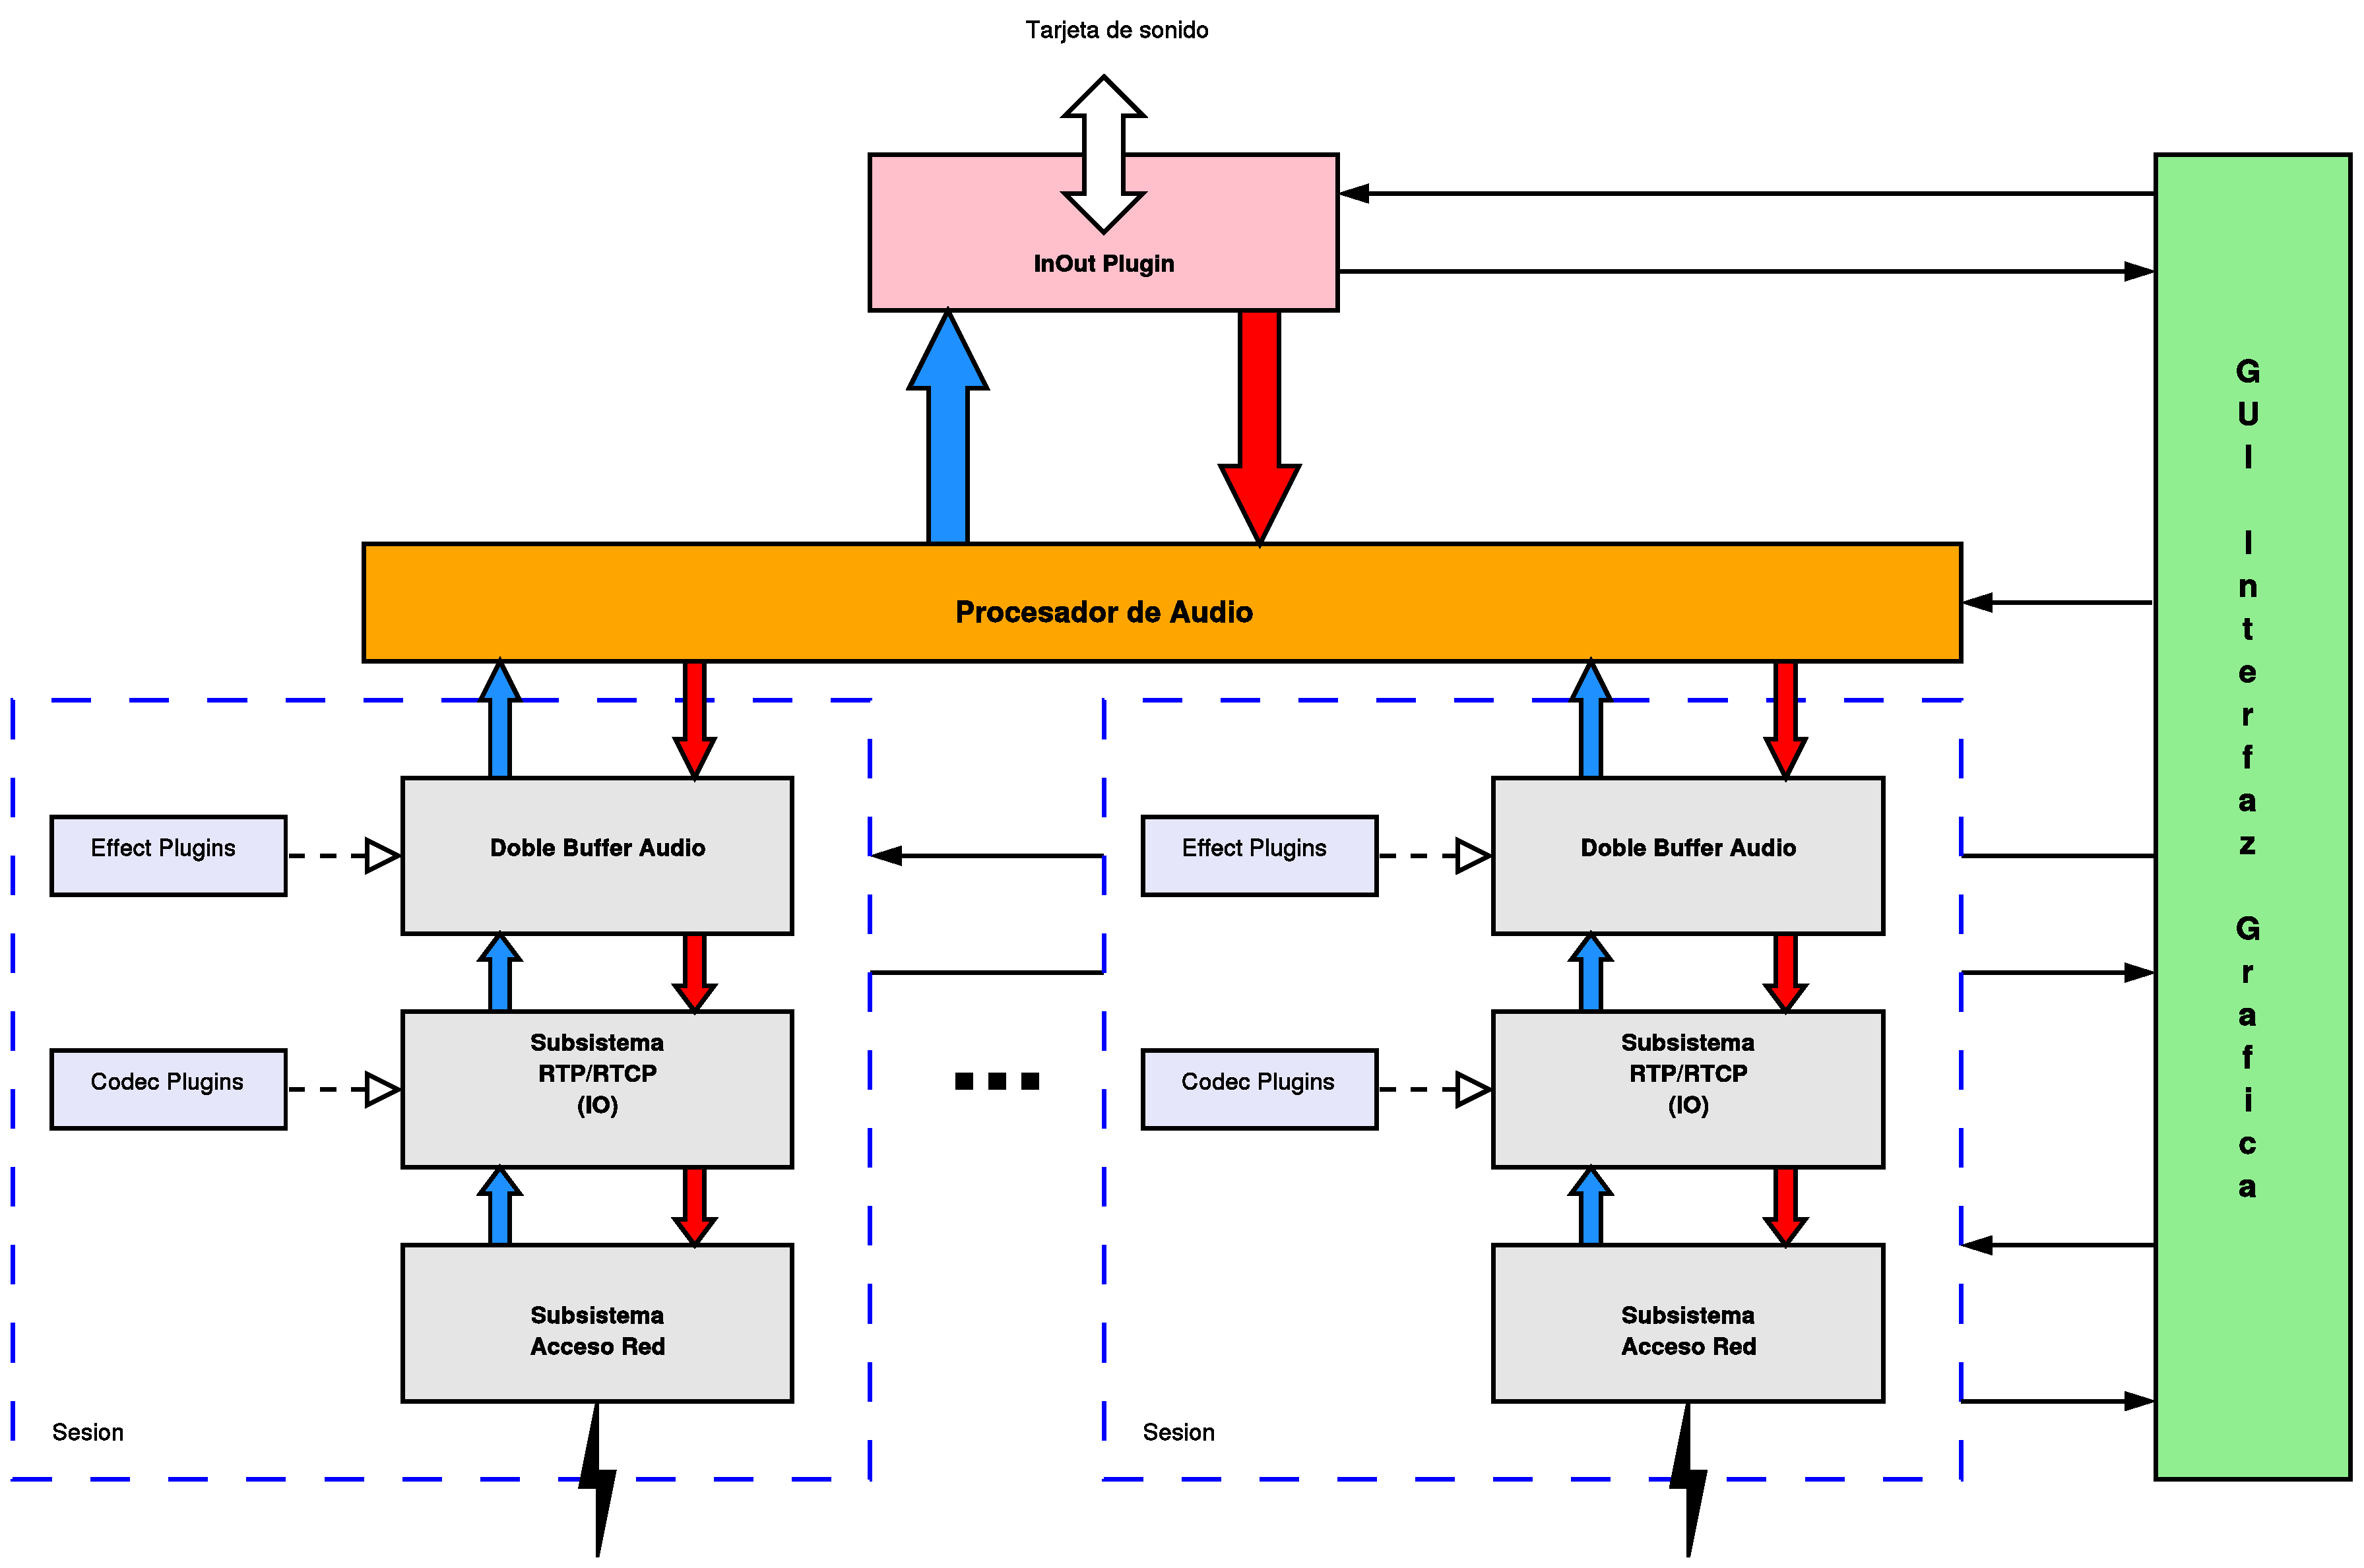
\includegraphics[width=\textwidth, height=9cm] {asubio.eps}
\caption{Subsistemas de \software}
\label{fig:asubio}
\end{figure}

A continuaci�n se analiza el dise�o de cada subsistema por separado, para abordar al final la integraci�n entre todos ellos.

\subsection{Interfaz Gr�fica de Usuario. GUI}

La GUI est� desarrollada �ntegramente en GTK+. Contiene servicios de valor a�adido, como por ejemplo la posibilidad de usar una libreta de direcciones para almacenar las direcciones de contactos. Todas las incidencias (errores, informaciones, advertencias, etc ...) son cuadros de di�logo no bloqueantes, y permiten seguir usando el resto de la aplicaci�n, excepto estas tres ventanas:

\begin{enumerate}
	\item La agenda de contactos.
	\item Di�logo de conexi�n o de llamada entrante.
	\item Ventana de configuraci�n, permite configurar los par�metros que afectan al rendimiento de la aplicaci�n, as� como la configuraci�n de los distintos plugins. Su dise�o est� basado en pesta�as, de esa forma se permite a�adir nuevas caracter�sticas f�cilmente y de manera modular.
\end{enumerate}

Otra ventana muy importante es, la ventana de aceptaci�n de llamada entrante. El usuario puede elegir si aceptar o no la llamada. Esta ventana se muestra en primer plano y en el escritorio activo en donde se encuentre trabajando el usuario. No bloquea el resto de la interfaz gr�fica, pero, s�lo existe una ventana de este tipo, esto significa que, mientras que el usuario no acepta o rechaza la llamanda no podr�n aparecer otras llamadas. En \emph{OO} esto se conoce como patr�n \emph{Singlenton}. \\

Otro aspecto importante es el desarrollo de la interfaz principal de control de sesiones, tambi�n se basa en un sistema de pesta�as, donde una pesta�a representa una sesi�n \emph{RTP}. Cada pesta�a permite mostrar y modificar los par�metros de la sesi�n a la que representa. Par�metros como: control de ganancia, mute del micr�fono, mostrar informaci�n de la sesi�n y los plugins y enmudecer al usuario. \\

Todo el dise�o de la \emph{GUI} es totalmente independiente de la l�gica de la aplicaci�n, siguiendo el patr�n \emph{MVC}. De esta forma ser� muy f�cil modificar o desarrollar en el futuro la GUI u otras GUI's con \emph{QT}, con \emph{NCurses} para consola (sin GUI), etc. Como este dise�o tiene un alto grado de paralelismo, todas las ventanas son creadas desde el bucle principal de GTK, para ello se ha implementado un complejo sistema de sem�foros que controlan los mecanismos de transferencia de datos entre varios hilos de ejecuci�n. 

\subsection{Acceso a red}

Como el sistema debe funcionar tanto en redes IPv4 como IPv6, se desarroll� un sitema que permite abstraer completamente las funciones del API de sockets. Aunque esta parte no se desarroll� usando OO, el siguiente diagrama (\ref{fig:api_red} UML permite representar f�cilmente su estructura. Adem�s, este subsistema, debe proveer funciones para acceder a redes \emph{multicast}

\begin{figure}[htb]
\centering
\includegraphics[width=\textwidth, height=7cm] {uml_red.eps}
\caption{Relaciones l�gicas existentes en el acceso a red}
\label{fig:api_red}
\end{figure}

\subsection{Acceso al fichero de configuraci�n}

Hay un TDA que se encarga del acceso a toda la configuraci�n, carga todos los pares {\it clave}={\it valor} que se encuentran en una secci�n {\it [GLOBAL]} por ejemplo. El fichero de configuraci�n presenta el siguiente formato:

\begin{center}
\begin{boxit}
\begin{verbatim}
[GLOBAL]
rtp_base_port=10000
plugins_inout_dir=/home/riguera/.asubio/plugins/inout/
plugins_codecs_dir=/home/riguera/.asubio/plugins/codec/
plugins_effect_dir=/home/riguera/.asubio/plugins/effect/
contact_db=/home/riguera/.asubio/agenda.ml
program_hostname=192.168.1.2
audio_mic_vol=58
audio_spk_vol=65

[OSS]
audio_device_in=/dev/dsp
mixer_device_in=/dev/mixer
audio_source=0
audio_device_out=/dev/dsp
mixer_device_out=/dev/mixer
volume_control=0
\end{verbatim}
\end{boxit}
\end{center}

El TDA lee el fichero en memoria y por medio de listas enlazadas que contienen los pares clave-valor de una secci�n, se puede mantener en memoria toda la estructura. Adem�s esa estructura incorpora sem�foros binarios que impiden que dos \emph{threads} o hilos, accedan y modifiquen una secci�n al mismo tiempo. De esta forma el TDA se puede usar con hilos concurrentes.

\subsection{Procesador de audio}

Es uno de los subsistemas m�s cr�titos del programa, sus dos tareas principales son repartir el audio de entrada (generalmente del micr�fono) y mezclar el audio de salida (hacia los auriculares o altavoces). Es un sistema aut�nomo, es decir, act�a concurrentemente junto con otros subsistemas y es capaz de realizar las siguientes funciones:

\begin{itemize}
	\item Repartir el audio a todas las sesiones u otros subsistemas que lo soliciten.
	\item Mezclar el audio de distintas fuentes, generalmente sesiones RTP.
	\item Controlar el tiempo de escritura y lectura de bloques de audio. Si se escribe o lee demasiado pronto o demasiado tarde en un dispositivo de audio, se producen {\it buffer overrun} y cortes de audio. Los  {\it buffer overrun} provocan cortes en el audio y una p�rdida de rendimiento global del programa. El {\it Procesador de Audio}, es capaz de controlar el tiempo de forma muy precisa para evitar que se produzcan estas situaciones.
\end{itemize}

\begin{figure}[htb]
\centering
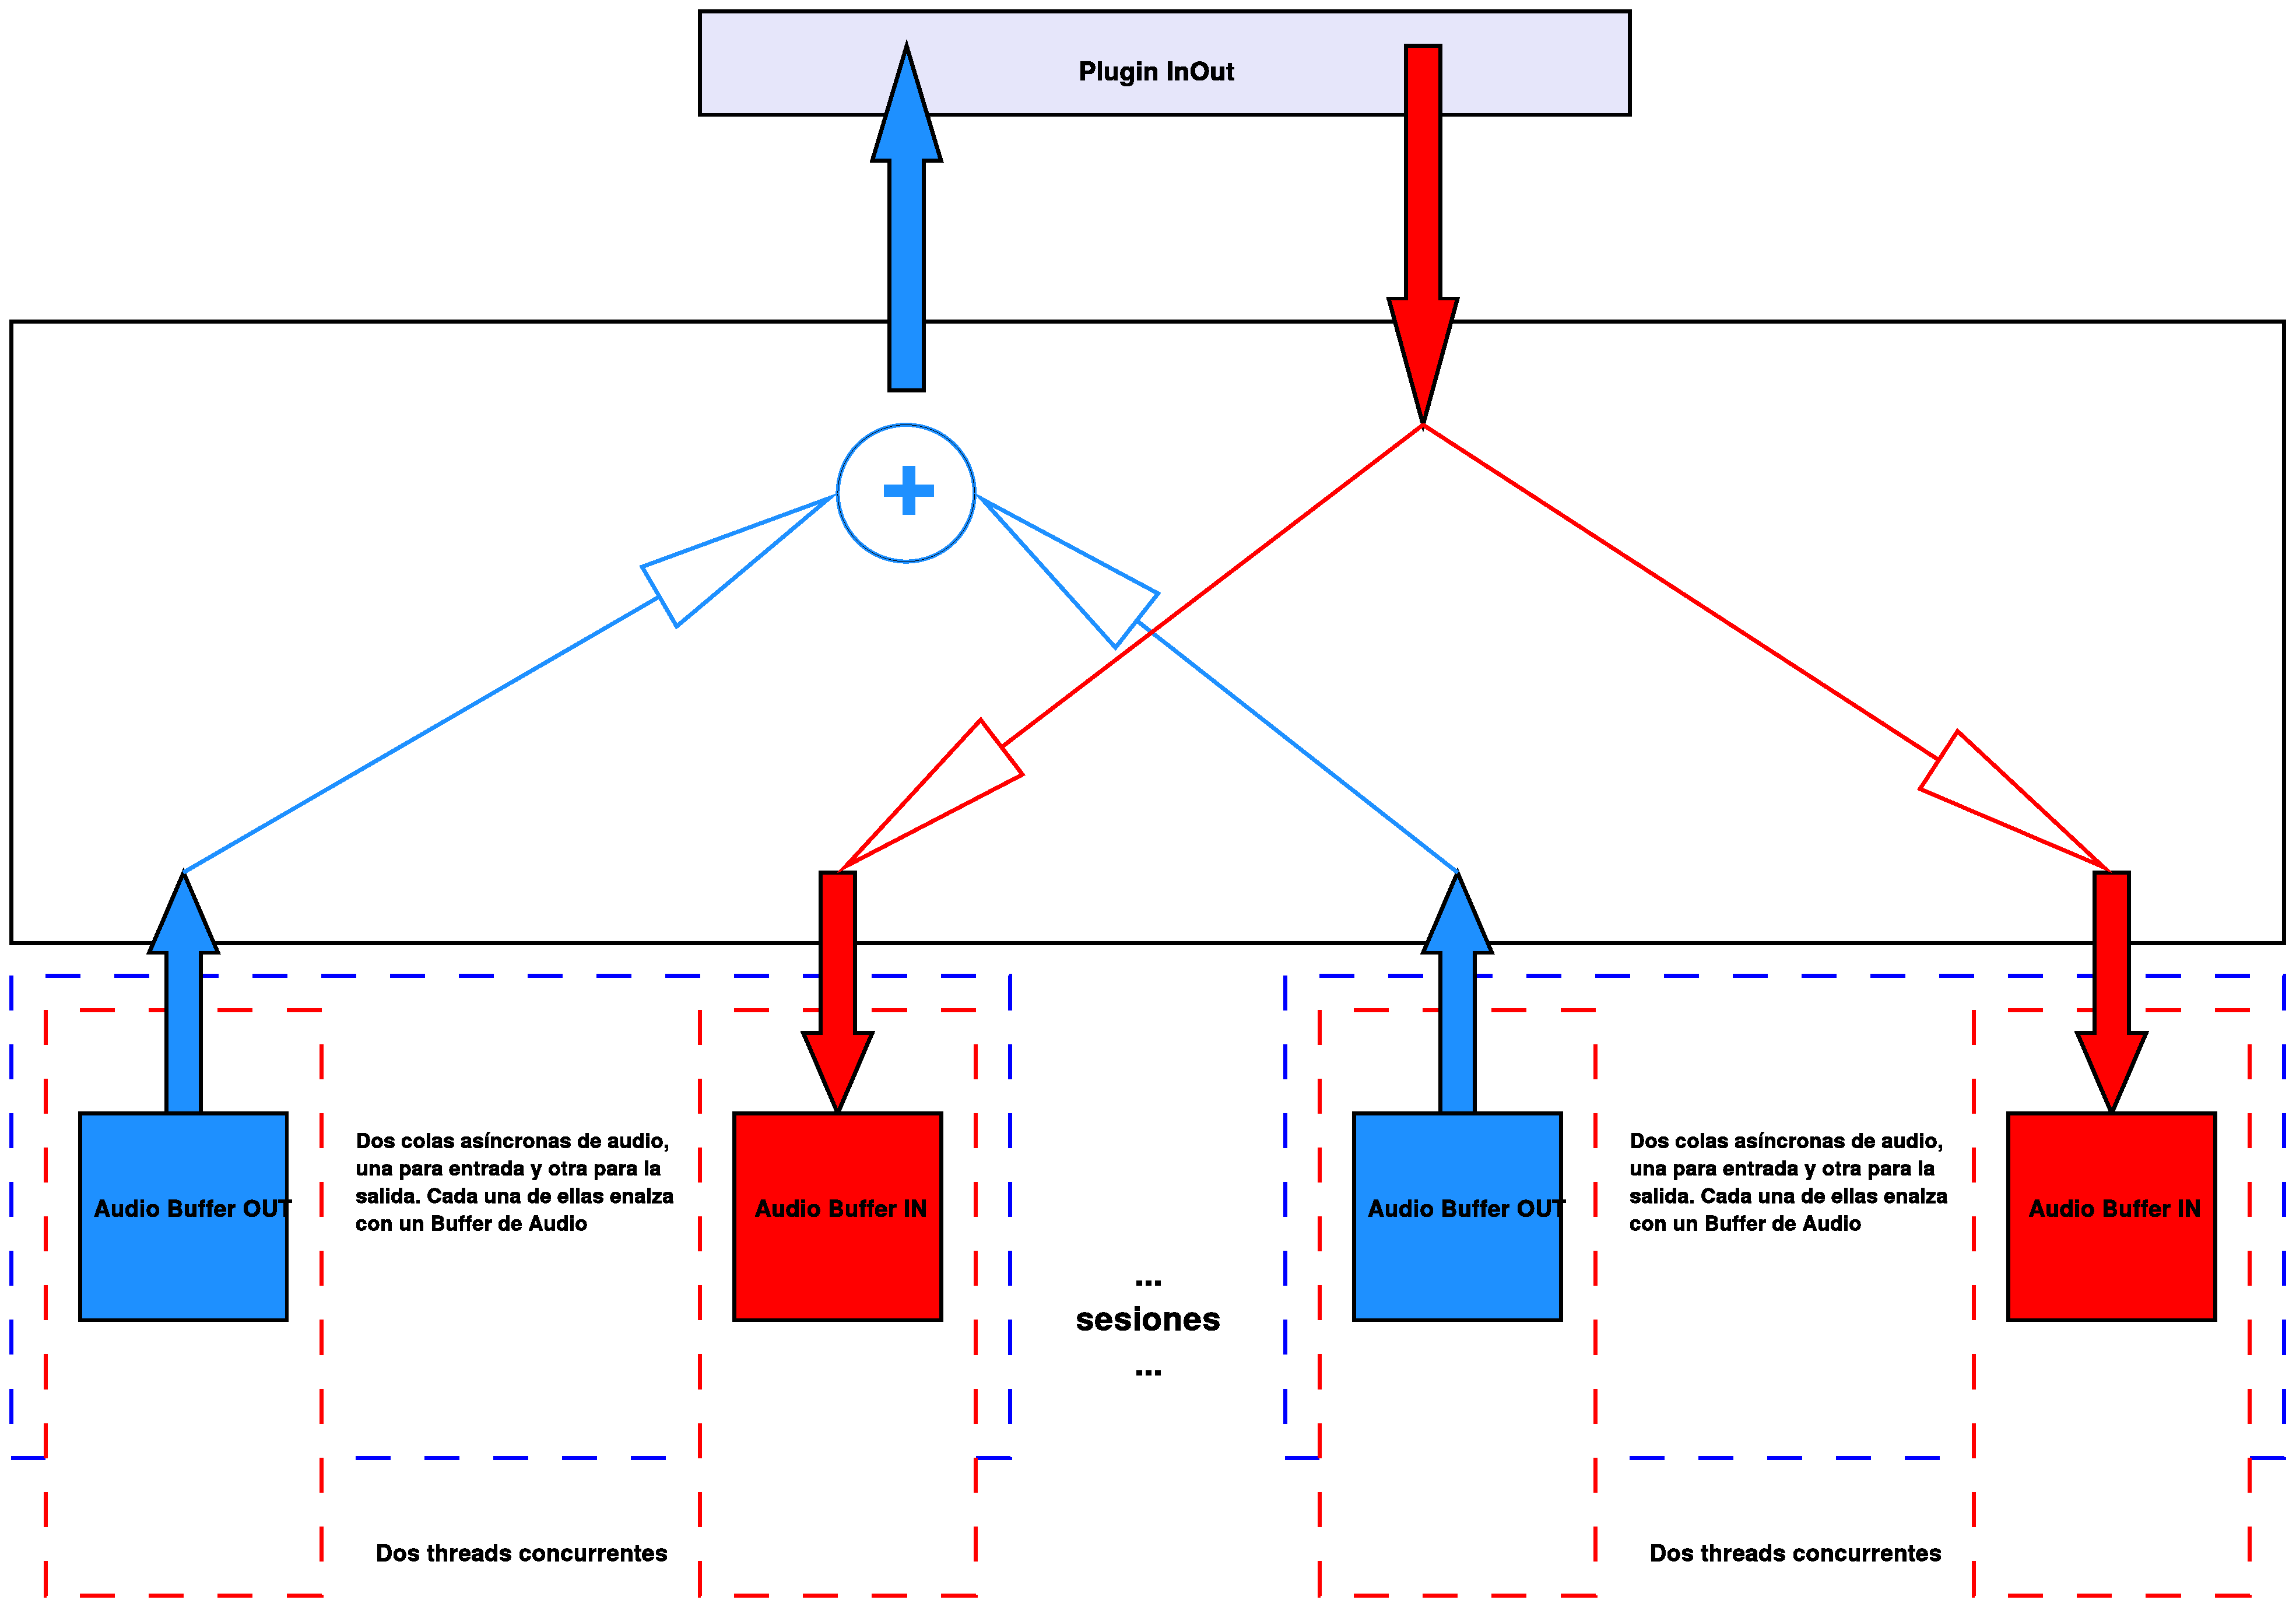
\includegraphics[width=\textwidth, height=9cm] {audio_processor.eps}
\caption{Funcionamiento l�gico del Procesador de Audio}
\label{fig:audio_processor}
\end{figure}

Todo el audio que se maneja en el programa es tratado por este subsistema. Dicho es un \emph{TDA}, aunque en un contexto de patrones se asemajar�a a un \emph{Singlenton}, es decir, no pueden existir dos {\it Procesadores de Audio} en el programa. \\

El audio que despacha o recibe este subsistema, llega a trav�s de un canal as�ncrono -ya que �l se encarga de gestionar el tiempo-. Ese canal tiene propiedades de cola, por lo que si una fuente env�a de repente muchos bloques de audio, los bloques de audio sobrantes, ser�n encolados para su tratamiento posterior, es decir, act�a como un colch�n frente a estas variaciones en la red. Por supuesto, dispone de un sistema de sincronizaci�n para controlar la longitud de esas colas de audio. Los canales de audio tienen tambi�n propiedades bloqueantes, es decir, si no hay bloques para leer en un canal, esa llamada quedar� bloqueada hasta que lleguen datos. \\

Este subsistema est� relacionado estrechamente con el \emph{InOut Plugin}, ya que usa su api, en concreto sus funciones de E/S de audio para interactuar con el dispositivo. Sin embargo no tiene capacidades de inicializar el plugin, es decir, el plugin {\it InOut} ya est� inicializado cuando se ejecuta el {\it Procesador de Audio}. \\

El audio que trata este subsistema se procesa en formato 16 bits, \emph{LITTLE ENDIAN}, mono, muestreado a 8000Hz. Si el sistema en que se ejecuta es \emph{BIG ENDIAN} se deber� recompilar, con compilaci�n condicional, para tratar correctamente el audio.

\subsection{Doble buffer de audio}

Este subsistema tambi�n es muy importante, cada cola de audio que se solicita al \emph{Procesador de Audio} termina en un buffer de audio. Se puede apreciar en la figura siguiente (\ref{fig:audio_buffer}):

\begin{figure}[htb]
\centering
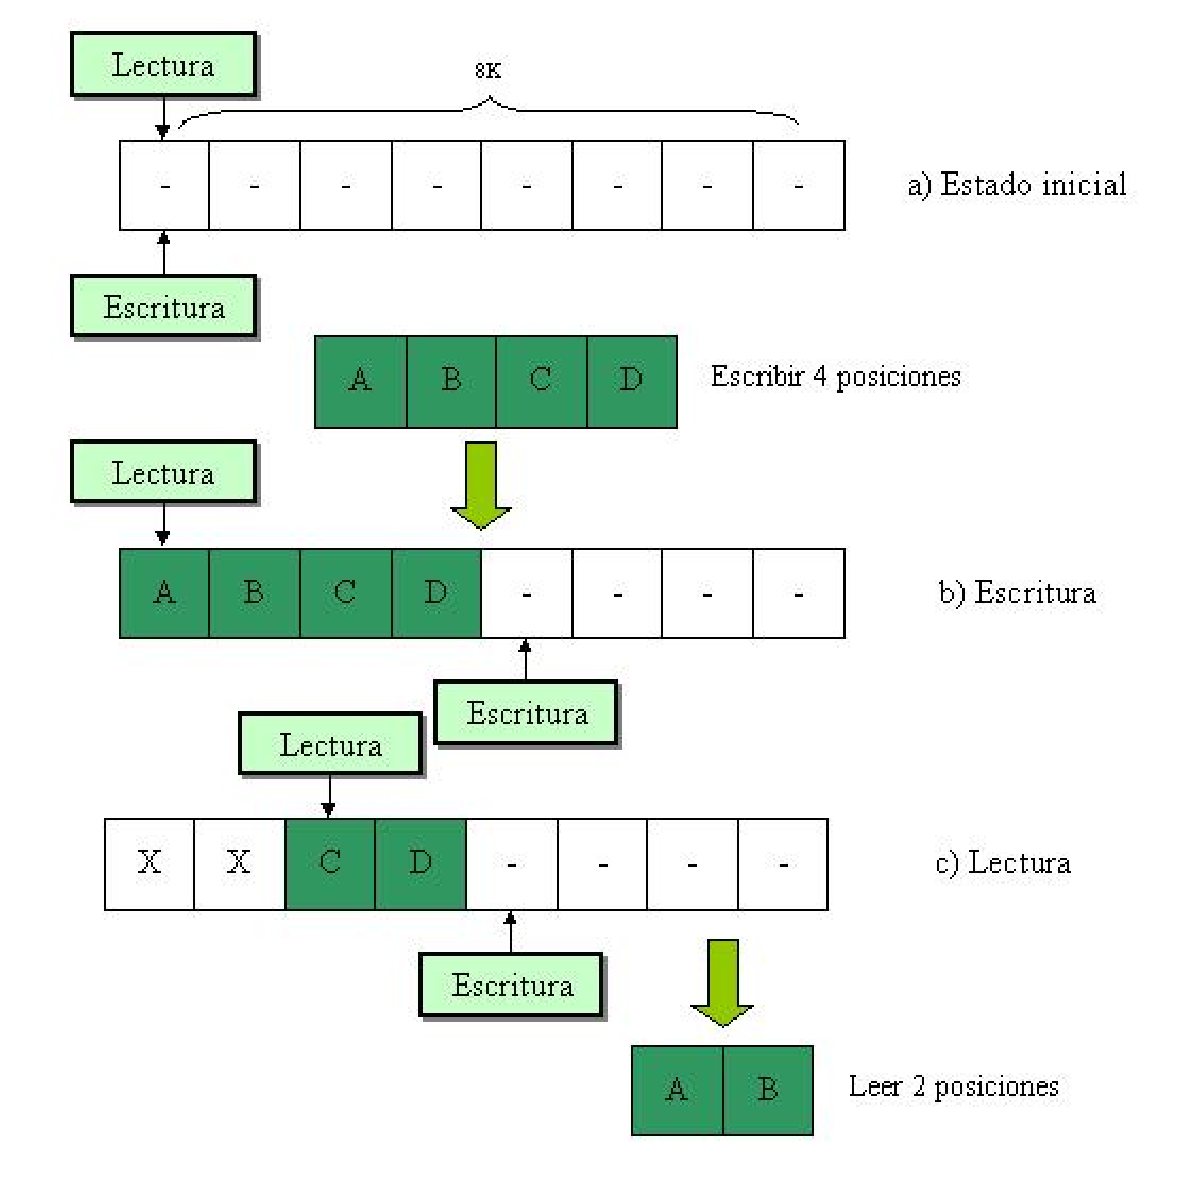
\includegraphics[width=9cm, height=7cm] {buffer_audio.eps}
\caption{Funcionamiento del doble buffer de audio}
\label{fig:audio_buffer}
\end{figure}

La existencia de estos buffers de audio constituye otra parte fundamental de la arquitectura de audio. Se podr�a dise�ar perfectamente un sistema de audio carente de dichos b�fferes, consiguiendo una calidad en el sonido no necesariamente mala. Pero, gracias a los bufferes de audio, se consigue una indepencia l�gica y f�sica del \emph{Procesador de Audio} con el subsistema RTP/RTCP, ya que est�n implementados por hilos diferentes que no tendr�n ninguna relaci�n en com�n. Se iniciar�n y parar�n por separado, y ninguno de los dos (en realidad son tres) tendr� constancia de la presencia del otro. Las ventajas de esta arquitectura son evidentemente, que los problemas en un hilo no afectan al otro, y que al no estar relacionados no se crear�n conflictos entre ambos. El uso de hilos o procesos ligeros junto con los buffers de audio, aporta estas ventajas:

\begin{description}
	\item [Acople de velocidades:] el acople de velocidades entre la lectura/escritura del audio desde el \emph{Procesador de Audio} y la emisi�n/recepci�n de paquetes RTP desde la red. En un dise�o basado en un s�lo hilo que realiza secuencialmente una lista de tareas, el tema del acople de las velocidades puede llegar a suponer grandes dolores de cabeza por dos circunstancias: por una parte, el dispositivo de audio necesita que se le suministre las muestras de audio en una cantidad relativamente abundante (para bloquear lo menos posible el dispositivo y permitir una reproducci�n sin cortes. Es much�simo mejor realizar pocos accesos y manejar m�s datos, que muchos peque�os accesos para peque�as cosas) y de forma constante. Por otra parte, la red es aleatoria y no fiable, ya que son comunes los momentos de silencio en los que no llegar� ning�n dato para, a continuaci�n, llegar todos de golpe.
	\item [Mejora en las posibilidades de acceso:] en un sistema de sonido compuesto por un �nico hilo que acceda al \emph{Procesador de Audio}, codificando/decodificando y accediendo a la red de forma c�clica y secuencial, el usuario y por ende, el sistema de audio, nunca tendr� acceso de ninguna manera a las muestras de sonido. Usando un buffer intermedio se pueden implementar ciertos sistemas, como se mostrar� m�s adelante, para permitir por ejemplo, una lectura no destructiva del buffer. 
	\item [Mayor facilidad para realizar mejoras:] al dividir el problema y acordar una interfaz com�n (el acceso a los b�fferes) es sencillo eliminar una parte y sustituirla por otra. Se puede cambiar el protocolo de transporte de los flujos (RTP) por otro, si as� se estimara oportuno en cierto momento, sin tener que alterar una sola l�nea de las funciones que proporcionan el acceso a los recursos de audio de la m�quina.
	\item [Tama�os de bloque de audio distintos] el uso de los buffers permite que se puedan leer tama�os de bloque distintos del \emph{Procesador de Audio} de los que emplean los codecs de audio.
\end{description}	

\subsection{Plugins}

La adici�n de funciones en tiempo de ejecuci�n elimina la necesidad de modificar el c�digo base. La incorporaci�n de los plugins permite mediante un sistema abierto crear componentes reusables del que pueden ser beneficiarias varias aplicaciones a la vez. Adem�s, los plugins, al ser independientes del programa, permiten incorporar una serie de tecnolog�as propietarias o patentadas que de otra forma ser�a imposible. \\

La carga de plugins es totalmente independiente del sistema sobre el que se ejecute el programa. Glib tiene funciones que permiten abstraer completamente la creaci�n y el uso de plugins en el software. Todos los tipos de plugins deben tener en com�n una �nica funci�n, la que exporte una estructura al programa principal que permita acceder luego a las funciones y s�mbolos del plugin. De ese modo se evitan que las funciones desperdigadas.

\subsubsection{\textbf{{\it InOut}} Plugins}

Su funci�n principal es capturar y escribir el audio en el dispositivo de sonido del PC, es decir, tal como su nombre indica, es el encargado de la entrada-salida de audio en el sistema local. La interfaz de este plugin debe aportar funciones de lectura y escritura de audio, en un dispositivo de audio. Se debe tener en cuenta que el acceso a las funciones de lectura y escritura de audio puede ser full-duplex.

\subsubsection{\textbf{{\it Effect}} Plugins}

Tienen como funci�n expandir el funcionamiento del programa. Estos plugins pueden modificar los flujos de audio de entrada y salida para poder a�adir funcionalidades como. 

\subsubsection{\textbf{{\it Codec}} Plugins}

Son la clave de funcionamiento del programa, su funcion es aportar una m�todo de compresi�n de audio. Estos se implementaron de forma diferente a los anteriores, en este caso existe un objeto llamado {\it codec} del que heredan todos estos plugins. La razones por la que se implementaron de esta forma son:

\begin{itemize}
	\item Facilidad de programaci�n, una vez ``instanciado'' el objeto, basta con llamarlo para los frames de audio de un flujo.
	\item Al emplear la herencia, siempre se usa la misma funci�n, es independiente del nombre del plugin, de su estado, etc.
	\item Futuras ampliaciones del proyecto, como por ejemplo la posibilidad de recomprimir audio para asuntos de recuperaci�n o retransmisi�n.
\end{itemize}

El siguiente diagrama UML modeliza la clase {\it Codec} (figura \ref{fig:vocodec}):

\begin{figure}[htb]
\centering
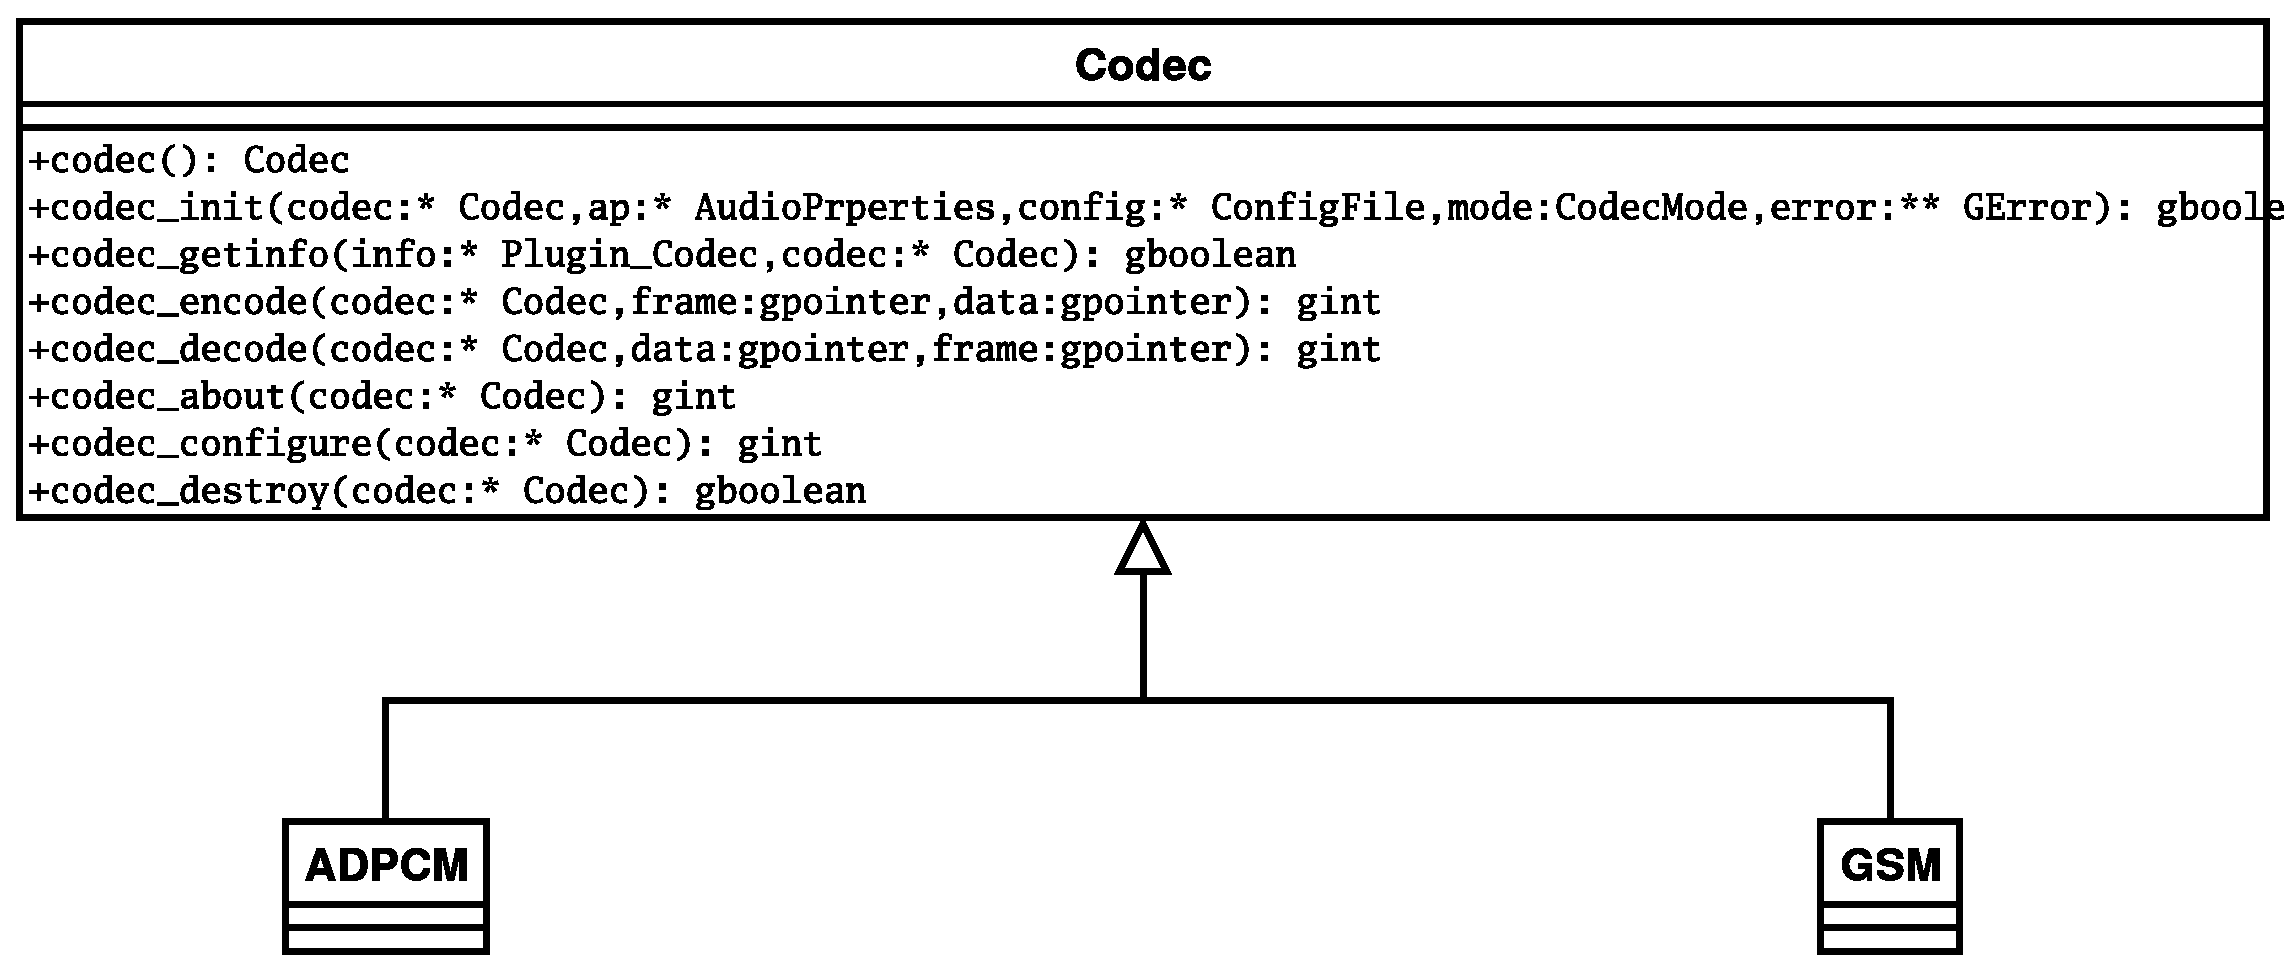
\includegraphics[width=10cm, height=6cm] {codec.eps}
\caption{Diagrama de la clase Codec}
\label{fig:vocodec}
\end{figure}

\section{Concepto de sesi�n}

Una sesi�n es simplemente el estado de una comunicaci�n RTP. Para que el programa sea multisesi�n, aparte de lo ya explicado del subsistema de audio, del GUI, etc. necesita guardar el estado de todas sus sesiones activas. Se implement�, con ayuda de los TDA de Glib, un sistema de lista enlazada que contiene todo lo referente a cada sesi�n. Cada vez que se crea o destruye una sesi�n, se a�ade o borra un estado a la lista. Para obtener cualquier informaci�n de una sesi�n, basta con buscar esa sesi�n en la lista y obtener los datos de los campos significativos. \\

Cuando se crea una sesi�n nueva, lo primero que se hace es comprobar si est� lanzado el {\it Procesador de Audio}, o dicho de otro modo, comprobar si existen otras sesiones activas. Si no se est� ejecutado el {\it Procesador de Audio}, se lanza. Si no funciona o est� ocupado el dispositivo de E/S de audio, -\emph{InOut Plugin}-, se muestra el mesaje de error al usuario. Despu�s se solicita una cola as�ncrona para lectura y otra para escritura del audio al {\it Procesador de Audio}, se aguarda la concesi�n y se contin�a con la creaci�n del proceso RTP/RTCP. Una vez finalizado todo el proceso l�gico correctamente, se crean todos los ``widgets'' en la GUI. Finalmente se a�ade la refencia a esa sessi�n a la lista de sesiones activas.

\subsection{Subsistema RTP/RTCP}

Como se puede apreciar en la figura \ref{fig:io}, este subsitema comprende tres hilos de ejecuci�n. El uno se encarga de recibir los datos de la red, otro de enviarlos y un tercero se encarga de controlar a ambos y de controlar la sesi�n RTCP. Esta forma de distribuci�n de los hilos permite aprovechar al m�ximo el tiempo de CPU concedido. Adem�s, este dise�o, favorece el cumplimiento del est�ndar RTP/RTCP, ya que, de esta forma el hilo RTCP se puede dedicar a controlar los timeouts de los usuarios.

\begin{figure}[htb]
\centering
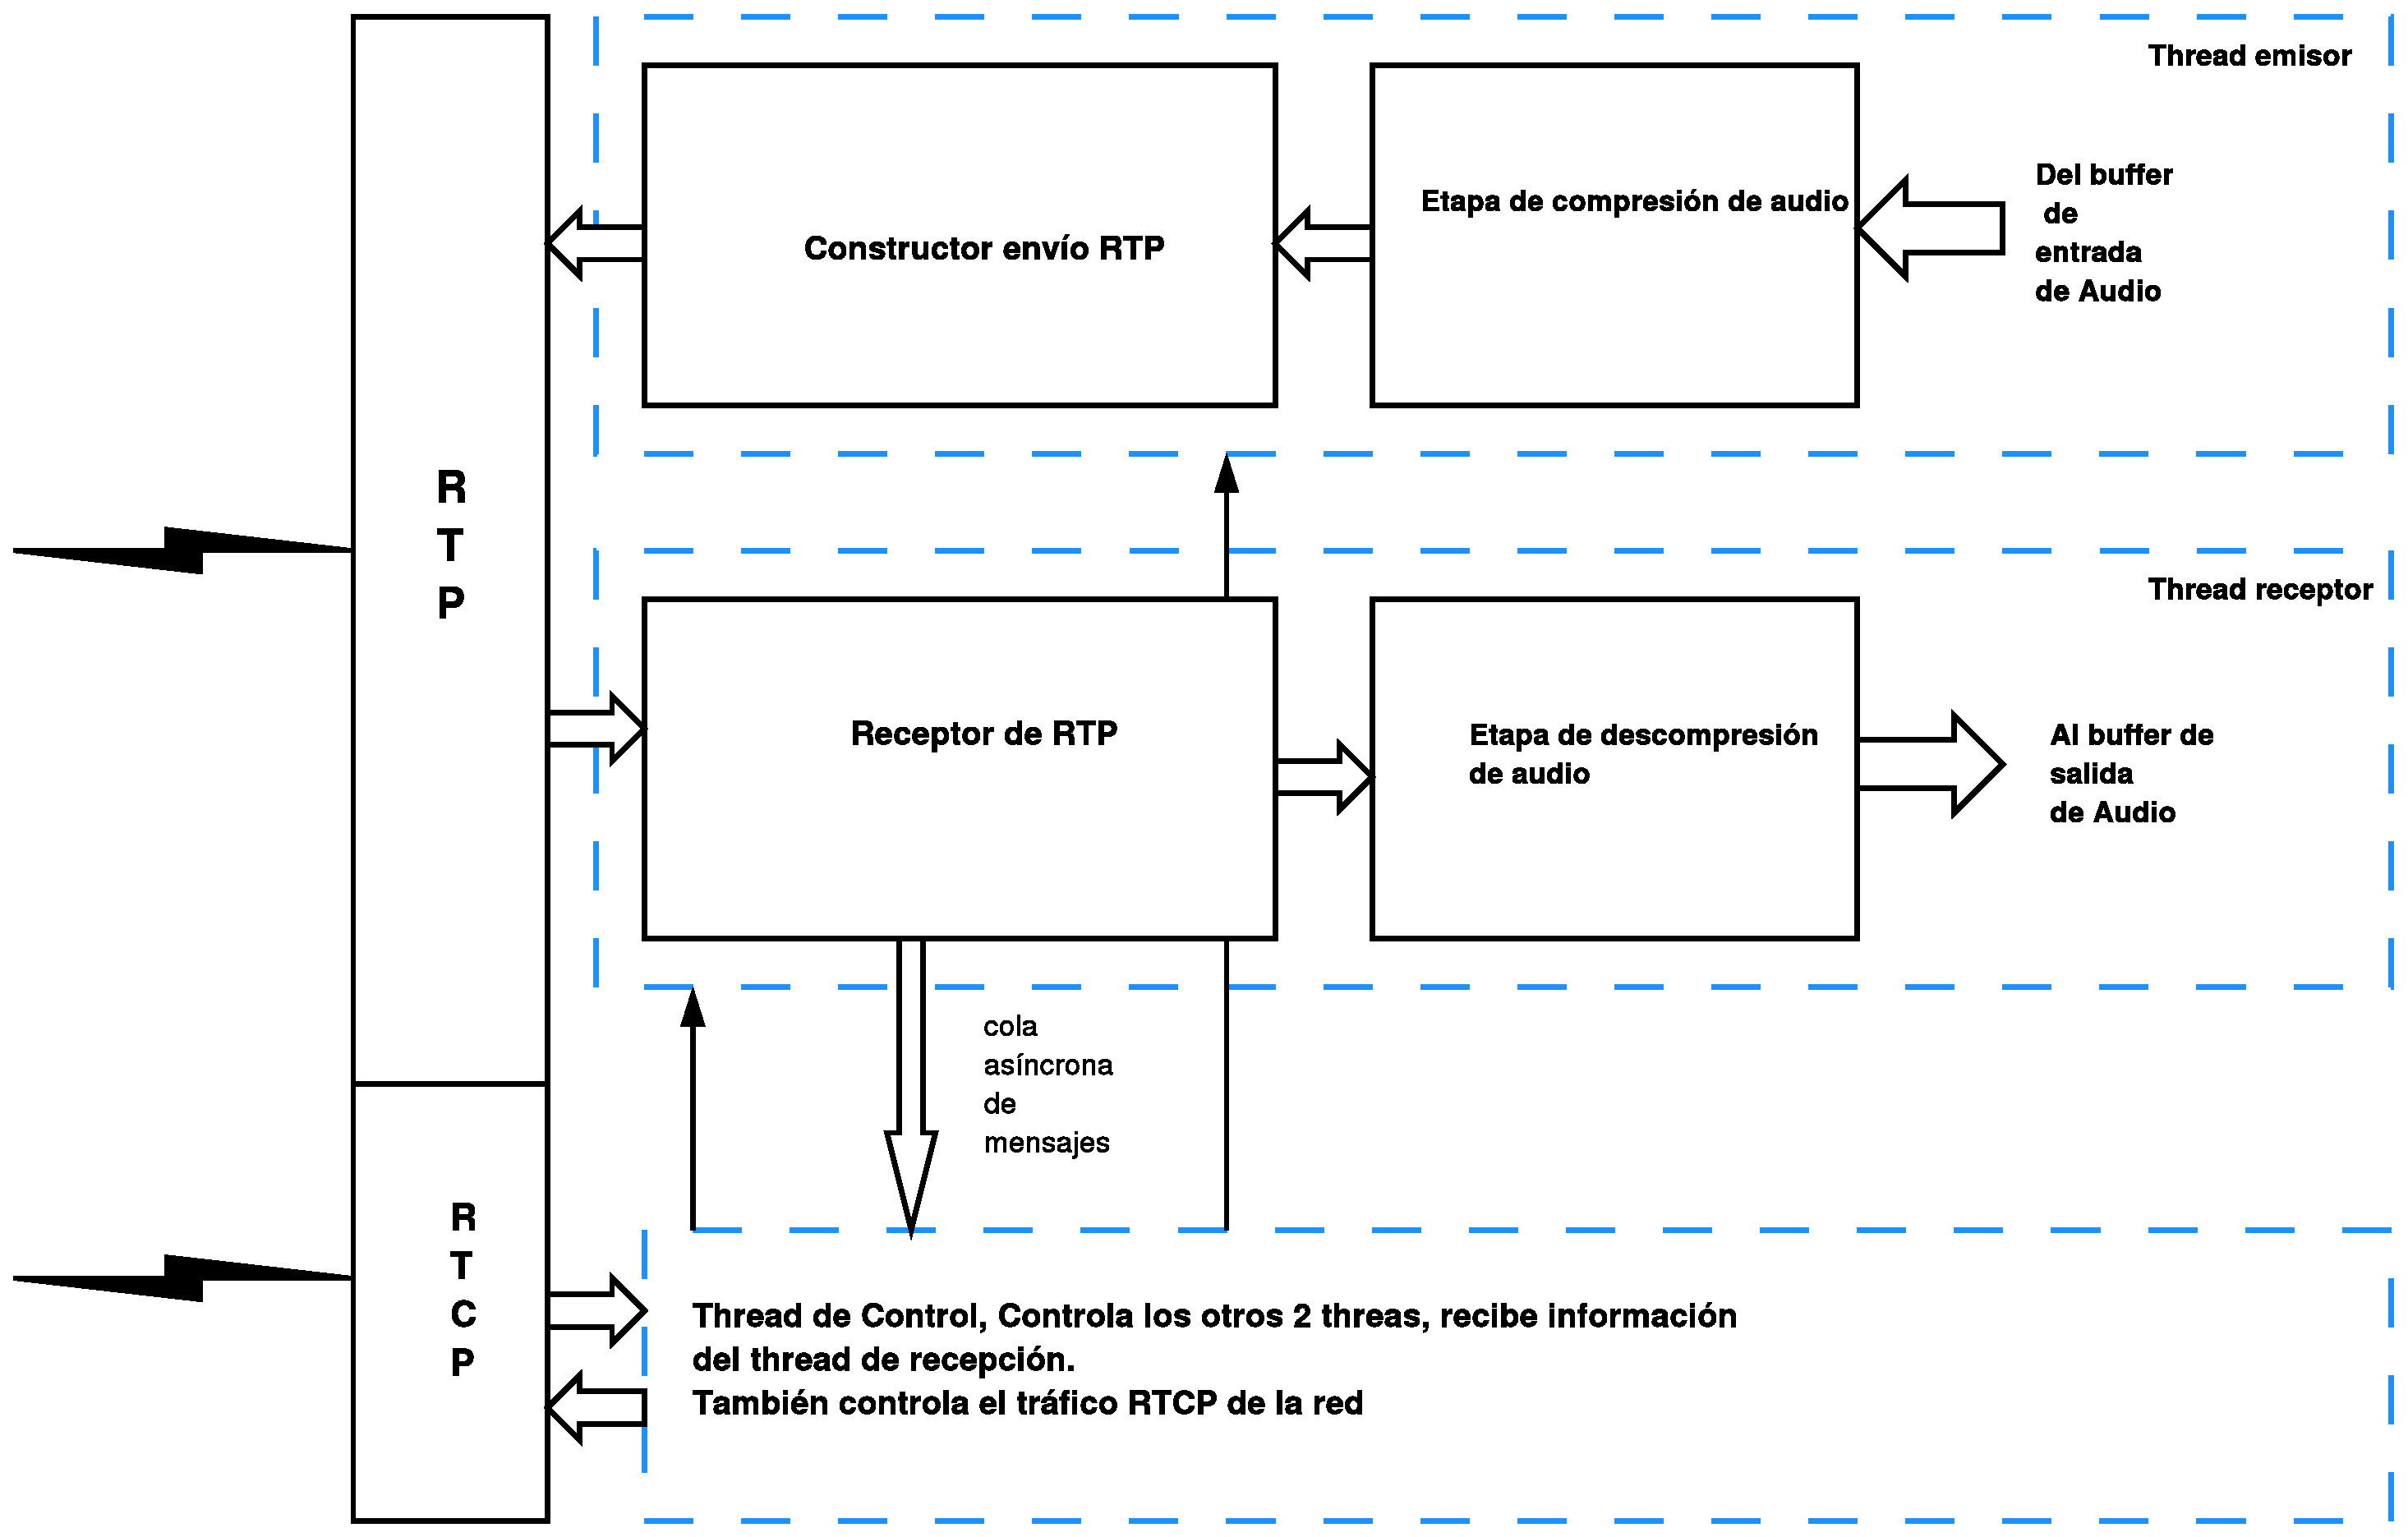
\includegraphics[width=\textwidth, height=9cm] {io.eps}
\caption{Funcionamiento del subsistema IO}
\label{fig:io}
\end{figure}

Hay que tener en cuenta que estos tres hilos acceden concurrentemente a la librer�a de RTP/RTCP, por lo que hay que controlar esta situaci�n con sem�foros.

\section{Simple Session Initiation Protocol. SSIP}

Es el protocolo encargado de la negociaci�n de inicio de sesi�n. El prop�sito es disponer de un protocolo que controle el inicio de sesi�n entre dos usuarios. El funcionamiento es de esta forma:
\begin{enumerate}
	\item El usuario espera las llamadas en un puerto.
	\item Cuando recibe una llamada comprueba que es para �l, en caso contrario se descarta.
	\item Si el usuario que llama est� ignorado en la agenda de contactos, se rechaza la llamada
	\item El usuario debe aceptar o rechazar la llamada, si la rechaza, finaliza la comunicaci�n.
	\item Una vez que se ha aceptado la llamada se negocian los codec que el usuario, que ha iniciado la llamada, ha elegido, si ambos usuarios no tienen codecs coincidentes, finaliza la comunicaci�n.
	\item Tras la negociaci�n de los codecs, se procede a la negociaci�n de los puertos de transmisi�n y recepci�n RTP.
	\item Finalizaci�n de la negociaci�n con �xito.
\end{enumerate}

El diagrama \ref{fig:ssip} ilustra esta negociaci�n:

\begin{figure}[htb]
\centering
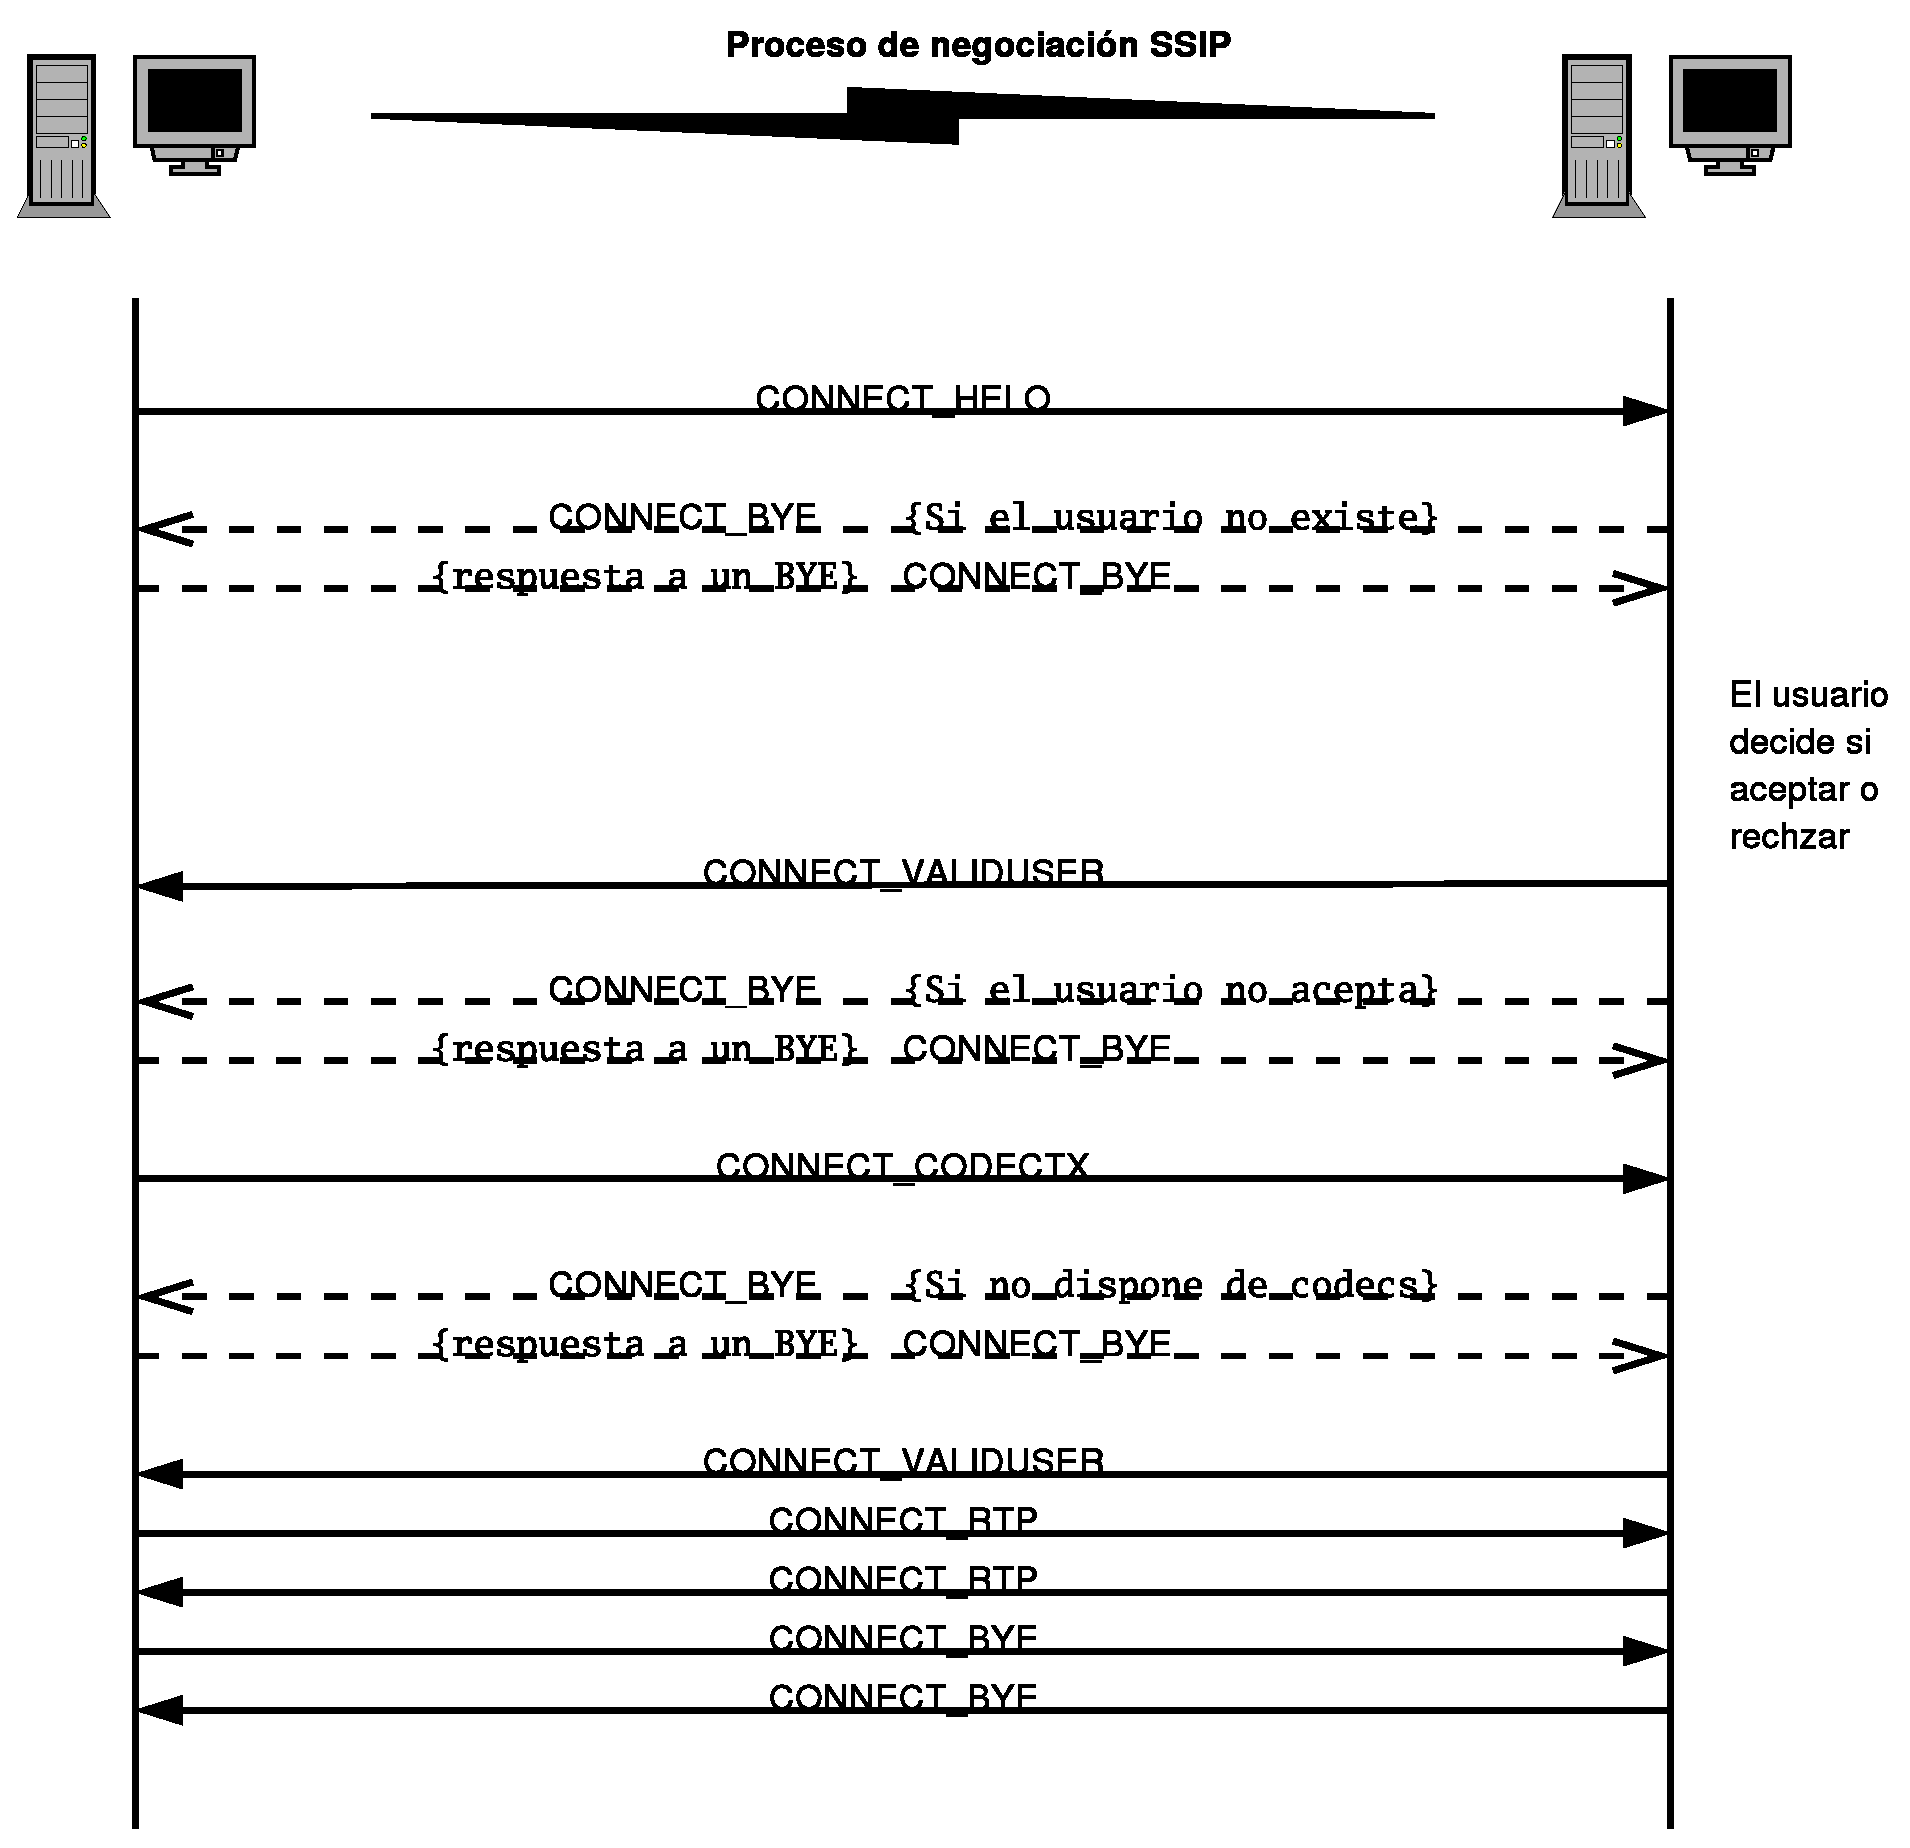
\includegraphics[width=8cm, height=10cm] {SSIP.eps}
\caption{Negociaci�n SSIP}
\label{fig:ssip}
\end{figure}

A continuaci�n se va a detallar todos los tipos de paquetes de SSIP:
\begin{description}
	\item [\emph{CONNECT\_HELO}:] es el primer paquete que se envia para iniciar la negociaci�n. Contiene informaci�n del usuario del que procede y al que va enviado. Soporta el envio de un mensaje de texto de no m�s de 256 caracteres.
	\item [\emph{CONNECT\_VALIDUSER}:] Indica que el usuario existe y ha aceptado la llamada. Si se recibe en este punto un \emph{CONNECT\_BYE} puede significar que el usuario no acepte la llamada o no exista en esa {\it maquina:puerto}
	\item [\emph{CONNECT\_CODECTX}:] Informaci�n de los codes de cada usuario, ordenados por orden de prioridad, se prueba sucesivamente con los codecs elegidos, hasta que se encuentre un codec que tienen ambos. cuando el segundo cliente encuentra una coincidencia, env�a otro paquete \emph{CONNECT\_CODECTX} de vuelta s�lo con la informaci�n de ese codec.
	\item [\emph{CONNECT\_RTP}:] Intercambio de informaci�n para los par�metros de la sesi�n RTP (puertos de TX y RX, etc). El segundo cliente debe responder con otro paquete de ese tipo.
	\item [\emph{CONNECT\_BYE}:] Finalizaci�n correcta de la negociaci�n
\end{description}

Este protocolo presenta unas particularidades:
\begin{itemize}
	\item Como se puede observar, cuando una m�quina env�a un paquete de tipo \emph{CONNECT\_BYE} la otra siempre debe responder, a modo de ping.
	\item La comunicaci�n puede ser interrumpida en cualquier momento con el env�o por cualquiera de las dos partes de un paquete \emph{CONNECT\_ERROR}. Este paquete tiene en le campo DATA, una descripci�n en formato texto del error ocurrido.
\end{itemize}

Los detalles de los campos y de la cabecera de este protocolo se muestran en el cap�tulo de {\it Implementaci�n}.

\section{Proxy SSIP}

Este proceso es el encargado de gestionar el inicio y negociaci�n de sesi�n para un conjunto de usuarios, es decir, aquellos que usen el proxy. Este sistema consta de dos subsistemas: el subsitema de negociaci�n de inicio de sesi�n y el subsistema de control de usuarios. Ambos subsistemas est�n totalmente diferenciados, por lo que son totalmente independientes, excepto en la parte de gesti�n de usuarios, a la que ambos deben acceder para poder realizar su funci�n. La figura  \ref{fig:proxy} muestra gr�ficamente lo comentado. 

\begin{figure}[htb]
\centering
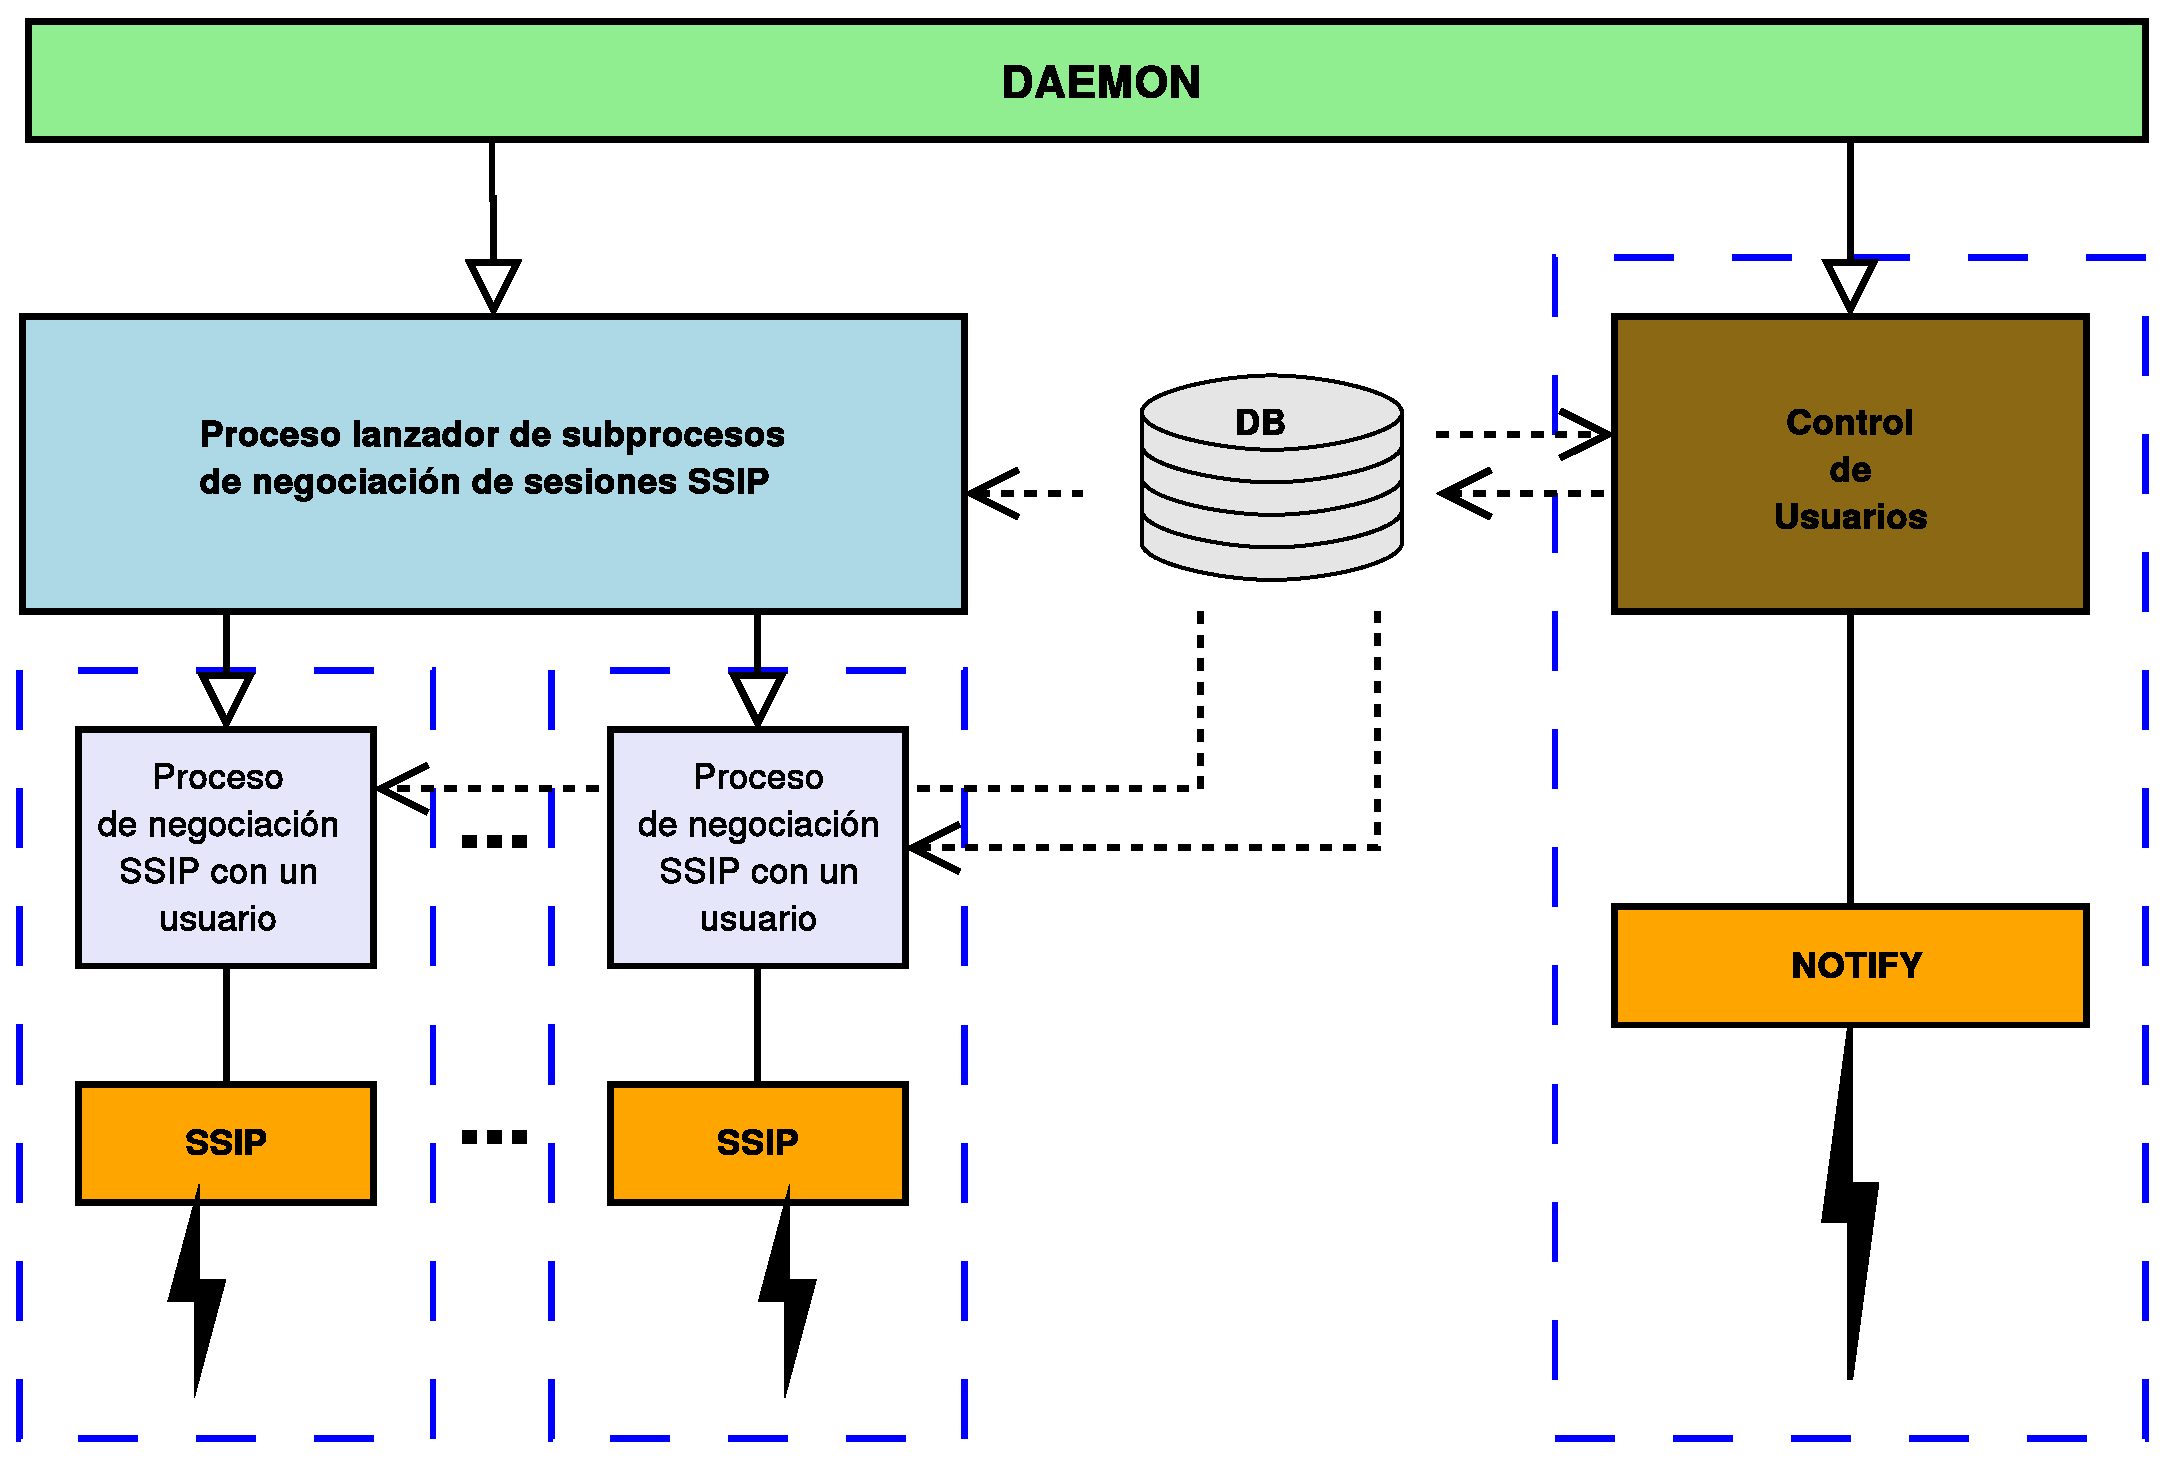
\includegraphics[width=10cm, height=6cm] {proxy.eps}
\caption{Funcionamiento global del proxy}
\label{fig:proxy}
\end{figure}

La gesti�n de los usuarios activos se realiza almacenando sus datos en una base de datos. Como ambos subsistemas son independientes, se opt� por un dise�o concurrente con dos procesos, con un m�todo de control de concurrencia, de otro modo puede ocurrir que, cuando un subsistema acceda al fichero para actualizar los datos de un usuario, el otro subsistema est� leyendo, provocando errores de coherencia en los datos, o incluso errores impredecibles. El dise�o concurrente facilita que se pueda desabilitar c�modamente el subsistema de control de usuarios, manteniendo el otro subsistema funcionando, tal y como se especifica en los requisitos. Tambi�n es necesario implementar un registro de las incidencias de todas las conexi�nes a modo de \emph{log}. El sistema de \emph{logs}, tiene dos opciones (de compilaci�n): imprimir las incidencias por la salida est�ndar o volcarlas al sistema de logs que ofrece Linux (syslog).

\subsection{Configuraci�n}

Todas las opciones que necesita el programa, las lee a partir del fichero de configuraci�n, al arrancar. El fichero de configuraci�n es el �nico par�metro que puede recibir el programa al ser lanzado y debe contener todas las siguientes opciones, todas ellas dentro de la secci�n \emph{[SSIP\_PROXY]}:

\begin{description}
	\item [db\_file]: path absoluto del fichero que va a servir de base de datos de los usuarios del proxy. Si no existe ser� creado.
	\item [username\_manage]: nombre del proxy.
	\item [hostip\_manage]: interfaz de red (direcci�n IP) en la que esperar� las peticiones de negociaci�n de sesi�n SSIP.
	\item [port\_manage]: puerto en que escuchar� el proceso de negociaci�n SSIP.
	\item [num\_forks\_manage]: opci�n de seguridad, indica el n�mero m�ximo (l�mite) de procesos hijo -para atender negociaciones SSIP- que pueden ser creados.
	\item [username\_notify]: nombre del usuario virtual de notificaci�n del proxy.
	\item [hostip\_notify]: interfaz de red (direcci�n IP) en la que ser� lanzado el proceso de control de usuarios con el protocolo \emph{NOTIFY}.
	\item [port\_notify]: puerto en que escuchar� el proceso de contol de usuarios (notificaci�n con el protocolo \emph{NOTIFY}).
\end{description}

A continuaci�n se muestra un ejemplo del fichero de configuraci�n t�pico:

\begin{center}
\begin{boxit}
\begin{verbatim}
#
# SSIP Proxy Configuration file
#
#

[SSIP_PROXY]

db_file=/home/riguera/PROYECTO/ssip_server/users_db.txt

username_manage=ssips
hostip_manage=192.168.1.2
port_manage=40000
num_forks_manage=10

username_notify=ssips
hostip_notify=192.168.1.2
port_notify=30000

\end{verbatim}
\end{boxit}
\end{center}

Para procesar el fichero de configuraci�n, se usa el mismo TDA definido para \software .

\subsection{Subsistema de control de usuarios}

Tambi�n llamado subsistema de notificaci�n. Su funci�n es actualizar la base de datos del proxy, es decir, este subsistema controla los usuarios que emplean el proxy. Cada vez que un usario lanza su programa \software , �ste notifica al proxy que el usuario ya est� online y listo para recibir llamadas. En la notificaci�n se env�a el nombre del usuario, el nombre su m�quina y el n�mero de puerto SSIP (de ese usuario) en donde recibir las conexiones de negociaci�n. Para �sta tarea se cre� el protocolo \emph{NOTIFY}. \\

La base de datos en donde se almacenan los usuarios del proxy, es el mismo TDA usado para la configuraci�n de  \software . Se opt� por esa soluci�n porque: cumple con los requisitos establecidos, se reutiliza el c�digo y presenta una velocidad de proceso aceptable. El siguiente ejemplo muestra c�mo es la base de datos por dentro:

\begin{center}
\begin{boxit}
\begin{verbatim}
[riguera]
host=192.168.1.2
port=10000
password=3jjlvwn
\end{verbatim}
\end{boxit}
\end{center}

De esta forma, un administrador, puede editar f�cilmente el fichero y borrar o inutilizar a determinados usuarios. Los resultados del ejemplo son interpretados de esta forma: \\

El usuario ``riguera'' se encuentra en el host ``192.168.1.2'' esperando negociaciones SSIP en el puerto $10000$. El tercer campo es el ``password'' que aport� el usuario al iniciar su sesi�n con el proxy. Para que este usuario pueda borrar su registro en el proxy, deber� aportar el mismo ``password''. Esto es asi, para evitar que usuarios malintencionados borren a otros usuarios del proxy, lo cual provocar�a que nunca podr�an recibir llamadas.

\subsubsection{Protocolo NOTIFY}

Se desarroll� a partir de SSIP. Descripci�n de los campos de NOTIFY, de los paquetes que se envian al proxy:

\begin{description}
	\item [\emph{IPMODE}:] determina si el paquete contiene direcciones ip de IPv6 o IPv4. El valor de este campo modifica el tama�o de toda la estructura del paquete.
	\item [\emph{FROM\_USER}:] contiene el identificador de usuario que env�a el paquete.
	\item [\emph{FROM\_ADDR}:] direcci�n IP del host en que se encuentra el usuario que ha enviado el paquete.
	\item [\emph{FROM\_PORT}:] n�mero de puerto SSIP en el que se negociaran las sesiones para el usuario con el protocolo SSIP en su host.
	\item [\emph{TO\_USER}:] identificador al que va dirigido el paquete. Est� reservado para futuro uso, para diferenciar distintos proxys. En esta versi�n el contenido de este campo es irrelevante.
	\item [\emph{TO\_ADDR}:] contiene la direcci�n IP del proxy al que va dirigido el paquete.
	\item [\emph{TO\_PORT}:] puerto del proxy al que va dirigido el paquete NOTIFY.
	\item [\emph{DATA}:] contiene una contrase�a generada aleatoriamente, que el proxy almacenar� en su base de datos.
	\item[ \emph{TYPE}:] identifica el tipo de paquete.
\end{description}

El contenido de todos los campos \emph{FROM\_*} y \emph{TO\_*} de los paquetes NOTIFY que se reciben del proxy es el mismo que se envia -si todo transcurre correctamente-, pero permutado, es decir, los campos TO\_* contendr�n el valor que se hab�a enviado antes en los campos FROM\_* y viceversa. \\

En esta parte no es necesario indicar el tama�o de los campos, ya que es el dise�o l�gico. Adem�s el tama�o var�a, dependiendo de si los campos de las direcciones IP contienen IPv6 o IPv4. En el cap�tulo () se mostrar� como se solucion� el problema de conflitos entre IPv4 e IPv6. \\

NOTIFY, dispone de los siguientes tipos de paquetes (campo TYPE), dependiendo del tipo de paquete, la informaci�n del resto de los campos puede cambiar de significado:

\begin{description}
	\item [\emph{USER\_HELO\_ONLINE}:] es el primer paquete que env�a \software al proxy. Su misi�n es indicar que el usuario ya est� online y listo para recibir llamadas.
	\item [\emph{USER\_OK\_ONLINE}:] es la respuesta que envia el proxy, cuando se le ha enviado un \emph{USER\_HELO\_ONLINE}, para indicar que el proceso ha ido bien y ese usuario ha sido a�adido a la base de datos. 
	\item [\emph{USER\_BYE\_ONLINE}:] se env�a para indicar que el usuario se da de baja en el proxy. Su misi�n es indicar que el usuario no est� online y no va a admitir llamadas.
	\item [\emph{USER\_OK\_OFFLINE}:] es la respuesta que env�a el proxy tras un USER\_BYE\_ONLINE para indicar que el proceso ha ido bien y ese usuario ha sido dado de baja.
	\item [\emph{USER\_INCORRECT}:] es la respuesta que envia el proxy tras un USER\_HELO\_ONLINE o un USER\_BYE\_ONLINE.  Si el proxy lo env�a tras recibir un USER\_HELO\_ONLINE, significa que ya existe un usuario en la base de datos con el mismo nombre. Si es enviado tras un USER\_BYE\_ONLINE, se puede dar una de estas dos situaciones:
		\begin{enumerate}
			\item Que el usuario no exista en la base de datos.
			\item Que la contrase�a para ese usuario, indicada en el campo DATA, no sea la misma con la que inici� la sesion, en este caso, el usuario no ser� borrado de la base de datos, continuando online.
		\end{enumerate}
	\item [\emph{ERROR\_PKT}:] este paquete lo env�a el proxy cuando ocurre un error grave e inesperado (no encuentra la base de datos, no hay espacio en disco, etc.) y no puede llevar a cabo la operaci�n solicitada por el paquete que ha recibido de \software . En este caso, en el campo DATA, se env�a un \emph{string} con la descripci�n del problema o error que motiv� el fallo.
\end{description}

El contenido de todos los campos FROM\_* y TO\_* de los paquetes NOTIFY que se reciben del proxy es el mismo que se ha sido enviado, pero permutado, es decir, los campos TO\_* contendr�n ahora el valor que se hab�a enviado antes en los campos FROM\_* y viceversa. NOTIFY funciona de forma simple, es un protocolo que s�lo contiene dos transacciones: el cliente \software envia un paquete y el proxy siempre debe responder con otro paquete y fin de la transacci�n. El cliente siempre es el encargado de iniciar la conexi�n y el proxy de terminarla. \\

\subsubsection{Funcionamiento}

Debido que este subsistema no va a presentar mucha sobrecarga -un usuario s�lo se notifica al darse de alta en el proxy o al abandonarlo- y las transaciones son muy cortas -s�lo dos paquetes NOTIFY-, se ha dise�ado para que atienda las notificaciones secuencialmente, es decir, hasta que no haya finalizado una notificaci�n, no atiende a otra, lo que implica que no hay procesos concurrentes dentro del subsistema. Hay que considerar la posibilidad de que se quede \emph{colgada} (a medias) una transacci�n, como este subsistema es secuencial, si esto ocurre, se bloquear�a todo el proceso de control de usuarios.

El funcionamiento de este subsistema transcurre de este modo:

\begin{enumerate}
	\item El proceso recibe un paquete NOTIFY procedente de un cliente. Si no es de tipo USER\_HELO\_ONLINE o USER\_BYE\_ONLINE o no reconoce el formato, se ignora y finaliza.
	\item Si el paquete NOTIFY es de tipo USER\_HELO\_ONLINE, se busca el usuario en la base de datos. Si el usuario ya existe se constesta con un paquete USER\_INCORRECT, en otro caso se almacena sus datos (usuario, host, puerto y clave) en la base de datos y se contesta con un paquete de tipo USER\_OK\_ONLINE.
	\item Si el paquete NOTIFY es de tipo USER\_BYE\_ONLINE, se busca el usuario en la base de datos. Si el usuario existe y la clave del paquete coincide con la almacenada en la BD, se constesta con un paquete USER\_OK\_OFFLINE y se borran todos los datos de la BD. En otro caso se constesta con un paquete de tipo USER\_INCORRECT y la BD no se modifica.
	\item Si durante el proceso de notificaci�n se produce alg�n error en el proxy, se env�a al cliente un paquete de tipo ERROR\_PKT, con el mensaje de error en el campo DATA.
\end{enumerate}

\subsection{Subsistema de negociaci�n}

Este subsitema se encarga de la negociaci�n SSIP del inicio de sesi�n. Es, realmente, la parte que act�a de proxy, ya que canaliza la comunicaci�n entre el programa cliente (del usuario que llama) y el programa servidor (programa del usario al que se dirige la llamada -con el que se desea contactar-). El proceso de negociaci�n es totalmente transparente para el usuario que inicia la llamada (figura \ref{fig:proxy2}). 

\begin{figure}[htb]
\centering
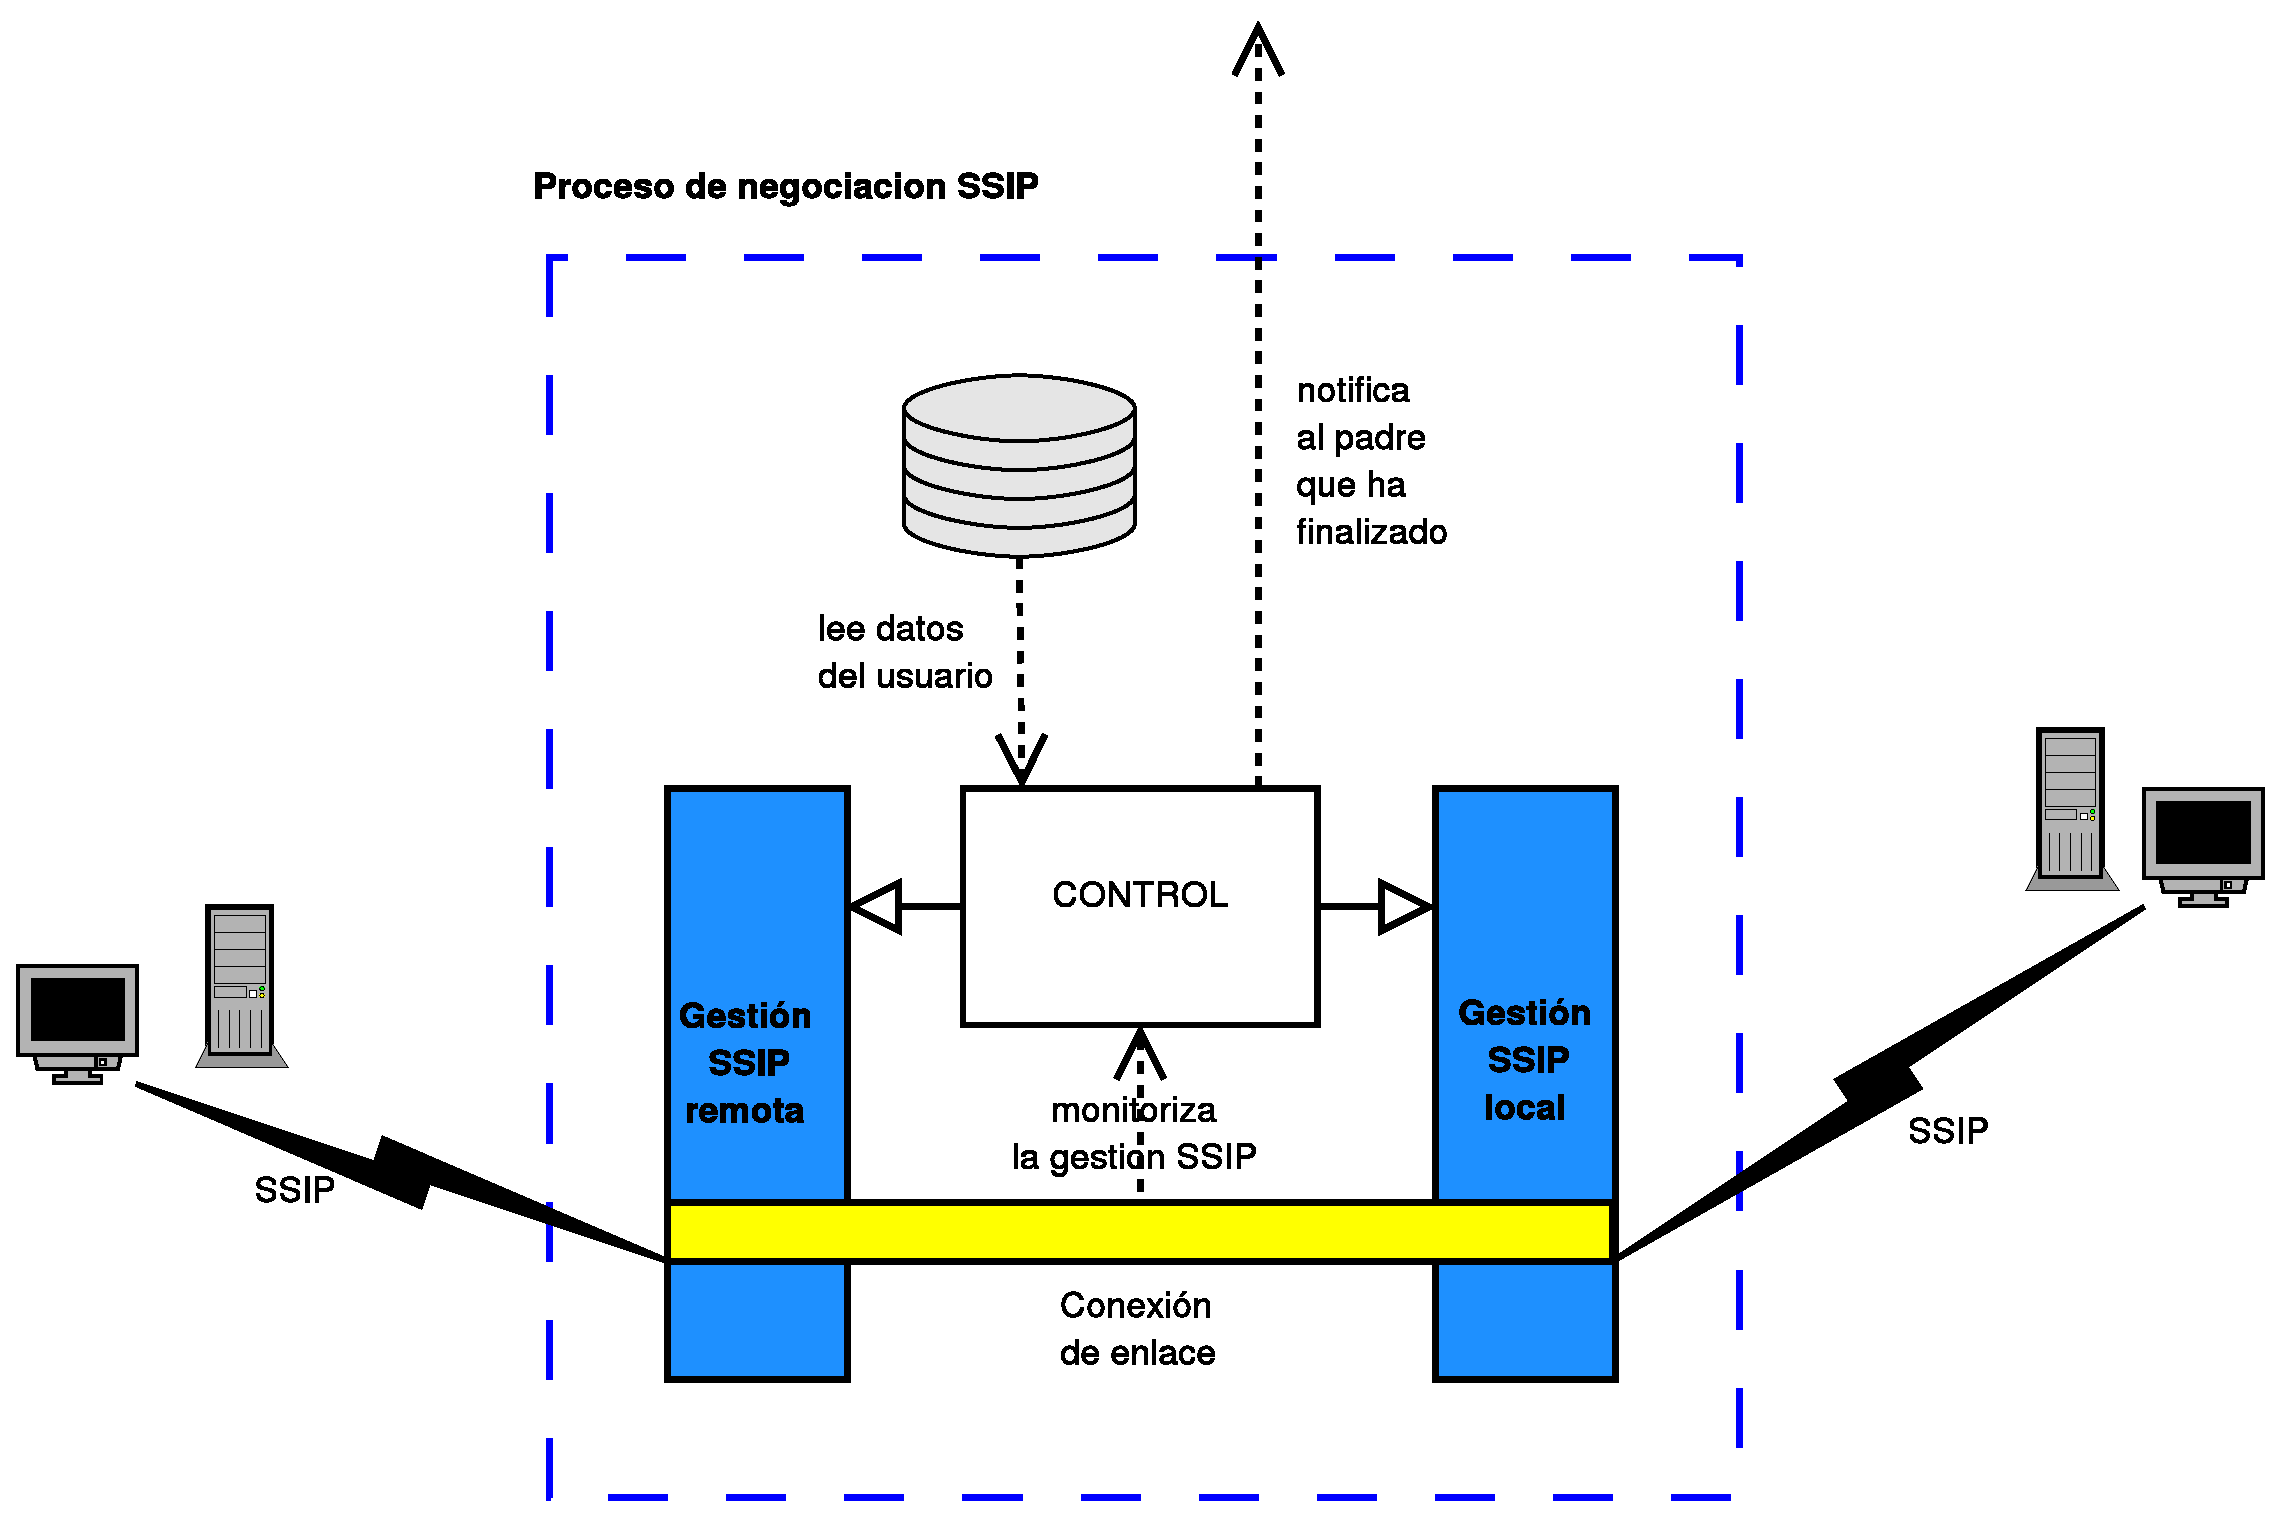
\includegraphics[width=11cm, height=7cm] {neg_SSIP.eps}
\caption{Negociacion SSIP a trav�s del proxy}
\label{fig:proxy2}
\end{figure}

El proceso de negociaci�n con proxy es compatible con la negociaci�n sin proxy, es decir sigue el mismo diagrama de estados mostrado anteriormente en la figura (). Sucede de la siguiente forma:
\begin{enumerate}
	\item El cliente env�a un paquete SSIP de tipo CONNECT\_HELO, que contiene informaci�n del usuario que realiza la llamada. En el paquete se indica el usuario con el que contactar y el host en donde est�, que en este caso es el proxy.
	\item El proxy recibe el paquete, comprueba que es de tipo CONNECT\_HELO, y busca el usuario en su base de datos, si no lo encuentra, le reenv�a al cliente un CONNECT\_BYE y finaliza la comunicaci�n.
	\item Si el usuario existe en ese �mbito (est� en la base de datos), el proxy obtiene los datos necesarios del usuario al que se dirige la llamada, es decir, obtiene el puerto y el host real. Crea una conexi�n con el programa del cliente llamado, que actuar� como servidor, y le env�a el paquete SSIP con el que se inicio todo este proceso.
	\item Si el servidor (programa del cliente al que se llama) responde con un paquete CONNECT\_VALIDUSER, el proxy crea un canal de comunicaci�n bidireccional entre ambos programas. A partir de este momento el proxy, s�lo se limita a actuar de enlace hasta que finalize la comunicaci�n, suceda un error u ocurra un timeout. En el caso de que ocurra un ``timeout'', antes de cortar la comunicaci�n, se env�a un CONNECT\_ERROR al otro canal de enlace.
\end{enumerate}

Como se puede apreciar, el proxy enmascara a todos los usuarios que contiene en la base de datos. Otra consideraci�n que se ha tenido en cuenta es la carga de este subsistema. Al contrario que ocurre con el subsistema de negociaci�n, atiende las peticiones secuencialemente -sin crear otros procesos hijos-, este subsistema crea un proceso hijo para cada petici�n que atiende.

\subsection{Control de concurrencia}

En este sistema no hay \emph{threads}, s�lo hay -como m�nimo- dos procesos concurrentes que acceden a la base de datos. Para el control de concurrencia entre ambos procesos, en el acceso al fichero de la base de datos, el demonio \emph{Proxy SSIP} crea un fichero ``.lck'' -vac�o- que se bloquea para lectura o escritura por cada proceso concurrente, el tipo de bloqueo de este fichero, determina la operaci�n que est� teniendo lugar con el fichero de la base de datos de los usuarios. 

\subsection{Seguridad}

Todo el \textbf{Proxy SSIP}, est� dise�ado teniendo en mente consideraciones de seguridad, por esa raz�n se realizan continuamente controles de datos y longitud de campos de los paquetes recibidos, ``logeando'' cualquier operaci�n sospechosa mediante \emph{syslog}. Pese a que este proceso no necesita privilegios especiales en el sistema -por esa raz�n se recomienda ejecutarlo como un usuario normal, no privilegiado- el lugar que ocupa en la red -en una pasarela o gateway- lo hace un blanco f�cil para distintos tipos de ataques (overflow, DoS, etc.). Tambi�n dispone de un control de n�mero procesos hijo, para evitar ataques de \emph{DoS} (Denegaci�n de Servicio), de forma que s�lo permite que existan como maximo el n�mero de hijos que se indique en el fichero de configuraci�n.



\capitulo{Implementaci�n}
\label{chp:implementacion}
\minitoc
\newpage

Como ya se coment� anteriormente, la implementaci�n del sistema se realiz� en C, porque es un lenguaje que genera ejecutables relativamente r�pidos, lo cual es especialmente interesante en dominios como �ste, donde hay que manejar datos en tiempo real. \\

Adem�s, el sistema en el que se implement� el dise�o ha sido \emph{Linux}, pero, con las herramientas y bibliotecas utilizadas, ambos programas deber�an compilar, casi sin cambios, en cualquier otro sistema que cumpla el est�ndar \emph{POSIX}, incluso en sistemas \emph{MS Windows} contruyendo un plugin para acceder al audio y cambiando el API de Sockets por el WinSock. Esto ser�a realmente dif�cil de conseguir realizando la implementaci�n sobre un sistema cerrado, donde a veces resulta dif�cil saber si se est�n utilizando herramientas o librer�as existentes s�lo para ese sistema. \\

En el presente cap�tulo se mostrar�n fragmentos de c�digo fuente del software implementado, comentando los aspectos m�s significativos, de otro modo, resultar�a imposible comentar en esta memoria las m�s de 22000 l�neas de c�digo fuente del software.

\section{Organizaci�n en directorios}

Todo el c�digo fuente est� organizado de tal forma que, cada directorio corresponde a un subsistema, excepto, todo el tratamiento de sonido que est� en el directorio principal. El siguiente �rbol muestra la estructura:

\begin{verbatim}
.
|-- codec_plugin
|   |-- adpcm
|   |   `-- adpcm
|   |-- gsm
|   |   `-- gsm-1.0-pl10
|   `-- sources
|-- conf
|-- crypt
|-- effect_plugin
|   `-- echo
|-- gui_gtk
|-- inout_plugin
|   `-- oss
|-- net
|-- pixmaps
|-- rtp
`-- ssip_proxy
\end{verbatim}

Adem�s esta estructura facilita la implementaci�n de nuevos plugins, ya que para implementar uno nuevo, basta con crear un directorio dentro del tipo de plugin, modificar el Makefile para indicar el nuevo directorio y crear el c�digo o algoritmo.

\section{Algoritmos y arquitectura}

No hubo que crear algoritmos complejos, ya que la mayor�a del comportamiento queda definido por los RFC's. Sin embargo, hay ciertos subsistemas que implementan algoritmos simples pero interesantes, tales como: {\it buffer de audio}, {\it procesador de audio}, etc. que ser�n analizados posteriormente en la secci�n correspondiente. \\

Lo m�s llamativo de este proyecto es su arquitectura, con un alto grado de concurrencia -gracias a los {\it threads} o procesos ligeros-. El programa en reposo, sin ninguna sesi�n abierta, dispone de dos threads concurrentes: uno que controla los eventos de la GUI, interfaz gr�fica, (el bucle {\it gtk\_main()}) y otro que espera las posibles llamadas en un puerto SSIP. Cada vez que se crea una sesi�n con un usuario remoto, se generan tres nuevos threads que gestionan todo el proceso de env�o, recepci�n y control del subsistema RTP/RTCP. Adem�s el subsistema de procesamiento de audio, se ejecuta cuando hay al menos una sesi�n activa, para proveer de frames de audio a la/s sesi�n/es. Tambi�n se crea otro thread temporal, cada vez que se realiza una llamada, que se encarga de gestionar toda la negociaci�n SSIP, una vez que el proceso de llamada finaliza, el thread desaparece. En general, una f�rmula para calcular el n�mero de threads en un instante es:
\[
Threads = \left\{ \begin{array}{ll}
	2 & \mbox{si $N_{s} = 0$} \\
	6 & \mbox{si $N_{s} = 1$} \\
	(N_{s} \cdot 3) + 3 & \mbox{en otro caso}
	\end{array}
\right.
\]
donde $N_{s}$ es el n�mero de sesiones activas. Si adem�s, en ese instante, se est� negociando una llamada desde el programa, habr� que sumar $1$ al n�mero de threads. \\

Esto en cuanto a la arquitectura de \software . La arquitectura del \textbf{Proxy SSIP}, tambi�n presenta un alto grado de concurrencia, pero en este caso, en forma de procesos, no threads. Se implement� de ese modo, porque, a pesar del mayor coste computacional de crear un proceso en lugar de un thread, se necesita independencia y seguridad. Cada vez que se atiende una negociaci�n SSIP en el proxy, crea un proceso hijo que es totalmente independiente, si al hijo le ocurre algo, lo m�s grave que puede ocurrir es que se quede el proceso {\it zombie} en el sistema. Adem�s un administrador puede {\it matar} procesos que se queden colgados o que lleven varios minutos negociando la sesi�n, etc., es decir, permite un mayor control del proxy por parte del administrador.

\section{C�digo compartido}

En esta secci�n se analizar� la implementaci�n del c�digo compartido tanto por \software \ como por \textbf{Proxy SSIP}.

\subsection{Fichero de configuraci�n}

El fichero {\it configfile.h} define este TDA como:

\begin{lstlisting}[emph={write_mutex}, emphstyle=\color{blue}]

struct _ConfigLine
{
    gchar *key;
    gchar *value;
};
typedef struct _ConfigLine ConfigLine;

struct _ConfigSection
{
    gchar *name;
    GList *lines;
};
typedef struct _ConfigSection ConfigSection;

struct _ConfigFile
{
    GList *sections;
    GMutex *write_mutex;  @\label{mutex_configfile}@
};
typedef struct _ConfigFile ConfigFile;

ConfigFile *cfgf_new (void);

ConfigFile *cfgf_open_file (gchar *filename, GError **error);
gboolean 
cfgf_write_file (ConfigFile * cfg, gchar * filename, GError **error);

void cfgf_free (ConfigFile * cfg);

gboolean 
cfgf_read_int (ConfigFile *cfg, gchar *section, gchar *key, gint *value);
gboolean 
cfgf_read_string (ConfigFile *cfg, gchar *section, gchar *key, gchar **value);
gboolean 
cfgf_read_float (ConfigFile *cfg, gchar *section, gchar *key, gfloat *value);

void 
cfgf_write_int (ConfigFile *cfg, gchar *section, gchar *key, gint value);
void 
cfgf_write_string (ConfigFile *cfg, gchar *section, gchar *key, gchar *value);
void 
cfgf_write_float (ConfigFile *cfg, gchar *section, gchar *key, gfloat value);

gboolean cfgf_remove_key (ConfigFile *cfg, gchar *section, gchar *key);
\end{lstlisting}

Como se puede observar, el TDA {\it configfile} dispone de todas las funciones para acceder transparentemente al fichero de configuraci�n del programa \software . Este mismo TDA es el que se usa en \textbf{Proxy SSIP} como fichero de configuraci�n y tambi�n se usa para almacenar los usuarios activos, es decir de BD. \\

El sem�foro {\it write\_mutex} -l�nea \ref{mutex_configfile}- es el que permite que toda la estructura del TDA, pueda ser accedida concurrentemente por dos threads. En el siguiente listado se puede apreciar tal como se solucion� esa situaci�n y como se usan las listas enlazadas -cada lista representa una secci�n- para almacenar y acceder a todos los datos.

\begin{lstlisting}[emph={write_mutex}, emph={[2]g_mutex_unlock, g_mutex_lock}, emphstyle=\color{blue}, emphstyle={[2]\color{red}}]

gboolean 
cfgf_read_string (ConfigFile *cfg, gchar *section, gchar *key, gchar **value)
{
    ConfigSection *sect;
    ConfigLine *line;

    g_mutex_lock(cfg->write_mutex);
    if (!(sect = _find_section(cfg, section))) {
		g_mutex_unlock(cfg->write_mutex);
		return FALSE;
    }
    if (!(line = _find_string(sect, key))) {
		g_mutex_unlock(cfg->write_mutex);
		return FALSE;
    }
    *value = g_strdup(line->value);
    g_mutex_unlock(cfg->write_mutex);
    return TRUE;
}
\end{lstlisting}

\subsection{TDA's de acceso a red}

Este TDA, se parece a un objeto, por esa raz�n en el cap�tulo de dise�o se represent� como tal. Ahora se puede apreciar como est� definido un {\it Socket\_tcp}. La estructura {\it Socket\_udp} es id�ntica, s�lo se diferencia en las funciones que implementan. A continuaci�n se muestra parte del fichero {\it tcp.h}, ya que este TDA es m�s completo que su correspondiente en UDP.

\begin{lstlisting}

struct _Socket_tcp
{
    gint            mode;   /* IPv4 or IPv6 */
    gchar           *addr;
    guint16         rx_port;
    guint16         tx_port;
    ttl_t           ttl;
    fd_t            fd;
    struct in_addr  addr4;
#ifdef TCP_HAVE_IPv6
    struct in6_addr addr6;
#endif 
};

typedef struct _Socket_tcp Socket_tcp;
\end{lstlisting}

Como se puede observar, el uso de comandos del prepocesador de C (compilaci�n condicional) permite que todo el software se pueda compilar en m�quinas que todav�a no soporten IPv6. Tambi�n se puede apreciar como se logr� un nivel de abstracci�n por encima del API de {\it Sockets}, que permite el empleo de sim�ltaneo de IPv6 e IPv4. A continuaci�n se muestra todo el API de {\it Socket\_tcp}:

\begin{lstlisting}

Socket_tcp 
*tcp_init (const gchar *addr, const gchar *iface, guint16 rx_port, 
           guint16 tx_port, gint ttl, GError **error);
void tcp_exit (Socket_tcp *s, GError **error);
gboolean 
tcp_connect (Socket_tcp *s, const gchar *addr, guint16 port, GError **error);
Socket_tcp *tcp_accept (Socket_tcp *s, GError **error);

gint tcp_send (Socket_tcp *s, gpointer buffer, gint buflen, gint flags);
inline gint tcp_recv (Socket_tcp *s, gpointer buffer, gint buflen, gint flags);

gchar *tcp_host_addr (Socket_tcp *s, GError **error);

gint tcp_fd (Socket_tcp *s);
guint16 tcp_txport (Socket_tcp *s);
guint16 tcp_rxport (Socket_tcp *s);
gchar *tcp_addr (Socket_tcp *s);
\end{lstlisting}

Seguidamente se muestra una funci�n t�pida del API de sockets, pero implementada con la abstracci�n entre IPv6 e IPv4:

\begin{lstlisting}

Socket_tcp *tcp_accept (Socket_tcp *s, GError **error)
{
    struct sockaddr_in con4;
    gint fd;
    gint addrlen;
    gchar buf[100];
    Socket_tcp *st;
#ifdef TCP_HAVE_IPv6
    struct sockaddr_in6 con6;
#endif

    if (s == NULL) {
		g_set_error(error, TCP_ERROR, TCP_ERROR_NULL, "NULL");
		g_printerr("[TCP] tcp_accept: Socket_tcp = NULL\n");
		return NULL;
	}
    switch(s->mode) {
    case IPv4 :
        addrlen = sizeof(struct sockaddr_in);
		if (-1 == (fd = accept(s->fd, (struct sockaddr *) &con4, &addrlen))) {
		    g_set_error(error, TCP_ERROR, TCP_ERROR_ERRNO, "%s", g_strerror(errno));
		    g_printerr("[TCP] tcp_accept: %s\n", (*error)->message);
		    return NULL;
		}
		st = (Socket_tcp *) g_try_malloc(sizeof(Socket_tcp));
		g_return_val_if_fail(st != NULL, NULL);
		st->mode = IPv4;
		memset(buf, 0, sizeof(gchar) * 100);
        inet_ntop(AF_INET, &con4.sin_addr, buf, sizeof(gchar) * 100);
		st->addr = g_strdup(buf);
		st->rx_port = s->rx_port;
		st->tx_port = con4.sin_port;
		st->ttl = s->ttl;
		st->fd = fd;
	break;
#ifdef TCP_HAVE_IPv6
    case IPv6 :
        addrlen = sizeof(struct sockaddr_in6);
		if (-1 == (fd = accept(s->fd, (struct sockaddr *) &con6, &addrlen))) {
		    g_set_error(error, TCP_ERROR, TCP_ERROR_ERRNO, "%s", g_strerror(errno));
		    g_printerr("[TCP] tcp_accept: %s\n", (*error)->message);
		    return NULL;
		}
		st = (Socket_tcp *) g_try_malloc(sizeof(Socket_tcp));
		g_return_val_if_fail(st != NULL, NULL);
		st->mode = IPv6;
		memset(buf, 0, sizeof(gchar) * 100);
        inet_ntop(AF_INET6, &con6.sin6_addr, buf, sizeof(gchar) * 100);
		st->addr = g_strdup(buf);
		st->rx_port = con6.sin6_port;
		st->tx_port = s->tx_port;
		st->ttl = s->ttl;
		st->fd = fd;
		break;
#endif
    default :
		g_set_error(error, TCP_ERROR, TCP_ERROR_NOTIMPLEMENTED, "NULL");
		g_printerr("[TCP] tcp_accept: Socket type must be IPv4 or IPv6\n");
		return NULL;
    }
    return st;
}
\end{lstlisting}

No todas las funciones fueron implementadas de esta forma con {\it switch/case}, la gran mayor�a, tienen dos ``sub-funciones'', una para IPv4 y otra para IPv6, pareci�ndose m�s a la metodolog�a OO. \\

Como se puede apreciar, a�adir el soporte para IPv6 ha sido trivial, ya que, en la mayor�a de los casos basta con cambiar el par�metro {\it AF\_INET} por {\it AF\_INET6} en las funciones de sockets. El soporte para redes multicast se implement� de esta forma:

\begin{lstlisting}

    if (IN6_IS_ADDR_MULTICAST(&(s->addr6)))
    	{
		guint loop = 1;
		struct ipv6_mreq  imr;
		imr.ipv6mr_multiaddr = s->addr6;
		imr.ipv6mr_interface = 0;
		
	if (setsockopt(s->fd, IPPROTO_IPV6, IPV6_ADD_MEMBERSHIP, 
        (char *) &imr, sizeof(struct ipv6_mreq)) != 0) {
		    g_set_error(error, TCP_ERROR, TCP_ERROR_ERRNO, "%s", g_strerror(errno));
		    g_printerr("[TCP] tcp_init6: %s\n", (*error)->message);
		    g_free(s);
		    return NULL;
	}
	if (setsockopt(s->fd, IPPROTO_IPV6, IPV6_MULTICAST_LOOP, 
        (char *) &loop, sizeof(loop)) != 0)	{
		    g_set_error(error, TCP_ERROR, TCP_ERROR_ERRNO, "%s", g_strerror(errno));
		    g_printerr("[TCP] tcp_init6: %s\n", (*error)->message);
		    g_free(s);
		    return NULL;
	}
	if (setsockopt(s->fd, IPPROTO_IPV6, IPV6_MULTICAST_HOPS, 
        (char *) &ttl, sizeof(ttl)) != 0) {
		    g_set_error(error, TCP_ERROR, TCP_ERROR_ERRNO, "%s", g_strerror(errno));
		    g_printerr("[TCP] tcp_init6: %s\n", (*error)->message);
		    g_free(s);
		    return NULL;
	}
\end{lstlisting}

En el caso de IPv4, el procedimiento es similar.

\subsection{Negociaci�n \emph{SSIP} y \emph{NOTIFY}}

En este apartado se comentar�n algunos aspectos en la implementaci�n de los protocolos SSIP y NOTIFY. Hay que tener en cuenta que las verdaderas intenciones eran usar el protocolo SIP en lugar de SSIP (Simple SIP). Por otro lado, la implementaci�n de estos protocolos no supuso ning�n problema, basta con seguir los requisitos especificados en el cap�tulo de dise�o.

\begin{lstlisting}
/* ...  ssip.h */

#define SSIP_MANAGE_DEFAULT_PORT  10000
#define SSIP_NOTIFY_DEFAULT_PORT  20000
#define PKT_USERNAME_LEN    16
#define PKT_USERDES_LEN    256
#define PKT_USERDATA_LEN   512
#define PKT_HOSTNAME_LEN   256

// SSIP  (Simple SIP Protocol - protocolo simple de inicio de session)

struct _SsipPkt
{
    gchar to_user[PKT_USERNAME_LEN];
    gchar to_host[PKT_HOSTNAME_LEN];
    guint16 to_port;
    gchar from_user[PKT_USERNAME_LEN];
    gchar from_host[PKT_HOSTNAME_LEN];
    guint16 from_port;
    gint32 type;
    gint32 data_len;
    gchar data[PKT_USERDATA_LEN];
};
typedef struct _SsipPkt SsipPkt;

/* ... */

// SNP (Simple Notify Protocol - protocolo de notificacion simple) alias NOTIFY

struct _NtfPkt 
{
    gint ipmode;
    gchar from_user[PKT_USERNAME_LEN];
    struct in_addr from_addr4;
#ifdef NET_HAVE_IPv6
    struct in6_addr from_addr6;
#endif
    guint16 from_port;
    gchar to_user[PKT_USERNAME_LEN];
    struct in_addr to_addr4;
#ifdef NET_HAVE_IPv6
    struct in6_addr to_addr6;
#endif
    guint16 to_port;
    gchar data[PKT_USERDES_LEN];
    gint32 type;
};
typedef struct _NtfPkt NtfPkt;
\end{lstlisting}

Sin embargo, lo m�s importante a la hora de dise�ar un protocolo -despu�s de lograr que cumpla su cometido- es su robusted. Ese punto lo cumplen ambos protocolos, se logr� implementarlos de forma simple y robusta ya que admiten ser usados conjuntamente en redes IPv4 e IPv6. La robusted tambi�n viene dada en la implementaci�n. Una implementaci�n deficiente echar�a al trate con un buen dise�o. A continuaci�n se muestran algunas funciones que a�aden seguridad a la implementaci�n:

\begin{lstlisting}
/* ... ssip_neg.c */

static gboolean time_expired_mtime (Socket_tcp *skt, guint mt)
{
    fd_set rfds;
    struct timeval tv;
    gint valret, fd;

    fd = tcp_fd(skt);
    FD_ZERO(&rfds);
    FD_SET(fd, &rfds);
    tv.tv_sec = 0;
    tv.tv_usec = mt;
    valret = select(fd+1, &rfds, NULL, NULL, &tv);
    if (valret == -1) return FALSE;
    if (FD_ISSET(fd, &rfds)) return TRUE;
    return FALSE;
}
\end{lstlisting}

En el listado anterior, se muestra el uso de \emph{select} para lograr que, en la lectura de datos de un socket, un proceso no se quede bloqueado indefinidamente. Esta funci�n retorna \emph{TRUE} si hay datos listos para leer en el socket y \emph{FALSE} si ha transcurrido el tiempo especificado en $\mu s$ y no se han recibido datos. Esta funci�n tambi�n se emplea para que el usuario pueda interrumpir una negociaci�n cuando desee: se introduce en un bucle con una variable que controle cuando el usuario desea salir. \\

En el siguiente listado se aprecian las comprobaciones de seguridad que se realizan cada vez que se recibe un paquete, para evitar desbordamientos de buffer, incoherencias en el tama�o de los campos, etc.

\begin{lstlisting}
/* ... ssip_neg.c */

len = strlen(from_user) + 1;
if (PKT_USERNAME_LEN <= len) len = PKT_USERNAME_LEN;
g_strlcpy(pkt->from_user, from_user, len);
len = strlen(from_host) + 1;
if (PKT_HOSTNAME_LEN <= len) len = PKT_HOSTNAME_LEN;
g_strlcpy(pkt->from_host, from_host, len);
pkt->from_port = g_htons(from_port);

len = strlen(to_user) + 1;
if (PKT_USERNAME_LEN <= len) len = PKT_USERNAME_LEN;
g_strlcpy(pkt->to_user, to_user, len);
len = strlen(to_host) + 1;
if (PKT_HOSTNAME_LEN <= len) len = PKT_HOSTNAME_LEN;
g_strlcpy(pkt->to_host, to_host, len);
pkt->to_port = g_htons(to_port);

/* ... */
\end{lstlisting}

\section{Plugins}

En esta subsecci�n se va a comentar las caracter�sticas de las funciones que deben tener implementadas los plugins para que funcionen correctamente.

\subsection{\emph{InOut} Plugin}

El m�dulo debe tener implementada una funci�n de tipo {\it LFunctionPlugin\_InOut} con nombre {\it PLUGIN\_INOUT\_STRUCT} (definida en la l�nea \ref{plugin_inout}) y devolver un puntero a una estructura {\it Plugin\_InOut} para poder ser cargado y considerado como tal.

\begin{lstlisting}[emph={get_Plugin_InOut_struct}, emphstyle={\color{red}}]

#define PLUGIN_INOUT_STRUCT "get_Plugin_InOut_struct"

struct _Plugin_InOut
{
    void *handle;
    gchar *name;
    gchar *filename;
    gchar *description;
    gchar *license;

    gint *is_usable;
    gint *is_selected;

    gint (*configure) (void);
    gint (*about) (void);
    gint (*init) (ConfigFile *cfgfile, GError **error);
    gint (*cleanup) (void);

    gint (*open_in) (gint open_flags, AFormat format, gint channels, 
                     gint rate, gint fragmet, AInfo *info, GError **error);
    gint (*open_out) (gint open_flags, AFormat format, gint channels, 
                      gint rate, gint fragmet, AInfo *info, GError **error);
    gint (*close_out) (void);
    gint (*close_in) (void);

    gint (*read) (gpointer buffer, gint l);
    gint (*write) (gpointer buffer, gint l);

    gint (*get_in_volume) (gint *l_vol, gint *r_vol);
    gint (*set_in_volume) (gint l_vol, gint r_vol);
    gint (*get_out_volume) (gint *l_vol, gint *r_vol);
    gint (*set_out_volume) (gint l_vol, gint r_vol);

    gint (*flush) (gint time);
    ACaps *(*get_caps) (void);
};
typedef struct _Plugin_InOut Plugin_InOut;

typedef Plugin_InOut *(*LFunctionPlugin_InOut) (void);  @\label{plugin_inout}@
\end{lstlisting}

Esta interfaz define como son las funciones que debe tener la estructura que exportar� el plugin cargado. No todas las funciones son oligatorias, a continuaci�n se van a comentar s�lo los s�mbolos que obligatoriamente debe exportar el m�dulo para que sea considerado v�lido:

{ \renewcommand{\labelitemi}{}
\begin{itemize}
    \item \textbf{*name}: nombre del plugin.
	\item \textbf{*filename}: nombre del fichero compilado.
	\item \textbf{*description}: breve descripci�n del plugin.
    \item \textbf{*license}: licencia bajo la cual se distribuye el plugin.
    \item \textbf{(*init)}: tras ser cargado el plugin, es la primera funci�n que ser� llamada desde el programa principal. Recibe como par�metro un puntero a la configuraci�n, retorna 1 si ha tenido exito, en caso contrario retorna un codigo negativo de error y rellena la estructura GError. �sta es la primera funci�n en ser llamada.
    \item \textbf{(*cleanup)}: esta funci�n indica que el plugin puede liberar su memoria reservada, ya no va a ser usado.
    \item \textbf{(*open\_in)}: funci�n que inicializa el dispositivo de entrada de audio al programa con los par�metros especificados. Si es imposible establecer esos par�metros se devuelve un c�digo negativo y se rellena la estructura GError con los motivos.
    \item \textbf{(*open\_out)}: ind�ntica a la anterior, s�lo que debe abrir el dispositivo de audio para salida. No existe un orden establecido para la llamada de {\it open\_out} y {\it open\_in}.
	\item \textbf{(*close\_out)}: cierra el dispositivo de salida de audio, abierto con {\it open\_out}.
    \item \textbf{(*close\_in)}: cierra el dispositivo abierto con {\it open\_in}.
	\item \textbf{(*read)}: lee el audio del dispositivo de entrada.
    \item \textbf{(*write)}: escribe el audio al dispositivo de salida.
    \item \textbf{(*get\_caps)}: obtiene las capacidades del dispositivo de audio.
\end{itemize} }

Como se puede apreciar, no es necesario que el dispositivo de audio disponga de controles de volumen (mixer). Si el dispositivo soporta full-duplex (se comprueba con {\it (*get\_caps)} las llamadas de lectura y escritura de audio pueden ser concurrentes. Tambi�n hay que destacar que este plugin almacena su estado internamente, usando variables {\it static}, con lo que, a diferencia de otros plugins, no es necesario que el programa principal conozca algo acerca de sus estados internos. Esto provoca que s�lo pueda existir s�lo una ``instancia'' de este plugin en el sistema. \\

Para la implementaci�n pr�ctica de este plugin se us� el sistema OSS, ya que se usa mayoritariamente como m�dulo de acceso a la tarjeta de sonido en el kernel de Linux. Adem�s soporta perfectamente full-duplex, condici�n necesaria para la mayor�a de usuarios que s�lo disponen de una tarjeta de sonido en su PC.

\subsection{\emph{Effect} Plugin}

Definici�n de la interfaz que deben cumplir los plugins de effectos de sonido:

\begin{lstlisting}[emph={LFunctionPlugin_Effect}, emphstyle=\color{red}, emph={[2]get_Plugin_Effect_struct}, emphstyle={[2]\color{green}}]

enum _TPCall
{
    AUDIO_CALL_NONE = 0,
    AUDIO_CALL_IN = 1 << 0,
    AUDIO_CALL_OUT = 1 << 1,
};
typedef enum _TPCall TPCall;

#define PLUGIN_EFFECT_STRUCT "get_Plugin_Effect_struct"

struct _Plugin_Effect
{
    void *handle;
    gchar *name;
    gchar *filename;
    gchar *description;
    gchar *license;

    gint *is_usable;
    gint *is_selected;

    gpointer (*init) (ConfigFile *cfgfile, AudioProperties *aprts, GError **error);
    gint (*cleanup) (gpointer status);

    gint (*configure) (gpointer status);
    gint (*about) (void);

    gint (*pefunction) (gpointer status, gpointer d, gint *length, TPCall type);
};
typedef struct _Plugin_Effect Plugin_Effect;

typedef Plugin_Effect *(*LFunctionPlugin_Effect) (void);
\end{lstlisting}

El plugin debe tener definida una funci�n {\it PLUGIN\_EFFECT\_STRUCT} de tipo {\it LFunctionPlugin\_Effect\_InOut} que devolver� un puntero a una estructura {\it Plugin\_Effect} para poder ser cargado. Al igual que en el plugin anterior, se detallar�n s�lo los s�mbolos m�nimos que debe exportar.

{ \renewcommand{\labelitemi}{}
\begin{itemize}
    \item \textbf{*name}: nombre del plugin.
	\item \textbf{*filename}: nombre del fichero compilado.
	\item \textbf{*description}: breve descripci�n del plugin.
    \item \textbf{*license}: licencia bajo la cual se distribuye el plugin.
    \item \textbf{(*init)}: tras ser cargado el plugin, es la primera funci�n que ser� llamada desde el programa principal. Recibe como par�metro un puntero a la configuraci�n y las propiedades del audio que va recibir, retorna un puntero a \emph{void} (una estructura desconocida, su estado interno) si ha tenido �xito, en caso contrario debe retornar un NULL y rellenar la estructura GError. �sta es la primera funci�n del plugin en ser llamada.
    \item \textbf{(*cleanup)}: esta funci�n indica que el plugin puede liberar su memoria reservada, ya no va a ser usado.
    \item \textbf{(*pefunction)}: funci�n de tratamiento del audio. El primer par�metro que recibe es su estado interno, el segundo es un puntero a un buffer de audio -que puede ser modificado-, el tercero, es el tama�o del buffer de audio y el �ltimo, de tipo \emph{TPCall} indica de donde procede el audio del buffer, si es audio de entrada valdr� {\it AUDIO\_CALL\_IN} y para el audio de salida, {\it AUDIO\_CALL\_OUT}. La funci�n debe tener capacidad de decidir qu� hacer en cada caso.
\end{itemize} }

Hay dos consideraciones a tener en cuenta: 
\begin{enumerate}
	\item los frames de audio que recibe la funci�n no siempre tienen la misma separaci�n temporal, es decir, pueden llegar varios seguidos, dependiendo de la congesti�n de la red, etc.
  	\item a este plugin van a estar accediendo concurrentemente dos threads -uno de tratamiento del audio de entrada ({\it TPCall = AUDIO\_CALL\_IN}) y otro de salida ({\it TPCall = AUDIO\_CALL\_OUT})-, cada uno almacenar� un estado diferente, esto significa que no es recomendable usar variables \emph{static} en \emph{(*pefunction)}.
\end{enumerate}

Como implementaci�n pr�ctica de este plugin se codific� una librer�a de eco: ``libecho.so''. Simplemente a�ade un efecto de eco al audio. El algoritmo de eco se basa en sumar el frame de audio actual con el anterior pero reduciendo el volumen del anterior, para que no degrade seriamente el actual. Jugando con el volumen de mezcla, con retardos y con otros frames anteriores se pueden lograr efectos impresionantes y de esos par�metros sale su configuraci�n.

\subsection{\emph{Codec} Plugin e implementaci�n OO de herencia}

A continuaci�n se muestra la definici�n del API para el plugin de compresi�n-descompresi�n de audio:

\begin{lstlisting}[caption={API del \emph{Codec} Plugin}, label=api_plugin_codec]

enum _CodecMode
{
    CODEC_NONE = 0,
    CODEC_ENCODE = 1 << 0,
    CODEC_DECODE = 1 << 1,
};
typedef enum _CodecMode CodecMode;

#define PLUGIN_CODEC_STRUCT "get_Plugin_Codec_struct"

struct _Plugin_Codec
{
    void *handle;
    gchar *name;
    gchar *filename;
    gchar *description;
    gchar *license;
    gint uncompressed_fr_size;
    gint compressed_fr_size;
    gint rate;
    gint bw;
    gint payload;
    gint audio_ms;
    gint *is_usable;
    gint *is_selected;
    struct _Codec *(*constructor) (void);
};
typedef struct _Plugin_Codec Plugin_Codec;

typedef Plugin_Codec *(*LFunctionPlugin_Codec) (void);
\end{lstlisting}

Es importante recordar, que el dise�o de este plugin es diferente a los anteriores. En este caso, se ha implementado un sistema de OO con herencia. Cada plugin de este tipo es una \emph{especializaci�n} de la clase \emph{Codec}, la clase de la que heredan estos m�todos:

\begin{lstlisting}[caption={M�todos que se especializar�n en las subclases}, label=herencia_codec]

struct _Codec
{
    gboolean (*_init) (struct _Codec *codec, AudioProperties *ap, 
             ConfigFile *config, CodecMode mode, GError **error);
    gboolean (*_getinfo) (struct _Codec *codec, Plugin_Codec *info);

    gint (*_encode) (struct _Codec *codec, gpointer frame, gpointer data);
    gint (*_decode) (struct _Codec *codec, gpointer data, gpointer frame);

    gint (*_about) (struct _Codec *codec);
    gint (*_configure) (struct _Codec *codec);
    gboolean (*_destroy) (struct _Codec *codec);
};
typedef struct _Codec Codec;

inline gboolean codec_init (Codec *codec, AudioProperties *ap, 
                            ConfigFile *config, CodecMode mode, GError **error);
inline gboolean codec_getinfo (Codec *codec, Plugin_Codec *info);
inline gint codec_encode (Codec *codec, gpointer frame, gpointer data);
inline gint codec_decode (Codec *codec, gpointer data, gpointer frame);
inline gint codec_about (Codec *codec);
inline gint codec_configure (Codec *codec);
inline gboolean codec_destroy (Codec *codec);

inline gboolean codec_is_usable (Plugin_Codec *codec, double bandwidth);
\end{lstlisting}

Todos los m�todos de la clase \emph{Codec} se implementan de esta forma:

\begin{lstlisting}[caption={Implementaci�n de los m�todos del listado anterior}, label=imple_herencia_codec]

#include "codec.h"

inline gboolean 
codec_init (Codec *codec, AudioProperties *ap, 
            ConfigFile *config, CodecMode mode, GError **error)
{
    GError *tmp_error = NULL;
    gboolean val;

    val = codec->_init(codec, ap, config, mode, &tmp_error);
    if (tmp_error != NULL) {
		g_propagate_error(error, tmp_error);
		return FALSE;
    }
    return val;
}

inline gboolean codec_getinfo (Codec *codec, Plugin_Codec *info)
{
    return codec->_getinfo(codec, info);
}

inline gint codec_encode (Codec *codec, gpointer frame, gpointer data)
{
    return codec->_encode(codec, frame, data);
}

inline gint codec_decode (Codec *codec, gpointer data, gpointer frame)
{
    return codec->_decode(codec, data, frame);
}

inline gint codec_about (Codec *codec)
{
    return codec->_about(codec);
}

inline gint codec_configure (Codec *codec)
{
    return codec->_configure(codec);
}

inline gboolean codec_destroy (Codec *codec)
{
    return codec->_destroy(codec);
}
\end{lstlisting}

De forma que, a la hora de implementar un plugin en concreto, se procede de esta forma:

\begin{lstlisting}[caption={Fragmento de implementaci�n del plugin \emph{ADPCM}, libadpcm.so}, label=plu_adpcm]

struct _ADPCMCodec
{
    Codec codec_class;  /* codec heredado, siempre en primer lugar */
    CodecMode mode;     /* para luego poder hacer un casting       */
    Adpcm_State adpcm_encode_status;
    gint adpcm_encode_len;
    Adpcm_State adpcm_decode_status;
    gint adpcm_decode_len;
};
typedef struct _ADPCMCodec ADPCMCodec;

/* ... */

Codec *adpcm_codec_new ()  /* constructor de la clase ADPCMCodec */
{
    ADPCMCodec *obj;

    obj = (ADPCMCodec *) g_malloc(sizeof(ADPCMCodec)); @\label{cons_obj_adpcm}@
    obj->codec_class._init = &adpcm_codec_init;
	//obj->codec_class._getinfo = &adpcm_codec_getinfo;
    obj->codec_class._getinfo = NULL;
    obj->codec_class._encode = NULL;
    obj->codec_class._decode = NULL;
    obj->codec_class._about = &adpcm_codec_about;
    obj->codec_class._configure = &adpcm_codec_configure;
    obj->codec_class._destroy = &adpcm_codec_destroy;
    obj->mode = 0;
    obj->adpcm_encode_len = 0;
    obj->adpcm_decode_len = 0;

    return ((Codec *) obj);  @\label{ret_obj_adpcm}@
}

gboolean 
adpcm_codec_init (Codec *codec, AudioProperties *ap, 
                  ConfigFile *config, CodecMode mode, GError **error)
{
    ADPCMCodec *obj = (ADPCMCodec *) codec;

    UNUSED(config);
    if (ap->format != FMT_S16_LE) {
		g_set_error(error, PLUGIN_CODEC_AUDIO_ERROR, 
                    PLUGIN_CODEC_AUDIO_ERROR_APROPERTIES, 
                    "audio con formato no soportado");
        return FALSE;
    }
    if (mode & CODEC_DECODE) {
		if (mode & CODEC_ENCODE) {
		    obj->codec_class._encode = &adpcm_codec_encode;
		    obj->adpcm_encode_len = ADPCM_ENCODE_LENGTH;
		}
		obj->codec_class._decode = &adpcm_codec_decode;
		obj->adpcm_decode_len = ADPCM_DECODE_LENGTH;
		obj->mode |= mode;
	    return TRUE;
    } else {
		if (mode & CODEC_ENCODE) {
		    obj->codec_class._encode = &adpcm_codec_encode;
		    obj->adpcm_encode_len = ADPCM_ENCODE_LENGTH;
		}
		obj->mode |= mode;
	    return TRUE;
    }
    return FALSE;
}
\end{lstlisting}

Como se puede apreciar en este �limo listado en la l�nea \ref{cons_obj_adpcm}, el constructor del codec \emph{ADPCM} crea un objeto de tipo \emph{ADPCMCodec}, pero retorna realmente (l�nea \ref{ret_obj_adpcm}) un objecto de tipo \emph{Codec}, haciendo un \emph{casting}. Esto se puede hacer as�, porque la estructura \emph{ADPCMCodec} tiene inclu�da en primer lugar a la estructura \emph{Codec}, con lo que el casting s�lo reconocer� esa estructura. De esta forma se consigue una referencia a memoria en la superclase \emph{Codec}, de tipo \emph{codec}, pero que apunta realmente a una estructura \emph{ADPCMCodec} que nunca va a ser accedida, ya que en ese nivel, no se conoce su formato ni existencia. Posteriormente, como se aprecia en los listados \ref{herencia_codec}, \ref{imple_herencia_codec} y \ref{plu_adpcm}, todas las llamadas de las clases heredadas reciben siempre una refencia a \emph{Codec}, pero, s�lo cada subclase especializada conoce realmente la estructura interna de \emph{ADPCMCodec}. \\

Tras explicar el funcionamiento de la herencia, se va a detallar el uso de cada una de las funciones que debe tener implementadas un \emph{Codec Plugin}. El API est� mostrada en el listado \ref{api_plugin_codec} . \\

El plugin debe tener definida una funci�n {\it PLUGIN\_CODEC\_STRUCT} de tipo {\it LFunctionPlugin\_Effect\_InOut} que devolver� un puntero a una estructura {\it Plugin\_Codec} para poder ser cargado. Estos son los s�mbolos que debe exportar el plugin tras la llamada a la funci�n definida por {\it PLUGIN\_CODEC\_STRUCT}:

{ \renewcommand{\labelitemi}{}
\begin{itemize}
    \item \textbf{*name}: nombre del plugin.
	\item \textbf{*filename}: nombre del fichero compilado.
	\item \textbf{*description}: breve descripci�n del plugin.
    \item \textbf{*license}: licencia bajo la cual se distribuye el plugin.
    \item \textbf{uncompressed\_fr\_size}: tama�o del frame de audio que debe recibir el plugin, el programa principal por medio del doble buffer puede ofrecerle cualquier tama�o.
    \item \textbf{compressed\_fr\_size}: tama�o del frame de audio comprimido.
    \item \textbf{rate}: frecuencia a la que debe recibir el audio (Hz).
    \item \textbf{bw}: ancho de banda aproximado que consume.
    \item \textbf{payload}: n�mero que indentifica el codec en el est�ndar RTP/RTCP (RFC 1889).
    \item \textbf{audio}\_ms: tiempo en milisegundos de cada frame de audio comprimido.
    \item \textbf{(*constructor)}: m�todo constructor de la clase, debe devolver una referencia a una estructura \emph{codec} (no NULL).
\end{itemize} }

A continuaci�n se detalla la estructura \emph{codec} que implementa la superclase para la herencia a las subclases (plugins):

{ \renewcommand{\labelitemi}{}
\begin{enumerate}
    \item \textbf{(*\_init)}: el programa principal, tras llamar al constructor, llama a \emph{init} con los par�metros: {\it codec}, el codec construido; {\it ap}, las propiedades del audio y el modo de compresi�n elegido: \emph{CODEC\_NONE} si s�lo se inicia el plugin para ser configurado, \emph{CODEC\_ENCODE} si s�lo va a codificar audio, \emph{CODEC\_DECODE} si s�lo se va a codificar audio y \emph{CODEC\_DECODE | CODEC\_DECODE} para ambas cosas.
    \item \textbf{(*\_getinfo)}: obtiene toda la informaci�n acerca del codec: estado, caracteristicas, etc.
    \item \textbf{(*\_encode)}: funci�n que se llama para comprimir un buffer de audio de tama�o {\it uncompressed\_fr\_size} a {\it compressed\_fr\_size}.
    \item \textbf{(*\_decode)}: se llama para descomprimir un frame de audio, ``inversa'' de la anterior.
    \item \textbf{(*\_destroy)}: destrucci�n del objecto.
\end{enumerate} }

El resto de las funciones no son de implementaci�n obligada. Hay, tambi�n, que tener en cuenta que, a igual que ocurr�a en el plugin explicado anteriormente, las funciones de  compresi�n y descompresi�n pueden ser llamadas concurrentemente y no siempre con los mismos intervalos temporales. \\

Para la implementaci�n pr�ctica de este plugin se us� el algoritmo de ADPCM, ya que su c�digo es libre, relativamente corto y es relativamente f�cil de entender. Logra comprimir el audio en trozos de 256 bytes consiguiendo una relaci�n de compresi�n 4:1. No posee sistema de VAD (Voice Activity Detection) ni complejos sistemas de predicci�n de audio. El plugin se llama ``libadpcm.so''.

\section{Procesador de Audio}

Es un subsistema clave en \software , permite el desarrollo -f�cilmente- del concepto de multisesi�n, ya que es el encargado de mezclar y/o proveer audio de/a varias fuentes/consumidores. Es un hilo independiente que controla el plugin \emph{InOut}. Recibe y despacha el audio por \emph{colas as�ncronas} bloqueantes en lectura, lo que permite una implementaci�n f�cil a modo FIFO. Internamente su funcionamiento se basa en mecanismos del kernel de IPC (gesti�n de memoria compartida y colas de mensajes entre procesos), concretamente en el paso de \emph{mensajes}, pero consumiendo muchos menos recursos que su implementaci�n con FIFO's. Este subsistema abstrae el dispositivo de sonido para ofrecer mayores prestaciones al programa: cambio de tama�o de bloque de audio, cambio de formato interno de audio, mezclador/dispensador de audio, etc. A continuaci�n se muestra el API que implementa este TDA.

\begin{lstlisting}

struct _NodeAqueue
{
    gint id_aqueue;
    GAsyncQueue *aqueue;
};
typedef struct _NodeAqueue NodeAqueue;

gboolean 
audio_processor_loop_create (AudioProperties *ap_dsp, 
                             AudioProperties *ap_internal, 
                             gint blocksize_dsp, gint blocksize_internal, 
                             glong block_time, gint *cng, 
                             Plugin_InOut *pluginio, GError **error);
gboolean audio_processor_loop_destroy (GError **error);

gboolean audio_processor_loop_create_mic (gint id, GAsyncQueue **queue);
gboolean audio_processor_loop_free_mic (gint id);

gboolean audio_processor_loop_create_spk (gint id, GAsyncQueue **queue);
gboolean audio_processor_loop_free_spk (gint id);

gpointer audio_processor_loop (gpointer data);

\end{lstlisting}

Seguidamente se muestra la implementaci�n clave del TDA, el thread que hace posible su funcionamiento:

\begin{lstlisting}

gpointer audio_processor_loop (gpointer data)
{
    guchar *areturn, *buffer_read, *buffer_read_aux, *buffer_write;
    guchar *buffer_write_add, *buffer_write_aux;
    NodeAqueue *node;
    gint number_spk, counter, bytes_read, c, counterpops;
    gfloat factor, tmp;
    gint16 *j, *k;
    gpointer buf;

    UNUSED(data);
    buffer_read = (guchar *) g_malloc0(audio_blocksize_dsp);
    buffer_read_aux = (guchar *) g_malloc0(audio_blocksize_buf);
    buffer_write_aux = (guchar *) g_malloc0(audio_blocksize_buf);
    buffer_write_add = (guchar *) g_malloc0(audio_blocksize_buf);
    buffer_write = (guchar *) g_malloc0(audio_blocksize_dsp);

    while (process) {
		if (sleep_time != 0) {           @\label{ap_sleep}@
		    sleep_us(sleep_time - 1000);
		}
	    g_mutex_lock(mutex_aqueue_mic);
		bytes_read = plugin->read(buffer_read, audio_blocksize_dsp);
		if (bytes_read != audio_blocksize_dsp) {
		    g_printerr("[AUDIO PROCESSOR] Bloque esperado != bytes leidos
                       (%d != %d)\n", audio_blocksize_dsp, bytes_read);
		    if (bytes_read <= 0) {
				g_printerr("[AUDIO PROCESSOR] bytes leidos : %d\n", bytes_read);
		    } else {
				gint cond = audio_blocksize_dsp - bytes_read;
				gint index = bytes_read;
				while (cond > 0) {
				    bytes_read = plugin->read(&buffer_read[index], cond);
				    index += bytes_read;
				    cond = cond - bytes_read;
				}
			}
		}
	    memcpy(buffer_read_aux, buffer_read, audio_blocksize_dsp);
		buf = buffer_read_aux;
		if (audio_in_convert_function != NULL)  @\label{ap_convert1}@
			audio_blocksize_buf = audio_in_convert_function(buf,audio_blocksize_dsp);
		else audio_blocksize_buf = audio_blocksize_dsp;

		// Audio in (mic)
		counter = 0;
		node = (NodeAqueue *) g_slist_nth_data(list_aqueues_mic, counter); @\label{ap_mic}@
		while (node != NULL) {
#ifdef A_PROCESSOR_DEGUG
		    g_print("[AUDIO PROCESSOR] LEE: %d; Numero de cola: %d; 
                    long cola mics: %d\n", bytes_read, counter, 
                    g_async_queue_length(node->aqueue));
			fflush(NULL);
#endif
		    g_async_queue_push(node->aqueue, g_memdup(buffer_read_aux, 
                               audio_blocksize_buf));
		    node = (NodeAqueue *) g_slist_nth_data(list_aqueues_mic, ++counter);
		}
		g_mutex_unlock(mutex_aqueue_mic);

		// Audio out (speaker)
		g_mutex_lock(mutex_aqueue_spk);
		counter = 0;
		counterpops = 0;
	 	number_spk = g_slist_length(list_aqueues_spk);
		factor = 1.0 / (gfloat) number_spk;
		memset(buffer_write_add, '\0', audio_blocksize_buf);
		node = (NodeAqueue *) g_slist_nth_data(list_aqueues_spk, counter);  @\label{ap_lspk}@ 
		while (node != NULL) {
		    if ((areturn = g_async_queue_try_pop(node->aqueue)) != NULL) {
				counterpops++;
				if (number_spk != 1) {
				    memcpy(buffer_write_aux, areturn, audio_blocksize_buf);
				    j = (gint16 *) buffer_write_aux;
				    k = (gint16 *) buffer_write_add;
				    for (counter=0; counter<(audio_blocksize_buf/2); counter++) {
#if G_BYTE_ORDER == G_LITTLE_ENDIAN
						tmp = *j * factor;
						if (tmp >= 0) *k = *k + (gint16) (tmp + 0.5);
						else *k = *k + (gint16) (tmp - 0.5);
#elif G_BYTE_ORDER == G_BIG_ENDIAN
						tmp = GINT16_TO_BE(*j);
						tmp = tmp * factor;
						if (tmp >= 0) 
							*k = GINT16_TO_LE(GINT16_TO_BE(*k) + (gint16) (tmp + 0.5));
						else 
							*k = GINT16_TO_LE(GINT16_TO_BE(*k) + (gint16) (tmp - 0.5));
#else
#error "G_BYTE_ORDER should be big or little endian."
#endif
						j++;
						k++;
				    }
				} else {
				    memcpy(buffer_write_add, areturn, audio_blocksize_buf);
				}
				g_free(areturn);
		    }
#ifdef A_PROCESSOR_DEGUG
		    g_print("[AUDIO PROCESSOR] ESCRIBE: %d; Numero de cola: %d; 
                    long cola speakers %d\n", bytes_read, counter, 
	                g_async_queue_length(node->aqueue));
			fflush(NULL);
#endif
		    node = (NodeAqueue *) g_slist_nth_data(list_aqueues_spk, ++counter);
		}
		buf = buffer_write_add;
		if (audio_out_convert_function != NULL) @\label{ap_convert2}@
			audio_blocksize_dsp =audio_out_convert_function(buf,audio_blocksize_buf);
		memcpy(buffer_write, buffer_write_add, audio_blocksize_dsp);
		if ((counterpops == 0) && (*audio_cng == 1)) {    @\label{ap_cng}@
		    j = (gint16 *) buffer_write;
		    for (c=0; c<(audio_blocksize_dsp/2); c++) {
				tmp = (*j * (1 - AP_GNG_FACTOR)) + (AP_GNG_FACTOR * (gint16) 
				g_random_int_range(-AP_CNG_RANGE, AP_CNG_RANGE));
				if (tmp >= 0) *j = (gint16) (tmp + 0.5);
				else *j = (gint16) (tmp - 0.5);
				j++;
		    }
		}
		bytes_read = plugin->write(buffer_write, audio_blocksize_dsp);
		if (bytes_read != audio_blocksize_dsp) {
		    g_printerr("[AUDIO PROCESSOR] Bloque disponible != bytes escritos 
                       (%d != %d)\n", audio_blocksize_dsp, bytes_read);
		}
		g_mutex_unlock(mutex_aqueue_spk);
	    sleep_us(1000);
    }
    plugin->flush(0);
    g_free(buffer_read);
    g_free(buffer_read_aux);
    g_free(buffer_write_aux);
    g_free(buffer_write_add);
    g_free(buffer_write);
    g_thread_exit(NULL);
    return NULL;
}
\end{lstlisting}

Toda esta funci�n constituye un thread que es lanzado ante cualquier operaci�n de E/S de audio mediante el \emph{InOut Plugin} seleccionado. Como se puede observar en las l�neas \ref{ap_lspk} y \ref{ap_mic} y en el listado del API, este subsistema controla las colas consumidoras y productoras de audio con listas enlazadas que, en el primer caso recorre para colocar un buffer de audio en cada una y en el segundo suma el audio de todas las fuentes de la lista. Ambas operaciones se realizan bloqueando sendos sem�foros, evitan que mientras se est� recorriendo cada lista, otro proceso concurrente cree otra cola que se a�adir�a a la lista en cuesti�n, provocando errores incontrolables. \\

Por otro lado, hay que decir que, en las colas de as�ncronas de audio, s�lo se env�an y reciben referencias a buffers, creadas din�micamente. En un primer anal�sis, se podr�a pensar que esta implementaci�n reduce el rendimiento, pero eso no es del todo cierto:

\begin{enumerate}
	\item El n�mero de reservas de memoria por segundo depende del tama�o de bloque de audio. Para un tama�o de bloque de 1024 bytes a 8000 Hz. se produce una reserva de memoria cada $0.128$ segundos, un tiempo aceptable.
	\item Como el n�mero de reservas/liberaciones de memoria se mantiene constante -cada vez que se crea un nuevo buffer, se libera otro-, las llamadas de reserva de memoria no llegan al kernel, las controla \emph{libc}, por lo que, el rendimiento no empeora significativamente.
	\item Este sistema permite absorber ilimitadamente las variaciones temporales en el env�o/recepci�n de paquetes de audio -provocadas en la red-, ya que, cada bloque de audio, tiene un espacio de memoria diferente. Con un sistema de buffers est�ticos, esto no ser�a posible -o por lo menos tan f�cil de implementar- porque, ante un cierto retardo, se sobreescribir�an buffers no procesados.
\end{enumerate}

Otra consideraci�n importante, es que, este thread es capaz de controlar el tiempo que debe esperar entre lecturas/escrituras en el dispositivo de audio. La mejor forma de medir el tiempo de forma precisa es a trav�s del propio dispositivo de lectura, ya que bloquea la llamada hasta que hay un bloque listo para leer. Sin embargo si el plugin de E/S no tiene lectura bloqueante, se calcula el tiempo que le corresponde y duerme el proceso (l�nea \ref{ap_sleep}) simulando un bloqueo. Asimismo si el formato de sonido que ofrece el \emph{InOut Plugin} no coincide con el tratado internamente (16 bits, mono, 8000 Hz), dispone de funciones que convierten la entrada (l�nea \ref{ap_convert1}) y posteriormente la salida (l�nea \ref{ap_convert2}) entre ambos formatos de audio. La funci�n de conversi�n se obtiene al inicilizar todo el subsistema, y es un puntero a una funci�n disponible en el fichero \emph{audio\_convert.h}. \\

Tambi�n se puede observar que el c�digo incorpora un sistema de CNG (Comfort Noise Generation) -l�nea \ref{ap_cng}- para producir un ligero ruido, que simule que la comunicaci�n est� activa.
 
\section{Doble buffer de audio}

Esta es otra parte fundamental en \software . Tiene como funci�n principal, servir de adaptador entre el bloque de audio que aporta el subsistema \emph{Procesador de Audio} y el bloque de audio que solicita un plugin. Normalmente el primero es mucho mayor que el segundo, por lo que hay que implementar un sistema que consiga gestionar eficientemente este proceso. El buffer lee el audio de una cola as�crona, que se ha solitado al subsistema \emph{Procesador de Audio}- y env�a ese audio al codec compresor, para m�s tarde despacharlo por la red en formato RTP, esto es todo lo que realiza un thread, pero paralelamente hay otro que realiza la funci�n inversa. \\

Adem�s, tambi�n realiza otras funciones como:
\begin{itemize}
	\item Controlar el tama�o de las colas de audio que enlazan con el Procesador de Audio. Si este buffer deja de leer/escribir, las colas se vaciar�n y se sincronizar� inmediatamente el audio. Por esa raz�n el ``mute'' ofrece a su vez la posibilidad de sincronizar el audio. Si hay muchos bloques en la cola, se produce un retardo en el sonido, pero esto, por supuesto tiene las ventajas ya mencionadas anteriormente.
	\item Gestionar los plugins de efectos de audio. En estos buffers es donde se llama a las funciones de los \emph{Effect Plugin}, para cada bloque de audio que se lee de la cola as�ncrona de recepci�n/env�o (l�nea \ref{llamada_plugin}).
\end{itemize}

\begin{lstlisting}
/* ... audio_buffer.h */

struct _AudioBuffer
{
    guchar *buffer;
    gint ptr_write_buffer;
    gint ptr_read_buffer;
    gint blocksize_write;
    gint blocksize_read;
    gint buffer_length;
    AudioProperties *pp;
};
typedef struct _AudioBuffer AudioBuffer;

struct _PluginEffectNode
{
    Plugin_Effect *plugin;
    GModule *module;
    gint id;
    gboolean active;
    gpointer state;
};
typedef struct _PluginEffectNode PluginEffectNode;

struct _ABuffer
{
    GSList *list_plugins;
    GAsyncQueue *aqueue;
    AudioBuffer *audio;
};
typedef struct _ABuffer ABuffer;

ABuffer 
*init_read_audio_buffer (gpointer audio_aqueue, gint audio_blksize_in, 
						gint audio_blksize_out, AudioProperties *apts, 
						GSList *plugins, GError **error);
gint free_read_audio_buffer (ABuffer *ab);
gint read_audio_buffer (ABuffer *ab, gint *mute, gpointer audio_data);

ABuffer 
*init_write_audio_buffer (gpointer audio_aqueue, gint audio_blksize_in,
						gint audio_blksize_out, AudioProperties *apts, 
						GSList *plugins, GError **error);
gint free_write_audio_buffer (ABuffer *ab);
gint write_audio_buffer (ABuffer *ab, gfloat *f, gint *mute, 
						gpointer audio_data);

/* --- */
/* ... audio_buffer_out.c */

gint 
write_audio_buffer (ABuffer *ab, gfloat *f, gint *mute, gpointer audio_data)
{
    gpointer c;
    gint16 *j;
    gfloat tmp, factor;
    gint b, counter;
    PluginEffectNode *pn;

    factor = *f;
    memcpy((ab->audio->buffer + ab->audio->ptr_write_buffer), audio_data, 
			ab->audio->blocksize_write);
    ab->audio->ptr_write_buffer += ab->audio->blocksize_write;
    if ((ab->audio->ptr_write_buffer - ab->audio->ptr_read_buffer) >= 
		ab->audio->blocksize_read) {
		// Volume
		if (factor > 0)	{
		    j = (gint16 *) (ab->audio->buffer + ab->audio->ptr_read_buffer);
		    for (counter=0; counter<(ab->audio->blocksize_read/2); counter++) {
#if G_BYTE_ORDER == G_LITTLE_ENDIAN
				tmp = *j * factor;
				if (tmp > 32767) tmp = 32767;
				if (tmp < -32767) tmp = -32767;
				if (tmp >= 0) *j = (gint16) (tmp + 0.5);
				else *j = (gint16) (tmp - 0.5);
#elif G_BYTE_ORDER == G_BIG_ENDIAN
				tmp = GINT16_TO_BE(*j);
				tmp = tmp * factor;
				if (tmp > 32767) tmp = 32767;
				if (tmp < -32767) tmp = -32767;
				if (tmp >= 0) *j = GINT16_TO_LE((gint16) (tmp + 0.5));
				else *j = GINT16_TO_LE((gint16) (tmp - 0.5));
#else
#error "G_BYTE_ORDER should be big or little endian."
#endif
				j++;
		    }
		}
		// plugins
		counter = 0;
		pn = (PluginEffectNode *) g_slist_nth_data(ab->list_plugins, counter);
		while (pn) {
		    if (pn->active) {
				b = ab->audio->blocksize_read;
				pn->plugin->pefunction(pn->state, (ab->audio->buffer + @\label{llamada_plugin}@
									ab->audio->ptr_read_buffer), &b, AUDIO_CALL_IN);
		    }
		    counter++;
		    pn = (PluginEffectNode *) g_slist_nth_data(ab->list_plugins, counter);
		}
		if (*mute != 1) {
		    c = g_malloc(ab->audio->blocksize_read);
		    memcpy(c, (ab->audio->buffer + ab->audio->ptr_read_buffer), 
					ab->audio->blocksize_read);
		    g_async_queue_push(ab->aqueue, c);
		}
		ab->audio->ptr_read_buffer += ab->audio->blocksize_read;
		if (ab->audio->ptr_write_buffer == ab->audio->ptr_read_buffer) {  @\label{comp_mcm}@
			// return at the beginning
			ab->audio->ptr_write_buffer = 0;
			ab->audio->ptr_read_buffer = 0;
		}
		return 1;
    }
    return 0;
}
/* ... */
\end{lstlisting}

En el caso del buffer de entrada, el funcionamiento es similar pero a la inversa, es decir se lee de la cola de audio un bloque de 1024 bytes -por ejemplo- y se gestiona en peque�os bloques para el codec de compresi�n. \\

Como se puede apreciar en el c�digo, el buffer es circular, y nunca se va ha sobreescribir audio, ya que s�lo se lee/escriben los datos bajo demanda, cuando no queda suficiente espacio o en el caso de la lectura, cuando no hay suficiente audio almacenado. \\

Hay que se�alar tambi�n que para el c�lculo del tama�o total del buffer se emplea el MCM (M�nimo Com�n M�ltiplo). Se calcula el MCM de 2, del tama�o de bloque de audio del dispositivo -normalmente 1024 bytes- y del tama�o del bloque de audio que necesita el codec -generalmente menor de 512 bytes-. De esta forma, determinar cuando se ha llegado al final del buffer para volver a empezar por el principio es trivial: cuando el puntero de lectura (bloques de 512 bytes, por ejemplo) apunte al mismo lugar que el puntero de escritura (bloques de 1024 bytes). Con este m�todo, se reducen gran cantidad de comprobaciones -muy dif�ciles si el tama�o de los buffers fuera fijo- a s�lo una, l�nea \ref{comp_mcm}. \\

Tanto el thread del buffer de entrada como el del buffer de salida, son totalmente independientes uno del otro, esa es la raz�n por la que el programa puede usar un codec para enviar audio y otro totalmente distinto (con distinto radio de compresi�n, tama�o de bloque de entrada, distinto tiempo de c�mputo, etc.) para la salida.

\section{Proceso RTP/RTP}

Es el subsistema encargado de enviar, recibir y controlar los paquetes RTP que contienen el audio comprimido. Es un subsistema muy complejo, por lo que s�lo se van a comentar las partes m�s importantes. Los ficheros de c�digo fuente que engloba son: {\it io.c}, {\it io.h} y todos los del directorio {\it rtp}. \\

Consta de tres threads:
\begin{enumerate}
	\item Lee los datos del doble buffer de audio -y �ste, de una cola as�ncrona de audio del \emph{Procesador de Audio}- y lo comprime con la clase \emph{codec}, construye un paquete RTP y lo env�a a la red con su payload correspondiente.
	\item Recoge los paquetes RTP de la red, descomprime el audio -si puede-, lo env�a al buffer de audio y �ste lo escribe en las colas as�ncronas productoras. Si resulta imposible descomprimir el audio, bien porque el paquete est� da�ado o porque el payload (contenido) ha cambiado, notifica esta circunstacia al thread 3, a trav�s de otra cola de mensajes as�ncronos (\emph{qrtcp}).
	\item Este thread es el encargado de la conexi�n RTCP, recibe los paquetes RTCP por el puerto inmediatamente superior al asignado a RTP, -siguiendo el est�ndar, el puerto es impar, ya que el puerto RTP debe ser par-. Asimismo, tambi�n controla los paquetes que le env�an los dos threads (tambi�n en formato RTCP, pero estos locales, de tipo \emph{APP}, subtipo  \emph{LOCAL\_RTCP\_APP}) a trav�s de una cola as�ncrona de mensajes (l�nea \ref{rtcp_cola}) y decide que hacer en funci�n del tipo de paquete. Tambi�n lleva toda la gesti�n de la sesi�n RTCP, tal como indica el est�ndar RFC 1889 (control de usuarios, env�o de seguimiento online, env�o de timeouts, \emph{BYE's}, etc.). Otra de sus funciones es actualizar los datos relativos a la sesi�n RTP/RTCP en una estructura, para ofrecer una informaci�n detallada en la GUI. En el siguiente listado se muestra su implementaci�n (fichero \emph{io.c}).
\end{enumerate}

\begin{lstlisting}
/* ... */

while (asession->process) {
gint i;
gint32 ssrc_timeout = -1;
rtcp_app *app;

g_get_current_time(&time);
g_time_val_add(&time, 80000);
if ((p = g_async_queue_timed_pop(qrtcp, &time)) == NULL) {         @\label{rtcp_cola}@
g_mutex_lock(user_data.mutex);
	rtp_send_ctrl(asession->rtps, user_data.rtp_ts, NULL);
	rtp_update(asession->rtps);
	g_mutex_unlock(user_data.mutex);
} else {
    e = (RtpEvent *) p;
	switch (e->type) {
	case RX_SDES:
 		// Warning controled ;-) (mutex)
		g_mutex_lock(rtpinfo->mutex);
		r = (rtcp_sdes_item *)e->data;
		sdes_print(asession->rtps, e->ssrc, r->type, rtpinfo);
		g_mutex_unlock(rtpinfo->mutex);
		break;
	case RX_BYE:
		g_mutex_lock(rtpinfo->mutex);
		if (rtpinfo->num_sources == 2) {
			asession->bye = TRUE;
			rtpinfo->bye = TRUE;
			asession->process = FALSE;
		}
		g_mutex_unlock(rtpinfo->mutex);
		break;
	case SOURCE_CREATED:
		g_mutex_lock(rtpinfo->mutex);
		rtpinfo->ssrcs[rtpinfo->num_sources] = e->ssrc;
		rtpinfo->num_sources = rtpinfo->num_sources + 1;
		g_mutex_unlock(rtpinfo->mutex);
		break;
	case SOURCE_DELETED:
		g_mutex_lock(rtpinfo->mutex);
		rtpinfo->num_sources = rtpinfo->num_sources - 1;
		for (i = 0; i < 10; i++) {
			if (rtpinfo->ssrcs[i] == e->ssrc) {
				rtpinfo->ssrcs[i] = 0;
				memset(rtpinfo->sdes_info[i][0], 0, 256);
				memset(rtpinfo->sdes_info[i][1], 0, 256);
				memset(rtpinfo->sdes_info[i][2], 0, 256);
				memset(rtpinfo->sdes_info[i][3], 0, 256);
				memset(rtpinfo->sdes_info[i][4], 0, 256);
			}
		}
		if (rtpinfo->num_sources == 1) rtpinfo->timeout = TRUE;
		g_mutex_unlock(rtpinfo->mutex);
		break;
	case RX_SR:
		break;
	case RX_RR:
		break;
	case RR_TIMEOUT:
		ssrc_timeout = e->ssrc;
		break;
	case RX_APP:
		app = (rtcp_app *) e->data;
		if ((app->ssrc == my_ssrc) && (app->subtype == LOCAL_RTCP_APP))	{
			// change payload
			// OK for the moment, becose ...
			g_mutex_lock(rtpinfo->mutex);
			rtpinfo->change_payload = TRUE;
			rtpinfo->payload = app->pt;
			g_mutex_unlock(rtpinfo->mutex);
		}
		break;
	default:
		break;
	}
	g_free(e->data);
	g_free(e->ts);
	g_free(e);
	g_mutex_lock(user_data.mutex);
	rtp_send_ctrl(asession->rtps, user_data.rtp_ts, NULL);
	rtp_update(asession->rtps);
	g_mutex_unlock(user_data.mutex);
}
/* ... */
\end{lstlisting}

Otra de las caracter�sticas importantes, es que el thread receptor RTP dispone de un algoritmo para controlar cuando el RTP remoto activa VAD (Voice Activity Detection) y hace transmisi�n discontinua (TD). Esta situaci�n ser�a insalvable con otro tipo de arquitectura, sin tres threads independientes. Hay que tener en cuenta que si VAD est� activado los paquetes llegan en secuencia, pero con distinto \emph{timestamp}. A continuaci�n se muestra la parte que controla estas situaciones:

\begin{lstlisting}
/* ... */

enter = TRUE;
if (user_data->node_codec_rx != NULL) {
    if ((bytes = codec_decode(user_data->node_codec_rx->codec, 
                 p->data, user_data->buffer_data_rx)) == PLUGIN_CODEC_NOTDECODE)
    {
		g_printerr("[IO] handler_rtp_event: el plugin seleccionado es incapaz 
                   de descomprimir el audio.\n");
		enter = FALSE;
    }
} else {
	k = (guint16 *) p->data;
	j = (guint16 *) user_data->buffer_data_rx;
	for (i=0; i<(user_data->data_len_rx/2); i++) {
		*j = g_ntohs(*k);
		j++; k++;
	}
}
if (enter) {
	if (seq != 0) {
		while (++seq < p->seq) {
			if (control == 0) {
				control = write_audio_buffer(user_data->ab, 0, 
                          user_data->mute_vol, user_data->buffer_data_rx);
		    }
		    timestamp += user_data->audio_ms_rx;
		}
	} else {
		seq = p->seq;
		timestamp = p->ts;
	}
	while ((timestamp += user_data->audio_ms_rx) < p->ts) {
		if (control == 0) {  /* escribe 0's */
	    	control = write_audio_buffer(user_data->ab, 0, user_data->mute_vol, 
        	user_data->buffer_data_rx);
		}
	}
	control = write_audio_buffer(user_data->ab, user_data->audio_gaim_rx, 
              user_data->mute_vol, user_data->buffer_data_rx);
} else {
	if (seq != 0) {
		while (++seq < p->seq) {
			if (control == 0) { /* escribe 0's */
				control = write_audio_buffer(user_data->ab, 0, user_data->mute_vol,
                          user_data->buffer_data_rx);
		    }
		    timestamp += user_data->audio_ms_rx;
		}
	} else {
		seq = p->seq;
		timestamp = p->ts;
	}
	while ((timestamp += user_data->audio_ms_rx) < p->ts) {
		if (control == 0) {  /* escribe 0's */
			control = write_audio_buffer(user_data->ab, 0, user_data->mute_vol,
                      user_data->buffer_data_rx);
		}
	}
}
\end{lstlisting}

Finalmente se va a detallar el m�todo ideado para cambiar el codec compresi�n de audio (de salida). Para ello se procede de la siguiente forma:

\begin{enumerate}
	\item Se paran todos los (3) threads del subsistema RTP/RTCP, y se destruye el buffer de salida de audio, pero no la cola as�ncrona a la que est� conectado. Cuando se para todo el subsistema RTP/RTCP, no se indica nada al usuario remoto, �l contin�a enviando paquetes RTP y RTCP, puesto que los sockets no se han destruido, solo se ha salido eventualmente del proceso.
	\item Se busca el codec que encaje con el payload requerido, si no se encuentra el codec, la sesi�n se destruye y se pierde irremediablemente.
	\item Se crean un nuevo buffer de audio ajustado a las caracter�sticas requeridas por el codec y se le asigna la cola as�ncrona original, antes liberada.
	\item Finalmente, se crea otra vez el proceso RTP/RTCP y todo contin�a funcionando de la misma forma, pero con un codec de salida distinto, ya que el de entrada (recibe el audio de la red) no se puede cambiar, no depende del usuario local.
\end{enumerate}

\section{Tratamiento de XML}

Para acceder a los datos en formato XML de la agenda de contactos, se emple� la librer�a libxml-2. Provee multitud de funciones y modos de procesamiento (SAX, DOM, validaci�n con el DTD, etc.). Este es el TDA que implementa el acceso a los datos XML:

\begin{lstlisting}
/* ... addbook_xml.h */

struct _ItemUser
{
    gchar *name;
    gchar *user;
    gchar *host;
    guint16 port;
    gboolean ignore;
    gchar *description;
    gchar *photo;
};
typedef struct _ItemUser ItemUser;

/* ... */

#define XML_ROOT_NODE           "agenda"
#define XML_CONTACT             "contacto"
#define XML_CONTACT_DEFAULT     "default"
#define XML_CONTACT_IGNORE      "ignore"
#define XML_CONTACT_NAME        "nombre"
#define XML_CONTACT_USER        "usuario"
#define XML_CONTACT_HOST        "host"
#define XML_CONTACT_PORT        "puerto"
#define XML_CONTACT_DESCRIPTION "descripcion"
#define XML_CONTACT_PHOTO       "foto"
#define XML_COMMENT             "Fichero de contactos, programa 'addressbook'"

xmlDocPtr xml_opendoc (gchar *docname, GError **error);
xmlDocPtr xml_newdoc ();
void xml_freedoc (xmlDocPtr doc);
gboolean xml_savedoc (xmlDocPtr doc, gchar *filename, GError **error);

gboolean xml_set_default_contact (ItemUser *user, xmlDocPtr doc);
gboolean xml_set_contact (ItemUser *user, xmlDocPtr doc);

GSList *xml_get_contact (xmlDocPtr doc, GError **error);
ItemUser *xml_get_default_contact (xmlDocPtr doc, GError **error);

ItemUser *xml_get_user (xmlNodePtr child);
gboolean is_user_ignored (xmlDocPtr doc, gchar *user, GError **error);
ItemUser *get_item_user (xmlDocPtr doc, gchar *user, GError **error);
ItemUser *get_user (gchar *username, gchar *db, GError **error);
void item_user_free(ItemUser *i);
\end{lstlisting}

Lo m�s llamativo en la implementaci�n es que, en XML son considerados nodos las l�neas en blanco y los comentarios, con lo que es necesario introducir comprobaciones para saber si el nodo que se est� procesando es correcto o no. A continuaci�n se muestra un trozo de c�digo que ilustra esta situaci�n:

\begin{lstlisting}
/* ... addbook_xml.c */

gboolean xml_set_contact (ItemUser *user, xmlDocPtr doc)
{
    xmlNodePtr root;
    xmlNodePtr nodeuser;
    xmlNodePtr com;
    gchar *aux;

    root = xmlDocGetRootElement(doc);
    if (root == NULL) return FALSE;
    if (xmlStrcmp(root->name, (const xmlChar *) XML_ROOT_NODE)) return FALSE;
    com = xmlNewText("\n");
    xmlAddChild(root, com);
    nodeuser = xmlNewChild(root, NULL, XML_CONTACT, NULL);
    com = xmlNewText("\n\t");
    xmlAddChild(nodeuser, com);
    xmlSetProp(nodeuser, XML_CONTACT_IGNORE, (user->ignore) ? "TRUE" : "FALSE");
    xmlNewChild(nodeuser, NULL, XML_CONTACT_NAME, user->name);
    com = xmlNewText("\n\t");
    xmlAddChild(nodeuser, com);
    xmlNewChild(nodeuser, NULL, XML_CONTACT_USER, user->user);
    com = xmlNewText("\n\t");
    xmlAddChild(nodeuser, com);
    xmlNewChild(nodeuser, NULL, XML_CONTACT_HOST, user->host);
    com = xmlNewText("\n\t");
    xmlAddChild(nodeuser, com);
    aux = g_strdup_printf("%d", user->port);
    xmlNewChild(nodeuser, NULL, XML_CONTACT_PORT, aux);
    com = xmlNewText("\n\t");
    xmlAddChild(nodeuser, com);
    xmlNewChild(nodeuser, NULL, XML_CONTACT_DESCRIPTION, user->description);
    com = xmlNewText("\n\t");
    xmlAddChild(nodeuser, com);
    xmlNewChild(nodeuser, NULL, XML_CONTACT_PHOTO, user->photo);
    com = xmlNewText("\n");
    xmlAddChild(nodeuser, com);
    com = xmlNewText("\n");
    xmlAddChild(root, com);
    return TRUE;
}

/* ... */

ItemUser *xml_get_user (xmlNodePtr child)
{
    ItemUser *item;
    xmlNodePtr node;
    xmlChar *ig;

    if (child == NULL) return NULL;
    item = (ItemUser *) g_malloc0(sizeof(ItemUser));
    ig = xmlGetProp(child, (const xmlChar *) XML_CONTACT_IGNORE);
    if (ig == NULL) item->ignore = FALSE;
    else {
		if (!xmlStrcmp(ig, (const xmlChar *)"TRUE")) item->ignore = TRUE;
		else item->ignore = FALSE;
		xmlFree(ig);
    }
    node = child->xmlChildrenNode;
    while (node != NULL) {
		if ((!xmlStrcmp(node->name, (const xmlChar *)XML_CONTACT_NAME))) {
		    item->name = xmlNodeGetContent(node);
		}
		if ((!xmlStrcmp(node->name, (const xmlChar *)XML_CONTACT_USER))) {
		    item->user = xmlNodeGetContent(node);
		}
		if ((!xmlStrcmp(node->name, (const xmlChar *)XML_CONTACT_HOST))) {
		    item->host = xmlNodeGetContent(node);
		}
		if ((!xmlStrcmp(node->name, (const xmlChar *)XML_CONTACT_PORT))) {
			ig = xmlNodeGetContent(node);
            item->port = atoi(ig);
			xmlFree(ig);
		}
		if ((!xmlStrcmp(node->name, (const xmlChar *)XML_CONTACT_DESCRIPTION)))	{
		    item->description = xmlNodeGetContent(node);
		}
		if ((!xmlStrcmp(node->name, (const xmlChar *)XML_CONTACT_PHOTO))) {
		    item->photo = xmlNodeGetContent(node);
		}
		node = node->next;
	}
	return item;
}
\end{lstlisting}

La primera funci�n muestra como hay que hacer para que el fichero XML resultante, quede indentado y pueda ser le�do f�cilmente por humanos. La segunda muestra el proceso inverso, la cantidad de comprobaciones necesarias para leer los datos significativos, salt�ndose los comentarios y/o l�neas en blanco.

\section{Proxy SSIP}

En esta secci�n se cometar�n las implementaciones m�s significativas desarrolladas en el proxy, aparte de las ya mencionadas en la secci�n de ``C�digo Compartido'', subsecci�n ``Negociaci�n \emph{SSIP} y \emph{NOTIFY}'' de este cap�tulo. \\

El \textbf{Proxy SSIP}, nada m�s ser ejecutado, se convierte en un demonio de sistema y crea dos procesos. Uno encargado de gestionar las notificaciones de alta/baja de usuarios (protocolo NOTIFY) y el otro de gestionar las negociaciones SSIP de los usuarios adscritos, para ello crea un canal de comunicaci�n que enlaza transparentemente la conexi�n (en las especificaciones de requisitos y dise�o se detallan m�s claramente los usos). El proceso de negociaciones SSIP crea a su vez otros procesos hijos, que gestionan una negociaci�n de un usuario, ya que, la duraci�n de una negociaci�n SSIP puede durar mucho tiempo -hasta que venza un timeout o acepte/rechaze el otro usuario-. Mientras que en el proceso de notificaci�n, las conexiones se atienden una por una y secuencialmente, ya que esta negociaci�n es corta, sin esperas y s�lo sucede una vez al principio y otra al final (no existe posibilidad de sobrecarga). \\

La parte m�s importante en el proxy ha sido el desarrollo del control de concurrencia entre procesos que acceden al fichero de base de datos de los usuarios del proxy. Para ello se implement� un m�todo que usa el bloqueo de ficheros, como sem�foro:

\begin{lstlisting}
/* ... ssip_proxy.c */

void file_block (gint fd, gint mode)
{
    struct flock lk;

    lk.l_type = mode;
    lk.l_whence = SEEK_SET;
    lk.l_start = 0;
    lk.l_len = 0;
    lseek(fd, 0L, SEEK_SET);
    if (fcntl(fd, F_SETLKW, &lk)) {       @\label{block_fcntl}@
		g_log(PROCESS_NOTIFY, G_LOG_LEVEL_CRITICAL,  @\label{log_1}@
		"Unable to set file block: %s", strerror(errno));
    }
}

/* ... */

gint add_user (gchar *filename, NtfPkt *pkt)
{
    gchar *from_user, *from_host, *des, *fileblock;
    guint16 fromport;
    gint ipmode, nada;
    gboolean value;
    ConfigFile *file;
    gchar *fileblock;
    gint fd_block;
    GError *tmp_error = NULL;

    file = cfgf_open_file(filename, &tmp_error);
    if (tmp_error != NULL) {
		g_log(PROCESS_NOTIFY, G_LOG_LEVEL_CRITICAL, "%s", tmp_error->message); @\label{log_2}@
		g_error_free(tmp_error);
        return -1;
    }
    from_user = g_strndup(pkt->from_user, PKT_USERNAME_LEN);
    ipmode = g_ntohl(pkt->ipmode);
    if (ipmode != IPv6) {
		from_host = g_malloc0(INET_ADDRSTRLEN+1);
		inet_ntop(AF_INET, &(pkt->from_addr4), from_host, INET_ADDRSTRLEN);      								
		from_host[INET_ADDRSTRLEN] = '\0';
    }
#ifdef NET_HAVE_IPv6
    else {
		from_host = g_malloc0(INET6_ADDRSTRLEN+1);
		inet_ntop(AF_INET6, &(pkt->from_addr4), from_host, INET6_ADDRSTRLEN);
		from_host[INET6_ADDRSTRLEN] = '\0';
    }
#endif
    des = g_strndup(pkt->data, PKT_USERDES_LEN);
    fromport = g_ntohs(pkt->from_port);
    value = cfgf_read_int(file, from_user, "port", &nada);
    if (!value) {
		cfgf_write_string(file, from_user, "host", from_host);
		cfgf_write_int(file, from_user, "port", fromport);
		cfgf_write_string(file, from_user, "password", des);
		fileblock = g_strdup_printf("%s.lck", filename);
		fd_block = open(fileblock, O_RDWR | O_CREAT, 00700);
		file_block(fd_block, F_WRLCK);                 /* cerrojo de escritura */ @\label{blk_f1}@
		cfgf_write_file(file, filename, &tmp_error);
		cfgf_free(file);
		file_block(fd_block, F_UNLCK);                 /* fin cerrojo */    
		g_free(fileblock);
		close(fd_block);
		value = TRUE;
    } else {
		cfgf_free(file);
		value = FALSE;
    }
    g_free(from_user);
    g_free(from_host);
    g_free(des);
    if (tmp_error != NULL) {
		g_log(PROCESS_NOTIFY, G_LOG_LEVEL_CRITICAL, "%s", tmp_error->message); @\label{log_3}@
		g_error_free(tmp_error);
		return -1;
    }
    return value;
}

gint del_user (gchar *filename, NtfPkt *pkt)
{
    ConfigFile *file;
    GError *tmp_error = NULL;
    gchar *user, *des, *file_from_host, *file_des;
    gboolean value, value_host, value_pass;
    gint ipmode, fd_block;
    gchar *from_host, *fileblock;

    file = cfgf_open_file(filename, &tmp_error);
    if (tmp_error != NULL) {
		g_log(PROCESS_NOTIFY, G_LOG_LEVEL_CRITICAL, "%s", tmp_error->message); @\label{log_4}@
		g_error_free(tmp_error);
		return -1;
    }
    user = g_strndup(pkt->from_user, PKT_USERNAME_LEN);
    des = g_strndup(pkt->data, PKT_USERDES_LEN);
    ipmode = g_ntohl(pkt->ipmode);
    if (pkt->ipmode != IPv6) {
		from_host = g_malloc0(INET_ADDRSTRLEN+1);
		inet_ntop(AF_INET, &(pkt->from_addr4), from_host, INET_ADDRSTRLEN);
        from_host[INET_ADDRSTRLEN] = '\0';
    }
#ifdef NET_HAVE_IPv6
    else {
		from_host = g_malloc0(INET6_ADDRSTRLEN+1);
		inet_ntop(AF_INET6, &(pkt->from_addr4), from_host, INET6_ADDRSTRLEN);
		from_host[INET6_ADDRSTRLEN] = '\0';
    }
#endif
    value = TRUE;
    value &= value_host = cfgf_read_string(file, user, "host", &file_from_host);
    value &= value_pass = cfgf_read_string(file, user, "password", &file_des);
    des[PKT_USERDES_LEN-1] = '\0';
    if ((value) && (!strcmp(file_des, des)) && 
		(!strcmp(file_from_host, from_host))) {
		cfgf_remove_key(file, user, "host");
		cfgf_remove_key(file, user, "port");
		cfgf_remove_key(file, user, "password");
		fileblock = g_strdup_printf("%s.lck", filename);
		fd_block = open(fileblock, O_RDWR | O_CREAT, 00700);  
		file_block(fd_block, F_WRLCK);                  /* cerrojo de escritura */ @\label{blk_f2}@
		cfgf_write_file(file, filename, &tmp_error);
		cfgf_free(file);
		file_block(fd_block, F_UNLCK);                  /* fin cerrojo */
		g_free(fileblock);
		close(fd_block);
		g_free(file_from_host);
		g_free(file_des);
		value = TRUE;
    } else {
		if (value_host) g_free(file_from_host);
		if (value_pass) g_free(file_des);
		cfgf_free(file);
		value = FALSE;
    }
    g_free(user);
    g_free(des);
    g_free(from_host);
    if (tmp_error != NULL) {
		g_log(PROCESS_NOTIFY, G_LOG_LEVEL_CRITICAL, "%s", tmp_error->message); @\label{log_5}@
		g_error_free(tmp_error);
		return -1;
    }
    return value;
}
/* ... */

	fileblock = g_strdup_printf("%s.lck", filename);
	fd_block = open(fileblock, O_RDWR | O_CREAT, 00700);
	file_block(fd_block, F_RDLCK);                   /* cerrojo de lectura */  @\label{blk_f3}@
	file = cfgf_open_file(filename, &tmp_error);
	file_block(fd_block, F_UNLCK);                   /* fin del cerrojo */
	g_free(fileblock);
	close(fd_block);
/* ... */
\end{lstlisting}

Hay ciertos aspectos de las funciones anteriores que merecen ser comentados:

\begin{description}
	\item [Control de concurrencia.] Como se aprecia en las l�neas \ref{blk_f1}, \ref{blk_f2} y \ref{blk_f3} antes que un proceso acceda al fichero BD, bloquea otro fichero, con el mismo nombre pero con extensi�n ``.lck''. Este fichero se crea si no existe. Cada proceso que accede al fichero de BD primero comprueba si hay cerrojos establecidos sobre el segundo. Hay cerrojos de lectura: puede haber varios sobre el fichero -l�nea \ref{blk_f3}- (admite concurrencia en la lectura) y cerrojos de escritura -l�neas \ref{blk_f1} y \ref{blk_f2}- que son totalmente excluyentes. Si un proceso bloquea el fichero para escritura, cualquier otro proceso que acceda al fichero se quedar� suspendido hasta que el primero quite el cerrojo. Los cerrojos est�n implementados con la llamada al sistema \emph{fcntl} como se aprecia en la l�nea \ref{block_fcntl}.
	\item [Registro exhaustivo de incidencias.] Como se aprecia en las l�neas \ref{log_1}, \ref{log_2}, \ref{log_3}, \ref{log_4} y \ref{log_5}, con varios niveles de prioridad. Cualquier servidor cr�tico como es el caso, debe ``logear'' todas las incidencias para poder determinar el reponsable de posibles acciones.
	\item [Compilaci�n condicional para IPv6.] De esta forma se permite que el software pueda ser compilado con soporte para IPv6.
\end{description}

Otra consideraci�n muy importante es el control del n�mero de procesos hijos, para poder limitar el n�mero de hijos se usan se�ales. Cada vez que se crea un hijo se incrementa un contador (l�nea \ref{child_count1}), cuando el hijo termina, manda una se�al (SIGCHLD) al padre y este hace un \emph{wait} (as� evita que queden processos ``zombis'') y decrementa ese contador (l�nea \ref{child_count2}). Tambi�n se usan se�ales para que el administrador pueda interrumpir el proceso de notificaci�n, para ello debe mandar la se�a SIGUSR1 a dicho proceso (l�nea \ref{end_process_ntf}).

\begin{lstlisting}
/* ... ssip_proxy.c */

void handler_signal_manage (int sig)
{
    g_log(PROCESS_NOTIFY, G_LOG_LEVEL_INFO, "Signal received (%d)", sig);
    switch (sig) {
	case SIGCHLD:
		wait(0);
		childcount--;      @\label{child_count2}@
		break;
    case SIGUSR1:          @\label{end_process_ntf}@     
		go_manage_process = FALSE;
		go_notify_process = FALSE;
		while (childcount > 0) wait(0);
		break;
    default:
		break;
    }
}
/* ... */

	/* Instalaci�n de los manejadores de se�al */	

    g_log(PROCESS_MANAGE, G_LOG_LEVEL_INFO, "PROCESS MANAGE -- INIT --,
         pid=%d at port %d", getpid(), port);
    action.sa_handler = handler_signal_manage;
    sigemptyset(&action.sa_mask);
    action.sa_flags = SA_NOCLDSTOP;
    if ((sigaction(SIGUSR1, &action, NULL)) < 0) {
		g_log(PROCESS_MANAGE, G_LOG_LEVEL_CRITICAL, "%s", strerror(errno));
		kill(ch_pid, SIGUSR1);
		wait(0);
		return FALSE;
    }
    if ((sigaction(SIGUSR2, &action, NULL)) < 0) {
		g_log(PROCESS_MANAGE, G_LOG_LEVEL_CRITICAL, "%s", strerror(errno));
		kill(ch_pid, SIGUSR1);
		wait(0);
		return FALSE;
    }

/* ... */

	while (childcount >= num_forks_manager)	{
		g_log(PROCESS_MANAGE, G_LOG_LEVEL_DEBUG, "Limits FORKS (%d)", childcount);
		sleep(1);
	}
/* ... */

	if ((pid = fork()) == 0) {
		pid = getpid();
		g_log(PROCESS_MANAGE, G_LOG_LEVEL_INFO, "FORK -- INIT -- MANAGE PROCESS,
        pid=%d -- remote host: %s", pid, sacpt->addr);
		tcp_exit(Sc, &tmp_error);
		if (tmp_error != NULL) {
		    g_log(PROCESS_MANAGE, G_LOG_LEVEL_WARNING, "FORK -- (pid=%d) -- %s", 
            pid, tmp_error->message);
			g_clear_error(&tmp_error);
		}
		protocol_manager(sacpt, filename);
		g_log(PROCESS_MANAGE, G_LOG_LEVEL_INFO, "FORK -- EXIT -- MANAGE PROCESS, 
        pid=%d -- remote host: %s", pid, sacpt->addr);
		tcp_exit(sacpt, &tmp_error);
		if (tmp_error != NULL) {
		    g_log(PROCESS_MANAGE, G_LOG_LEVEL_WARNING, "FORK -- (pid=%d) -- 
            Unable close socket: %s", pid, tmp_error->message);
			g_clear_error(&tmp_error);
		}
		kill(fpid, SIGCHLD);
		exit(1);
	} else {
		if (pid > 0) childcount++;      @\label{child_count1}@
		else g_log(PROCESS_MANAGE, G_LOG_LEVEL_CRITICAL, "Unable to fork:
             %s (remote host: %s)", strerror(errno), sacpt->addr);
/* ... */
\end{lstlisting}

\section{Otras consideraciones}

Como se puede apreciar a lo largo de todo el c�digo mostrado, todos los tipos de datos son los ofrecidos por Glib, de esa forma se gana en portabilidad entre plataformas. Adem�s todo el tratamiento de errores se realiza con \emph{GError}, que ofrece un interfaz c�modo para lidiar con esos inesperados ``amigos'': funciones de creaci�n, propagaci�n, copia, etc. Todos los plugins usan GModule para exportar las funciones (s�mbolos) al programa principal. La interfaz gr�fica, implementada �ntegramente con GTK+, ofrece portabilidad hasta para sistemas \emph{MS Windows}. 



\capitulo{Pruebas, resultados y rendimiento}
\label{chp:pruebas}
\minitoc
\newpage

Para la realizaci�n de todas las pruebas, el programa se ejecut� en dos m�quinas con estas caracter�sticas:

\begin{description}
	\item [CPU 1]: Athlon 700 Mhz.
	\item [Memoria 1]: 256 MB.
	\item [SO 1]: Debian GNU/Linux ``Sarge'' (testing).
	\item [CPU 2]: Pentium II 350 Mhz.
	\item [Memoria 2]: 192 MB.
	\item [SO 2]: Debian GNU/Linux ``Sarge'' (testing).
	\item [Red]: IPv4 (local, a trav�s de switch): 10 MB/s.
	\item [Retardo] medio entre paquetes de la red: 0.760 ms.
\end{description}

El programa estaba compilado para plataformas I386, es decir sin ning�n tipo de optimizaci�n y con s�mbolos de depurado: {\it -g -ggdb}. El formato de audio tratado internamente en el programa es: 

\begin{description}
	\item [Tama�o]: 2 bytes (16 bits).
	\item [Ordenamiento bytes]: LITTLE ENDIAN.
	\item [Frecuencia]: 8000 Hz.
	\item [Canales]: monoaural (1 canal).
\end{description}

Dichas pruebas en la LAN han sido realizadas sin ning�n tipo de obst�culo al tr�fico, como cortafuegos, y sin la presencia del proxy SSIP.

\section{Pruebas y resultados del software}

Debido al m�todo evolutivo de desarrollo del software, se fueron realizando pruebas secuencialmente, a medida que se a�ad�an caracter�sticas, con lo que las pruebas de requerimiento apenas existieron. Muchas pruebas se realizaron con programas de apoyo implementados espec�ficamente para esos menesteres (pruebas de caja blanca). El objetivo principal era comprobar que no se iban acumulando fallos en los subsistemas que se iban desarrollando y perfeccionando. Sin embargo, una vez finalizado el proyecto, se realizaron una serie de pruebas que se detallan a continuaci�n (pruebas de caja negra):

\paragraph{Pruebas de configuraci�n y arranque del sistema}
\begin{description}
	\item [Prop�sito] Comprobar que el software desarrollado es robusto frente a operaciones malintencionadas � err�neas en el momento del arranque y configuraci�n. Entre estas acciones se pueden incluir: introduci�n incorrecta de parametros en la interfaz, inexistencia de un fichero de configuraci�n e incorrecciones sint�cticas � l�xicas en dicho fichero de configuraci�n, etc. Dentro de estas pruebas, tambi�n se incluyen las del subsistema de procesamiento de la agenda de contactos en formato XML.
	\item Tratar de introducir direcciones IP imposibles (con algunos de sus campos superiores a 255) o con tres � cinco n�mero decimales. Tambi�n probar a usar puertos superiores a 65.535 � puertos negativos. Los posibles errores que se producen son: una entrada no reconocida (error sint�ctico), el valor asignado a otra no se corresponde con lo esperado (error l�xico) y por �ltimo la imposibilidad de generar de forma interna un par�metro esencial para el funcionamiento que no ha sido especificado por el usuario (error al generar un par�metro).
\end{description}

\paragraph{Comprobaci�n del subsistema RTP/RTCP}

\begin{description}
	\item [Prop�sito] El prop�sito de esta prueba consiste en comprobar que el subsistema RTP y RTCP cumple el est�ndar y es capaz de resistir paquetes mal formados o incorrectos.
	\item Para ello se us� la herramienta que analiza el tr�fico de red {\it etherape} y es capaz de reconocer paquetes RTP y localizar todos sus campos. Para el env�o incorrecto de paquetes RTP mal formados, se emple� el comando {\it nc} (netcat) que permite enviar datos arbitrarios a un puerto especificado.
\end{description}

\paragraph{Comprobaci�n del subsistema SSIP/NOTIFY}

\begin{description}
	\item [Prop�sito] comprobar que el subsistema SSIP y NOTIFY es robusto, resiste paquetes mal formados o incorrectos y con conexiones err�neas.
	\item Tambi�n se us� la herramienta {\it etherape} para analizar el tr�fico de red junto con {\it netcat} para probar si realmente funcionan los timeouts y las comprobaciones en todos los campos del paquete.
\end{description}

\paragraph{Pruebas de estr�s}

\begin{description}
	\item [Prop�sito] Someter al programa a un test de funcionamiento continuo.
	\item Consiste en poner a funcionar el programa durante unas 6 horas seguidas para comprobar con ayuda de {\it memprof}, si quedan regiones de memoria perdidas. Otra prueba consisti� en modificar el c�digo fuente para que creara sesiones RTP indefinidamente. La primera prueba permiti� localizar zonas de memoria perdidas y corregir los fallos. La segunda permiti� comprobar la robusted del programa, en el PC 2, consigui� crear 197 threads concurrentes. 
\end{description}

\paragraph{Pruebas al \textbf{Proxy SSIP}}

\begin{description}
	\item [Prop�sito] Comprobar que el proxy no crea procesos indefinidamente y responde a las especificaciones. Tambi�n pruebas de estr�s.
	\item Como gran parte del c�digo del proxy est� reutilizado, se procedi� a comprobar que es capaz de limitar el n�mero de procesos hijo y que registra cualquier incidencia mediante {\it syslog}. Para ello se coloc� el n�mero m�ximo de hijos en 1 y se intent� lanzar una segunda negociaci�n que fue rechazada y ``logeada'' inmediatamente. Tambi�n se lanz� un bucle de conexiones err�neas que el proxy super� perfectamente.
\end{description}

\section{Rendimiento}

El rendimiento del programa depende de varios factores, los m�s importantes son
\begin{description}
	\item [Carga del sistema]. En sistemas multicast, como son los de tipo Unix, todos los procesos compiten en ``igualdad'' de condiciones para conseguir la CPU. Como esta aplicaci�n tiene un componente de tiempo real, si no consigue la CPU cada cierto tiempo se pueden perder datos, ya que el sonido es un flujo constante.
	\item [MTU de la red]. Si se env�an paquetes RTP muy peque�os (comprimidos), la transmisi�n no resultar� �ptima, ya que, el bloque de datos, al ir descendiendo por la pila de protocolos, se van a�adiendo cabeceras. Si esas cabeceras ocupan una porci�n significativa del paquete, no se estar� transmitiendo �ptimamente, ya que habr� mucha fragmentaci�n en la red, con paquetes muy peque�os.
	\item [Tama�o del bloque de audio del dispositivo]. Si el tama�o es muy peque�o, el sistema necesitar� leer m�s asiduamente bloques de audio, mientras que con un tama�o muy grande, se puede permitir m�s relajaci�n. Las ventajas de un tama�o de bloque peque�o, son que se reduce el retardo de la conversaci�n (lag) a cambio de m�s uso de CPU, con un tama�o grande, se incrementa la latencia (lag) resultando molesto si dura m�s de 3/4 de segundos, pero, no se necesita tanta CPU.
\end{description}

En general, el rendimiento de la aplicaci�n en condiciones normales es bueno, el uso de la CPU no llega al 1\% -para una sesi�n y con el plugin de compresi�n ADPCM-. El rendimiento global depende mucho de los plugins que se empleen, si necesitan mucha CPU, se estar� reduciendo el tiempo a los dem�s threads concurrentes, con lo que puede suceder que se pierdan frames de audio. En general el rendimiento computacional de todo el programa en un caso normal est� entre \emph{O(log n)} y \emph{O(n)}.




\capitulo{Conclusiones}
\label{chp:conclusiones}
\minitoc
\newpage

Durante el desarrollo de esta memoria se han expuesto todos los detalles acerca de la creaci�n de este ``Servicio de talk verbal''. Aqu� se muestran las comparativas, posibles mejoras o ampliaciones y las conclusiones extra�das de la realizaci�n del proyecto.

\section{Concordancia entre resultados y objetivos}

Est� bastante claro que al final, el proyecto ha superado la propuesta inicial. Mientras que inicialmente, se propon�a construir simplemente un servicio de talk verbal para Linux y, como posible ampliaci�n, el desarrollo de plugins de compresi�n de audio. El proyecto final tiene como caracter�sticas m�s relevantes:

\begin{itemize}
	\item Soporte de multisesi�n. El usuario del programa puede conectar con varias personas simult�neamente, sin necesidad de redes multicast. Incluso tiene capacidad para realizar coloquios a tres o m�s bandas.
	\item Soporte completo de IPv6. El programa est� perfectamente adaptado para funcionar con la pr�xima generaci�n de IP. Tambi�n soporta redes multicast, tanto en IPv4 como en IPv6.
	\item Arquitectura totalmente abierta. Si inicialmente se barajaba la posibilidad de la implementaci�n de plugins de compresis�n de audio. Esta caracter�stica ha sido ampliamente superada, ahora no s�lo soporta plugins de compresi�n de audio, tambi�n de efectos: para grabar conversaciones, modificar la voz, etc. y de E/S de audio: para OSS, ALSA, para Windows con su sistema de audio, etc.
	\item Portabilidad. El empleo de determinadas librer�as, implica que el programa no s�lo funciona en Linux, sino que en otros sistemas compatibles Unix (POXIX). Incluso puede ser portado f�cil e inmediatamente a plataformas Windows cambiando el API de sockets por WinSock.
	\item Comunicaci�n full-duplex. Al igual que ocurre con el tel�fono, admite la comunicaci�n bidireccional simult�nea.
	\item Sistema de negociaci�n de inicio de sesi�n. Permite que los usuarios puedan seleccionar los codecs que van a ser usados en la comunicaci�n y otros par�metros.
	\item Soporte para cambio din�mico de plugin de compresi�n, el usuario tiene libertad para cambiar el algoritmo de compresi�n que usa en la comunicaci�n, de este modo
se puede adaptar a nuevas caracter�sticas de la red: mayor o menor consumo de ancho de banda,  retardos, etc
	\item GUI intuitiva y r�pida. Cada persona puede tener asignada una foto, de modo que resulta m�s f�cil conocer de un vistazo qui�n llama. Adem�s dispone de una agenda que almacena los contactos para llamarlos con s�lo dos ``clicks'' de rat�n. El formato de la agenda se almacena en XML, de esta forma puede ser exportado f�cilmente a/desde otras aplicaciones.
	\item Aparte de los controles de audio tradicionales -volumen y ganancia- dispone de VAD (Voice Activity Detection) y CNG (Comfort Noise Generation). El VAD permite ahorrar ancho de banda en la transmisi�n, al eliminar los silencios. El CNG, hace creer al usuario que la comunicaci�n est� activa cuando se usa VAD, as� se evitan expresiones del tipo ``me escuchas'', ``sigues ah�'', etc. Tambi�n puede cortar el audio del micr�fono y/o altavoz para un usuario en particular o para todos. Dispone tambi�n de un amplificador de audio para cada usuario.
	\item Totalmente compatible con el est�ndar RTP/RTCP (RFC 1889). Esto garantiza la interoperabilidad con otros programas. Adem�s soporta el cifrado de la conexi�n RTP/RTCP con el algoritmo DES.
	\item Proxy. Se ha desarrollado un programa adiccional llamado \textbf{Proxy SSIP} que permite que el programa principal sea usado en subredes destr�s de NAT. Tambi�n permite gestionar a muchos usuarios simult�neamente.
\end{itemize}

Como se puede observar, todas estas caracter�sticas superan ampliamente los objetivos de la propuesta inicial, si bien el autor todav�a no est� conforme y planea aumentar esta lista de caracter�sticas, como se mostrar� en la secci�n \ref{ampliaciones} ``Mejoras y ampliaciones''.

\section{Comparativa con otros programas}

Se va a comparar el software desarrollado con las aplicaciones analizadas inicialmente en el cap�tulo \ref{chp:plan_proyecto}:

\paragraph{Linphone.} Caracter�sticas de {\it Linphone} comparadas con \software :
\begin{itemize}
	\item Ambos est�n inicialmente desarrollados para linux u otras plataformas compatibles \emph{Unix}.
	\item GUI intuitivas y f�ciles de usar. {\it Linphone} se ha desarrollado con GNOME, mientras que \software se ha desarrollado con GTK+ (a m�s bajo nivel). {\it Linphone} dispone de una aplicaci�n para consola {\it linphonec}, por lo que no necesita el sistema gr�fico para funcionar. Tambi�n dispone -en la �ltima versi�n- de una agenda de contactos, al igual que \software , si bien la agenda no est� en formato XML.
	\item {\it Linphone} incluye una gran variedad de codecs compresores de audio: ADPCM. GSM, Speex, etc. pero todos est�n integrados en el c�digo, es decir no dispone de plugins.
	\item Utiliza el protocolo SIP para negociar el inicio de sesi�n. \software \ usa un protocolo implementado especialmente: SSIP. La ventaja es que SIP est� estandarizado.
	\item Ambos proyectos son de software libre, liberados bajo los t�rminos de la \emph{GPL}.
	\item No tiene capacidad de multisesi�n, VAD, CNG, control de ganancia de audio para cada usuario. Tampoco puede mostrar una foto del usuario que llama o est� conversando.
	\item Ambos programas tienen la posibilidad de cambio din�mico de codec de compresi�n de audio en medio de una conversaci�n.
	\item {\it Linphone} tiene una aquitectura cerrada, no dispone de plugins. \software \ puede cargar plugins para tres funciones distintas.
	\item Ambos est�n programados en C, pero {\it Linphone} usa m�s exhativamente OO.
	\item {\it Linphone} no soporta cifrado de RTP ni el protocolo RTCP.
\end{itemize}

La ventaja m�s significativa de {\it Linphone} respecto \software \  es el uso de SIP como protocolo de inicio de sesi�n.

\paragraph{Speak Freely.}
\begin{itemize}
	\item {\it Speak Freely} es multiplataforma, existen versiones tanto para sistemas \emph{Unix} como \emph{Windows}. \software \ s�lo funciona -de momento- en plataformas \emph{Unix}.
	\item {\it Speak Freely} tiene interoperabilidad con ICQ, un servicio de mensajer�a instant�nea.
	\item La GUI de {\it Speak Freely} est� realizada con wxWindows, mientras que \software \  se ha desarrollado con GTK+.
	\item Ambos permiten charlar con varias personas a la vez, sin necesidad de estar en redes \emph{multicasting}.
	\item {\it Speak Freely} Permite grabar mensajes de voz que informen a la persona llamante de que no est� disponible.
	\item Ambos soportan cifrado RTP, pero {\it Speak Freely} implementa varios algoritmos de cifrado: DES, IDEA, PGP, Blowfish, etc.
	\item Aparte de RTP, implementa el protocolo \emph{VAT} (Visual Audio Tool), un protocolo muy simple de streaming de audio en tiempo real. Esta caracter�stica no es significativa actualmente, ya que es protocolo es antiguo y no est� estandarizado.
	\item {\it Speak Freely} soporta estos codecs compresores de audio: DVI4, GSM, L16, LPC, PCMA y PCMU, pero est�n integrados dentro del programa, no tiene plugins.
	\item Ambos programas tienen la posibilidad de cambio din�mico de codec de compresi�n de audio, en medio de una conversaci�n activa.
	\item Ambos proyectos son de software libre, liberados bajo los t�rminos de la \emph{GPL}.
	\item Ambos est�n programados en C.
	\item No tiene capacidad de: VAD, CNG, control de ganancia de audio para cada usuario. Tampoco dispone de agenda de contactos, ni de plugins de ning�n tipo.
\end{itemize}

{\it Speak Freely} no tiene ninguna ventaja significativa que mejore las prestaciones de \software .
	
\paragraph{RAT - Robust Audio Tool.}
\begin{itemize}
	\item Multiplataforma, FreeBSD, HP-UX, IRIX, Linux, NetBSD, Solaris, SunOS y Windows 95/NT. \software \  s�lo ``corre'' -por ahora- en sistemas compatibles con POSIX.
	\item Tiene una GUI poco actractiva y sin agenda de contactos.
	\item Tanto {\it RAT} como \software \  incorporan t�cnicas de VAD.
	\item Sporta multiconferencia, pero necesita redes \emph{multicasting}, mientras que con \software \  no es necesario disponer de una red \emph{multicast} para multisesi�n.
	\item Completamente compatible con el est�ndar RTP/RTCP, puede incluso enviar audio redundante para contrarestar p�rdidas de paquetes.
	\item Soporta cifrado de sesiones RTP/RTCP con DES, al igual que \software
	\item Soporta varios codecs compresores de audio: GSM, ADPCM (G.726), G.711 y LPC. Est�n integrados dentro del programa, no tiene plugins.
	\item Es software libre, liberado bajo los t�rminos de la \emph{GPL}.
\end{itemize}

La caracter�stica m�s significativa de {\it RAT} es que es el �nico programa que integra sistemas de env�o de audio redundante, para evitar p�rdidas de paquetes. Si bien esas t�nicas no est�n estandarizadas, todav�a est�n en fase ``draft'' o borrador, es decir, est�n en fase de estudio y pueden sufrir ligeras modificaciones. \\

Tambi�n hay que comentar que ninguno de los programas analizados (para Linux), disponen de la implementaci�n de un proxy, capaz de realizar las gestiones de negociaci�n de inicio de sesi�n de una forma f�cil y c�moda para un grupo de usuarios o para una subred detr�s de NAT. \\

En general, las comparaciones, se resumen de esta forma: \software \  es una mezcla de caracter�sticas de varios programas, pero, tambi�n implementa otras que ninguno de los programas analizados posee. Por ejemplo su arquitectura modular que le permite cargar plugins que pueden extender su funcionalidad ilimitadamente. Asimismo, su comunicaci�n mediante colas as�ncronas entre threads, es un sistema que le aporta gran vesatilidad. \\

Pero, tambi�n hay que tener en cuenta que, mientras que este proyecto tiene un tiempo de realizaci�n de menos de 9 meses, todos los programas anteriores cuentan con a�os de desarrollo, junto con muchos m�s desarrolladores y testeadores. 

\section{Mejoras y ampliaciones}
\label{ampliaciones}

La versi�n actual de todo el software desarrollado se ha establecido en $0.1.0$. Esto puede dar una idea inicial de hasta donde pretende llegar, porque, aparte de ser completamente funcional, se pretende seguir ampliando el programa con ayuda de desarrolladores del ancho  mundo, gracias a la filosof�a del software libre. Para ello existe una cuenta de desarrollo en {\it http://asubio.sourceforge.net}. \\

A continuaci�n se presenta una lista con las mejoras o ampliaciones m�s prioritarias que deber�an ser aplicadas al proyecto:

\begin{enumerate}
	\item Desarrollo de nuevos plugins de compresi�n de audio, as� se podr�a elegir m�s variedad de algoritmos con distinto ancho de banda. Tambi�n es necesario implementar nuevos \emph{InOut Plugin} que den soporte a ALSA, por ejemplo.
	\item Desarrollar un agente de usuario interno con el protocolo SIP, s�lo con esta mejora, se podr�a pasar a la versi�n $0.2.0$, ya que supone un salto muy importante tanto en compatibilidad con otros programas como en cumplimiento de est�ndares. Por contra, la implementaci�n de H.323 no corre tanta prioridad, pudiendo ser a�adida en versiones superiores a la $1.0.0$, ya que este protocolo es cerrado y r�gido.
	\item Implemetar varios sistemas de reparaci�n de audio, lo que permitir�a que, aunque se pierdan paquetes RTP, el usuario no note esas p�rdidas. Existen varias estrategias para resolver el problema, detalladas en distintos borradores de internet:
\begin{description}
		\item[Env�o redundante de audio.] Cada vez que se env�a un paquete, se aprobecha para enviar los $n$ anteriores, conjuntamente. De esta forma, si se pierde alg�n paquete, s�lo es necesario esperar al siguiente, el cual contendr� el audio para el instante actual y para $n$ instantes anteriores. El problema se produce cuando se pierden $n$ paquetes o m�s, no existen posibilidades de reparaci�n. El inconveniente de este sistema es que multiplica por $n$ el ancho de banda requerido y, en el peor de los casos, se puede producir un retardo de varios segundos en el audio recibido.
		\item[Entrelazado de audio] Una vez formado un bloque de audio, se divide en $n$ trozos, forma un nuevo bloque compuesto por $n$ trozos ordenados secuencialmente de los paquetes originales, y se env�a ese bloque compuesto. Para recomponer un bloque, es necesario esperar la llegada de $n$. La ventaja de este sistema es que no aumenta el ancho de banda consumido, pero la conversaci�n sufre un retardo constante de varios segundos, debido a la necesidad de esperar la llegada de $n$ bloques. Si se pierde un bloque el usuario no notar� nada, ya que afectar� m�nimamente a los $n$ bloques sucesivos.
\end{description}
	\item A�adir portabilidad a otras plataformas, como Windows, para ello habr� que implementar un plugin que acceda al sonido en esa plataforma y a�adir soporte para WinSock.
\end{enumerate}

\section{Conclusiones del proyecto}

Como se puede apreciar las tecnolog�as aplicadas funcionan de forma bastante razonable. La implementaci�n del prototipo demostr� que era perfectamente factible llevar a la pr�ctica el an�lisis y dise�o propuestos y que el objetivo que se trat� de perseguir desde un primer momento pod�a ser cumplido. \\

Las pruebas realizadas con el prototipo y su comparativa con otros proyectos similares han demostrado que en determinadas caracter�sticas iguala o incluso supera a sus competidores. Por otra parte, que este proyecto pueda comportarse tan bien o en ocasiones incluso mejor que algunos programas desarrollados por empresas, demuestra que las decisiones en cuanto a eficiencia fueron, aunque seguramente mejorables, bastante buenas. \\

El dise�o de la GUI y de la ventana de configuraci�n, basados en pesta�as, permiten a�adir nuevas funcionalidades al interfaz gr�fico, sin apenas modificar el dise�o. S�lo basta con a�adir nuevas pesta�as que configuren nuevos par�metros. \\

El modelo multi-hilo utilizado reacciona y se comporta bastante bien en situaciones de carga elevada si bien llega un l�mite (de sesiones) a partir del cual el rendindimiento se reduce, pero este problema puede resolverse simplemente mejorando el hardware sobre el que corre el programa. Adem�s, el dise�o utilizado para el acceso al audio mediante una capa de abstracci�n del dispositivo de audio, ha mostrado que supera al enfoque utilizado por otros programas que: o bien no soportan multisesi�n o bien no soportan el cambio din�mico de codec de compresi�n de audio (plugin). El sistema de plugins permite extender la funcionalidad de todo el sistema de forma f�cil, r�pida y c�moda. Tambi�n el uso de est�ndares como RTP garantiza la compatibilidad con otros programas. La posibilidad de uso de IPv6, junto con el soporte para redes multicast, garantiza larga vida a este software, ya est� adaptado para el futuro pr�ximo. \\

El modelo flexible de implementaci�n, mezclando t�cnicas de OO con programaci�n tradicional, basada en TDA's ha mostrado, una gran flexibilidad a la hora de desarrollar ciertos subsistemas, sin comprometer la eficiencia y el rendimiento. Adem�s ese modelo permitir� implementar f�cilmente nuevas caracter�sticas. Por ejemplo, para a�adir el ansiado soporte  de SIP, basta con modificar s�lo dos funciones: una para la negociaci�n de paquetes de entrada y otra para los de salida. \\

Pronto habr� m�s informaci�n en la p�gina web oficial del proyecto: {\it http://asubio.sf.net}



\bibliographystyle{plain}
\bibliography{memoria}

\nocite{RTP_RFC}
\nocite{SDP_RFC}
\nocite{Jon}
\nocite{Tennenhouse}
\nocite{Stevens90a}
\nocite{IVD}
\nocite{KW}
\nocite{REVO}
\nocite{Nichols:1996:PP}
\nocite{Liu98}
\nocite{RAT}
\nocite{IETF}
\nocite{ITU}
\nocite{GOO}
\nocite{OSS}

\end{document}

